% **************************************************************************************************************
% A Classic Thesis Style
% An Homage to The Elements of Typographic Style
%
% Copyright (C) 2007 Andr� Miede http://www.miede.de
%
% If you like the style then I would appreciate a postcard. My address
% can be found in the file ClassicThesis.pdf. A collection of the
% postcards I received so far is available online at
% http://postcards.miede.de
%
% License:
% This program is free software; you can redistribute it and/or modify
% it under the terms of the GNU General Public License as published by
% the Free Software Foundation; either version 2 of the License, or
% (at your option) any later version.
%
% This program is distributed in the hope that it will be useful,
% but WITHOUT ANY WARRANTY; without even the implied warranty of
% MERCHANTABILITY or FITNESS FOR A PARTICULAR PURPOSE.  See the
% GNU General Public License for more details.
%
% You should have received a copy of the GNU General Public License
% along with this program; see the file COPYING.  If not, write to
% the Free Software Foundation, Inc., 59 Temple Place - Suite 330,
% Boston, MA 02111-1307, USA.
%
% **************************************************************************************************************
% Note:
%    * You must not use "u etc. in strings/commands that will be spaced out (use \"u or real umlauts instead)
%    * Chapters must be marked with the \myChapter{Foo} command (sorry for the inconvenience at this point)
%    * New enumeration (small caps): \begin{aenumerate} \end{aenumerate}
%    * For margin notes: \graffito{}
%    * Do not use bold fonts in this style, it is designed around them
%    * Use tables as in the examples
%    * See classicthesis-ldpkg.sty for useful commands
% **************************************************************************************************************
% To Do:
%    * remove obsolete KOMA options and use \KOMAoptions instead
%    * support a List of Listings that looks like the other lists
% **************************************************************************************************************
%\documentclass[twoside,titlepage,fleqn,BCOR5mm]{scrbook}%,BCOR5mm
\documentclass[10pt]{scrbook}%
%\usepackage[paperwidth=18.89cm,paperheight=24.58cm,twoside,bindingoffset=9mm,outer=2.2cm,inner=1cm,top=2.6cm,bottom=4.5cm]{geometry}

\let\upDelta\Delta
% ********************************************************************
% KOMA-Script setup (todo)
% ********************************************************************
\KOMAoptions{%
%    DIV=15,%
    BCOR=12mm,%
    %paper=b5,%
    fontsize=11pt,%
    cleardoublepage=empty,%
    headsepline=true,
    footinclude=true,%
    headinclude=true,%
    headlines=2.5,%
    open=right,%
    numbers=noenddot%
%    abstract=false%
}

\setlength{\paperwidth}{16.828cm} % set size for latex
\setlength{\paperheight}{26cm}
\special{papersize=16.828cm,26cm} % set size for ghostscript
\typearea[6mm]{1} % 6mm for spine

% ********************************************************************
% Development Stuff
% ********************************************************************
%\listfiles
%\usepackage[l2tabu, orthodox, abort]{nag}
%\usepackage[warning, all]{onlyamsmath}
% ********************************************************************
% Re-usable information
% ********************************************************************
\newcommand{\myTitle}{Service Oriented Architecture for Adaptive Evolutionary Algorithms: Implementation and Applications\xspace}
\newcommand{\myDegree}{Doctor en Inform�tica\xspace}
\newcommand{\myName}{Pablo Garc�a S�nchez\xspace}
\newcommand{\myDegreeManualName}{Tesis Doctoral\xspace}
\newcommand{\myProf}{myProf\xspace}
\newcommand{\myOtherProf}{myOtherProf\xspace}
\newcommand{\myDirectorOne}{Jes�s Gonz�lez Pe�alver}
\newcommand{\myDirectorTwo}{Juan Juli�n Merelo Guerv�s}
\newcommand{\myDirectorThree}{Alberto Prieto Espinosa}
\newcommand{\mySupervisor}{Prof. Dr. D. \myDirectorOne\\Prof. Dr. D. \myDirectorTwo\\Prof. Dr. D. \myDirectorThree}
\newcommand{\myFaculty}{Escuela T�cnica Superior de Inform�tica y Telecomunicaciones\xspace}
\newcommand{\myDepartment}{Arquitectura y Tecnolog�a de Computadores\xspace}%(Circuits and Systems for Information Processing)
\newcommand{\myUni}{\protect{Universidad de Granada}\xspace}
\newcommand{\myLocation}{Granada\xspace}
\newcommand{\myDay}{13}
\newcommand{\myTime}{Mayo de 2014\xspace}
% Ya vamos por mayo... igual deber�as cambiar esto - JJ FERGU: Hombre, claro.
%*******************************************************
% Packages with options that might require adjustments
%*******************************************************
\usepackage[latin1]{inputenc}
\usepackage[spanish,ngerman,american,english,es-nodecimaldot]{babel}
\usepackage[square,numbers,sort&compress]{natbib}
\usepackage[spanish]{babelbib}
\usepackage[T1]{fontenc}
\usepackage{textcomp}
\usepackage[mathcal]{euscript}
\usepackage{latexsym}
\usepackage{relsize}
%\usepackage{amsmath} %Incompatible con \usepackage{relsize}
\usepackage{amsfonts}
\usepackage{amssymb}
%\usepackage[sort]{cite}
\usepackage[right]{eurosym}
\usepackage[top]{mcaption}
\usepackage[margincaption]{sidecap}

\usepackage{colortbl}
\usepackage{multirow}
\usepackage{rotating}

\usepackage{lettrine}
\usepackage{textcase}

\usepackage{url}
\usepackage{caption}
\usepackage[tight,spanish]{minitoc}

\usepackage{calc}
\usepackage{fp}

\usepackage{pgfplots}
\usetikzlibrary{dateplot}

\usepackage{cmap}

\usepackage{ifthen}

\usepackage{fancyvrb} %FERGU

\usepackage{minted}
\usepackage{algorithmic}
\providecommand{\e}[1]{\ensuremath{\times 10^{#1}}}

%\usepackage[a4,frame,center]{crop} %,cross

% Style definition file generated by highlight 2.9, http://www.andre-simon.de/ 

% Highlighting theme definition: 

\newcommand{\hlstd}[1]{\textcolor[rgb]{0,0,0}{#1}}
\newcommand{\hlnum}[1]{\textcolor[rgb]{0.5,0,0.5}{\bf{#1}}}
\newcommand{\hlesc}[1]{\textcolor[rgb]{1,0,1}{\bf{#1}}}
\newcommand{\hlstr}[1]{\textcolor[rgb]{0.65,0.52,0}{#1}}
\newcommand{\hlpps}[1]{\textcolor[rgb]{0,0,1}{#1}}
\newcommand{\hlslc}[1]{\textcolor[rgb]{0.95,0.47,0}{#1}}
\newcommand{\hlcom}[1]{\textcolor[rgb]{1,0.5,0}{#1}}
\newcommand{\hlppc}[1]{\textcolor[rgb]{0,0.5,0.75}{\bf{#1}}}
\newcommand{\hlopt}[1]{\textcolor[rgb]{1,0,0.5}{\bf{#1}}}
\newcommand{\hlipl}[1]{\textcolor[rgb]{0.62,0.36,1}{#1}}
\newcommand{\hllin}[1]{\textcolor[rgb]{0.19,0.19,0.19}{#1}}
\newcommand{\hlkwa}[1]{\textcolor[rgb]{0.73,0.47,0.47}{\bf{#1}}}
\newcommand{\hlkwb}[1]{\textcolor[rgb]{0.5,0.5,0.75}{\bf{#1}}}
\newcommand{\hlkwc}[1]{\textcolor[rgb]{0,0.5,0.75}{#1}}
\newcommand{\hlkwd}[1]{\textcolor[rgb]{0,0.27,0.4}{#1}}
\definecolor{bgcolor}{rgb}{0.93,0.93,0.93}
 %OJO CON ESTO (EVOSOFT) vs highlight.sty de SOA-SOCO
\usepackage[final]{listings}
%\lstset{
%basicstyle=\ttfamily \scriptsize,
%backgroundcolor=\color{ultralightOrange},
%language=c++,
%frame=single,
%stringstyle=\ttfamily,
%showstringspaces=false
%} %DENTRO DE ESO HAY OTRO LISTINGS QUE SE COME LO DE ARRIBA, PERO NO SE SI AFECTA OTRAS COSAS...
%*******************************************************
\usepackage{classicthesis-ldpkg}
%*******************************************************
% Options for classicthesis.sty:
% tocaligned eulerchapternumbers drafting linedheaders listsseparated
% subfigure nochapters beramono eulermath parts minionpro pdfspacing
\usepackage[pdfspacing,eulerchapternumbers,crownquartopaper,%drafting,%linedheaders,%tocaligned,%
            subfigure,beramono,eulermath,parts]{classicthesis2}
% ********************************************************************
% Language/strings for backrefs (change here, thanks, Lorenzo)
%*******************************************************
\renewcommand{\backrefnotcitedstring}{\relax}%(Not cited.)
%\renewcommand{\backrefcitedsinglestring}[1]{(Citado en la p\'agina~#1.)}
%\renewcommand{\backrefcitedmultistring}[1]{(Citado en las p\'aginas~#1.)}
%\renewcommand{\backreftwosep}{ y~}
%\renewcommand{\backreflastsep}{ y~}
% ********************************************************************
% Setup and Finetuning
%*******************************************************
\newlength{\abcd} % for ab..z string length calculation
\newcommand{\myfloatalign}{\centering} % how all the floats will be aligned
\setlength{\extrarowheight}{3pt} % increase table row height
% ********************************************************************
% Captions look and feel
%*******************************************************
\DeclareCaptionFont{titlecolor}{\color{titlecolor}\fontfamily{pbk}\selectfont}
\DeclareCaptionFont{alternateTitlecolor}{\color{alternateTitlecolor}\fontfamily{pbk}\selectfont}
\captionsetup{justification=RaggedRight,format=plain,labelsep=newline,font=scriptsize,labelfont=titlecolor,textfont=alternateTitlecolor}%
% ********************************************************************
% Where to look for graphics
%*******************************************************
%\graphicspath{{gfx/}{misc/}} % considered harmful according to l2tabu
% ********************************************************************
% Hyperreferences
%*******************************************************
\hypersetup{%
    colorlinks=true, linktocpage=true, pdfstartpage=3, pdfstartview=FitV,%
    breaklinks=true, pdfpagemode=UseNone, pageanchor=true, pdfpagemode=UseOutlines,%
    plainpages=false, bookmarksnumbered, bookmarksopen=true, bookmarksopenlevel=1,%
    hypertexnames=true, pdfhighlight=/O,%hyperfootnotes=true,%nesting=true,%frenchlinks,%
    urlcolor=colorCorporativoOscuro, linkcolor=alternateTitlecolor, citecolor=Maroon, %pagecolor=RoyalBlue,%
    % uncomment the following line if you want to have black links (e.g., for printing)
    %urlcolor=Black, linkcolor=Black, citecolor=Black, %pagecolor=Black,%
    pdftitle={\myTitle},%
    pdfauthor={\textcopyright\ \myName, \myUni, \myFaculty},%
    pdfsubject={},%
    pdfkeywords={},%
    pdfcreator={pdfLaTeX},%
    pdfproducer={LaTeX with hyperref and classicthesis}%
}
%********************************************************************
% Hyphenation
%*******************************************************
\hyphenation{Mul-ti-pli-ca-ti-ve de-sa-rro-llar he-te-ro-g�-ne-os pro-pues-ta o-fi-ci-na vi-de-o-ga-mes zoo-kee-per sub-po-pu-la-tion pa-ra-digm Sprin-ger Mi-guel Mo-ra ha-bi-ta-ci�n I-lle-ras sub-po-pu-la-tion Ge-ne-bot pre-sents Ba-ye-sian al-go-rithms E-C-F re-pla-cer re-pla-cer-Na-me He-Ha OS-Gi OS-Gi-Liath W-S-D-L}


%********************************************************************
% Redefinir en espa�ol la edici�n en la bibliograf�a
%*******************************************************

\declarebtxcommands{spanish}{%
\def\btxnumeralshort#1{%
${#1}^a$}%\btxnumeralfallback{spanish}{#1}}%
\def\btxnumerallong#1{%
${#1}^a$}%\btxnumeralfallback{spanish}{#1}}%
}

%********************************************************************
% Renombrar al espa�ol algunos identificadores
%*******************************************************

%\renewcommand{\contentsname}{Lista de Contenidos}
%\renewcommand{\listfigurename}{Lista de Figuras}
%\renewcommand{\listtablename}{Lista de Tablas}
%\renewcommand{\bibname}{Bibliograf�a}
%\renewcommand{\partname}{Parte}
%\renewcommand{\figurename}{Figura}
%\renewcommand{\tablename}{Tabla}
%\newcommand{\tablaname}{Tabla}
%\renewcommand{\cfttabpresnum}{\tablaname~}

\renewcommand{\person}[1]{{\color{Maroon}{#1}}}

\selectbiblanguage{spanish}

%\renewcommand{\spacedallcaps}[1]{\textsc{\MakeTextUppercase{#1}}}
%\renewcommand{\spacedlowsmallcaps}[1]{\textsc{\MakeTextUppercase{#1}}}

%********************************************************************
% Tipos de letras
%*******************************************************

%\renewcommand{\encodingdefault}{T1}
%\renewcommand{\familydefault}{gm}%papyrus}%bradley} %pbk,ppl
%\renewcommand{\seriesdefault}{b}

%\renewcommand{\rmdefault}{bradley}

\newcommand{\Copyright}{{\small$^\mathrm{\copyright}$}~}
\newcommand{\apriori}{\emph{a priori}\xspace}
\newcommand{\aposteriori}{\emph{a posteriori}\xspace}
\newcommand{\etal}{\emph{et al.}\xspace}
\newcommand{\cronbach}{\mbox{$\alpha$--\emph{Cronbach}}\xspace}

\newcommand{\itemlabel}[1]{{\color{Maroon}{\textsc{#1}}}}

\newcommand{\mysize}{\tiny}

%********************************************************************
% Colores
%*******************************************************

%\definecolor[named]{ultralightOrange}{rgb}{1,.94,.72}
%\definecolor[named]{highlightOrange}{rgb}{1,.86,.29}
%\definecolor[named]{lightOrange}{rgb}{1,.45,0}
\definecolor[named]{darkOrange}{rgb}{.8,.3,0}

\definecolor[named]{minimumOrange}{rgb}{1,.976,.474}
\definecolor[named]{ugrOrange}{rgb}{.945,.365,.165} % PANTONE 179: {R:241, G:93, B:42}
%\definecolor[named]{ugrOrange}{cmyk}{0,.309,.368,0} % PANTONE 179: {C:0, M:79, Y:94, K:0}
\definecolor[named]{ugrGray}{rgb}{.463,.482,.494}

%\definecolorseries{ugrOrangeSerie}{rgb}{last}{ugrOrange}{white}
%\resetcolorseries[10]{ugrOrangeSerie}

\colorlet{ultralightOrange}{ugrOrange!5!minimumOrange}
\colorlet{highlightOrange}{ugrOrange!25!minimumOrange}
\colorlet{lighterOrange}{ugrOrange!40!minimumOrange}
\colorlet{lightOrange}{ugrOrange!75!minimumOrange}

\definecolor{colorCorporativoMasSuave}{named}{ultralightOrange}
\definecolor{colorCorporativoSuave}{named}{highlightOrange}
\definecolor{colorCorporativoMedioSuave}{named}{lighterOrange}
\definecolor{colorCorporativoMedio}{named}{lightOrange}
\definecolor{colorCorporativo}{named}{ugrOrange}
\definecolor{colorCorporativoOscuro}{named}{darkOrange}
\definecolor{Maroon}{named}{colorCorporativoOscuro}

\definecolor{headColor}{named}{white}%{colorCorporativoMasSuave}
\definecolor{titleNumbercolor}{named}{ugrGray}
\definecolor{titlecolor}{named}{ugrOrange}
\definecolor{alternateTitlecolor}{named}{darkOrange}

\newcolumntype{A}{%
>{\color{black}\columncolor{colorCorporativoSuave}}%
p{0.95\textwidth}}

\newcolumntype{B}{%
>{\color{black}\columncolor{colorCorporativoMasSuave}}%
p{0.95\textwidth}}

\newcolumntype{C}{%
>{\columncolor{colorCorporativoSuave}}p{\textwidth}}
%>{\columncolor{colorCorporativo}}p{4pt}}

\newcolumntype{D}{%
>{\color{black}\fontfamily{pbk}\selectfont\columncolor{colorCorporativoSuave}}p{8em}}
%>{\columncolor{colorCorporativo}}p{4pt}

%********************************************************************
% Cabeceras
%*******************************************************

\def\ptctitle{Index}
\def\mtctitle{Index}
\def\stctitle{Index}
\setlength{\mtcindent}{0pt}
\renewcommand{\mtifont}{\normalsize\scshape\lsstyle}

%\typearea[current]{last}
%\typearea[current]{current}
%\setlength{\topmargin}{-4em}
%\setlength{\textheight}{590.80026pt}%{595.80026pt}
%\setlength{\tabcolsep}{1em}




\newboolean{TesisCompleta}
\setboolean{TesisCompleta}{false}

\newboolean{PaginasDeInicio}
\setboolean{PaginasDeInicio}{true}

\newcounter{IncluyeCapitulo}
\setcounter{IncluyeCapitulo}{2}


% ********************************************************************
% ********************************************************************
% ********************************************************************
% Comienza el documento
% ********************************************************************
% ********************************************************************
% ********************************************************************
\begin{document}
\frenchspacing
\raggedbottom
%\selectlanguage{spanish}
%\renewcommand{\contentsname}{Lista de Contenidos}
%\renewcommand{\listfigurename}{Lista de Figuras}
%\renewcommand{\listtablename}{Lista de Tablas}
%\renewcommand{\bibname}{Bibliograf�a}
%\renewcommand{\partname}{Parte}
%\renewcommand{\figurename}{Figura}
%\renewcommand{\tablename}{Tabla}
%\renewcommand{\figureautorefname}{Figura}
%\renewcommand{\tableautorefname}{Tabla}
%\renewcommand{\paragraphautorefname}{P\'arrafo}
%\renewcommand{\subparagraphautorefname}{Subp\'arrafo}
%\renewcommand{\footnoteautorefname}{Nota al pie}
%\renewcommand{\FancyVerbLineautorefname}{}
%\renewcommand{\theoremautorefname}{Teorema}
%\renewcommand{\appendixautorefname}{Ap\'endice}
%\renewcommand{\equationautorefname}{Ecuaci\'on}
%\renewcommand{\itemautorefname}{Item}
%\newcommand*{\subfigureautorefname}{Figura}

% Par�metros para Lettrine (lo de la primera letra m�s grande en los comienzos de los cap�tulos)
%
\setcounter{DefaultLines}{2}
\renewcommand{\DefaultLoversize}{0.1} %0.25
\renewcommand{\DefaultLraise}{0.3} %0.25
\renewcommand{\DefaultLhang}{0.5} %0.5
\setlength{\DefaultFindent}{0pt}%0.5em}
\setlength{\DefaultNindent}{0pt}%0.1em}
\setlength{\DefaultSlope}{0pt}
\renewcommand{\LettrineFontHook}{\color{colorCorporativoOscuro}\fontfamily{fau}}%{fau}pzc}\fontseries{bx}\fontshape{it}}
\renewcommand{\LettrineTextFont}{\color{colorCorporativoOscuro}\fontfamily{fau}\scshape}

\pagenumbering{roman}
\pagestyle{scrheadings}%{plain}

\renewcommand{\labelenumii}{\arabic{enumii}.}

%********************************************************************
% Definiciones Captions
%*******************************************************

\sidecaptionvpos{figure}{t}

\ifthenelse{\boolean{PaginasDeInicio}}{
%********************************************************************
% Frontmatter
%*******************************************************
% %*******************************************************
% Little Dirty Titlepage
%*******************************************************
\thispagestyle{empty}
%\pdfbookmark[1]{Titel}{title}
%*******************************************************

\setlength{\unitlength}{1cm}
\newfont{\TituloPrincipalFont}{pncb scaled 4500}%{eurb10 scaled 7000}%
\newfont{\TituloSegundoFont}{pncb scaled 7805}%{pncb scaled 4500}%{eurb10 scaled 7000}%

\fboxrule0pt

\begin{picture}(25,17.6)
\put(-4,0){\raisebox{-19cm}{\makebox{\rotatebox{45}{
\includegraphics[width=30cm]{gfx/bordesLogoUGR.jpg}}}}}
\hspace{-2.95cm}
\put(0,0){\fcolorbox{ugrOrange}{ugrOrange}{\boxframe{2.5cm}{25cm}{0pt}}}
\put(0,0){\raisebox{-7cm}{\fcolorbox{ugrOrange}{ugrOrange}{\boxframe{2.5cm}{25cm}{0pt}}}}

\put(6.5,15){%
\begin{minipage}{10cm}
\fontfamily{pbk}\selectfont
\centering
\Large
    \spacedallcaps{\myTitle}\\ \bigskip
    {\color{ugrGray}\spacedlowsmallcaps{\myName}}
\end{minipage}}

\put(1.67,-2){\makebox{\rotatebox{90}{{\textcolor{white}{\TituloPrincipalFont Universidad de Granada}}}}}%1.62%1.78%2.28
\put(2.63,-2){\makebox{\rotatebox{90}{{\textcolor{ugrOrange}{\TituloSegundoFont Tesis Doctoral}}}}}%2.63%3.13

\end{picture}
\pagecolor{white}
%*******************************************************
% Signed Titlepage 
%*******************************************************
\begin{titlepage}
    \begin{center}
        \large
        \vspace*{3cm}
        
\includegraphics[width=8cm]{gfx/ugr_formal} \\

        \vspace{2cm}

        {\color{ugrOrange}\spacedallcaps{\myTitle}} \\ \bigskip
	{\textcolor{ugrGray} {\small Memoria presentada por}} \\ \bigskip
        \spacedlowsmallcaps{\myName}

        \vspace{2cm}
{\textcolor{ugrGray}
        {\small Para optar al grado de}\normalsize\\
        \large\spacedlowsmallcaps{\myDegree} \\ 

        \vspace{3.5cm}

        {\small Fdo. \myName }\\ \bigskip
	\myTime
}

    \end{center}
\end{titlepage}   
%%*******************************************************
% Titlepage
%*******************************************************
\begin{titlepage}
    \begin{center}
        \large
        \vspace*{4cm}
        
\includegraphics[width=8cm]{gfx/ugr_formal} \\

        \vspace{3cm}

        {\color{ugrOrange}\spacedallcaps{\myTitle}} \\ \bigskip

        \spacedlowsmallcaps{\myName}
        %\textsc{\myName}

        \vspace{2cm}
    {\textcolor{ugrGray}
        {\small Para optar al grado de}\normalsize\\
        \spacedlowsmallcaps{\myDegree} \\ %\medskip
        %\textsc{\myDegree} \\ %\medskip

        %\myDepartment \\
        %\myFaculty \\
        %\myUni \\ \bigskip

        \vfill

        \myTime
    }
        \vfill

    \end{center}
\end{titlepage}   
\thispagestyle{empty}

\hfill

\vfill

\noindent\myName: \textit{\myTitle,} \myDegreeManualName,
\textcopyright\ Creative Commons Attribution-NonCommercial-NoDerivs 3.0 License \myTime

%\bigskip
%
%\noindent\spacedlowsmallcaps{Supervisors}: \\
%\myProf \\
%\myOtherProf \\
%\mySupervisor
%
%\medskip
%
%\noindent\spacedlowsmallcaps{Location}: \\
%\myLocation
%
%\medskip
%
%\noindent\spacedlowsmallcaps{Time Frame}: \\
%\myTime

\cleardoublepage
%%*******************************************************
% Signed Titlepage 
%*******************************************************
\begin{titlepage}
    \begin{center}
        \large
        \vspace*{3cm}
        
\includegraphics[width=8cm]{gfx/ugr_formal} \\

        \vspace{2cm}

        {\color{ugrOrange}\spacedallcaps{\myTitle}} \\ \bigskip
	{\textcolor{ugrGray} {\small Memoria presentada por}} \\ \bigskip
        \spacedlowsmallcaps{\myName}

        \vspace{2cm}
{\textcolor{ugrGray}
        {\small Para optar al grado de}\normalsize\\
        \large\spacedlowsmallcaps{\myDegree} \\ 

        \vspace{3.5cm}

        {\small Fdo. \myName }\\ \bigskip
	\myTime
}

    \end{center}
\end{titlepage}   

%\cleardoublepage
%*******************************************************
% Declaration
%*******************************************************
\refstepcounter{dummy}
\pdfbookmark[0]{Declaration}{declaration}
\chapter*{Visto Bueno}
\thispagestyle{empty}
\bigskip

%\noindent\textit{\myLocation, \myTime}

\vfil

El \textbf{Prof. Dr. D. \myDirectorOne}, Profesor Titular de Universidad, y los profesores \textbf{Prof. Dr. D. \myDirectorTwo} y \textbf{Prof. Dr. D. \myDirectorThree}, Catedr�ticos de Universidad,  del Departamento de \myDepartment de la \myUni,

\bigskip

\textsc{certifican:}

\bigskip

\noindent Que la memoria titulada:
\begin{center}
``\textbf{\emph{\myTitle}}''
\end{center}
ha sido realizada por \textbf{D. \myName} bajo nuestra direcci�n en el Departamento de \myDepartment de la \myUni para optar al grado de \textbf{\myDegree}.

\vfil

\begin{center}
En \myLocation, a \myDay\xspace de \myTime.
\end{center}
\vfil
Los Directores de la tesis doctoral:\\
\vspace{2cm}

%esto queda fatal en una sola l�nea, deber�as pasarlo a dos l�neas o
%directamente a 3, o usar una tabla para tipograf�a - JJ

\hfil Fdo. \myDirectorOne, \hfil  \myDirectorTwo, \hfil  \myDirectorThree \hfil


% \begin{flushright}
%     \begin{tabular}{m{5cm}}
%         \\ \hline
%         \centering\myName \\
%     \end{tabular}
% \end{flushright}

\cleardoublepage
%*******************************************************
% Declaration
%*******************************************************
\refstepcounter{dummy}
\pdfbookmark[0]{Declaration}{declaration}
\chapter*{Declaraci�n}
\thispagestyle{empty}
\vfill

\noindent Declaro que he desarrollado esta Tesis Doctoral, bajo la supervisi�n de los directores de Tesis y, por tanto, asumo la autor�a de todo lo descrito en el presente documento.\\
\smallskip

\noindent Tambi�n declaro que el trabajo realizado es in�dito (salvo por las publicaciones cient�ficas obtenidas y mencionadas en el apartado de \textsc{Producci�n Cient�fica} del Cap�tulo \ref{chap:conclusiones}) y no es plagio ni total ni parcial de ninguna otra investigaci�n realizada por otras personas.\\
\smallskip

\noindent Afirmo que todos los datos expuestos en esta investigaci�n no han sido falseados y que cualquier error que pudiera existir en el documento, no ha sido introducido conscientemente.\\

\bigskip

\noindent\textit{\myLocation, \myTime}

\bigskip

\begin{flushright}
    \begin{tabular}{m{5cm}}
        \\ \hline
        \centering\myName \\
    \end{tabular}
\end{flushright}

\vfill
\cleardoublepage
%*******************************************************
% Dedication
%*******************************************************
\thispagestyle{empty}
%\phantomsection
\refstepcounter{dummy}
\pdfbookmark[1]{Dedicatoria}{Dedicatoria}

\vspace*{3cm}

\begin{flushright}
A mi familia: \hspace{3em}\\
Cristina, Pablo y Pili.\\
Paco, Ana y Ana Mar�a.
\end{flushright}

%\begin{center}
%    �Dedicado a todos los que me han aguantao!
%\end{center}

\medskip

\cleardoublepage
%*******************************************************
% Abstract
%*******************************************************
%\renewcommand{\abstractname}{Abstract}
\pdfbookmark[1]{Resumen}{Resumen}
\begingroup
\let\clearpage\relax
\let\cleardoublepage\relax
\let\cleardoublepage\relax

\chapter*{Resumen}
Esta Tesis Doctoral pretende ...

\vfill

\pdfbookmark[1]{Abstract}{Abstract}
\chapter*{Abstract}
This Ph. Thesis aims to ...


\endgroup

\vfill
\cleardoublepage
%*******************************************************
% Publications
%*******************************************************
\pdfbookmark[1]{Publications}{Scientific Publications}
\chapter*{Scientific Publications}
Some of the ideas, images and data exposed in this thesis have been previously published in the next references:
\bigskip

\begin{itemize}
\item \person{Pablo Garc�a-S�nchez, J. Gonz�lez, Pedro A. Castillo, Maribel Garc�a Arenas, Juan Juli�n Merelo Guerv�s} \emph{Service oriented evolutionary algorithms}.  Soft Comput. 17(6): 1059--1075 (2013).

\item \person{Pablo Garc\'ia-S\'anchez, Jes\'us Gonz\'alez, Antonio Miguel Mora, Maribel Garc\'ia Arenas, Pedro A. Castillo, Carlos Fernandes and Juan Juli\'an Merelo}. \emph{Population size adaptation in distributed evolutionary algorithms on heterogeneous clusters}. Under review in Applied Soft Computing.


% no metas estos del "companion", que todos sabemos lo que es... 

\item \person{Pablo Garc�a-S�nchez, Maria I. Garc�a Arenas, Antonio Miguel Mora, Pedro A. Castillo, Carlos Fernandes, Paloma de las Cuevas, Gustavo Romero, Jes�s Gonz�lez, Juan Juli�n Merelo Guerv�s} \emph{ Developing services in a service oriented architecture for evolutionary algorithms}. In Proceeding of the fifteenth annual conference companion on Genetic and evolutionary computation conference companion. ACM, 2013. p: 1341-1348.

\item \person{Pablo Garc�a-S�nchez} \emph{ A service oriented evolutionary architecture: applications and results}. In Proceeding of the fifteenth annual conference companion on Genetic and evolutionary computation conference companion. ACM, 2013. p: 1663--1666.

\item \person{Pablo Garc�a-S�nchez, J. Gonz�lez, Pedro A. Castillo, Juan Juli�n Merelo Guerv�s, Antonio Miguel Mora, Juan Lu�s Jim�nez Laredo, Maribel Garc�a Arenas} \emph{ A Distributed Service Oriented Framework for Metaheuristics Using a Public Standard}. In Proceeding of Nature Inspired Cooperative Strategies for Optimization. Studies in Computational Intelligence. Springer, 2010. p: 211--222.

% Proceedings va en may�scula y hay que poner los editores - JJ
\item \person{P. Garc�a-S�nchez, J. J. Merelo, D. Calandria, A. B. Pelegrina, R. Morcillo, F. Palacio and R. H. Garc�a-Ortega} \emph{Testing the Differences of using RGB and HSV Histograms during Evolution in Evolutionary Art } In proceedings of the 5th International Joint Conference on Computational Intelligence. 2013. p. 168-174.

\item \person{P. Garc�a-S�nchez, A. Fern�ndez-Ares, A. M. Mora, P. A. Castillo, J. Gonz�lez and J.J. Merelo} \emph{Tree depth influence in Genetic Programming for generation of competitive agents for RTS games}. Applications of Evolutionary Computation, EvoApplicatons 2010: EvoCOMPLEX, EvoGAMES, EvoIASP, EvoINTELLIGENCE, EvoNUM, and EvoSTOC, Proceedings. Springer, 2014. Lecture Notes in Computer Science (to appear).

\item \person{P. Garc�a-S�nchez, A. M. Mora, P. A. Castillo, J. Gonz�lez and J.J. Merelo} \emph{A methodology to develop Service Oriented Evolutionary Algorithms}. Proceedings of 8th International Symposium on Intelligent Distributed Computing (IDC'2014) Springer, 2014. Studies in Computational Science (to appear).

%\item \person{Jos� M. Palomares, Jes�s Gonz�lez, Eduardo Ros y Alberto Prieto.} \emph{General Logarithmic Image Processing Convolution}. IEEE Transactions on Image Processing, 15(11):3602--3608, 2006. \\
%{\color{Maroon}DOI: 10.1109/tip.2006.881967}. �ndice de Impacto: $2.715$\\
%\item \person{Jos� M. Palomares, Jes�s Gonz�lez y Eduardo Ros.} \emph{Designing a fast convolution under the {LIP} paradigm applied to edge detection} En Sameer Singh \etAl (editor): \emph{Proceedings of the III ICAPR 2005, Bath (Reino Unido)} publicado en \emph{Lecture Notes on Computer Sciences,} LNCS 3687(3):560--569, 2005. {\color{Maroon}DOI: 10.1007/11552499\_62}.\\
%�ndice de Impacto: $0.402$\\
%\item \person{Jos� M. Palomares, Jes�s Gonz�lez y Eduardo Ros.} \emph{Detecci�n de bordes en im�genes con sombras mediante LIP--Canny} En las Actas del I Simposio de Reconocimiento de Formas y An�lisis de Im�genes: \emph{Conferencia AERFAI 2005, Granada (Espa�a)}:71--76, 2005. {\color{Maroon} ISBN:84--9732--445--5}\\
\end{itemize}

\cleardoublepage
%*******************************************************
% Acknowledgments
%*******************************************************
\pdfbookmark[1]{Agradecimientos}{agradecimientos}

\begin{flushright}{\slshape
    This was a triumph! \\
I'm making a note here:�\\
Huge success!\\
It's hard to overstate 
my satisfaction.\\
$[\ldots]$\\
But there's no sense crying \\
over every mistake.\\
You just keep on trying\\ 
'til you run out of cake.\\
And the science gets done.\\
$[\ldots]$\\
for the people who are\\ 
still alive.\\
$[\ldots]$\\
Now, these points of data\\
make a beautiful line.\\
And we're out of beta.\\
We're releasing on time!\\
So I'm GLaD I got burned!\\
Think of all the things we learned!\\
for the people who are\\
still alive.\\
$[\ldots]$\\
Still alive.\\}  \medskip
    --- {Genetic Lifeform and Disk Operating System (GLaDOS), 2007.}
\end{flushright}



\bigskip

\begingroup
\let\clearpage\relax
\let\cleardoublepage\relax
\let\cleardoublepage\relax
\chapter*{Agradecimientos}

Hola.

Posiblemente est�s leyendo esto conmigo en la misma habitaci�n, y tambi�n posiblemente sea lo �nico que leas en esta tesis. As� que aqu� me tienes, esforz�ndome en escribir esto en lugar de mejorar los cap�tulos siguientes. Pero bueno, uno no tiene oportunidad todos los d�as de leer una tesis, as� que voy a explayarme. 

En primer lugar, y como has le�do en la p�gina anterior, esta tesis se la dedico a mi madre. Si yo soy lo que soy es gracias a ella. Te quiero, mam�.

Y ahora seguimos con el orden est�ndar de agradecimientos de tesis. Primero, mis directores. A JJ, por haberme dado la mejor oportunidad que me han dado nunca y la que me ha mostrado mi vocaci�n. A Jes�s, por ense�arme a pensar antes de actuar y a organizar lo que se debe hacer. Y a Alberto, por mostrarme que un aprendiz puede ense�ar a alguien m�s sabio (aunque sean trucos de magia).

A Pedro y a Maribel, porque tambi�n son directores de esta tesis, aunque por motivos burocr�ticos no salgan en la portada. Al resto de miembros de GeNeura (Gustavo, Jos� Luis, Carlos, Pedro G., Paloma, Antares y Javi) y en especial a Antonio y Juanlu, por aquellos desayunos m�ticos en La Bodeguilla.

Ahora vienen un mont�n de nombres, aviso.

Al resto de miembros del departamento ATC, por ser el departamento m�s enrollao que hay: Manolo, Julio, Alberto, Samuel, Antonio, Eva, H�ctor, Mancia, Pedro, Ignacio, Encarni, Paco Illeras... �si es que no tengo queja de ninguno!

A todos los {\em hamijos} del CITIC: Fortuno, Fr�nsfuga (s� quien es el �ltimo cylon, �ja!), Quique (DQ), Leo (DL), Doresti, Nuria, Raquel-hada, Sara, Mr. Manu, A�da, Mr. Cliff, Nolo, Karl, Don Urq, Don Jpflorido, Ana (bueno, Bel�n), Mar�a, �ngel, el otro Juanlu Jim�nez, el otro Pablo G. S�nchez, a los de BitStamina... Y a los novatos desayunantes de La Posada, claro. Tambi�n a Alfonso Romero, por ense�arme lo que es de verdad ser un estudiante de doctorado (y por ponerme issues en el Github de esta tesis). A J. M. Palomares por dejarme usar su plantilla de tesis, que como veis, est� muy chula. Tambi�n, a la gente de mi sustituci�n en Ceuta, por ense�arme los sitios clave y tomar pizzas con gaviotas rondando: Jes�s, Gabriel, Calixto, Natalia, Kawtar, Jose Mar�a, Bea, Rodrigo y Manolo. A la gente de la Fundaci�n I+D del Software Libre y a los asistentes de los McDays, en especial a Rub�n, Jos� Carlos, Pedro, Miki, Mabel, Draxus y Catwoman. A los colegas de conferencias y proyectos: Carlos, Ra�l y Antonio (M�laga), Anna y Ana�s (Valencia), Paco y Lucas (Alicante) y los Pacos (Extremadura) por cantar Siniestro Total en las calles de varias ciudades de Europa Oriental. Tambi�n a los que han colaborado en mejorar OSGiLiath en los hackathones de la Oficina de Software Libre de la UGR: Luis, Roberto, Fruela, Carlos, Daniel, Renato, Makova y Psicobyte.

To Gusz Eiben and his team at the Vrije Universiteit Amsterdam (Berend, Rob, Evert, Jean Marc, Giorgos, Eelco, Selmar, Luis and Willem): thanks for my amazing internship there. Nobody expected the Spanish Inquisition!. Y tambi�n al resto de ex-pats espa�oles: Rafa, Delia, Meri y Germ�n.

A los miembros de Poiosoft Corporation, por aquellas pr�cticas m�ticas de IS3: Iv�n, JP, DPP, Hose y �ete. A los amigos de toda la vida, pues porque s�. Jes�s, Nachete, Mil�n, Ignacio, Maria Luisa, Emilio (y sus paes!), Tania, Maricarmen, Sergio, y Nacho. Por partidas al Uno, al Mario Kart de Game Cube o cervezacas en el mirador secreto.

A mi familia de Granada porque sois lo m�s. A mi familia de Sevilla porque sois la gente m�s buena que conozco. A mi hermana Roc�o, porque yo estaba solo antes de que ella llegara (esto lo he copiado de la tesis de Juanlu, pero es que es verdad). A mi padre, Carlos, por ense�arme que para conseguir las cosas hay que esforzarse.

Bueno, y ya que estamos y hay espacio, a Batman (otra vez), al Doctor en cualquiera de sus regeneraciones, y a Ezio Auditore de Firenze, por salvar al mundo y todo eso.

Y a Ana. La persona m�s alucinante que jam�s he conocido. Te quiero. Te quiero m�s que a nadie.

Menudo mont�n de gente. Si est�s leyendo esto cerca m�a y no te he nombrado es que soy un desastre y merezco que me des una colleja. En fin, supongo que uno es fruto de la gente con la que se relaciona y el conoceros a todos vosotros ha hecho que llegue a donde estoy y a lo que soy. Gracias a todos. Por cierto, si est�s leyendo esto y no te conozco quiere decir que te interesa esta tesis, as� que te la dedico a ti tambi�n, qu� demonios. Lo pongo en ingl�s: if you are reading this and I do not know you, I also acknowledge this thesis to you, what the hell.

\endgroup




\pagestyle{scrheadings}
\cleardoublepage
%*******************************************************
% Table of Contents
%*******************************************************
%\phantomsection
\refstepcounter{dummy}
\pdfbookmark[1]{\contentsname}{tableofcontents}
\setcounter{tocdepth}{2}
\dominitoc
\tableofcontents
%\markboth{\spacedlowsmallcaps{\contentsname}}{\spacedlowsmallcaps{\contentsname}}
\markboth{\textsc{\contentsname}}{\textsc{\contentsname}}
%*******************************************************
% work-around to have small caps also here in the headline
% will not work at this place if the TOC has more than 2 pages
% use \manualmark and then the \markboth as above
% later a modification of \automark[section]{chapter}
%*******************************************************
% List of Figures and of the Tables
%*******************************************************
\clearpage

\begingroup
    \let\clearpage\relax
    \let\cleardoublepage\relax
    \let\cleardoublepage\relax
    %*******************************************************
    % List of Figures
    %*******************************************************
    %\phantomsection
    \refstepcounter{dummy}
    %\addcontentsline{toc}{chapter}{\listfigurename}
    \pdfbookmark[1]{\listfigurename}{lof}
    \listoffigures

    \vspace*{8ex}

    %*******************************************************
    % List of Tables
    %*******************************************************
    %\phantomsection
    \refstepcounter{dummy}
    %\addcontentsline{toc}{chapter}{\listtablename}
    \pdfbookmark[1]{\listtablename}{lot}
    \listoftables

    \vspace*{8ex}
%   \newpage

    %*******************************************************
    % List of Listings
    %*******************************************************
%   %\phantomsection
%   \refstepcounter{dummy}
%   %\addcontentsline{toc}{chapter}{\lstlistlistingname}
%   \pdfbookmark[1]{\lstlistlistingname}{lol}
%   \lstlistoflistings

    %*******************************************************
    % Acronyms
    %*******************************************************
    %\phantomsection
    \refstepcounter{dummy}
    \pdfbookmark[1]{Acronyms}{acronyms}
    \chapter*{Acronyms}
    \begin{acronym}[CSCW]
    \acro{GA}{Genetic Algorithm}
    \acro{GP}{Genetic Programming}
	\acro{EA}{Evolutionary Algorithm}
	\acro{ES}{Evolutionary Strategy}
	\acro{MMDP}{Massive Multimodal Deceptive Problem}
	\acro{OSGi}{Open Service Gateway Initiative}
	\acro{SOA}{Service Oriented Architecture}
	\acro{...}{TERMINAR}
    \end{acronym}
\endgroup

\cleardoublepage 
}
{

}



% *******************************************************
% Mainmatter
% *******************************************************
\pagenumbering{arabic}

\ifthenelse{\boolean{TesisCompleta}}{
%-----------------------------
\myPart{Introducci�n}\label{part:introduccion}

%REALMENTE tienes que escribir una introducci�n. 

}
{
%-----------------------------  PONER LETTRINE EN SECCIONES Y NO INDENT EN SUBSECCIONES!!!
\myPart{Introduction}\label{part:introduccion}
\ifthenelse{\equal{\value{IncluyeCapitulo}}{2}}{\myChapter{Introduction}\label{chap:introduction}
\begin{flushright}{\slshape
    Call me Ishmael.} \\ \medskip
    --- {Herman Melville, Moby-Dick; or, The Whale}
\end{flushright}
\minitoc\mtcskip
\vfill



\section{Thesis goal} %FERGU: esto es un párrafo que describe el objetivo de la tesis.
The goal of this thesis is to demonstrate that the use of Service Oriented Architecture paradigm to develop Evolutionary Algorithms solves some of the problems present in this field, such as the lack of standardization, integration and dynamism. To validate this goal a methodology to develop Service Oriented Evolutionary Algorithms (SOEAs) that deals with these problems is presented. This methodology is applied to create a framework to develop SOEAs using a specific technology standard (OSGiLiath). This framework is used to carry out experiments that demonstrate dynamic binding, automatic distribution and publication of interfaces. Finally, different applications using this methodology and framework in different fields will be shown.

\section{Evolutionary Computation}
\label{sec:intro:eas}

\lettrine{E}{volutionary} Computation is a scientific field that involves a large number of bio-inspired methods, problems and tools. Evolutionary Algorithms (EAs) are a set of techniques of this field applied to optimization problems \cite{eiben2010whatis}. These algorithms imitate the process of natural selection, giving to fittest solutions (or {\em individuals}) more probability to mate with others to generate new solutions that inherit its information. Thus, iteratively, better individuals would recombine to form better solutions of the problem to solve.

Initially, the EAs were proposed as a fixed set of steps to be executed in a machine. These steps can be combined to create new algorithms, or being used dynamically depending on some information during the run (for example, average quality of solutions). Therefore, these steps should be designed and developed as loose-coupled elements. With the advancement of Internet, new trends such as P2P, leads to a new paradigm where different software architectures, programming languages and transmission protocols collaborate to share computational resources and integration. 

Because of this, a number of challenges in the EA area needs to be addressed.  One of them is the lack of standardization and integration in EA software tools \cite{SURVEYMOFS}. Many frameworks for EAs exist, but without the possibility of interoperation of their components. Establishing public and discoverable standards for computing elements not only can help in development and integration, but facilitate Open Science \cite{Foster2005Science}. Finally, there are not mechanism to deal with dynamism to manage operators (locally or remotely).

Service Oriented Architecture \cite{Papazoglou2007SOA} is proposed in this thesis as a solution to address previous shortcomings. This paradigm defines the usage of loose-coupled and self-contained elements (services) based in public standards. Its aim to facilitate the integration, interoperability and discovery in different software systems.


\section{Challenges in Evolutionary Algorithms}
\label{sec:intro:challenges}

\lettrine{I}{n} the past decades much research have been conducted on Evolutionary Computation, and several challenges have been pointed out. The ones related with this thesis are shown next:

\subsection{Parameter Adaptation}

One of the greater challenges of the EC field is to find the appropriate values for EAs parameters, as claimed by {\person Eiben \etal} 
\cite{Eiben12Parameters}. Researchers need to put effort on finding these values in order to
attain significant performance in their EAs. Not only to adapt the numerical parameters (such as crossover rate), but also the elements that conform an evolutionary algorithm (different types of crossovers). The integration should be as easy as possible to allow researchers develop new algorithms easily. 

\subsection{Dynamism and distribution}
As in the previous challenge, mechanisms to deal with dynamism in operators should be addressed. That is, not only the way to combine the operators that conform an algorithm, but also how to dynamically select among these available elements. Also, several authors have mentioned the problem of the limited dynamic and reflexive capabilities for loading algorithm elements (for example, problems and heuristics) in frameworks for EAs \cite{SURVEYMOFS}. Thus, mechanisms to announce operators and automatically discovering and binding should be used.

Dynamism should also be managed in distributed EAs. In the traditional parallelization models \cite{alba2002parallelism} issues such as fault-tolerance, security, churn, massive scalability or decentralization were not taken into consideration \cite{Alba13parallel}. New trends on distributed EAs (such as P2P \cite{laredo2010evag} or pool-based EAs \cite{merelo2012pool}) are emerging,  and classic programming paradigms (such as Object Orientation) do not provide mechanism to deal with these issues.

\subsection{Adaptation to hardware}
Adapting algorithm parameters to available computational resources can improve performance \cite{AutomaticallyConfiguringStyles12}.  For example, the population size in EAs is the key to obtain good performance, because it has effect on the quality of the solution and the time spent during the run \cite{ShrinkageLaredo09}. This parameter has been studied as a fixed \cite{SizingHarik99} or adaptive parameter during runtime \cite{AdaptiveLobo07,SelfRegulatedSizeFernandes06}, but without taking into account the computational power of each machine in a heterogeneous network of computers. 

Also, EAs can be used in different hardware, such as mobile devices \cite{Garcia2009Mobile}, ``smart dust'' \cite{Rollings2008smartdust} or inside robots \cite{Garcia2012testing}, so EAs could benefit from the adaptation to the execution environment.


\subsection{Interoperability}
Interoperability is the ability of making systems to work together. In the past decades, many programming languages and distribution technologies have  appeared. The integration of these technologies is an important problem to address \cite{Papazoglou2007SOA}. Although several development paradigms have been proposed (for example, the plug-in based programming \cite{WagnerPlugins07}) to develop EAs, a recent survey in metaheuristic frameworks \cite{SURVEYMOFS} shows that there are not any mechanism of integration in the 33 frameworks evaluated. As in the new trends previously described, researchers also must deal  with heterogeneous hardware and different communication protocols, but also with dynamic, non-centralized or uncontrolled environments which expose different resources.

\subsection{Open Science}
It is in the field of Open Science \cite{Altunay2011OpenScience} where the integration and standardization of
the elements that conform an EA can take advantage, facilitating the re-use and access to existing software, systems, data, and results. Open Science is a movement that encourages the accessibility to all scientific research process open publicly to all citizens, based in free software, public licenses, open data, public scientific dissemination, and finally, well defined and publicly available services \cite{Foster2005Science}.


\subsection{Applications}
Evolutionary Algorithms have been applied to a wide number of applications from different fields. Various types of EAs, such as Genetic Algorithms, have been applied to optimize routing and inventory management \cite{Esparcia2009EVITA}, evolutionary art \cite{Garcia2013RGB}, evolution of robot behaviour \cite{Garcia2012testing}, optimization of Neural Networks \cite{Castillo1999gprop} among many others. Genetic Programming algorithms have been used for generation of agents for videogames \cite{Esparcia2013GPunreal} or document transformation \cite{Garcia2008XSLT}. 

Different yearly conferences, such as EvoApps or GECCO, present research in fields as diverse as economics, energy, videogames, design, image analysis, industrial environments, and security, among others. Therefore, this field is wide enough to allow the participation of researchers in many different areas and expertise.







\section{Motivation and objectives}
\label{sec:intro:motivation}
The main motivation of this thesis is to propose a new paradigm for the development of EAs to address some of the problems previously explained. Also, other objective of this thesis is to encourage to EA users and practitioners to change their mind and make an effort to migrate the existing software to SOA, making their services publicly available and loosely coupled to support new research results.

To achieve this goal, the objectives that this thesis tries to achieve are:

\subsection*{Objective 1: Identify the problems in the EA field, and propose a possible solution to address these problems}
\label{subsec:intro:obj:problems}
EAs is a large area that deals with several fields of computer science: parallelism and distribution, parameter adaptation or development of applications and tools. Therefore, the first objective is to identify their problems. First, the traditional classification of EAs and distributed EAs will be presented to clarify their common elements. Then, new trends in EAs (such as P2P or pool-based EAs) will be explained to show their advantages and deficiencies. Dynamic parameter adaptation and hardware adaptation works will be shown. Finally, several works on the development of EAs will be explained to extract the requirements to design EAs, and different EA frameworks will be studied, to extract their advantages and weaknesses. A new paradigm will be proposed to manage previous shortcomings.

\subsection*{Objective 2: Provide a methodology to researchers to design and implement service oriented EAs} 
\label{subsec:intro:obj:methodology}
This methodology will help to identify, specify, implement and deploy services to create SOEAs. This methodology will have to deal with the restrictions in the SOA and EA design identified in previous objective, to help in development, integration and dynamism.

\subsection*{Objective 3: Apply the methodology to create a framework using a SOA technology that solves the problems addressed}
\label{subsec:intro:obj:fwork}
Applying the methodology of the previous objective, a framework will be developed and used to solve some of the problems previously addressed: dynamic binding of services, publication of service interfaces using public standards and save time without adding specific code for distribution. In this objective, different SOA technologies will be compared to select the most appropriate one for the problems we want to solve.

\subsection*{Objective 4: Use the framework and methodology to conduct research in applications of EAs}
\label{subsec:intro:obj:applications}
The final objective of this thesis is to demonstrate that SOEAs can be used to obtain relevant scientific results in several fields. The methodology and framework will be used to perform experiments in dynamic parameter adaptation to hardware, evolutionary art and creation of competitive bots for video-games.



\section{Structure of the thesis}
\label{sec:intro:structure}

This chapter shows an introduction to this thesis, with the motivations and question to address. The rest chapters are structured as follows:

Chapter \ref{chap:distributedEAs} describes the traditional classification of the EAs, showing that EAs follow a number of common steps that can be recombined to create new algorithms, but they can be used dynamically (for example, using {\em hiperheuristics} \cite{cowling2001hyperheuristic}). Also, new tendencies in distributed EAs, such as P2P or pool-based algorithms, that deals with heterogeneous architectures and dynamism with the nodes are presented. Finally, this chapter also presents different frameworks for EAs using different programming languages, but without any standardization or mechanisms to facilitate the integration.

In chapter \ref{chap:soa} the Service Oriented Architecture paradigm is presented as a possible solution to deal with the issues described in previous chapter. SOA  offers mechanisms to facilitate standardization, integration, open science and dynamism. Different technologies and methodologies for SOA are shown. The requirements in SOA design are applied to the genericity of EAs. Also, guidelines to create services for EAs are presented.

Taking into account the previous requirements, chapter \ref{chap:soaea} presents a methodology to develop Service Oriented Evolutionary Algorithms (SOEAs) called SOA-EA. Steps for identification, specification, implementation and development of services are presented, with some guidelines about how each element of the EA should be designed as a service.

SOA-EA is applied in chapter \ref{chap:osgiliath} to create a framework to develop SOEAs using a specific technology. Two different SOA technologies (Web Services and OSGi) are compared. To show the automatic binding of services an experiment that adaptively enables and bind services to increase the performance. Also, two different ways of exposing services publicly are shown, and a comparison of transmission time of two different distribution technologies. Finally, a comparative study in development time with other frameworks for EAs is presented.

In chapter \ref{chap:adaptive} OSGiLiath is used to present a new method to adapt a parameter of a distributed EA (population size) to the computational power of the nodes that execute the algorithm. SOA-EA is applied to create automatic binding of services to create a decentralized island-based EA.

In the next two chapters (Chapters \ref{chap:rts} and \ref{chap:art}) OSGiLiath is used in two different applications: generation of competitive bots for RTS games and evolutionary art. In both applications, SOA-EA is applied to create new services that deals with the shortcomings previously presented, obtaining relevant results in different fields.

Finally, chapter \ref{chap:conclusions} summarizes the main contributions of this thesis and future lines of research.

Figure \ref{fig:intro:piramid} shows the methodology applied to develop this thesis.

\begin{SCfigure}[tb]
\centering
 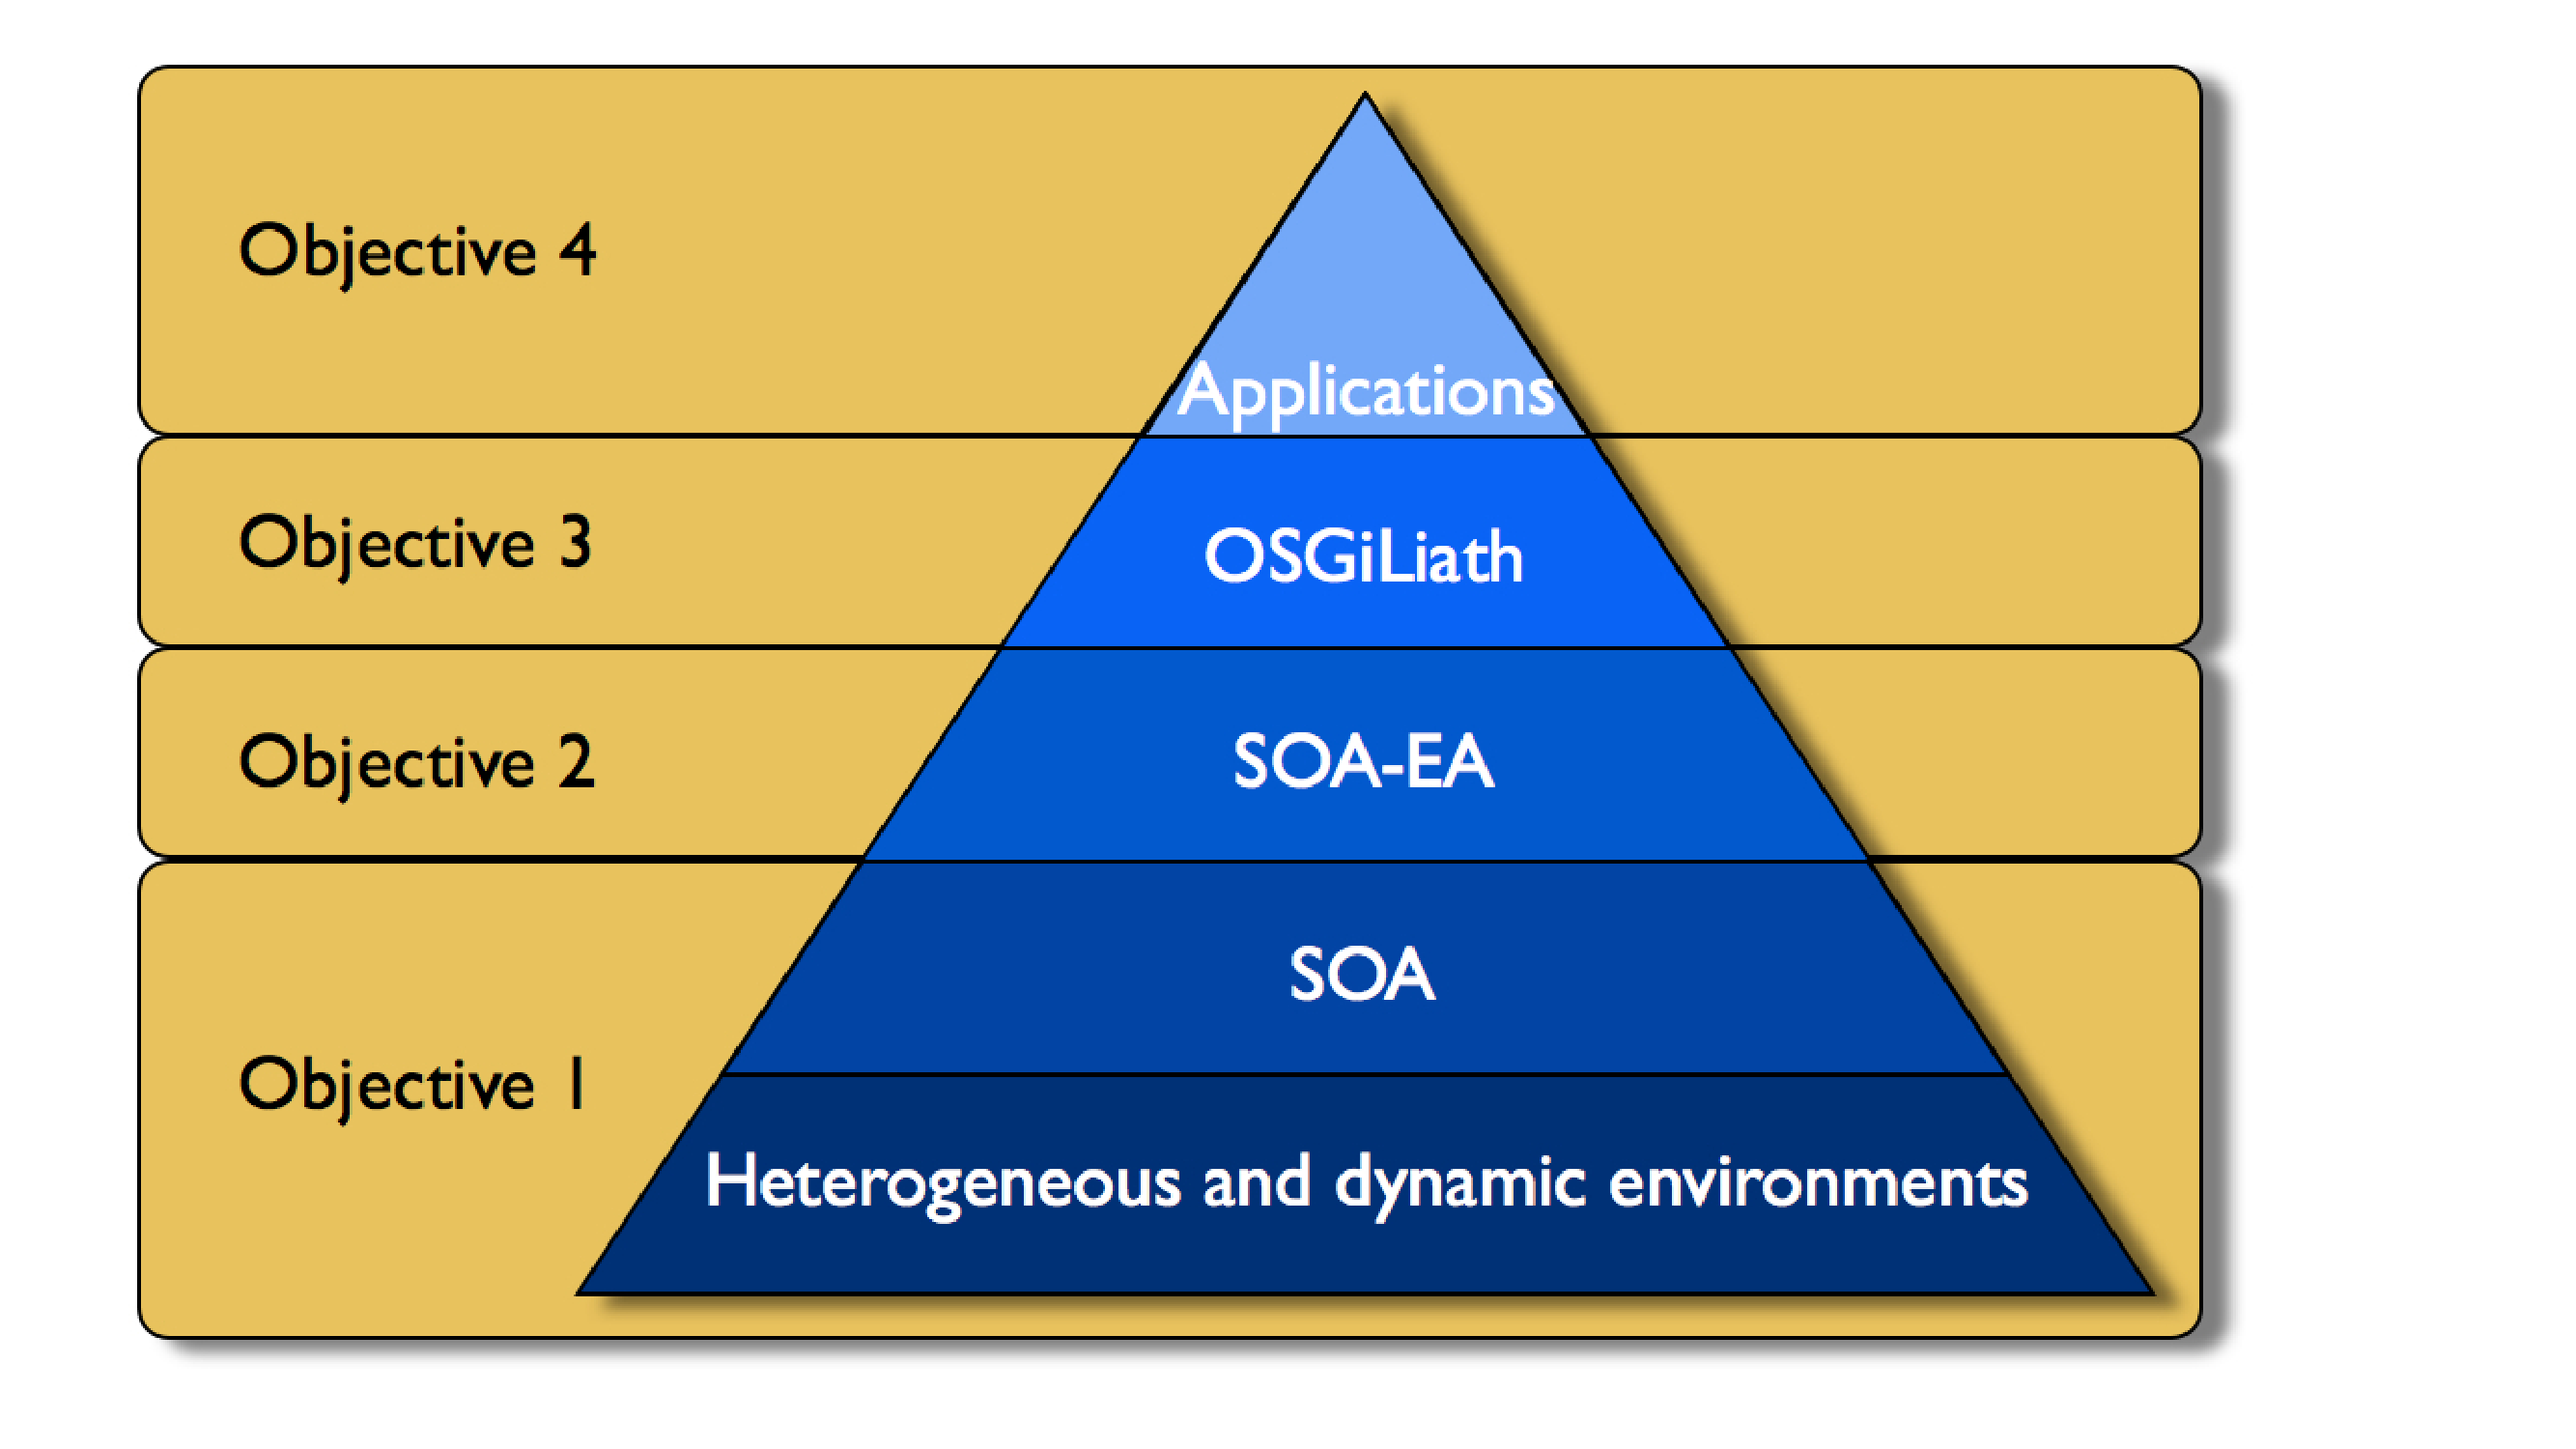
\includegraphics[scale =0.3] {gfx/intro/tesispiramide.pdf}
\caption{Summary of the objectives of this thesis.}
\label{fig:intro:piramid}
\end{SCfigure}

}{\myChapter{Introduction}\label{chap:introduction}}
\ifthenelse{\equal{\value{IncluyeCapitulo}}{2}}{\myChapter{Evolutionary Algorithms}\label{chap:distributedEAs} %Distributed o solo EAs? Si es distributed, �lo es! - JJ %FERGU: Tienes toda la raz�n

\begin{flushright}{\slshape
   I have called this principle, by which each slight variation,\\
   if useful,  is preserved, by the term of Natural Selection. } \\ \medskip
    --- {Charles Darwin, The Origin of Species (1859), Chapter III}
\end{flushright}

\minitoc\mtcskip
\vfill
%\lettrine{E}{volutionary} computation is a wide sub-field of  computational intelligence comprising several kinds of algorithms and its variants, techniques and tools \cite{eiben2003chapter1}. % en esta frase has aportado 0 bits de informaci�n. bla bla es un subcampo de bla bla que incluye bla bla - JJ


%The term \textsc{Evolutionary Algorithm} is used to describe a
%computer-based problem solving method that uses computational models
%whose design is inspired by the mechanisms of natural evolution \cite{darwin1859}. %aqu�
                                %la obligatoria cita de Darwin - JJ FERGU: Done

%In this algorithms a \textsc{population} of codified solutions (called \textsc{individuals})
%They are based on a % Di esto mejor: se crea una poblaci�n de
                       % soluciones codificadas...
%\textsc{population} of \textsc{individuals}, where the natural
%selection, caused by the environmental pressure, leads to an
%increase % bla bla miles de palabras que no has definido en este
         % contexto. En serio, puedes hacerlo mejor - JJ
%of the \textsc{fitness} of the individuals \cite{eiben2010whatis}. % no se incrementa el fitness de los individuos, sino de la poblaci�n. El de un individuo en particular puede disminuir. No incluyas afirmaciones discutibles, y m�s en campos donde el tribunal sea experto - JJ
%This fitness % define donde uses por primera vez. - JJ
%is an evaluation function that describes the quality of the solution
%of the problem being solved. % s� menos descriptivo y m�s formas. Una
                             % funci�n de qu� conjunto a qu� conjunto?
%Individuals within the population are combined and modified by means
%of \textsc{recombination} and \textsc{mutation} operators, creating
%new individuals to be added to the population. % o sea, �la poblaci�n
                                % aumenta? Imag�nate que no tienes ni
                                % idea de lo que es un algoritmos
                                % gen�tico - JJ


%FERGU: He comentado TODO lo de arriba por lo que viene aqu� a continuaci�n.


\lettrine{E}{volutionary} Algorithms are a set of bio-inspired techniques applied to optimization problems \cite{eiben2010whatis}, based on the process of natural selection \cite{darwin1859}. In this kind of algorithms, a \textsc{population} of codified solutions (called \textsc{individuals}) is created. The most adapted individuals have more chances to be selected for reproduction, so their offspring could inherit their genetic material. The level of adaptation of each solution is measured using a \textsc{fitness} function, that usually models the problem to solve.
%FERGU: Tambi�n he movido la figura del EA y pongo lo que viene a continuaci�n:

Initially the EAs were proposed as a fixed set of steps with different operators and data structures. Then, several ways to parallelize these algorithms were also presented, with new classifications and operations. Nowadays, new emerging trends that deal with new technologies (such as P2P or Cloud Computing) and new algorithmic methods (such as parameter adaptation) are being used. These trends require a new way to develop EAs taking into account some shortcomings, such as integration of heterogeneous elements or dynamic resources, and also to deal with fault-tolerance, churn, massive
scalability or decentralization.

As previously said in the introduction, the aim of this thesis is to facilitate the development, standardization, integration and dynamism in EAs. Therefore, in this chapter the classic classification of EAs is presented to clarify their common elements, together with the most extended models to parallelize these algorithms. This classification can be used as a base for the creation of new algorithms, establishing their similarities, to facilitate the {\em development}. Then, the new trends in EAs are also presented to summarize their benefits, but also their deficiencies and problems that should be addressed (such as {\em dynamism} of computing nodes or in the elements that form the EA). Finally, some of the most used frameworks to develop EAs are listed and analysed, to understand their capabilities and deficiencies (such as the lack of {\em standardization} and {\em integration}). This way, in following chapters, the design and development of interoperable, standardized and dynamic services for EAs will have a solid base to start.





%During the execution of the EAs, two different phases exist:
%\begin{description}
%\item[Exploration] Generation of new individuals to expand the search space. This is usually performed in the first iterations of the EA.
%\item[Explotation] Concentration in the neighbourhood of the best solutions.
%\end{description}
% No son fases. Suceden a la vez, solo que en diferentes
% proporciones. - JJ FERGU: Estaba comentado, no saldr� en la tesis.

%This chapter introduces a general overview of the most used types of Evolutionary Algorithms to clarify their common elements. Also, the most extended models to parallelize EAs are presented, to understand all their possible architectural possibilities. Finally, some of the most used frameworks to develop EAs are listed and analysed, to summarize their capabilities and lacks. This way, in following chapters, the design of services for EAs will have a solid base to start.



\section{Types of Evolutionary Algorithms}
\label{sec:distributed:types}
\lettrine{T}{he} general scheme of an EA, extracted from the work of \person{Eiben and Smith} \cite{eiben2010whatis} is described in Figure \ref{fig:basicscheme}. Although most of the EAs follow the scheme shown in this Figure, they have differences depending on the
representation of the solutions, the problems to solve, and other
features. A possible classification is presented in this chapter, 
taking into account the new approaches that cannot fit in the traditional 
taxonomy. This classification would help to clarify the elements that 
distinguish an algorithm from another (for example, the operators), 
and the existing similarities and differences, in order to establish  
a good starting point for designing services for EAs.

%hay un entorno algoritmo que hace
                                %esto mucho m�s chulo - JJ
                                %FERGU: s�, y lo uso en posteriores cap�tulos. Esto lo he copiado tal cual del libro de Eiben.
\begin{SaveVerbatim}{BasicEAtext} 
BEGIN
 INITIALISE population with random candidate solutions;
 EVALUATE each candidate;
 REPEAT UNTIL (TERMINATION CONDITION is satisfied) DO
   1 SELECT parents;
   2 RECOMBINE pairs of parents;
   3 MUTATE the resulting offspring;
   4 EVALUATE new candidates;
   3 SELECT individuals for the next generation;
 OD
END
\end{SaveVerbatim} 
%Parece COBOL. Qu� vintage - JJ FERGU: Ya xD �Lo cambio? Ya te digo, es como viene en el libro.

\begin{SCfigure}[][tb]
\begin{tabular}{|A|}
\hline
\footnotesize
\BUseVerbatim{BasicEAtext}
\\
\hline
\end{tabular}
\caption{General scheme of an evolutionary algorithm in pseudo-code}
\label{fig:basicscheme}
\end{SCfigure}


\subsection{Classic classification of EAs}
\label{subsec:classicEAs}
This subsection explains the traditional variants, according to
the book of \person{Eiben and Smith} \cite{eiben2003introduction}. These authors clarify that the features of an EA are:
\begin{itemize}
\item EAs are population based.
\item EAs mostly uses recombination to generate new individual from the existing ones.
\item EAs are stochastic.
\end{itemize} % �Esto aporta algo a lo que has dicho antes? �A tu
              % tesis? - JJ FERGU: explicado a continuaci�n
These are the elements that distinguish the EAs from another meta-heuristics (such as the Local Search \cite{aarts1997local}, for example).

% libro que tiene 10 a�os y que, hoy en d�a, no s� si es
% vigente. Adem�s, �es relevante para tu tesis? - JJ
% FERGU: La �ltima edici�n es de 2010 y se sigue vendiendo y citando.
% Es relevante para entender c�mo dise�ar los servicios, as� que 
% he a�adido un p�rrafo arriba, he dicho que es "most of the EAs" y a�ado las features, y digo que es la "classic"

\begin{description}
\item [Genetic Algorithms] These kind of algorithms were proposed by \person{Holland} \citep{holland1975adaptation}, and also studied by \person{Goldberg} \cite{goldberg1988genetic} and \person{Michalewicz} \cite{michalewicz1996genetic}. In this kind of EA, the representation of the solution is a string of numbers (usually binary), called \textsc{chromosome} (and sometimes \textsc{genome}). The individuals are selected proportionally to their fitness, and then \textsc{recombination} and/or \textsc{mutation} are applied to generate new individuals that will be introduced in the population. These algorithms have been used in different areas, such as function optimization \cite{michalewicz1996genetic}, combinatorial optimization \cite{Esparcia2009EVITA}, artificial intelligence in videogames \cite{Fernandez20111optimizing}, or generative art \cite{Garcia2013RGB}, among others. 

\item[Evolution Strategies] The Evolution Strategies (ES) are used to solve problems whose solution is included in the domain of real numbers. Their main difference with GAs is the inclusion of self-adaptation of the mutation rate, being coded in each individual \cite{eiben2005shared}. Also, the parent selection is performed randomly. ES have been applied in fields such as Evolutionary Robotics \cite{Garcia2012testing}.

\item[Evolutionary Programming] In Evolutionary Programming (EP), the representation of the solution depends on the nature of the problem being solved, for example, neural networks \cite{Castillo1999gprop} or Radial Basis Functions (RBFs) \cite{Gonzalez2003multiobjective} have been used as individuals.

\item[Genetic Programming] The objective of this technique is to
  create functions or programs to solve determined
  problems. Individual representation is frequently in the form of a tree,
  formed by operators (or {\em primitives}) and variables ({\em
    terminals}). These sets are usually fixed and known. The genome
  size is, therefore, variable, but the maximum size of the
  individuals is commonly fixed, to avoid high evaluation costs. GP has
  been used to evolve \definicion{LISP}{LISt Processing} programs
  \cite{Koza1990Tools}, or \definicion{XSLT}{eXtensible Stylesheet
    Language Transformations} scripts \cite{Garcia2008XSLT}, among
  others.

%Desde el trabajo de Michalewicz y, m�s todav�a, las EO, se trata
%simplemente de usar diferentes estructuras de datos y operadores. No
%merece la pena que hagas esa distinci�n y menos hoy en d�a (y menos
%en tu tesis) - JJ

\end{description}

\subsection{Other models} %FERGU: TODO cambiar este nombre?

Other EAs that do not match in the previous classification  have been proposed. For example \textsc{Differential Evolution}
(DE) \cite{storn1997differential}, \textsc{Estimation of Distribution
  Algorithms} (EDAs) \cite{larranaga2002estimation} or
\textsc{Bayesian Optimization Algorithms} \cite{pelikan2005bayesian}. 
%SEGURO QUE SON EAS? 
% Por supuesto que lo son y no encajan dentro de la r�gida
% clasificaci�n anterior. Por no mencionar EAs basados en pool u otro %FERGU: a�adido que no encajan (luego hablo del pool)
% tipo de algoritmos gen�ticos. Esto tienes que reescribirlo
% totalmente, suena a rancio, rancio... Adem�s, tienes algoritmos
% evolutivos celulares, coevolutivos, mem�ticos y miles de cosas m�s
% que no encajan en una definici�n. No es tu tesis, pero intenta
% sintetizar las tendencias en EAs para justificar la creaci�n de
% nuevos marcos de implementaci�n como los de tu tesis. - JJ FERGU: dijo que son other models, los otros EAs los presento a continuaci�n


%\subsection{Differential Evolution}
%Differential Evolution \cite{} also exploits a population of potential solutions. Three individuals are selected randomly from the population to create \textsc{random noisy vectors}. These vectors are recombined with original random individuals to create the \textsc{trial vectors}. These vectors are compared one by one with the original vector and the better of each comparison is kept for the next generation.

%Table \ref{tab:summaryEAs} shows the main differences between all this types of EAs. Note that we have selected the common features of each algorithm. For example, the replacement in GAs can be different from the generational one, or the representation can also be a real-value vector. 

%\begin{SCtable}[][t]
%\resizebox{11cm}{!}{
%\begin{tabular}{llllll}
%\hline
%				& Genetic algorithm 	 & Evolution Strategy  & Evolutionary Programming & Genetic Programming & Differential evolution  \\
%\hline\hline
%Representation  & Finite alphabet strings & Real-value vectors  & 					& Tree 				& Real-value vectors 	 \\
%Initialization  & \multicolumn{5}{c}{Multi-column} Random, depending of the problem and individual structure	 						 \\
%Selection 	& Fitness proportional 	& Random 				& 						& Fitness proportional & Random to create noisy vectors \\
%Recombination   & Genome crossover		& Genome crossover		& 						& Sub-tree exchange		& Random gene by gene			\\
%Mutation  		& Random 				& Gaussian perturbation	& 						& Random 				& Implicit in the noisy vectors	 \\
%Replacement		& Generational			& ($\mu,\lambda$) or ($\mu + \lambda$) &			& Generational 			& Compared with the original	 \\
%\hline
%\end{tabular}
%}
%\caption{Differences between the types of EAs.}
%\label{tab:summaryEAs}
%\end{SCtable}



Combining elements of all the previous algorithms with other heuristics is
the base of \textsc{Memetic Algorithms} (MAs). These algorithms are
based on the concept of {\em meme} % �por qu� small caps y no
                                % italica? - JJ %FERGU: Tengo tambi�n que homogeneizar el formato. Usar� SC para definir nuevos conceptos, he actualizado el issue.
proposed by \person{Dawkins}
\cite{dawkins2006selfish}. In this context, a meme is domain specific knowledge coded by a computational representation to the effective solving of a problem.

This kind of algorithms can be seen as an hybrid combination of the population-based evolution methods previously explained, coupled with some kind of local search. Initially, the hybridization was made just combining two o more methods with some kind of problem knowledge. For example combining a genetic algorithm with Simulated Annealing (SA) \cite{Rodriguez2012Hybrid}. The local search can be performed before, during, or after the evaluation. New trends, such as adaptive MAs \cite{ong2006classification} lead to the usage of several memes for searching and deciding dynamically which meme should be applied to each individual. For example, \person{Cowling \etal} �proposed the term \textsc{hyperheuristic} \cite{cowling2001hyperheuristic} as the strategy to choose the meme to be applied depending on the time and the region of the search space (or, in a brief, heuristic to choose memes).  Other examples are the work of \person{Krasnogor \etal} \cite{krasnogor2002multimeme}, where the 
inclusion of the memetic codification inside the individual chromosome
(\textsc{Multimemes}) to select which meme to use is applied;  or
codify a set of rules, as proposed by \person{Smith} \cite{smith2002co}
(\textsc{Co-evolving MAs}).

 % y esto es interesante para tu tesis
                            % porque... (no me vale porque tengo que
                            % rellenar el cap�tulo de estado del arte)
                            % - JJ FERGU: Esto lo explicaba en la secci�n conclusiones, pero lo pongo aqu� a continuaci�n.
In brief, the memetic algorithms can be seen as a composition of other algorithms. The integration should be as easy as possible to allow researchers develop new algorithms easily. Moreover, not only the way to combine the algorithms that conform the memetic one, but also how to dynamically select among these available memes. Thus, mechanisms to announce memes and automatically discovering and binding should be applied. %FERGU: TODO terminar esto y dejalo m�s claro a�n

\section{Parallel and Distributed Evolutionary Algorithms models}
\label{sec:distributed:parallel}
% �Inherentemente por qu�? �No querr�s decir trivialmente? Adem�s, no es tan trivial porque una vez que metes esquemas de inmigraci�n la cosa no es tan f�cil: quien emigra, cuando lo hace, como se incorpora en la poblaci�n... - JJ FERGU: A�adida cita a paper que lo dice
\lettrine{E}{volutionary} Algorithms are inherently parallelizable, since each individual can be considered as an independent unit \cite{Alba13parallel}. Thus, there exist several ways to parallelize: for example, fitness evaluation can be distributed into several slave machines, % lo que s�lo funciona si el trasiego es m�s r�pido que la evaluaci�n local, y s�lo para aquellos algoritmos en los que la evaluaci�n de un individuo s�lo dependa del mismo: hay esquemas de escalado del fitness o algoritmos coevolutivos en los que esto no tiene por qu� funcionar - JJ FERGU: Digo entonces que son ejemplos
or the population can be distributed among different nodes to be
evolved at the same time. In 2002, two main types of parallelization
models for EAs were classified by \person{Alba and Tomassini} in
\cite{alba2002parallelism}: \textsc{Global parallel EAs} and
\textsc{Spatially structured EAs}. However, with the aim of new
technologies and architectures, such as P2P, new ways to parallelize
EAs have been proposed. In this section, the differences of the existing classification
with these new trends are explained, and the requirements of each one are presented.

% �Y a qui�n le importa lo que pas� en 2002?
                        % Haz un esfuerzo y haz t� una clasificaci�n
                        % en 2014 - JJ FERGU: Digo que hay nuevas formas

\subsection{Traditional parallelization classification}

As this classification was established in 2002, issues such as fault-tolerance, churn, massive
scalability or decentralization were not taken into consideration.  % di
                                % desde el principio que esto es lo
                                % que vas a hacer - JJ FERGU: puesto en la intro del cap�tulo
The number of computational nodes are fixed during the whole execution and both the network and the nodes are reliable and trustworthy.

\subsubsection{Global parallel evolutionary algorithms} % No s� si
                                % deber�a ser una subsecci�n o
                                % simplemente un p�rrafo - JJ FERGUSON: es una sub-subsecci�n, no se ve el n�mero de subsecci�n, no sale en los �ndices, y al compilar se ve bonito
In this model, also called \textsc{Farming model}, \textsc{Master-Slave} or \textsc{Centralized EA}, the parallelism is applied at evaluation level, where a central node coordinate several slave nodes. The central node executes the EA in a sequential way, but distributes the individuals of the population to the slaves just for being evaluated. Figure \ref{fig:masterslave} depicts this situation.

\begin{SCfigure}[20][tb]
\centering
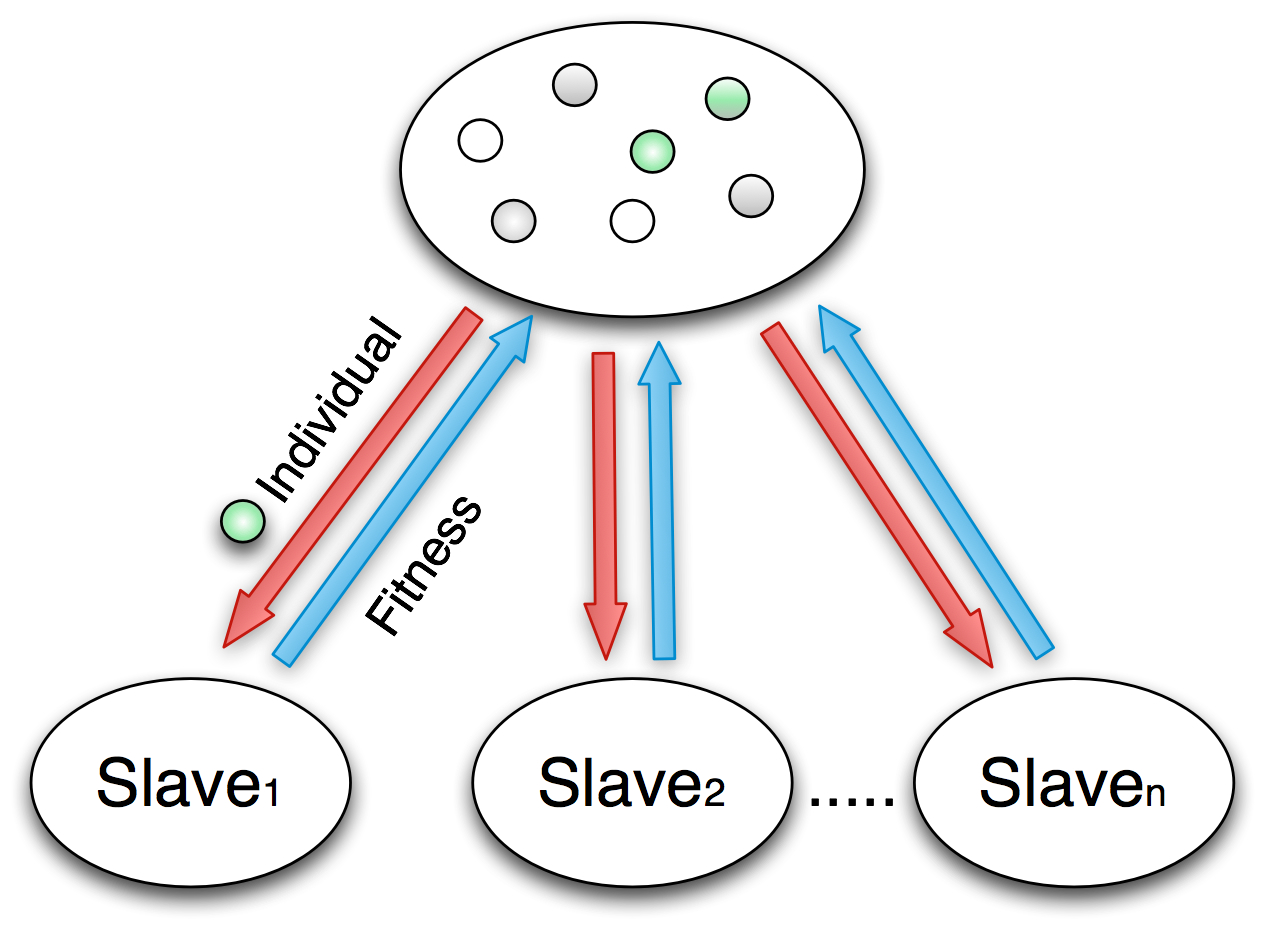
\includegraphics[width=20pc]{gfx/distributed/masterslave.jpg}
\caption{Master-slave model.}
\label{fig:masterslave}
\end{SCfigure}

\subsubsection{Spatially structured algorithms}
The parallelism is performed at population level, that is, dividing the population among the different computing elements. Depending on how the distribution is performed we have:
\begin{description}
\item[Coarse-grained approach] One of the most usual approaches is the \textsc{Island model}, where a number of nodes executes simultaneously the EA, working with different sub-populations at the same time. Each certain number of generations some individuals are interchanged (migrated) between populations. Figure \ref{fig:ring} shows this model with a ring topology.

\begin{SCfigure}[20][tb]
\centering
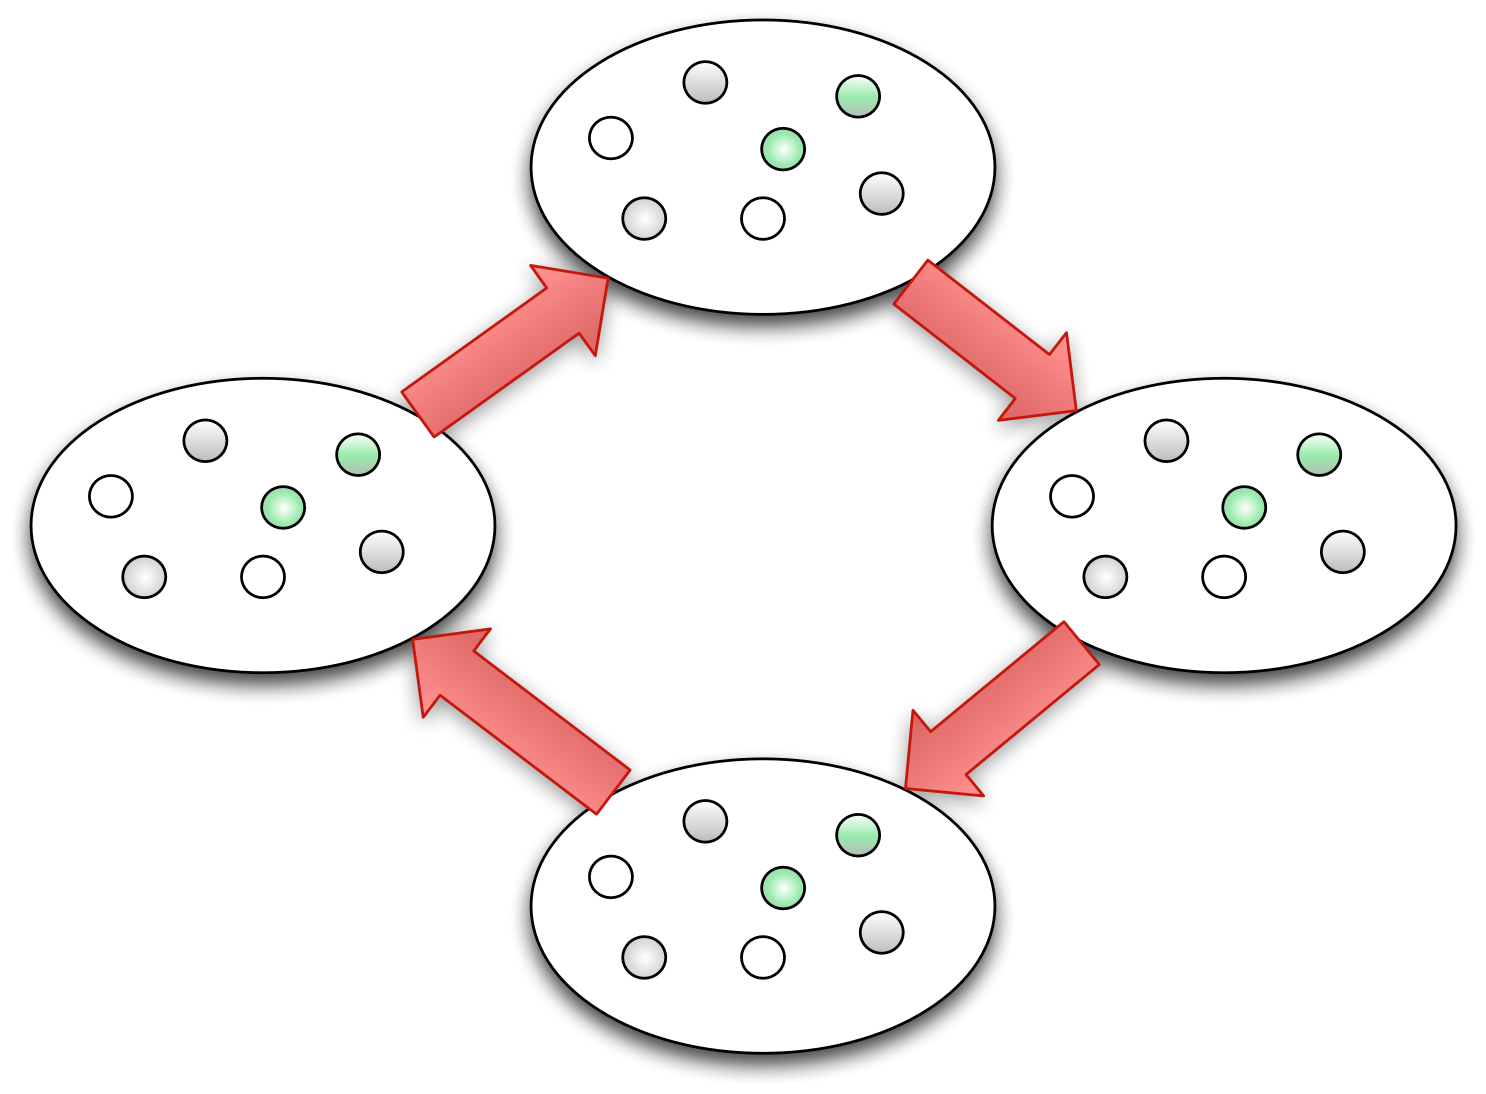
\includegraphics[width=20pc]{gfx/distributed/ring.jpg}
\caption{Island model scheme using a neighbourhood ring topology.}
\label{fig:ring}
\end{SCfigure}

\item[Fine-grained approach] In this approach, also called \textsc{Cellular EA} (CEA), each node has one individual of the population, and selection and reproduction are limited to the individuals of the neighbourhood of the node \cite{CELLULAR}. Usually a bi-dimensional grid is used as topology, such as the one showed in the Figure \ref{fig:cellular}.

\begin{SCfigure}[20][tb]
\centering
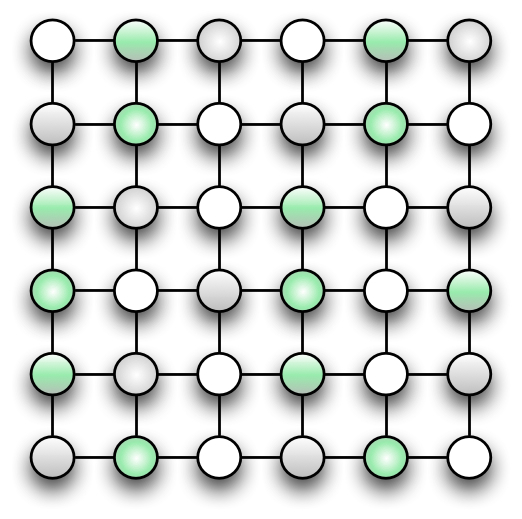
\includegraphics[width=5cm]{gfx/distributed/cellular.jpg}
\caption{Cellular Evolutionary Algorithm.}
\label{fig:cellular}
\end{SCfigure}

\end{description}

\subsection{New trends on parallel EAs} 
\label{chap:distributed:newtrendson}
% �Por qu� no convencionales?
                                % - JJ FERGU: Cambiado a new trends

When developing distributed and parallel EAs (or any distributed system in general), 
we should deal with the {\em Fallacies of Distributed Computing}, proposed by \person{Peter Deutsch}
and then explained by \person{Rotem-Gal-Oz} in \cite{rotem2006fallacies}.

\begin{enumerate}
\item The network is reliable.
\item Latency is zero.
\item Bandwidth is infinite.
\item The network is secure. 
\item Topology doesn't change. 
\item There is one administrator. 
\item Transport cost is zero. 
\item The network is homogeneous.
\end{enumerate}

These fallacies were not taken into account in the previous classification. %why? - JJ
 However, with the advent of new
technologies, such as cloud computing,
\definicion{P2P}{Peer-to-peer} networks, or the usage of heterogeneous
hardware, new approaches have been proposed. % that take into account, for instance, unreliability... jolines, explica las cosas bien - JJ 
 Distributed EAs can be
executed in other computing elements different than the classic
computers. For example, in mobile devices \cite{Garcia2009Mobile},
``smart dust'' \cite{Rollings2008smartdust} or inside robots, 
learning from the environment in an on-line manner \cite{Garcia2012testing}. But with
the advancement of the Internet, where millions of nodes can
co-operate, and whose behaviour is not totally controlled or
predicted, is when new distributed approaches have become more
evident.  

% �Esto es una clasificaci�n? �A qu� nivel est�s clasificando? �C�mo
% encaja esto dentro de lo que has escrito en los primeros p�rrafos?
% �Y de TU TESIS? - JJ FERGU: quitada la clasificaci�n
%\subsubsection{P2P evolutionary algorithms}

P2P systems are parallel infrastructures composed by a large number of
resources, % eso no define los sistemas P2P, sino sus
           % conexiones. Pueden tener 3 recursos. Adem�s, �qu� diablos
           % significa recurso en este contexto? - JJ
without any central server \cite{steinmetz2005peer}. In practice, the
resources in these networks can appear or disappear dynamically. These
platforms can be used to execute large instances of problems, taking
advantage of the massive scalability that these systems potentially
offer. %La escalabilidad no la da el sistema, sino el algoritmo. Algo
       %tan f�cil como una b�squeda puede colapsar la red si el
       %algoritmo no es el correcto. Mira esto: Loo, Boon Thau, et al. "Measurement and Analysis of Ultrapeer-based P2P Search Networks." (2003).
 An example of one EA that has been designed to take advantage of these systems, is
  \definicion{EvAg}{Evolvable Agent}, proposed by \person{Laredo \etal}�\cite{laredo2010evag}. This algorithm
  uses a decentralized population, where each peer has a single
 individual, and new individuals are created combining the ones in
 their current neighbours. % hala, non-sequitur. �Un ejemplo? �El m�s
                           % guay? �El m�s actual? �Soluciona qu�
                           % problemas y como? - JJ FERGU: un ejemplo, y el problema que resuelve, a�adido
To solve the problem of the dynamic topology, the population structure is maintained using the \textsc{newcast}
protocol \cite{jelasity2003newscast}: each node has a cache of
neighbours that can be interchanged and combined. Figure
\ref{fig:evag} shows this algorithm and its population
structure. Results show that this algorithm outperforms tuned GAs,
using less links that a panmictic (i.e. fully connected) population. 
% resolviendo el problema de conectividad fija (con DHT) o la introducci�n de nodos destacados (ultrapeers). Esto es un protocolo tipo gossip que podr�as mencionar y en todo caso el primer sistema P2P de EAs no fue este, sino DREAM, de donde desciende - JJ

\begin{SCfigure}[20][tb]
\centering
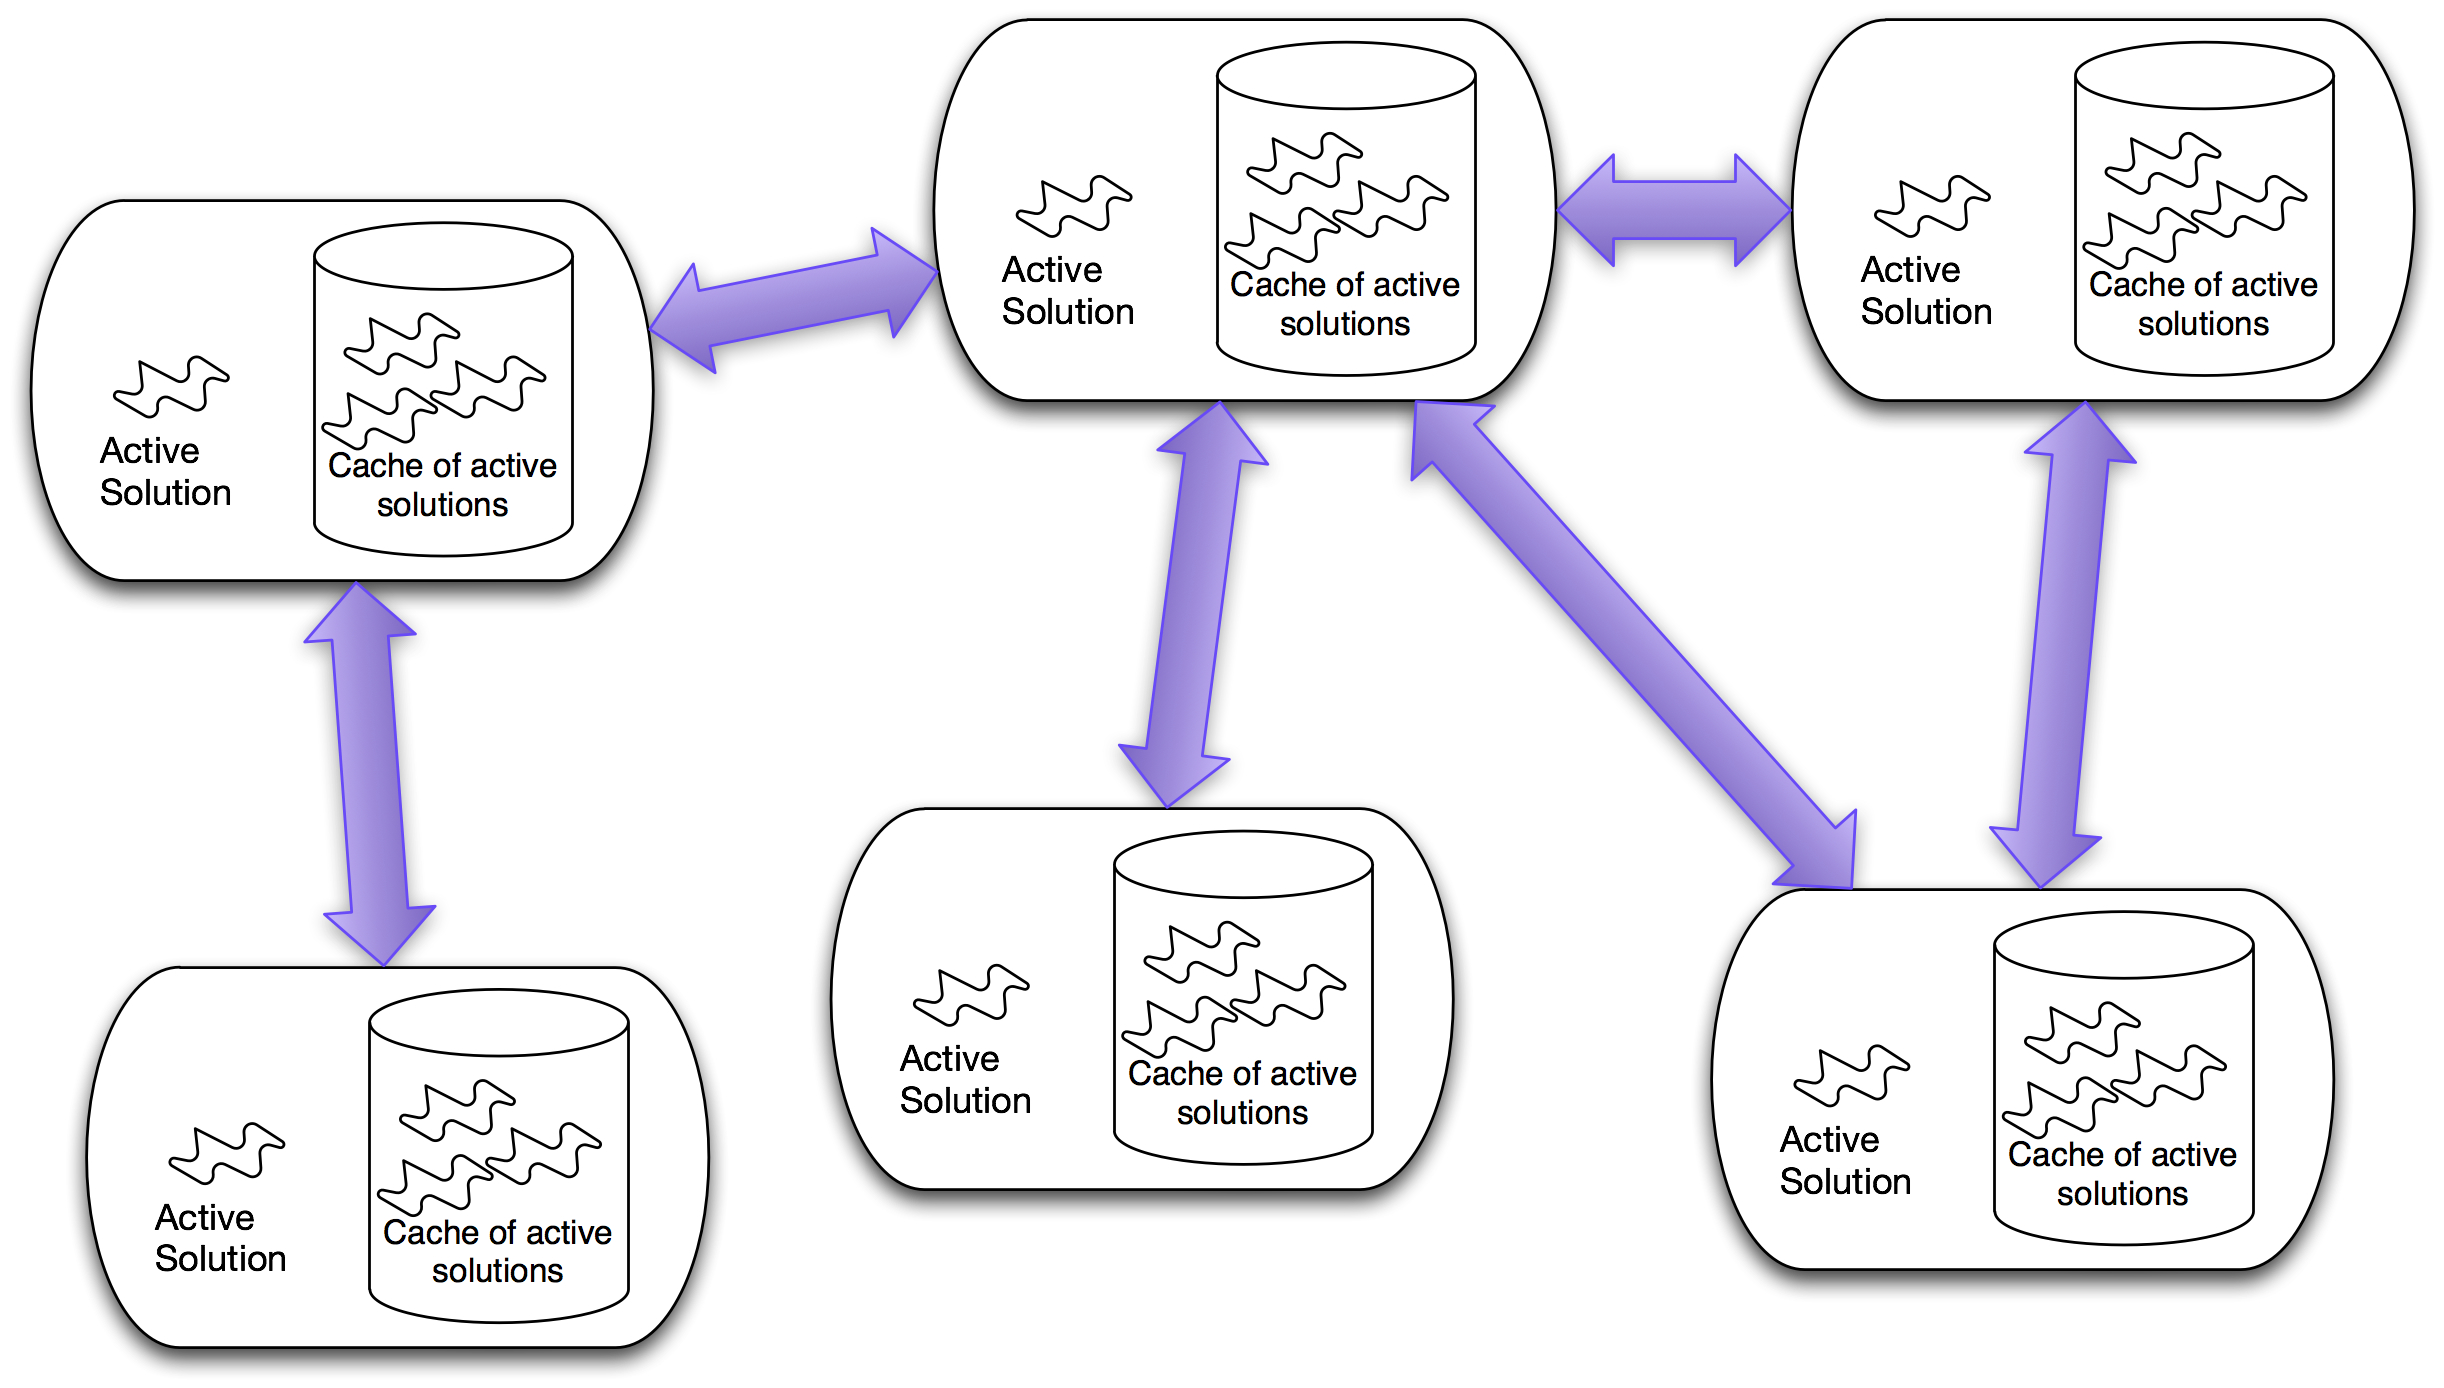
\includegraphics[width=26pc]{gfx/distributed/evag.jpg}
\caption{P2P Evolutionary Algorithm: EvAg.}
\label{fig:evag}
\end{SCfigure}

%\subsubsection{Pool-based algorithms}
Technologies such as non-relational databases % �cu�les? �Por d�nde? �C�mo? FERGU: est�n explicadas despu�s
lead to \textsc{Pool-based EAs} \cite{merelo2010fluid}, where the computational nodes
exchange individuals using a shared pool. 
Although this can be seen as a farming model, there are differences 
in how the data flow of individuals is managed.
% si son individuos para
                                % evaluar, se trata simplemente de
                                % "farming". Lo interesante es el
                                % flujo de datos de estos
                                % individuos. �Y cita nuestros papers
                                % y otros, como el de Gagn�! - JJ FERGU: A�adida tu cita (aunque m�s tarde cito todos)
This allows massive scalability with a heterogeneous underlying
structure. This pool can be used as the global population, and the
nodes asynchronously read and evaluate the individuals. It can also be used
to share individuals among islands. % una posibilidad... y otra
                      % posibilidad... clasificaci�n de tipo
                      % Borges. �Hay que ser exhaustivo y describir de
                      % qu� se trata este tipo de algoritmo! - JJ FERGU: reescrito
This can lead to automatic load-balancing and synchronization,
allowing the addition and removal of nodes. % s�
                                % consistente. "computer" "node"
                                % "individual". �No ibas a establecer
                                % la terminolog�a en este cap�tulo? - JJ FERGU: voy a usar "nodo" como elemento de c�mputo
Different technologies can be used. For example, in the work of
\person{Meri \etal},  the pool used is based on the
Dropbox\texttrademark\, or SugarSync\texttrademark\ file storage
services. Other authors propose the use of non-relational databases,
such as the work of \person{Merelo \etal} \cite{merelo2010fluid},
using FluidDB\texttrademark. In \cite{merelo2012pool} the same authors
improve the design, proposing an asynchronous, fault-tolerant, and
scalable dEA, based on the object store CouchDB\texttrademark. The
results show that adding clients could not scale, but increase the
fault tolerance. Also, their experimentation shows a good methodology
for designing EAs in heterogeneous distributed systems, which have the
impossibility of analytic performance prediction. 

%\subsubsection{Grid and volunteer computing} %Clasificaci�n tipo
                                %Borges. la computaci�n voluntaria
                                %puede ser "cl�sica", "basada en pool"
                                %o incluso P2P (dependiendo del
                                %cliente). FERGU: quitada clasificaci�n
Other systems, such as Grids \cite{grid1} are distributed computing systems that allow sharing
geographically distributed resources to solve large scale
problems. % grid es el predecesor de la computaci�n nube. Tampoco
          % tiene mucho que ver con la computaci�n voluntaria, salvo
          % que se le llama "desktop grid". Sep�ralos (y justifica
          % bien la clasicaci�n real). - JJ
Several works that describe EAs being executed
% no uses "There exist" como en el chiste de Gila "Hay alguien que ha
% hecho algo malo..." - JJ FERGU: Cambiado 
in these systems have been presented \citep{grid8,grid4,grid10}. \textsc{Volunteer
  computing} \cite{anderson2005high} proposes the creation of
infrastructures to allow people donate CPU cycles for a combined
computational effort. Its main difference with grid computing is the
presence of un-trusted resources: for example, some nodes could return
intentionally wrong results, so it requires the possibility of
replication of the results to be validated. % �posibilidad de replicaci�n? - JJ FERGU: arreglado
Also, the control of the participating nodes is not
maintained by the experiment launcher. EAs have been executed in these
systems, using several techniques, such as virtualization
\cite{Fernandez2013BOINC} or ``parasite'' computing
\cite{Merelo2007browser}. % Esta no es par�sita, los participantes
                          % estaban avisados - JJ

Summarizing, with these new trends in parallel EAs, researchers must deal 
with heterogeneous hardware and different communication protocols, but also
 with dynamic, non-centralized or uncontrolled environments. %FERGU: ...enlazando con la tesis...

 


\section{Parameter adaptation in Evolutionary Algorithms}
\label{chap:distributed:parameteradapt}
% y esto viene a cuento porque... - JJ

\lettrine{O}{ne} of the greater challenges of the EC field is to find
the appropriate values for EAs parameters
\cite{Eiben12Parameters}. Usually, these parameters are established by
convention or after several test runs, for example. However,
practitioners need to put effort on finding these values in order to
attain significant performance in their EAs, even taking into account
other variables, such as the computational power of the machines
used.

\subsection{Parameter Control and Parameter Tuning}
\label{chap:distributed:pcontroltuning}
There are two different approaches for algorithm parameter setting  in EC: {\em parameter control} and {\em parameter tuning} \cite{ParameterControlEiben99}. The first one refers to setting up a number of parameters for the Evolutionary Algorithm (EA) and changing them in running time. The parameter tuning consists in establishing a good set of parameters {\em before} the run (and not changing these parameters during runtime).

\person{Eiben}, in \cite{ParameterControlEiben07} proposes the next taxonomy for the parameter control, according to {\em how} the are changes made:
\begin{itemize}
\item Deterministic methods: changes to a parameter are triggered by a deterministic rule (for example, increase mutation rate after certain number of generations).
\item Adaptive methods: parameters change depending on some behaviour (for example, increase mutation rate if the average fitness of the population stagnates).
\item Self-adaptive methods: parameters are encoded within the chromosome of the individuals of the population (for example, mutation rate can be a value in the chromosome).
\end{itemize}

Other classifications for control techniques in EAs are presented in that work. For example, regarding to {\em what} is changed:
\begin{itemize}
\item Representation
\item Evaluation function
\item Variation of operators and their rates
\item Selection operators
\item Replacement operator
\item Population
\end{itemize}

Finally, a third classification can be obtained according to what evidence is available:
\begin{itemize}
\item Absolute evidence: The parameter changes if a rule is activated when an specific event occurs. For example: increase mutation rate when diversity drops. In this case, human knowledge is necessary to model these rules.
\item Relative evidence: Parameters are compared with the fitness of their produced offspring and the best values are rewarded. It is not deterministic.
\end{itemize}

These classifications can be used to establish a way to manage or update the parameters 
in the development of algorithms. For example, it should be necessary to allow a direct
 access to each parameter and sources of information of the EA, independently of the actual 
 state of the algorithm. A possible solution to manage 
the dynamic parameters, and the information of the elements that conform the EA, is proposed in next chapters.
% Vale, llego aqu� y todav�a no s� qu� diablos tiene que ver con los
% SOA y el OSGi y OSGILIATH - JJ FERGU: estoy cambiando este cap�tulo para indicar los problemas en desarrollo, integraci�n, estandarizaci�n y dinamismo en EAs. Luego dir� "necesitamos una soluci�n para esto!" (y a�adido el p�rrafo de arriba)

\subsection{Adaptation in heterogeneous hardware}
\label{subsec:distributed:adapthetero}
Adapting algorithm parameters to available computational resources
leads to improved performance (see the work of \person{Hamadi and
  Schoenauer} \cite{AutomaticallyConfiguringStyles12}). An easy way to
take advantage of the available resources is  balancing the workload
\cite{Garamendi2006Parallel} to distribute it across multiple
nodes. % �elements, computers, individuals, nodes? - JJ fERGU: cambiado a nodos
However, assigning the same tasks to each node on heterogeneous
clusters may result in suboptimal performance (as shown by
\person{Bohn and Lamont} \cite{LoadBalancingBohn02}). Parameters of an
algorithm could also be adapted to increase the performance of the
whole system. For example, the population size in EAs is the key to
obtain good performance, because it has % �Gram�tica! - JJ FERGU: qu� error hay? (lo has corregido, no?)
 effect on the quality of the solution and the time spent during the run \cite{ShrinkageLaredo09}. This parameter has been studied as a fixed \cite{SizingHarik99} or adaptive parameter during runtime \cite{AdaptiveLobo07,SelfRegulatedSizeFernandes06}, but without taking into account the computational power of each machine in a heterogeneous cluster. 

The adaptation of an algorithm can be useful to leverage different hardware environments.
One of the problems in parameter adaptation in heterogeneous clusters is 
the representation of the computational load. It depends on the algorithm, size of the problem, programming 
language, compiler or hardware characteristics, and the results obtained from artificial 
benchmarks (such as  Linpack \cite{LinpackEndo10}) should not be extolled as identificative 
of the system performance \cite{LinpackDongarra03}. For example, in the work of \person{Garamendi 
\etal} \cite{Garamendi2006Parallel},  a small benchmark was executed in all nodes at the beginning
of the algorithm in order to distribute individuals of an Evolutionary
Strategy, following a master-slave model. % but... - JJ FERGU: es lo siguiente (lo enlazo con However)
However, the computational load by artificial benchmarks may not accurately 
 represent the correct load of the algorithm, so, information 
 about the algorithm itself should be used for calibration. % sez who? FERGU: TODO buscar la referencia que encontr�!
                                % �Esto es tu tesis? - JJ FERGU: esto es para la parte de homoheterosize, lo pongo aqu� o all�?

In other works, there is no direct relation between the algorithm parameters and 
computational resources of the nodes. % sez who again? - JJ
For example, \person{Dom\'inguez \etal} \cite{Dominguez13HydroCM} 
divided the available devices into ``faster'' and ``slower'' nodes to create a distributed hybrid 
meta-heuristic that combines two different EAs: Genetic Algorithms and Simulated
Annealing. Their system executes the heavy (in computational
terms) algorithms (GAs) in the faster nodes (computational devices), and
simpler meta-heuristics (SA) in the slower ones, obtaining better results
than other configurations.  \person{Gong \etal} in \cite{Gong2005HeterogeneousTopology} also ordered 
the nodes by their computational power to test different topology configurations in a distributed EA.
Besides,  ordering the nodes taking into account 
only their previously known computational resources, the results of the previous works were not compared with executions on a homogeneous 
cluster to validate if the adaptation takes advantage of the heterogeneity 
of the cluster.

The heterogeneous computational performance of nodes or network speed can affect the performance of an algorithm. In \cite{Alba2002Heterogeneous},
 \person{Alba \etal} compared a distributed Genetic Algorithm (dGA), one of
 the sub-types of EAs, on homogeneous and heterogeneous clusters. 
 Super-linear performance in terms of iterations was obtained in the heterogeneous ones,
 being more efficient than the same algorithm running on homogeneous
 machines. However, the parameter setting was the same in both
 clusters and they did not adapt the parameters to the machines used.

 Adapting algorithm parameters to different nodes % ahora
                                % computational nodes - JJ FERGU: todo va a ser nodes ahora (cambiado a different)
derives in heterogeneous parameter sets. These sets can improve the results in homogeneous hardware, for example, setting a random set of parameters in each homogeneous node can also increase the
performance of a distributed Genetic Algorithm, as explained by \person{Gong
and Fukunaga} in \cite{Gong2011HeterogeneousParameters}. That model
outperformed a tuned canonical dGA with the same parameter values in
all islands. Also, adapting the migration rate produced better
results than homogeneous periods, as explained by \person{Salto and Alba} in
\cite{Salto2012HeterogeneousMigration}. This indicates that heterogeneous parameters
 may lead to an increase of performance, so it is necessary to validate if the 
 performance is due to the parameter set or to the heterogeneous
 devices combination. The way to access  the elements that conform 
 an EA (including their parameters) proposed in this thesis will be used 
 in next chapters to address this issue.


 % que es lo que vamos a hacer en esta tesis. O
                      % as�. - JJ FERGU: puesto �est� bien?


\section{Development of Evolutionary Algorithms} %FERGU: Cambiado t�tulo de la secci�n
\lettrine{O}{ne} of the aims of this thesis is to facilitate the standardization, 
integration and development of EAs.
% Y esto viene a cuento porque... la "narrativa" de este cap�tulo
% tienes que hacerla al principio del mismo, integrarlo todo en TU
% TESIS a la vez que estableces el estado del arte - JJ FERGU: a�adido arriba

 % cada vez que dices There exist, $deity mata a un gatito - JJ FERGU: Okis, los quito todos
This is due to the existing large number of frameworks for Evolutionary
Algorithms. 
Practically every programming language has its own implementation of the basic elements
that form an EA. This implies a large effort made in each one, giving
that these elements are not compatible among them. It is also
difficult to migrate the code from a framework to another, mainly due
to design choices, such as the existence of hidden global variables or
language specific features (such as functional programming
\cite{Cruz2013Erlang}). This is important for example, to integrate and reuse 
the elements of the frameworks in other systems (such as enterprise servers, for example). 
However, is in the field of Open Science \cite{Altunay2011OpenScience} where the integration and standardization of
the elements that conform an EA can take advantage, facilitating the re-use and access 
to existing software, systems, data, and results.
%FERGU: DONE
 % Y migrar c�digo es importante porque... - JJ

% di lo que es importante: genericidad, comunicaci�n,
% prestaciones... Y eval�a cada framework con respecto a esto para
% finalmente decir que tu framework va a ser mejor, pero recuerda que
% tu tesis no es tu framework - JJ

In this section, the genericity, communication and features of the 
development of EAs and existing frameworks are explained and compared 
to evaluate their benefits and shortcomings. 

\subsection{Design of EAs}
\label{sec:distributed:design}
The work of \person{Gagn\'e and Parizeau} \cite{GENERICITY05} established six criteria to qualify the genericity of a framework for EAs. 

\begin{itemize}
% resalta algo, hombre - JJ FERGU: hecho
\item {\em Generic representation}: independence of the structure of the individuals. 

\item {\em Generic fitness}: Individual fitness should be as independent as possible from the selection operators and individual representation. That means that the fitness evaluation should be outside of the implementation of the individuals (for example, not implementing the fitness in the class that implements the individual). 

\item {\em Generic operations}: operations should be used in conjunction with others and have minimal side effects. For example, a multi-parent reproduction (crossover with more than two parents, as presented by \person{Eiben et al.} \cite{EibenMultiparent97}) requires separation of the concept crossover with only two elements, so the abstract concept of crossover  should accept a list of individuals. Also, new operations can be created without affect the existing ones, allowing the interaction of a non-limited number of operators. Finally, the granularity of the design of the operators should be equilibrated, not being neither too coarse (may limit the flexibility to create new operators) nor too fine (could be difficult to integrate all the operators).

\item {\em Generic evolutionary model}: As explained in Section \ref{subsec:classicEAs}, % �d�nde? - JJ FERGU: hecho
there exist different ways to model an EA leading to different algorithms (for example, a steady-state GA versus a generational GA, or a GA versus ES). Operators should be independent of the evolutionary model, being possible the change from a model to another. 

\item {\em Parameter management}: parameters, such as the population size, may be modified during runtime. Also, a good framework should accept the addition of new parameters.

\item {\em Configurable output}: the output should be configurable. This is due to different statistics that could be used depending on the EA: for example, the tree depth in GP. Also, different outputs (console, files) should be managed.

\end{itemize}

 These issues should be accomplished to develop new algorithms or operators, with independence of the programming language used. However, as will be explained in next chapters, new models of design and development can extend the previous criteria.

\subsection{Frameworks for EAs}
\label{subsec:soaea:fworks}
Over the large number of available frameworks (see \cite{SURVEYMOFS} for a complete survey) a representation of them has been selected to explain their shortcomings, that will be addressed in this thesis.

 % se est� quedando sin gatitos - JJ FERGU: Quitado el There exist
Object Oriented programming is used in several frameworks, such as Al\-go\-rithm::Evo\-lu\-tionary \cite{PERL}, \definicion{METCO}{Metaheuristic-based Extensible Tool for Collaborative Optimization} \cite{Leon2009metco},
\definicion{JCLEC}{Java Class Library for Evolutionary Computation} \cite{JCLEC} or jMetal \cite{JMETAL}. 
 Users implement specific interfaces of these frameworks ({\em
   individual} or {\em crossover}, for example) and they group them in the source
 code. For example, creating an operator object that groups several
 operators. However, these frameworks are not compatible among them.
 For example, the operators created in JCLEC can not be used directly in jMetal
 (despite both are programmed in Java). %Also, they can not control the
 %services (operators) outside the source code.

%\subsection{Parallel frameworks} % y Borges sin
                                % animales. Algorithm::Evolutionary
                                % puede ser paralelo los paralelos
                                % orientados a objetos - JJ FERGU: quitadas todas las subsecciones
Parallelism and distribution are possible in other frameworks, such as
MALLBA \citep{MALLBA}, \definicion{DREAM}{Distributed Resource
  Evolutionary Algorithm Machine} \citep{DREAM} or
\definicion{ECJ}{Evolutionary Computation in Java} \citep{ECJ}, but 
using external libraries (such as \definicion{MPI}{Message Passing Interface} or \definicion{DRM}{Distributed Resource Machine}), so the code that uses these
libraries is mixed with the algorithm's code.


 Even being distributed, these frameworks can not communicate with
 each other. This implies an extra effort to combine the capabilities 
 that a framework can offer to other frameworks or other programs (for example, a web server). %lo que es un problema por... - JJ FERGU: puesto
  HeuristicLab \citep{HEURISTICLAB} is one of the few plug-in and service oriented frameworks. It uses web services for communication, but only to distribute the load, after consulting a central database of available jobs. Finally, %the only service oriented optimization framework is
 gridUFO is a service oriented framework \citep{gridUFO}, but it only allows the modification of the objective function and the addition of whole algorithms, without combining existing services.  Table \ref{tab:frameworks} shows a summary of the previous frameworks.


\begin{SCtable}[][t]
\resizebox{11cm}{!}{
\begin{tabular}{llllll}
\hline
\rowcolor{colorCorporativoSuave}Name		&  Design 	 & Language 	& Distribution 	& License  		& Last version	\\
\hline\hline
\rowcolor{colorCorporativoMasSuave}ECJ		& OO		& Java		& Sockets   	& Academic Free Lic. 	& 2013		\\
\rowcolor{colorCorporativoSuave}MALLBA		& OO		& C++		& MPI		& Freeware		& 2010	\\
\rowcolor{colorCorporativoMasSuave}jMetal		& OO		& Java		& N/A		& GNU/LGPL 		&2013		\\
\rowcolor{colorCorporativoSuave}DREAM		& OO		& Java		& DRM		& GNU/GPL   		& 2003		\\
\rowcolor{colorCorporativoMasSuave}ParadiseEO	& OO		& C++		& MPI		& CeCILL	   	& 2012		\\
\rowcolor{colorCorporativoSuave}HeuristicLab	& OO/PO 	& .NET		& Web-Services	& GNU/GPL		& 2013			\\
\rowcolor{colorCorporativoMasSuave}METCO		& OO		& C++		& MPI		& N/A	   		& 2009	\\
\rowcolor{colorCorporativoSuave}JCLEC		& OO		& Java		& N/A		& GNU/GL   		&	2013 \\
\rowcolor{colorCorporativoMasSuave}Algorithm::Evol.& OO		& Perl		& N/A		& GNU/GPL  		& 2013	\\
\rowcolor{colorCorporativoSuave}gridUFO		&SO		& Java		& Web Services	& N/A  			& 	2010 \\
\hline
%OSGiLiath	&OO/SO/PO 	& 2010			& Java		& Distributed OSGi	& GNU/GPL  	& Lifecycle management	\\
\end{tabular}
}
\caption{Comparison of EA frameworks. OO=Object-Oriented, SO=Service Oriented, PO=Plug-in Oriented}
\label{tab:frameworks}
\end{SCtable}
% qu� pasa con DEAP? - JJ http://code.google.com/p/deap/ �Seguro que
% no hay m�s? FERGU: s�, hay m�s (a�ado un survey) pero digo al principio que hemos hecho una selecci�n

In brief, although these frameworks follow the six criteria for genericity 
proposed by \person{Gagn{\'e} and Parizeau} previously explained, they present some shortcomings when it is needed to develop
or add new features: the user is forced to modify the source code
or stop the execution to add new functionalities (like load balancing,
dynamic control of operators, or an user interface).


%\subsection{Volunteer computing frameworks} FERGU: enlazado con lo anterior
Other frameworks, not focused on EAs, can be used to deal with some of the issues, such as dynamism in nodes. \definicion{BOINC}{Berkeley Open Infrastructure for Network Computing} is one of the most used frameworks in volunteer computing. This middleware follows a master-slave architecture, where the server is in charge of hosting the project experiments and the creation and distribution of jobs \cite{Fernandez2013BOINC}. Clients ask the server for works, download information, compute data and upload the results. EAs have been used in BOINC, such as the work of \person{Fern\'andez \etal} \cite{Fernandez2013BOINC}. Other authors imitate this architecture using a browser-based scheme \cite{Merelo2007browser} to distribute fitness evaluations among clients without installing any other software. Previous systems have the possibility of task distribution among the nodes, following a master-slave model, but without interaction between clients. Also, these systems does not count with automatic discovering of operators.



% �Y ah� se queda? Una tesis no puede ser "te cuento todo esto a
% cascoporro y ya m�s adelante si eso te contar� por qu� te lo he
% contado". Una tesis es "te voy a contar esto, te estoy contando esto
% porque te voy a contar lo otro, te estoy contando lo otro porque te
% he contado esto, y te he contado esto y lo otro". -JJ FERGU: reescribiendo todo. Es que hab�a pensado hacerlo en plan "Hay muchos problemas, hay estas tecnolog�as, voy a usarlas para resolverlos" sin dar pistas de c�mo (y sin enlazar entre s�). Como ver�s estoy poniendo mucho "the aim of this thesis is..." y. FERGU: TODO

\section {Conclusions}
\label{chap:distributed:conclusiones}

\lettrine{E}{volutionary} Algorithms, and their subtypes (GAs, ES or GP, among others) follow a number of common steps: initialization, evaluation, selection, recombination, mutation, replacement and stop criterion. There exist many variations of these steps, and the different combinations can specify one algorithm or another. Memetic Algorithms also include extra elements that can be applied, and different heuristics can be combined during the algorithm's run.

Distributed EAs can improve the algorithmic and computational
performance over the non-parallel versions of the algorithms. % over what? - JJ FERGU: non-parallel versions est� bien?
 Classic parallelization approaches, such as the master-slave or island-based models, have been updated with the usage of new trends such as P2P or pool-based EAs. These new approaches manage with computational nodes entering and exiting during the experiment runtime and heterogeneous architectures.

Other research lines, such as the parameter adaptation can imply the existence of some kind of dynamism involving the parts that compose an algorithm: for example, different recombinators or mutators working at the same time. Moreover, there exist several lines of parameter adaptation in dynamic and heterogeneous environments, where different computational elements are working at the same time.

Finally, there exist a large number of different (and incompatible) frameworks for EAs, each one using different languages, technologies and communication protocols. As \person{Parejo \etal}  suggest  in \cite{SURVEYMOFS}, a standardization of the presented (and other) frameworks should be carried out. Moreover, it is difficult to access, in a public way, to available public systems to execute existing EAs to validate experiments and save time, encouraging Open Science.

% y todo esto es interesante para mi tesis porque... �No la has
% mencionado ni una vez! - JJ FERGU: Cambiado lo anterior y lo siguiente

Next chapter will explain a possible technological solution to cope with the 
previous issues that will be addressed in this thesis: development, integration, standardization and dynamism in EAs. % which ones? Which ones are your thesis? - JJ FERGU: puestas}{\myChapter{Evolutionary Algorithms}\label{chap:distributedEAs}}
%\ifthenelse{\equal{\value{IncluyeCapitulo}}{5}}{\myChapter{Cuestionarios sobre \textsc{Baja Visi�n}}\label{sec:cuestionariosBajaVision}
\minitoc\mtcskip
\vfill
\lettrine{P}{uesto} que uno de los �mbitos de actuaci�n de esta Tesis es el de los pacientes con \textsc{Baja Visi�n}, a continuaci�n se expone un estudio en el que se muestra qu� aspectos se contemplan en los cuestionarios de evaluaci�n de los pacientes de \textsc{Baja Visi�n}. Este cap�tulo se basa en la revisi�n cient�fica de diversos cuestionarios de evaluaci�n de la funci�n visual de pacientes con \textsc{Baja Visi�n} realizada por \person{Massof \etal} \citep{massof01}. La mayor�a de estos cuestionarios se dise�aron para detectar la \textsc{Baja Visi�n} en pacientes, y ninguno trata de medir el grado de acomodaci�n de estos pacientes a im�genes procesadas. Todos los cuestionarios estudiados en dicho art�culo son de tipo \emph{ling\"{u}�stico}, mientras que los que se necesitan para la evaluaci�n de los algoritmos de procesamiento de contornos, que se utilizar�n a lo largo de esta Tesis, han de ser de tipo visual. Sin embargo, aunque la revisi�n de estos cuestionarios no garantizar� la \textsc{validez} del cuestionario de evaluaci�n de calidad de bordes, puede servir como un buen punto de inicio para el desarrollo de dicho cuestionario, sobre todo para escoger los grupos de im�genes que se utilizar�n para su procesamiento.
\clearpage
\section{Investigaci�n sobre la \textsc{Baja Visi�n} mediante cuestionarios}
\lettrine{E}{xisten} algunos estudios que eval�an tanto la funci�n visual de los pacientes que sufren \textsc{Baja Visi�n} como la influencia de su patolog�a en otros aspectos de su vida habitual. \person{Massof \etal} \citep{massof01} realizaron un art�culo en el que se hizo una revisi�n cient�fica muy exhaustiva de muchos cuestionarios de evaluaci�n de la funci�n visual de pacientes con \textsc{Baja Visi�n}. Tomando como base dicho trabajo, a continuaci�n, se realizar� una exposici�n de los principales cuestionarios para pacientes con \textsc{Baja Visi�n}, haciendo especial hincapi� en la descripci�n de los \textsc{dominios} de cada cuestionario. Se ha optado por indicar el nombre de cada cuestionario en el idioma original sin traducirlo al espa�ol, ya que muchos de estos cuestionarios est�n ampliamente difundidos con los nombres originales y la traducci�n de los mismos podr�a llevar a problemas de identificaci�n y dificultar su localizaci�n en otros textos cient�ficos.
\subsection{Visual Function Index}
Desarrollado por \person{Bernth--Petersen} \citep{bernth81}, el cuestionario \definicion{VFI}{\textsc{Visual
Function Index}, �ndice de Funci�n Visual.} est� dividido en 9
\textsc{items}, que cada uno podr�a identificarse, a su vez, con un \textsc{dominio}. Cada pregunta tiene una graduaci�n diferente de posibles respuestas:
\begin{enumerate}
\item Lectura (\emph{Nada, S�lo letras grandes, Letras peque�as}).
\item Visi�n a media/larga distancia (\emph{Buena, Moderada, Pobre}).
\item Ver la Televisi�n (\emph{S�, No}).
\item Conducci�n de autom�vil/bicicleta (\emph{S�, No}).
\item Orientaci�n en interiores (\emph{S�, No}).
\item Orientaci�n en exteriores (\emph{S�, No}).
\item Actividad ``principal'': trabajo, tareas del hogar (\emph{S�, No}).
\item Otras actividades: ocio, ir de compras, etc. (\emph{S�, No}).
\item Actividades de ``cuidado personal'': comer, aseo, ba�arse, etc. (\emph{S�, No}).
\end{enumerate}
\clearpage
\subsection{Rand Questionnaire to Assess Functional Problems of the Visually Impaired}
\person{Bikson} y \person{Bikson} \citep{bikson81}, de la empresa \person{Rand Corp.}, dise�aron el
cuestionario \definicion{Rand--FPVI}{\textsc{Rand questionnaire to assess Functional Problems of the Visually
Impaired}, Cuestionario Rand para determinar los Problemas Funcionales de los Deficientes Visuales.}, compuesto por 30 \textsc{items} agrupados en 8 \textsc{dimensiones}:
\begin{enumerate}
\item Habilidades para la vida independiente.
\item Orientaci�n general.
\item Movilidad general.
\item Viajar en autob�s.
\item Problemas de iluminaci�n.
\item Tareas del hogar.
\item Percepci�n social.
\item Actividades recreativas.
\end{enumerate}
\noindent En todos los casos, las preguntas tienen 3 posibles respuestas: \emph{Sin afectaci�n, Afectado por
sus problemas de visi�n, Afectado por otros problemas distintos a los de su visi�n}.

\subsection{Visual Function after Pan--Retinal Photocoagulation}
El cuestionario \definicion{VF--PRP}{\textsc{Visual Function after Pan--Retinal Photocoagulation}, Funci�n Visual tras Fotocoagulaci�n Pan--Retinal.} fue desarrollado inicialmente por \person{Russell \etal} \citep{russell85} y posteriormente fue refinado por \person{Kosnik \etal} \citep{kosnik88}.\\
\noindent Este cuestionario consta de 27 \textsc{items} que se dividen en 8 \textsc{dominios}:
\begin{enumerate}
\item Velocidad de procesamiento visual.
\item Sensibilidad a la luz.
\item Visi�n a distancia.
\item Visi�n cercana.
\item Visi�n binocular.
\item Visi�n nocturna.
\item Falta de fluidez visual.
\item Adaptaci�n a la luz.
\end{enumerate}
\noindent En todos los casos, los \textsc{items} presentan a los pacientes respuestas en las que se mide
cu�ndo han tenido dificultad al realizar una determinada tarea en relaci�n con la fotocoagulaci�n
pandiab�tica: \emph{Nunca, Antes, Justo despu�s, Ahora}. En caso de responder \emph{Ahora}, se a�ade una segunda escala en la que se cataloga el grado de la dificultad: \emph{Suave, Moderada, Severa, Intolerable}.

\subsection{Visual Status Inventory}
\person{Coren} y \person{Hakstian} dise�aron y validaron el cuestionario \definicion{VSI}{\textsc{Visual
Status Inventory}, Inventario de Estado Visual.} \citep{coren87} con 52 \textsc{items} para la estimaci�n de la discapacidad visual en estudios epidemiol�gicos. Estos \textsc{items} se distribuyen en tres \textsc{dominios}:
\begin{enumerate}
\item Agudeza visual.
\item Visi�n en color.
\item Funci�n binocular general.
\end{enumerate}
\noindent Las respuestas pretenden medir la frecuencia con la que los pacientes son capaces de realizar una
actividad. \'{E}stas est�n estructuradas utilizando una escala de Lickert de 5 puntos, que cubre desde
\emph{Nunca} hasta \emph{Siempre}.
\subsection{Lowe's Visual Function}
\person{Lowe} desarroll� un cuestionario, denominado gen�ricamente \definicion{LVF}{\textsc{Lowe's Visual Function}, Funci�n Visual de Lowe.}, que posteriormente fue refinado por \person{Elliott \etal} \citep{elliott90}, para la medici�n de la funci�n visual para pacientes con cataratas en, al menos, un ojo.\\
\noindent Este cuestionario est� compuesto por 14 \textsc{items} agrupados en 4 \textsc{dominios}:
\begin{enumerate}
\item Movilidad: Caminar por el exterior, cruzar la calle, conducir, etc.
\item Visi�n cercana: Lectura de libros, lectura de peri�dicos, etc.
\item Discriminaci�n: Reconocimiento de amigos, lectura del n�mero de autob�s, ver la televisi�n, etc.
\item Calidad de visi�n: Visi�n con el ojo derecho, visi�n con el ojo izquierdo, visi�n binocular.
\end{enumerate}
\noindent Las respuestas se presentan como una escala continua de 10 cm. en la que los pacientes deben
situar una marca en la que se identifica el grado de discapacidad que sufren ante cada \textsc{item}.
\subsection{Questionnaire for Functional Assessment of Low Vision}
\person{Szlyk \etal} \citep{szlyk90} dise�aron un cuestionario para catalogar de manera funcional el grado de \textsc{Baja Visi�n} de los pacientes. Este cuestionario, llamado \definicion{FALV}{\textsc{questionnaire for Functional Assessment of Low Vision}, Cuestionario para Determinaci�n Funcional de la \textsc{Baja Visi�n}.}, est� basado en el trabajo de \person{Coren} y \person{Hakstian} \citep{coren87} (dise�adores del cuestionario \textsc{VSI}), y en el de \person{Kosnik \etal} \citep{kosnik88} (refinaron el cuestionario \textsc{VF--PRP}). Este cuestionario se ha implementado teniendo en cuenta \textsc{dominios} funcionales que pudieran ser evaluados tambi�n por los instructores de rehabilitaci�n de los pacientes, simplemente observando el comportamiento de los mismos.\\
\noindent Este cuestionario est� compuesto por 57 \textsc{items} agrupados en 4 \textsc{dominios}:
\begin{enumerate}
\item B�squeda (\emph{Cerca, Cerca por debajo, Cerca por encima, Lejos}).
\item Detecci�n (\emph{Cerca, Cerca por debajo, Cerca por encima, Cerca a la izquierda, Cerca a la derecha, Lejos}).
\item An�lisis (\emph{S�, No}).
\item Seguimiento (\emph{S�, No}).
\end{enumerate}

\subsection{Visual Activities Questionnaire}
Los pacientes de la $3^a$ edad suelen presentar una disminuci�n de la calidad visual, y \person{Sloane \etal} \citep{sloane92} quisieron medir dicho nivel de calidad visual de manera indirecta, a trav�s de la capacidad de los pacientes para realizar actividades cotidianas. Esta medici�n se realiz� mediante un cuestionario denominado \definicion{VAQ}{\textsc{Visual Activities Questionnaire}, Cuestionario de Actividades Visuales.}.\\
\noindent Este cuestionario est� compuesto por 33 \textsc{items} agrupados en 8 \textsc{dominios}:
\begin{enumerate}
\item Visi�n perif�rica.
\item Agudeza visual.
\item B�squeda visual.
\item Profundidad.
\item Color.
\item Adaptaci�n.
\item Deslumbramientos.
\item Velocidad de procesamiento visual.
\end{enumerate}
\noindent Las respuestas a los \textsc{items} representan la frecuencia en la que se le presenta cada
problema visual y se selecciona la alternativa mediante una escala de Lickert de 5 niveles, que va desde el ``\emph{Nunca}'' hasta el ``\emph{Siempre}''.

\subsection{Visual Performance Questionnaire}
\person{Bergman} y \person{Sj\"{o}strand} \citep{bergman92} crearon el cuestionario \definicion{VPQ}{\textsc{Visual Performance Questionnaire}, Cuestionario sobre el Rendimiento Visual.} para medir la prevalencia de la discapacidad visual en los ancianos.\\
\noindent Los autores no consideraron la agrupaci�n de los \textsc{items} en \textsc{dominios}, consistiendo
este cuestionario en 6 \textsc{items} �nicamente:

\begin{enumerate}
\item Ver la televisi�n.
\item Caminar por el exterior.
\item Lectura de libros y peri�dicos.
\item Lectura del list�n telef�nico.
\item Disfrutar de un hobby.
\item Realizar tareas del hogar.
\end{enumerate}
\noindent Las respuestas admisibles son dicot�micas y miden la capacidad de realizaci�n de cada tarea por parte de los pacientes.

\subsection{Activities of Daily Vision Scale}
La evaluaci�n de la funci�n visual mediante el cuestionario \definicion{ADVS}{\textsc{Activities of Daily Vision Scale}, Escala de Visi�n de Actividades Diarias.} fue desarrollada por \person{Mangione \etal} \citep{mangione92}.\\
\noindent Este cuestionario consta de 22 \textsc{items} agrupados en 5 \textsc{dominios}:

\begin{enumerate}
\item Visi�n a distancia (excluyendo la conducci�n).
\item Visi�n cercana.
\item Deslumbramiento.
\item Conducci�n diurna.
\item Conducci�n nocturna.
\end{enumerate}
\noindent En las respuestas se solicita graduar la dificultad que le requiere a los pacientes la realizaci�n de cada una de las actividades indicadas en los \textsc{items}. Esta graduaci�n se realiza utilizando una escala de
Lickert de 5 niveles, que va desde ``\emph{Sin dificultad}'' hasta ``\emph{He dejado de hacerlo debido a la
visi�n}''. Posteriormente, se a�adi� una $6^a$ opci�n en la que se indica que el paciente ha dejado de hacer la actividad (o no lo ha hecho nunca) por causas distintas a los problemas de visi�n.

\subsection{Assessment of Visual Function-Related Quality of Life}
Para medir tanto la funci�n visual como la calidad de vida de los pacientes, \person{Brenner \etal} \citep{brenner93} desarrollaron el cuestionario \definicion{VF--QOL}{\textsc{Visual Function--related Quality of Life}, Calidad de Vida relativa a la Funci�n Visual.}.\\
\noindent Este cuestionario consiste en 8 \textsc{items}:

\begin{enumerate}
\item Leer peri�dicos.\label{vfqol:1}
\item Leer el list�n telef�nico.\label{vfqol:2}
\item Leer etiquetas.\label{vfqol:3}
\item Leer precios.\label{vfqol:4}
\item Reconocer personas.\label{vfqol:5}
\item Ver los escalones.\label{vfqol:6}
\item Ver grietas en el pavimento.\label{vfqol:7}
\item Ver se�ales de tr�fico.\label{vfqol:8}
\end{enumerate}
\noindent A pesar de que los autores originales no los agruparon en \textsc{dominios}, \person{Massof \etal}
\citep{massof01} determinaron, utilizando an�lisis factorial, que los \textsc{items} pueden agruparse en 3
\textsc{dominios}:
\begin{enumerate}
\item Visi�n cercana (\textsc{items} \ref{vfqol:1} al \ref{vfqol:4}).
\item Visi�n de media distancia (\textsc{items} \ref{vfqol:5}, \ref{vfqol:6} y \ref{vfqol:7}).
\item Visi�n lejana (\textsc{item} \ref{vfqol:8}).
\end{enumerate}
\noindent Las respuestas a los \textsc{items} miden la frecuencia con que los pacientes han sentido alguna vez que su visi�n ha significado un problema para realizar cada \textsc{item}. Cada respuesta tiene 3 posibles
opciones: \emph{Nunca, A veces, Siempre}.

\subsection{14--Item Visual Functioning Index}
Dise�ado por \person{Steinberg \etal} \citep{steinberg94} para medir la funci�n visual de pacientes con cataratas, el cuestionario \definicion{VF--14}{\textsc{Visual Functioning index with 14--Item}, �ndice de Funci�n Visual utilizando 14 \textsc{�tems}.} requiri� un esfuerzo importante, que involucr� a muchos expertos de diversas disciplinas (desde oftalm�logos hasta estad�sticos, pasando por �pticos y otros m�dicos especialistas) y tambi�n a gran cantidad de pacientes con cataratas (tanto antes como despu�s de la operaci�n de cataratas).\\
\noindent Este cuestionario est� dise�ado con 14 \textsc{items}:

\begin{enumerate}
\item Lectura de peque�as impresiones (etiquetas, etc.)
\item Lectura de libros o peri�dicos.
\item Lectura de libros o peri�dicos con letras de gran tama�o.
\item Reconocer personas.
\item Ver escalones, escaleras, etc.
\item Reconocer se�ales de tr�fico.
\item Realizar trabajos manuales de precisi�n: coser, carpinter�a, etc.
\item Escribir cheques y formularios.
\item Jugar a juegos: bingo, domin�, cartas, \ldots
\item Practicar deportes.
\item Cocinar.
\item Ver la televisi�n.
\item Conducci�n diurna.
\item Conducci�n nocturna.
\end{enumerate}
\noindent Los autores dise�aron el cuestionario bas�ndose en una divisi�n de los \textsc{items} en 4
\textsc{dominios}, y adem�s determinaron que estad�sticamente los datos sustentaban esta divisi�n. Sin embargo,
en la validaci�n detectaron que pocos pacientes respond�an a \emph{todos} los \textsc{items}, por lo que el
conjunto de pacientes no era representativo y no era posible estimar los \textsc{dominios}. De tal forma que
los autores decidieron asumir que los 14 \textsc{items} formaban parte de un �nico \textsc{dominio}.

\subsection{Vision--Related Quality of Life Questionnaire}
\person{Frost \etal} \citep{frost98} desarrollaron un cuestionario, denominado \definicion{VCM1}{\textsc{Vision quality--of--life Core Measure 1}, Medida Esencial 1 para determinar la Calidad de Vida seg�n la Visi�n.}, para evaluar la calidad de vida de los pacientes en relaci�n con su nivel de visi�n.\\
\noindent Este cuestionario contiene 10 \textsc{items} integrados todos ellos en un �nico \textsc{dominio}:

\begin{enumerate}
\item Bochorno.
\item Ira.
\item Depresi�n.
\item Soledad.
\item Miedo por el deterioro de la visi�n.
\item Seguridad en el hogar.
\item Seguridad fuera del hogar.
\item Controlar su vida diaria.
\item Imposibilidad de realizar sus actividades preferidas.
\item Interferencia en su vida.
\end{enumerate}
\noindent Las respuestas posibles contestan a dos tipos de preguntas: ``c�mo su visi�n ha interferido con
alguna determinada actividad'', o ``con qu� frecuencia la realizan''. Las respuestas est�n dentro de una
escala de 6 opciones graduadas, que se presentan con dos enunciados posibles: el primero, va desde el ``\emph{No, en absoluto}'' hasta el ``\emph{Imposible hacerlo debido a mi visi�n}''; y el segundo, va desde el ``\emph{Nunca}'' hasta el ``\emph{Todo el tiempo}''.

\subsection{National Eye Institute's Visual Functioning \mbox{Questionnaire}}
El \definicion{NEI}{\textsc{National Eye Institute}, Instituto Nacional del Ojo.} contrat� a la compa��a \person{Rand Corp.} para dise�ar el cuestionario \definicion[0em]{NEI--VFQ}{\textsc{National Eye Institute's Visual Functioning Questionnaire}, Cuestionario de Funcionamiento Visual del NEI.}. Se deseaba un cuestionario lo m�s general posible para evaluar la calidad de vida, en relaci�n con la salud general del paciente, y que fuese capaz de evaluar pacientes con un amplio rango de problemas y discapacidades visuales.\\
\noindent El cuestionario tiene 51 \textsc{items}, que seg�n los autores se asignan a 13 \textsc{dominios}
distintos:

\begin{enumerate}
\item Salud general.
\item Visi�n general.
\item Dolor ocular.
\item Expectativas de visi�n.
\item Visi�n cercana.
\item Visi�n lejana.
\item Problemas sociales.
\item Salud mental.
\item Problemas de rol o modelo de conducta.
\item Dependencia.
\item Conducci�n.
\item Visi�n perif�rica.
\item Visi�n en color.
\end{enumerate}
\noindent Sin embargo, \person{Massof \etal} \citep{massof01} realiz� un an�lisis factorial sobre los datos y
estos no soportan la existencia de m�s de 4 \textsc{dominios} diferentes:

\begin{enumerate}
\item Salud general.
\item Dolor ocular.
\item Expectativas de visi�n.
\item Funcionalidad visual en el d�a a d�a. \label{NEIVFQ:dailyFunctionality}
\end{enumerate}
\noindent En el \textsc{dominio} \ref{NEIVFQ:dailyFunctionality}, se podr�an incluir los 10 \textsc{dominios} restantes de la propuesta original de los autores.\\
\noindent Las respuestas a los diferentes \textsc{items} consisten en el grado de dificultad, la frecuencia,
el nivel de calidad o el grado de aceptaci�n de cada uno de ellos. Todas las respuestas utilizan una escala
de Lickert de 5 puntos que, dependiendo del tipo de pregunta, puede ir desde el ``\emph{Excelente}'' al
``\emph{Pobre}'', por ejemplo. Finalmente, se a�adi� una $6^a$ opci�n que est� asignada a la respuesta ``\emph{No lo realiz� por otras razones o No estoy interesado en hacer esto}''.

\subsection{Cuestionario de Calidad Visual del Consejo Argentino de \mbox{Oftalmolog�a}}

Aparte del trabajo de \person{Massof \etal} \citep{massof01}, muchas entidades oftalmol�gicas han realizado
cuestionarios para la evaluaci�n de la calidad visual de los pacientes. Muchos de estos cuestionarios son aproximaciones \emph{ad hoc}, sin estudios cient�ficos que los avalen. Sin embargo, fuera del citado estudio de \person{Massof \etal} cabe destacar el cuestionario \definicion[-2em]{CCV--07--MUDES}{\textsc{Cuestionario de Calidad Visual--07 con capacidad residual Menor a Una D�cima en la Escala de Snellen}}  propuesto y avalado por el \definicion[0em]{CAO}{\textsc{Consejo Argentino de Oftalmolog�a}} \citep{CAO-web}, lo cual confiere a este cuestionario un cierto grado de aceptaci�n.\\
\noindent Este cuestionario asistido, es decir, guiado por personas con buena agudeza visual, se basa en la suma de los valores de todas las respuestas, de tal manera que la puntuaci�n de la visi�n m�s favorable ser�a de 37 puntos, mientras que la puntuaci�n m�s desfavorable ser�a de 111.\\
\noindent Este cuestionario est� compuesto por 37 \textsc{items} agrupados en 8 \textsc{dominios}:

\begin{enumerate}
\item Localizaci�n de objetos (\emph{Exacta}, \emph{Aproximada}, \emph{No tengo idea}).
\item Percepci�n de obst�culos (\emph{Exacta}, \emph{Aproximada}, \emph{No tengo idea}).
\item Alimentaci�n. (\emph{Correcta}, \emph{Regular}, \emph{No lo veo}).
\item Aseo: higiene, vestimenta (\emph{Correcta}, \emph{Con dificultad}, \emph{Imposible}).
\item Marcha o movilidad (\emph{Segura}, \emph{Poco segura}, \emph{Imposible}).
\item Percepci�n de objetos m�viles (\emph{Correcta}, \emph{Algunos}, \emph{Ninguno}).
\item Funci�n visual lejana (\emph{Correcta}, \emph{Con dificultad}, \emph{Imposible}).
\item Funci�n visual cercana (\emph{Correcta}, \emph{Con dificultad}, \emph{Imposible}).
\end{enumerate}

\noindent Este cuestionario est� dise�ado para proporcionar un valor num�rico comparable. En cierto modo, el valor facilita la comprensi�n del grado de \textsc{Baja Visi�n} por parte de los pacientes, lo cual tambi�n les permite estimar la evoluci�n de su patolog�a desde un punto de vista menos subjetivo.

\section{Dominios relevantes para \textsc{Baja Visi�n} y procesamiento de im�genes}
\lettrine{T}{ras} la descripci�n de los diversos cuestionarios, se ha realizado un estudio de los \textsc{dominios} utilizados en cada uno de los estudios. Este an�lisis va a permitir extraer aquellas \textsc{dimensiones} m�s representativas para el procesamiento de im�genes, con vinculaci�n espec�fica a pacientes con \textsc{Baja Visi�n}.
\begin{sidewaystable}
%\begin{SCtable}[][!t]
\vspace{3cm}
\hspace{0.5cm}
\begin{tabular}{cp{0.22\textwidth}cccccccccccccccr} \hline % p{0.55\textwidth}l
\rowcolor{colorCorporativoSuave} \mysize{\textsc{ID}} & \mysize\textsc{Dominio}  & \mysize\textsc{VFI} & \mysize\textsc{RAND} & \mysize\textsc{VF--PRP} & \mysize\textsc{VSI} & \mysize\textsc{LVF} & \mysize\textsc{FALV} & \mysize\textsc{VAQ} & \mysize\textsc{VPQ} & \mysize\textsc{ADVS} & \mysize\textsc{VF--QOL} & \mysize\textsc{VF--14} & \mysize\textsc{VCM1} & \mysize\textsc{NEI--VFQ} & \mysize\textsc{CCV07} & N\\
\hline \hline
\rowcolor{colorCorporativoMasSuave} \mysize\textbf{D1} & \mysize Visi�n media/larga distancia, movilidad general, orientaci�n y seguridad en exteriores, ver grietas en pavimento y ver se�ales de tr�fico
 & $\surd$ & $\surd$ & $\surd$ &  & $\surd$ &   &   & $\surd$ & $\surd$ & $\surd$ & $\surd$ & $\surd$ & $\surd$ & $\surd$ & 11\\
\hline
\rowcolor{colorCorporativoSuave} \mysize\textbf{D2} & \mysize Agudeza visual en la visi�n cercana, lectura de libros, peri�dicos, list�n telef�nico, escritura de cheques & $\surd$ &   & $\surd$ & $\surd$ & $\surd$ &   & $\surd$  & $\surd$ & $\surd$ & $\surd$ & $\surd$ &  & $\surd$ & $\surd$ & 11 \\
\hline
\rowcolor{colorCorporativoMasSuave} \mysize\textbf{D3} & \mysize Orientaci�n y seguridad en interiores
 & $\surd$ & $\surd$ &   &   &   &   &   &   &    & $\surd$ & $\surd$ & $\surd$ &  & $\surd$ & 6\\
\hline
\rowcolor{colorCorporativoSuave} \mysize\textbf{D4} & \mysize Sensibilidad y adaptaci�n a la luz y problemas de iluminaci�n, deslumbramientos, y visi�n y conducci�n nocturna &   & $\surd$ & $\surd$ &   &   &  & $\surd$ &   & $\surd$ &   & $\surd$ &  &  &  & 5\\
\hline
\rowcolor{colorCorporativoMasSuave} \mysize\textbf{D5} & \mysize Ver la televisi�n
 & $\surd$ &   &   &   & $\surd$ &   &   & $\surd$ &    &   & $\surd$ &   &   &  & 4\\
\hline
\rowcolor{colorCorporativoSuave} \mysize\textbf{D6} & \mysize Conducci�n diurna & $\surd$ &   &   &   &   &   &   &   & $\surd$ &   & $\surd$ &   & $\surd$ &  & 4\\
\hline
\rowcolor{colorCorporativoMasSuave} \mysize\textbf{D7} & \mysize Otras actividades: ocio, ir de compras, jugar juegos mesa & $\surd$ & $\surd$ &   &   &   &   &   & $\surd$ &    &   & $\surd$ &   &   &  & 4\\
\hline
\rowcolor{colorCorporativoSuave} \mysize\textbf{D8} & \mysize Cuidado personal: aseo, ba�o, comer & $\surd$ & $\surd$ &   &   &   &   &   &  &  &  &  & $\surd$ &  & $\surd$ & 4\\
\hline
\rowcolor{colorCorporativoMasSuave} \mysize\textbf{D9} & \mysize Reconocer personas &   &   &   &   &   $\surd$ &   &   &    &   & $\surd$ & $\surd$ &   &  & $\surd$ & 4\\
\hline
\rowcolor{colorCorporativoSuave} \mysize\textbf{D10} & \mysize Actividad principal: trabajo, tareas del hogar & $\surd$ & $\surd$ &   &   &   &   &   &   &   &   & $\surd$ &  &  &  & 3 \\
\hline
\rowcolor{colorCorporativoMasSuave} \mysize\textbf{D11} & \mysize Visi�n binocular &   &   & $\surd$ & $\surd$ & $\surd$ &   &   &   &   &   &   &   &   &  & 3\\
\hline
\rowcolor{colorCorporativoSuave} \mysize\textbf{D12} & \mysize Color &   &   &   & $\surd$ &   &   &  $\surd$ &  &   &   &   &   & $\surd$ &  & 3\\
\hline
\rowcolor{colorCorporativoMasSuave} \mysize\textbf{D13} & \mysize Velocidad de procesamiento visual &   &   & $\surd$ &   &   &   & $\surd$ &   &    &   &   &   &   &  & 2\\
\hline
\rowcolor{colorCorporativoSuave} \mysize\textbf{D14} & \mysize Visi�n perif�rica &   &   &   &   &   &   & $\surd$ &   &   &   &   &   & $\surd$ &  & 2\\
\hline
\rowcolor{colorCorporativoMasSuave} \mysize\textbf{D15} & \mysize Viajar en autob�s &   & $\surd$ &   &   &   &   &   &   &    &   &   &   &   &  & 1\\
\hline
\rowcolor{colorCorporativoSuave} \mysize\textbf{D16} & \mysize Falta de fluidez visual &   &   & $\surd$ &   &   &   &   &   &   &   &   &   &   &  & 1\\
\hline
\rowcolor{colorCorporativoMasSuave} \mysize\textbf{D17} & \mysize B�squeda &   &   &   &   &   & $\surd$  &   &   &    &   &   &   &   &  & 1\\
\hline
\rowcolor{colorCorporativoSuave} \mysize\textbf{D18} & \mysize Detecci�n &   &   &   &   &   & $\surd$  &   &   &    &   &   &   &   &  & 1\\
\hline
\rowcolor{colorCorporativoMasSuave} \mysize\textbf{D19} & \mysize An�lisis &   &   &   &   &   & $\surd$  &   &   &    &   &   &   &   &  & 1\\
\hline
\rowcolor{colorCorporativoSuave} \mysize\textbf{D20} & \mysize Seguimiento &   &   &   &   &   & $\surd$  &   &   &    &   &   &   &   &  & 1\\
\hline
\rowcolor{colorCorporativoMasSuave} \mysize\textbf{D21} & \mysize Practicar deportes &   &   &   &   &   &   &   &   &    &   &  $\surd$ &   &   &  & 1\\
\hline
\rowcolor{colorCorporativoSuave} \mysize\textbf{D22} & \mysize Otros rasgos no directamente visuales: salud, dolor, problemas sociales &   & $\surd$ &   &   &   &   & $\surd$ &   &   &   &   & $\surd$ & $\surd$ & & 4\\
\hline
\end{tabular}\caption[Determinaci�n de \textsc{dominios} para \textsc{Baja Visi�n}]{Determinaci�n de \textsc{dominios} para el procesamiento de im�genes y \textsc{Baja Visi�n}.\\N: N�mero de cuestionarios en los que aparece dicho \textsc{dominio}.\label{tbl:dominiosBV}}
%\end{SCtable}
\end{sidewaystable}
\normalsize
\noindent Para ello, primero, se han recopilado las \textsc{dimensiones} de todos los cuestionarios analizados en este cap�tulo, obteni�ndose un total de 110 \textsc{dominios}. Posteriormente, se han unificado todos aquellos \textsc{dominios} repetidos en m�s de un cuestionario, lo que ha reducido el tama�o de la lista a 66. Al integrar todos aquellos \textsc{dominios} que presentan evidentes similitudes, cercan�a sem�ntica o que son etimol�gicamente cercanos, la lista se ha reducido a 22 \textsc{dominios}. En la Tab. \ref{tbl:dominiosBV} se muestran dichas \textsc{dimensiones}. En esta tabla, se han marcado todos aquellos cuestionarios en los que aparecen \textsc{Items} englobados en cada uno de los \textsc{dominios} estudiados. La �ltima columna de dicha tabla muestra, para cada una de las \textsc{dimensiones}, el n�mero de cuestionarios en los que aparece.\\
\noindent Bas�ndose en dicha tabla, se han eliminado todos aquellos \textsc{dominios} que no son comportamientos generalizados (es decir, se retiran todos aquellos que no est�n en, al menos, 4 cuestionarios diferentes). Con esto se han obtenido un total de 10 \textsc{dominios}. De estos, se pueden eliminar todos aquellos que no traten directamente con funciones de tipo visual, por ejemplo, se pueden eliminar todos los \textsc{dominios} que traten de la salud mental, problemas sociales, etc., de los pacientes, como el D22 (\emph{Otros rasgos no directamente visuales: salud, dolor, problemas sociales}). Tambi�n es posible retirar todas aquellas \textsc{dimensiones} que queden fuera del �mbito de actuaci�n efectivo de los algoritmos de extracci�n de bordes, como pueden ser los que involucran im�genes en movimiento, ej. D5 (\emph{Ver la televisi�n}), D6 (\emph{Conducir}) o D7 (\emph{Otras actividades: ocio, ir de compras, jugar juegos mesa}). Hay que indicar que todos los cuestionarios se encuentran representados al menos en uno de los \textsc{dominios} seleccionados.\\
\noindent Para finalizar, se han preseleccionado 7 \textsc{dominios} para el desarrollo de la encuesta de evaluaci�n de contornos vinculados a pacientes con \textsc{Baja Visi�n}. En esta preselecci�n, realizada con la metodolog�a descrita, se han escogido los \textsc{dominios} que en la Tab. \ref{tbl:dominiosBV} han obtenido un mayor n�mero de ocurrencias en los diferentes cuestionarios y se han rechazado aquellos grupos que est�n fuera del �mbito de trabajo de esta Tesis Doctoral.\\

\noindent Los \textsc{dominios} preseleccionados han sido los siguientes:

\begin{description}
\item[D1] \emph{Visi�n media/larga distancia, movilidad general, orientaci�n y seguridad en exteriores, ver grietas en pavimento y ver se�ales de tr�fico}.
\item[D2] \emph{Agudeza visual en la visi�n cercana, lectura de libros, peri�dicos, list�n telef�nico, escritura de cheques}.
\item[D3] \emph{Orientaci�n y seguridad en interiores}.
\item[D4] \emph{Sensibilidad y adaptaci�n a la luz y problemas de iluminaci�n, deslumbramientos y Visi�n y conducci�n nocturna}.
\item[D8] \emph{Cuidado personal: aseo, ba�o, comer}.
\item[D9] \emph{Reconocer personas}.
\item[D10] \emph{Actividad principal: trabajo y tareas del hogar}.
\end{description}

\noindent Esta preselecci�n permite establecer unas bases m�nimas de la tipolog�a de im�genes que se deben buscar para realizar la encuesta de evaluaci�n de calidad de contornos, para que dicha encuesta tenga utilidad para pacientes con \textsc{Baja Visi�n}. De entre estas 7 \textsc{dimensiones} preseleccionadas, en el Cap. \ref{chap:criterios}, se escoger�n 5 \textsc{dominios}, en funci�n de su adecuaci�n con los objetivos de la Tesis.
\section{Conclusiones}
\lettrine{P}{ara} el dise�o de cuestionarios que involucren a pacientes con \textsc{Baja Visi�n} es conveniente conocer qu� aspectos se preguntan en otros cuestionarios para dicho tipo de pacientes. En este cap�tulo se han descrito los cuestionarios m�s importantes en este �mbito. Tambi�n, se ha realizado un an�lisis de los \textsc{dominios} m�s relevantes, obteniendo finalmente una preselecci�n de 7 \textsc{dimensiones}.\\
\noindent As� pues, como colof�n de estos cap�tulos introductorios, este cap�tulo ha permitido completar la exposici�n de contenidos previos necesarios para construir experimentos que sean �tiles para pacientes con \textsc{Baja Visi�n} y para dise�ar cuestionarios que permitan evaluar la calidad de los m�todos con los que se generan los experimentos. Estos cuestionarios servir�n para que pacientes con \textsc{Baja Visi�n} realicen la evaluaci�n de la calidad subjetiva de los experimentos, aunque tambi�n permitir�n comparar las respuestas de otros sujetos que no sufran esta patolog�a ante los mismos est�mulos.
\subsection{Conclusiones de la Parte \textsc{\ref{part:introduccion}}}
\noindent Con este cap��tulo se finaliza la Parte \textsc{\ref{part:introduccion}}, \emph{Introducci�n}, de la Tesis Doctoral. En los siguientes cap��tulos, se proponen las principales aportaciones cient��ficas propias de esta Tesis, tanto en el �mbito del \textsc{Procesamiento de Im�genes} para la obtenci�n de contornos en im�genes con iluminaci�n no homog�nea como en el dise�o de cuestionarios para la evaluaci�n subjetiva de la calidad de los algoritmos propuestos, que se engloban en la Parte \textsc{\ref{part:metodoYmateriales}}, \emph{M�todo y Materiales}.}{\myChapter{Cuestionarios para la \textsc{Baja Visi�n}}\label{sec:cuestionariosBajaVision}}
%-----------------------------
\myPart{Materials and Methods}\label{part:metodoYmateriales}
\ifthenelse{\equal{\value{IncluyeCapitulo}}{2}}{\myChapter{Service Oriented Architecture: technologies and restrictions for designing services for EAs}\label{chap:soa} %cuidado con
                                %los títulos. Si estás hablando de
                                %algoritmos evolutivos también, tienes
                                %que mencionarlo en el título, porque
                                %si quien lo lea ya sabe de SOA se lo
                                %salta - JJ %FERGU: Mejor este título? (para distinguirlo del siguiente)

 

\begin{flushright}{\slshape
    Service with a smile?} \\ \medskip
    --- {The Joker. The Last Laugh. Batman: The Animated Series.}
\end{flushright}
%PREGUNTAS PARA JJ:
% ¿Está bien el título de este capítulo?
% Mencionar metodologías? (SOMA y todas esas)

\minitoc\mtcskip
\vfill
\lettrine{T}{he} previous chapter has explained several shortcomings % some
                                % lacks? algunas faltas? something
                                % lacking no es lo mismo que some
                                % lacks y no se debe usar en este
                                % contexto formal - JJ FERGU: cambiado a shortcomings en este y otros capis
 in the development of EAs in some contexts, mainly related with the integration of
% shortcomings no pueden ser absolutos, tienes que hablar en un contexto determinado. Para algunas cosas trabajar con un script en Perl puede ser perfecto. - JJ FERGU: añadido que hay en algunos contextos, no en general
 different frameworks, distributed programming and heterogeneity of
 computational environments, among others. This chapter explains the
 concept \textsc{Service Oriented Architecture} (SOA), with several
 associated technologies and methodologies, as a possible solution for
 these issues. %Tienes que tener siempre mucho cuidado con qué
               %consideras parte de la tesis o no. Esto NO lo es pero
               %por la introducción parecía que ibas a introducir una
               %solución que no existía en el estado del
               %arte. Recuerda que tienes siempre que tener claro el
               %mapa mental de dónde encaja cada pieza dentro de la
               %TESIS y aquí no lo estás dejando. Y ten claro que la
               %tesis es TU tesis, no un review de SOA - JJ

Research in SOA \cite{Papazoglou2007SOA} is a growing field, % si
                                % el artículo es de 2007 yo diría que
                                % ya ha terminado de emerger. - JJ FERGU: cambiado a growing (sigue creciendo, pero no emerge)
as can be seen in Figure \ref{fig:soapapers}, obtained from the search
terms {\em ``service oriented OR service-oriented''} in the Scopus
\footnote{\url{http://www.scopus.com}} database. Each year more papers
about the topic are published. This area seeks to promote services
usage and adoption, and to improve the way to use them. For example,
solving a problem combining existing services in an automatic way
\cite{Moussa2010ServiceComposition}. % Proponer una metodología
                                % porque se publica mucho equivale a
                                % decir que la vas a dejar si no se
                                % publica tanto. Es muy
                                % tricky. Deberías de pensar en algún
                                % otro mérito - JJ FERGU: puesto a continuación que se usa mucho también en la empresa. Ya, ya, no es el mundo académico, pero podemos decir que así están más unidos.
Not only in the academic world, but also in the industry, with more than a 
seventy percent of adoption and satisfaction \cite{Heffner10strong}, adding significant value to the enterprises \cite{Heffner13soa}.

% En la conclusión del capítulo anterior has dicho que este capítulo iba a resolver diferentes asuntos. ¿Qué asuntos está resolviendo? ¿Qué propones, en general y en particular, para resolverlos? - JJ FERGU: Escrito al final de la introducción para resumir lo que vamos a resolver



\begin{SCfigure}[20][tb]
\centering
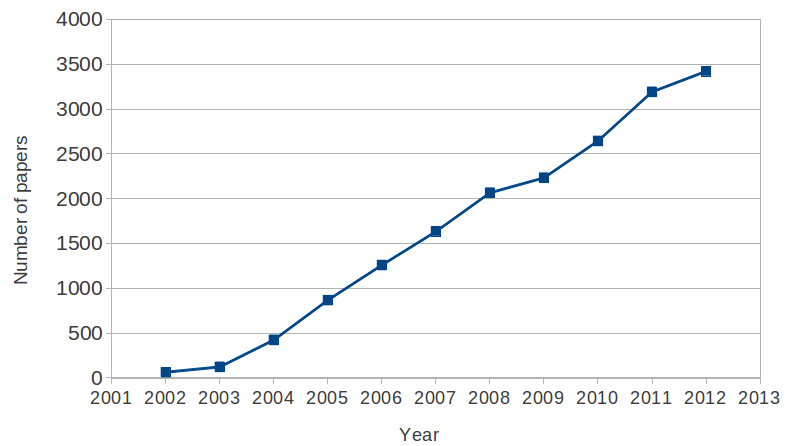
\includegraphics[width=26pc]{gfx/soa/papersYear.png}
\caption{Number of published papers (per year) about SOA (obtained from Scopus database).}
\label{fig:soapapers}
\end{SCfigure}


Service Oriented Architecture (SOA) is a computational
paradigm where agents % users o applications? o agents? - JJ FERGU: cambiado a agents, que es lo más genérico
interact with each other using loosely coupled, coarse-grained, and autonomous components called 
{\em services} \cite{rotem2012soa}. A service is a distributed entity (such as a node, program or
function), used to obtain a result, increasing the integration of heterogeneous
systems (several operating systems, protocols or languages) due to
this multi-platform nature. The service users do not need to know
the language used to implement the service, and they are not
forced to use a specific technology to access that service. For
example, an evolutionary algorithms researcher could have access to a
fitness function made publicly available by another researcher at the
other side of the world without even knowing which programming language
has been used to implement it. % podrías decir la relación que tiene
                               % esto con la ciencia abierta,
                               % resultados reproducibles y demás - JJ - FERGU: lo explico adelante

Also, with the advancement of the Internet, new scientific
communities, based on interoperable and distributed platforms are
emerging. These communities allow scientist to collaborate on their
research, sharing data and remote access to their programs. To achieve
this, they use SOA, obtaining the benefits of the standards it
offers. Users publish and use flexible, interoperable and configurable
services. These services can be created from scratch or by leveraging
existing software \cite{Bechhofer2013ResearchObject}. % un ejemplo!!! - JJ FERGU: esta frase es tuya del paper de la SoCo xD (ejemplo puesto)

\person{Foster} \cite{Foster2005Science} defines the term ``Service Oriented
Science'' as the pursuit of scientific research using distributed and
interoperable networks, being the uniformity of
these interfaces the key to success. Thanks to it, researchers can discover and access
the services without developing specific access for each data source, or
program. %ejemplos!! - JJ FERGU: abajo
Therefore, this paradigm has the potential to increase the
scientific productivity due to these public and distributed services,
and also to increase the data analysis automation in computing. There
are many examples that attempt to boost this paradigm, like Open
Science Grid \cite{Altunay2011OpenScience} and GLOBUS
\cite{Foster2005Globus}.  %citep o cite? - JJ FERGU: era de un paper mío, cambiado
These projects include scientific communities and globally distributed infrastructures that support scientific and integrated applications of different domains.

It is necessary to remark that the technology for implementing services is not the
key challenge in SOA, but to increase the effort to migrate the
existing work and to change the mind of researchers and
practitioners. This is, therefore, one of the aims of this thesis: to  
present to EA researchers the benefits of adopting this paradigm, describing the SOA concepts,
restrictions and methodologies, but also to present the most
used technologies to chose the most adequate one.
%to what? Esto relaciónalo con la tesis, es un capítulo
               %de TU TESIS - JJ FERGU: añadido "one of the aims of this thesis..." y también lo de abajo

In this chapter, the usage of SOA is proposed to facilitate the shortcomings in the EAs presented in the previous chapter: development, integration, standardization and dynamism. First, several concepts to undarsted SOA are explained. Then the most used technologies and methodologies are presented and how can help with the previous shortcomings. After that, the benefits of using SOA in EAs are explained, but also the restrictions of SOA are listed in order to be considered when creating a methodology to develop evolutionary algorithms in this paradigm. 


\section{What is a Service?}
\label{sec:soa:whatis}
\lettrine{A}{} service can be seen as a function call which can be
executed locally or remotely, and which is independent of the
programming language or running platform. As previously said, services have well defined
interfaces, which depends on the desired technology to implement
SOA. That means that the service users do not need to know the
language implementation of the service or the operating system, %esto
                                %ya lo has dicho - JJ FERGU: pongo el "as previously said" lo pongo, pero para que quede claro y se le meta al lector en la cabeza
 and they are not forced to use a specific technology to access to that service.






Figure \ref{fig:soadiagram} shows the basic interaction among
services. First, the \textsc{service provider} exposes the service, publishing
its interface in the \textsc{service broker} (or \textsc{service registry}). The \textsc{service consumer} (or
\textsc{requestor}) finds  a service in the broker to be used and receives its
interface. Then the request is performed by the \textsc{consumer} (which uses or
consumes the service).  

\begin{SCfigure}[20][tb]
\centering
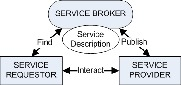
\includegraphics[width=20pc]{gfx/soa/soaDiagram.jpg}
\caption{Service interaction schema. The service pro\-vi\-der publishes a
  service description that is used by the consumer to find and use the
  service.} % no has definido consumer todavía - JJ FERGU: movida la imagen de sitio para definirlo antes
\label{fig:soadiagram}
\end{SCfigure}



According to \person{Valipour} \cite{Valipour09surveysoa}, services must follow these characteristics:

\begin{itemize}
\item {\em Discoverable and Dynamically Bound}: Services must be discoverable. Thanks to the service registry, a service consumer can discover a service to be use at runtime.
\item {\em Self-Contained and Modular}: All functions in SOA are services. This means that every
  component in SOA must be modelled as a service, or as an aggregation of services. The services are well-defined: the interface of the service must be fixed, and it can not change in time, because the consumers or implementations of this interface should be modified with it. Services are, therefore, {\em encapsulated}: only the interface should be used to consume a service.
\item {\em Interoperability}: Consumers do not need to know how the service implementation performs their function, as services behave as a ``black box''. This is, elements such as the programming language or distribution protocol are independent.
\item {\em Loose Coupling}: Services should be designed to need only a few number of well-known dependencies.
\item {\em Location Transparency}: Services must be indistinguishably local or remote, being independent of the protocol to establish the connection.
\item {\em Composability}: Developing applications in SOA means to aggregate different existing services. Services are designed to be {\em re-usable}.
\end{itemize}



Moreover, several implementations of a specific service  can exist (in
one or several machines). The broker can choose which one to use  each
time, or offer another if a service is temporarily
unavailable. Implementations  may also have a different behaviour, so
the researcher can take advantage to create an auto-adaptive algorithm
to select different implementations according to some criteria. % esto
                                % tenías que haberlo hecho para la
                                % tesis!!! - jj FERGU: Experimento realizado y puesto en capítulos siguintes
Figure \ref{fig:servicebasic} shows this special interaction, where two different implementations of an operator interface exist (even using different languages) and the broker has chosen one of them.


The service broker in a SOA can be implemented in several ways and have
different behaviours: for example, the implementations of the services to be used can be
defined in a text file (if the services do not change in execution
time). However, the broker can also assign implementations to
interfaces in an automatic way, or using several rules. For example, in the context of EAs,
to select a better operator if the current one is not working properly.
%to distribute a fitness between several machines activated while the
%algorithm is running. % ¿vas a hacerlo? ¿No? Trata de restringirte a
                      % lo que vas a hacer en la tesis, porque si no
                      % te preguntarán que por qué diablos no lo has
                      % hecho - JJ FERGU: cambiada la frase


\begin{SCfigure}[20][tb]
\centering
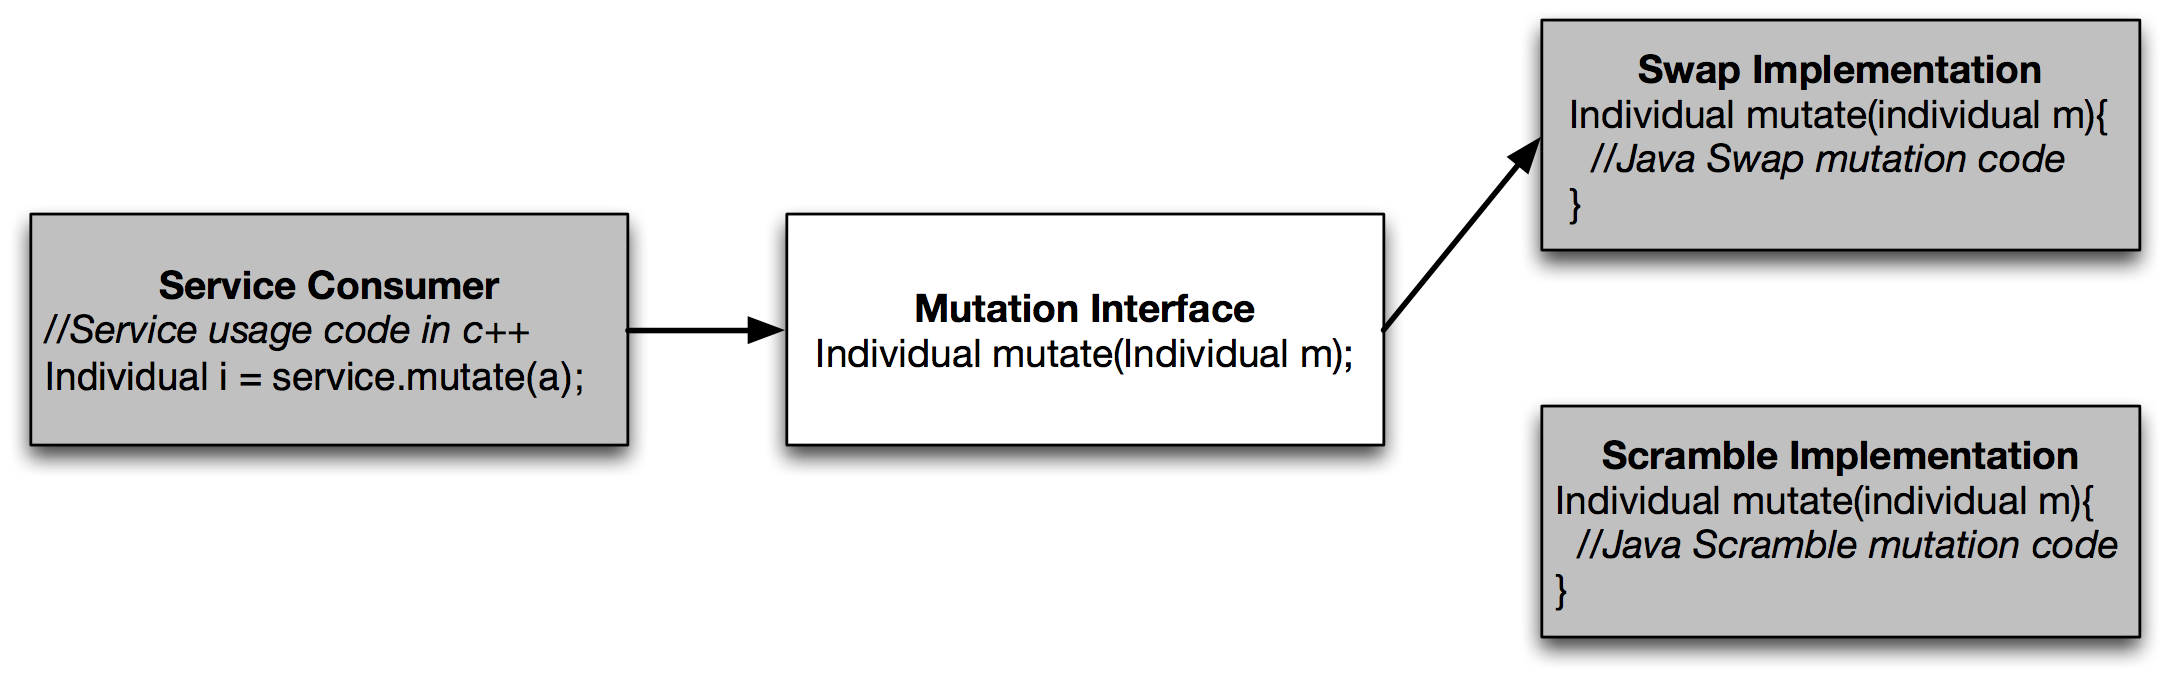
\includegraphics[width=26pc]{gfx/soa/exampleSOA.jpg}
\caption{Example of usage of a service implementation.}
\label{fig:servicebasic}
\end{SCfigure}




An important SOA capability is that it is not focused on a specific
implementation, but offers a set of guidelines to help the
developers. In \cite{Arsanjani2008SOMA} these guidelines and good practices, and also the differences between SOA and Object Oriented
Programming (OOP) are
explained: the main difference between SOA and imperative programming or OOP is the order of service execution. This order is not necessarily static, because the services are designed to be used in a non-established and configurable order. Furthermore, another important difference is that services can be dynamically discovered and used (while in OOP a function/method must be previously known and can not change during execution), being also one of the most important capabilities the (optional) distribution in a network. Finally, in OOP the programming language must be the same for each method call.

\section{Implementation technologies}
\label{chap:soa:implementations}

\lettrine{D}{espite} the fact that the concept of service is independent of the technology used, there exist several ways to use and implement services, being Web Services, REST, \definicion{ebXML}{Electronic Business XML} and \definicion{OSGi}{Open Service Gateway Initiative} the most extended.

\subsection{Web Services}
\label{subsec:soa:ws}
One of most popular services implementations are  \textsc{Web
  Services} \cite{Papazoglou2007SOA}. A web service is a service available over Internet, that uses any standardized XML (eXtended
Meta Language) \cite{XML} messaging system, and it is not tied to any
specific language or operating system \cite{Cerami2002Webservices}.
As SOA proposes, web services should be self-describing (using a
standardized grammar) and self-discoverable. % secciones de un párrafo
                                % no son secciones - JJ FERGU: No, lo de abajo es sub-sub-section, no tiene numeración, pero el resaltado queda bien.

\subsubsection{Messaging system} There are several alternatives to the messaging system, as SOAP or XML-RPC. SOAP (Simple Object Access Protocol) is a standard protocol proposed by the W3C \cite{SOAP}  which  extends the XML remote procedure call (XML-RPC) standard. 
It is a complete and mature protocol that allows performing remote
method calls to distributed routines (services) based on an XML
interface. % SOAP se usa cada vez menos me parece a mi. Podías
           % indicarlo. - JJ FERGU: Cierto, SOAP se está usando menos en web, pero en la empresa. Lo pongo al hablar de REST 

SOAP clients can access objects and methods that are residing in
remote servers, using a standard mechanism that makes  the details of
implementation transparent, such as the programming language of the
routines, the operating system or the platform used by the provider of
the service. % esto lo has repetido por enésima vez - JJ
At the moment, there exist complete implementations of SOAP for Perl, Java, Python, C++ and most modern languages.
Unlike other remote procedure call methods, such as RMI (Remote method invocation, used by the Java language) or XML-RPC, SOAP has two main advantages: it can be used with any programming language, and it can use any type of transport (\definicion{HTTP}{HyperText Transfer Protocol}, \definicion{TCP}{Transmission Control Protocol}, \definicion{SMTP}{Simple Mail Transfer Protocol} and other protocols). In this way, SOAP constitutes a high level protocol, making easy the task of distributing objects among different servers, and avoiding the difficulties derived of defining the message formats, nor the explicit call to remote servers.


\subsubsection{Self-description} The interfaces of the methods of web services that can be accessed are specified by a Web Services Description Language (WSDL) \cite{WSDL}. The WSDL of a web service consists in an XML description of its interface, i.e., it is a file that describes the name of the methods, their parameters (number and type) and their type of response.

\subsubsection{Self-discovery} UDDI ({\em Universal Description, Discovery and Integration}) \cite{UDDI} is a technical specification for describing, discovering and integrating web services \cite{Cerami2002Webservices}. This specification includes APIs for the storage and retrieval of information (also in an standardized XML format).


\subsubsection{Other standardizations} One of the advantages of using
web services % nunca coma entre sujeto y predicado - JJ FERGU: OK
 is that the application stack is growing with the WS-Extensions. That is, the basic specifications of Web Services (such as SOAP) can be extended with transactions, security or messaging, for example. The most used are \cite{Papazoglou2007SOA}:
\begin{itemize}
  \item WS-Addressing  (authentication)
  \item WS-Security , WS-SecureConversation  and WS-Trust  (authorization and secure messaging)
  \item WS-Policy and WS-Metadata Exchange (policy mechanisms for interactions)
  \item WS-Reliable Messaging  and WS-Transaction (add-on mechanisms for the communication channel)
\end{itemize}
% pero todo esto importa lo más mínimo para la tesis? Lo vas a usar? FERGU: explicado después
% No metas rollo por meterlo - JJ
Also, functional extensions, such as WSRF \cite{WSRF}, % qué
                                % significa? - JJ
 allows the discovery, inspection and interaction with stateful resources in standard and interoperable ways. Finally, BPEL ({\em Business Process Execution Language})  \cite{BPEL} is an XML-based language to control the invocation of different Web services with added business logic to help large-scale programming.

The main advantage of using Web Services in research is their public discovering and usage, thanks to the security extensions. Several studies about e-science taking advantage of web services can be found in bibliography \cite{Oinn04Taverna,davidson08workflows,Ludascher06Kepler,Perera06workflows}.

\subsection{REST}
\textsc{Representational State Transfer} (REST)\footnote{\url{http://en.wikipedia.org/wiki/Representational_state_transfer}} is an al\-ter\-na\-ti\-ve me\-thod to build web services.
This architectural style % no es una tecnología, es una convención!!! - JJ FERGU: cambiado a architectural style
was proposed and defined by \person{Fielding} in \cite{Fielding2002}.

In a REST-style architecture, a client sends requests to the server, who processes them and returns responses to the client.
Requests and responses represent resources that can be addressed by a Uniform resource identifier (URI). Usually, resources are documents or programs the client need to access.

REST usually works over the HTTP protocol. However it can be based on other protocols that provide the appropriate mechanisms to send requests and return responses.

In a REST environment, while servers are not concerned with the client state, clients only take about their own state and how to address resources on the server using URIs. Moreover, clients can cache responses to improve performance.
As the client-server communication is stateless, servers are simpler and more scalable. 
Taking this into account, if the REST interface is not altered, servers and clients can be modified independently.
Finally, servers can customize the functionality of the clients by sending their logic (code) to be executed.


REST web services are simple and lightweight (as no extra XML markup
is needed), their message format is readable by humans, they are easy
to build, and finally, developments achieve a high performance
\cite{Daigneau2011}. % podías citar el trabajo de Pedro SOAP vs. REST
                     % - JJ
The main differentiating factor is that Web Services using SOAP tend to be operation-based, while REST services are resource-based. This is one of the reasons REST is replacing SOAP on the web \cite{Mason11REST}. %FERGU: puesto lo de que se usa menos en la web

\subsection{ebXML}
ebXML defines a set of standards that allows the enterprises negotiate their products through the Internet. It is based on a well-defined documents interchange using a contract-based approach \cite{Patil03ebxmlVsWS}, providing a specification for messaging, registry/repositories and business processes description, and unlike other approaches, it is an horizontal standard (it is not oriented towards a specific industry sector). On the contrary, Web Services expose any kind of applications to the Web, so anyone can call them (service approach). Another significant difference between Web Services and ebXML is that the former is based on BPEL, which can only describe the scenario inside a company, due to it has not all the information about the services being orchestrated, while the latter can be used to model a global choreography among several companies. Due to this, and because it is mainly focused to commercial and business processes, this technology is not going to be addressed in this thesis.

\subsection{OSGi}
\label{subsec:soa:osgi}
OSGi was proposed by a consortium of more than
eighty companies in order to develop an infrastructure for the
deployment of services in heterogeneous network of devices, mainly
oriented to domotics \cite{GarciaSanchez2013Gateway,GarciaContext11}. Nowadays it defines a
specification for a SOA for virtual
machines (VMs). It provides very desirable features, like
packet abstraction, life-cycle management, packaging or versioning, % qué significa todo esto? - JJ FERGU: Añado ref
allowing a significant reduction of the building, support and deployment
complexity of the applications. These features can be useful in the field of EAs, as suggested by \person{Wagner \etal} \cite{WagnerPlugins07}.

OSGi technology allows dynamic discovery of new components (or services), to increase the collaboration and to minimize and manage the coupling
among modules. Moreover, the
OSGi Alliance has developed several standard component interfaces for
common usage patterns, like HTTP servers, configuration, logs, security,
management or XML management among others, whose implementations can
be obtained by third-parties. %Nowadays there are some challenges
% nowadays y citas un trabajo del 2008? - JJ
%in the OSGi development \cite{Kriens2008OsgiChallenges}, but they only
%affect the creation of very complex applications. % y, como dicen en
                                % mi pueblo, los algoritmos evolutivos
                                % son más simples que paja de habas? - JJ
                                %FERGU: meh, lo comento todo, tampoco era muy interesante

These advantages are not so
                               costly as can be thought: on one hand the OSGi
                                framework can be implemented in a
                                {\em jar} file\footnote{A jar file is
                                a file that groups some compiled Java
                                files.} of about 300KB, and on the other hand, and differing from
                                the normal usage of Java, each
                                class pre-charges only the other
                                classes it needs, not all. Also it is
                                non-intrusive: the code to be
                                executed in OSGi can be executed
                                without it. Finally, from its
                                specification in 1998 has been widely
                                used as base in big projects: the
                                Eclipse \definicion{IDE}{Integrated Development
                                Environment} is built over OSGi, and
                                also big application servers
                               (Glassfish\footnote{\url{http://glassfish.java.net}} 
                               or IBM Websphere \footnote{\url{http://www.ibm.com/software/websphere/}}) or
                               residential gateways
                               \cite{GarciaSanchez2013Gateway}, among other
                               examples. 



%\subsubsection{Distribution}
In OSGi all services can be distributed using the OSGi
features, simply setting which service is distributable and which is
the distribution technology that provides service discovering and data
transmission.   % so what? - JJ % ¿Esto es relevante? - JJ FERGU: TODO sí, esto es MUY relevante, lo uso en la tesis, pero antes es que era una sección más grande. Pregunta: menciono aquí que  voy a usar OSGi en mi tesis o en el capítulo Osgiliath? (ahora está en ese capítulo)

\section{Methodologies for developing SOA}
\label{chap:soa:methodologies}
\lettrine{R}{egardless} of the chosen SOA framework, the processes % business? no estamos hablando de algoritmos - JJ FERGU: sí, es que a veces se les llama así, pero lo quito para no liar
 of the platform must be analysed and modelled. So it is necessary to use a consistent and well-defined methodology to design a model based on a machine-readable description \cite{Garcia09UMM}. {\em Business-Centric Methodology (BCM) for Enterprise Agility and Interoperability} \cite{Oasis03BCM} is a roadmap for the development and implementation of procedures to create effective, efficient, and sustainable interoperability mechanisms. It has been developed by OASIS, the same consortium that created BPEL or UDDI, among others, and it is complementary to other existing architectures and technologies designed to build business oriented services, like ebXML or Web Services. BCM is formed by a set of model layers with a step-guide process, and an information pyramid to align the semantic information of partners. This allows the participation of business experts and the creation of a very large documentation repository. Nevertheless, this methodology has some disadvantages: it has a very large learning curve and it is not very extended yet. 



{\em \definicion{UN/CEFACTs}{United Nations Center for Trade
    Facilitation and Electronic Business} Modelling Methodology (UMM)}
\cite{Hofreiter06UMM} is an approach to model the business services
that each partner must provide in order to perform a
\definicion{B2B}{Business to Business} collaboration. It has a
complete meta-model about business processes and business information,
including a process analysis methodology. It is interesting to show
that UMM provides and supports components to capture the knowledge
about the business processes, and that it is independent of the
underlying implementation technology (ebXML, Web Services,
\definicion{CORBA}{Common Object Request Broker Architecture} or
\definicion{EDI}{Electronic data interchange}). Furthermore, because
UMM extends \definicion{UML}{Universal Modelling Language}, we could
say that this methodology is more easily adaptable, due to the high
development, acceptance and maturity of UML \cite{Garcia09UMM}. In
fact, a survey of B2B modelling languages show that UMM is the most
complete approach \cite{Folmer08b2b}. 

Finally, {\em SOMA} (Service Oriented Modelling and Architecture)
\cite{Arsanjani2008SOMA} is an architecture proposed by IBM to model
service oriented processes. It lets the identification, specification
and implementation of  the services, flows and components inside the SOA paradigm. To achieve
this tasks, it proposes a top-down modelling oriented to
intra-enterprise services (service-oriented instead of
business-oriented). It is more agile than the previous ones
and it is not focused in enterprise environments. 

%Pero ¿esto lo vas a usar? ¿Le interesa lo más
                    %mínimo al revisor y/o tribunal? - JJ FERGU: si, cambiado el capitulo siguiente




%%%%%%%%%%%%%%BENEFICIOS DE USAR SOA EN EAs
\section{Benefits of using SOA in Evolutionary Algorithms Area}
\label{sec:soa:benefitsofsoa}

% de hecho, no has incluido el trabajo principal en el área, que tienes que conocer, y además es de Enrique Alba:http://onlinelibrary.wiley.com/doi/10.1002/9780470411353.ch25/summary Tiene una versión en español - JJ FERGU: no lo conocía, añadido

\lettrine{S}{OA} has been previously used in the EA area. \person{Garc\'ia-Nieto \etal} proposed {\em Remote Optimization Service}  \cite{ROSGarcia08}, a client/server environment for launching different algorithms programmed in several languages. Although it uses XML and DTD to define inputs and outputs of the services, only the whole algorithm is exposed as a service. Also, this system does not allow dynamic discovering or combination of available operators.

Web Services have been used in the grid area for optimization
problems, as can be seen in the works of
\cite{grid1,grid2,grid3,grid5}, where services are defined using WSDL
interfaces and other transmission mechanisms (such as Remote Procedure
Call \cite{grid6,grid7}). 

Although EAs are executed in grids
\cite{grid8,grid4,grid10}), no information about how to design these
services for EAs has been provided in previous works.  % estás
                                % diciendo que no hay una metodología
                                % para diseñar estos servicios y eso
                                % es gordo, porque entonces tienes que
                                % hacerlo tú - JJ FERGU: Hecha la metodología en el capítulo siguiente :)

In the previous chapter several shortcomings % y dale - JJ FERGU: cambiado a shortcomings
 in the Evolutionary Algorithms area were presented, such as the new trends of
 distributed programming where nodes enter and exit in runtime, or the
 incompatibility between frameworks, for example. All these facts
 motivate the creation of a proper way to define services for evolutionary algorithms. The elements that combine an EA are candidate to be designed as services, as they can behave as input/output functions. Also, SOA solve the problems previously addressed: 



\begin{itemize}
\item {\em Development}: there exist several methodologies to model and design services. Also, as services are re-usable, they can be combined in different ways to create the different types of EAs. Moreover, existing technologies, also facilitate the development, using techniques such as versioning, packaging or life-cycle control.
\item {\em Integration}: Services are independent of the programming language. For example, services implemented in Java may use services implemented in C++ and vice-versa. Also, services allow distribution transparency: it is not mandatory to use a specific library for the distribution, or modify the code to adapt the existing operators. Existing EA frameworks could also be adapted to be accessed as services, providing their interfaces. 
\item {\em Standardization}: Interfaces of services use public
  standards (such as WSDL \cite{WSDL} or OSGi \cite{OSGI}). The
  service interfaces for EAs should be abstract enough to avoid their
  modification. Furthermore, as \person{Foster} claims
  \cite{Foster2005Science}, SOA is the key to develop Open Science. 
\item {\em Dynamism}: Services are not aware of the order of execution, so this paradigm can fit with new parallel approaches for EAs, where the control of the nodes is not centralized. Also, SOA provides techniques for automatic discovering of services. For example, new operators in different nodes can be bound and used during the run of an algorithm. Also, there should be easy to add and remove elements to achieve self-adaptive mechanisms.
\end{itemize} 


% no te repitas. Eso ya lo has dicho
                        % antes. Suena a que estás metiendo morralla
                        % por rellenar - JJ FERGU: Borrado ENTERO y reescrito arriba. Tambíen borrado abajo otros párrafos que me repetía mucho

% vaya, aquí lo dices, pero antes no - JJ FERGU: (era lo de open science) sí, está dicho arriba (y citado)







%%%%%%%%%%%%%%%%%%%%%%RESTRICCIONES EN SOA PARA DISEÑAR EAs
\section{Restrictions in SOA design for EAs}
\label{sec:soa:restrictions}
To allow these benefits the services for EAs should match with the next technological
restrictions: % ¿por qué? ¡Justifícalo todo! - JJ FERGU: Cambiada la primera frase para justificar lo siguiente

\begin{itemize}
\item The services can be dynamically bound to change the needed EA aspects. %bind o be bound - JJ FERGU: arreglado
\item The source code of  the basic EA services should not be  re-written or re-compiled to achieve this task. That means that the design must be as abstract as possible. % seriously? must not been? - JJ FERGU: arreglao
\item New services can be added in execution time. 
\item No specific source code for a distribution must added, neither  the existing source code of the services should be modified for this purpose (that is, changing distribution libraries must not add extra code in existing services). 
\end{itemize}


%In previous chapter we also presented the advantages of using SOA in Evolutionary Algorithms area: firstly, SOA fits with the genericity advantages in the development of software for EAs \cite{GENERICITY05} and adds new features, like language independence and  distribution mechanisms. It also allows the addition and removal of services in execution time without altering the general execution of the algorithm (that is, it is not mandatory to stop it or to add extra code to support new operators). This issue increases the interoperability between different software elements. Moreover, this allows easy code distribution: SOA does not require the use of a concrete implementation or library.
%FERGU: comentado este párrafo, que me repito (antes estaba en otro capítulo)






One of the main restrictions in SOA, % ¿SOA o SOAs? será "a SOA" o
                                % "SOAs", ¿no? - Jj FERGU: no, SOA es una metodología de diseño
 apart from focusing on the development of abstract services, is the
 stateless and un-ordered nature of services. Therefore, services must follow the next guidelines.
 % ¿Puede estar esto relacionado con
                                % programación funcional? Podías mirar
                                % y citar los papers de Albert al
                                % respecto - JJ FERGU: no, no está relacionado (pero ya cito los papers de Albert antes)

First, as services are unaware of each other, there should not be global
variables in any part of the code. Services are listening, and waiting
to be executed. For example, a fitness service with a counter that is
increased each time is called (to stop the algorithm if a limit is
reached, for example). If several (and different) algorithms were
working in parallel, and calling this function concurrently, the
counter could not distinguish between algorithms, giving erroneous
results. However, a service that maintains some kind of state is
allowed, for example, a statistics service that reads events from all
the algorithms being executed at the same time, but this should be
managed to avoid errors. % ¿en qué quedamos entonces? ¿Se permite o no
                         % se permite? - JJ

Also, a service should not be distinguishable from local or remote
running in other node in the network. % es la 5ª vez que dices esto - JJ FERGU: sí, pero ahora lo enlazo con los EAs
Every stage in the algorithm should be treated as a service to be
executed in local or in remote, even the {\em Population} or the {\em
  Parameters}. Mechanisms to ensure the correct data-sharing should be
provided. Also, many implementations of the same service could exist
at the same time (different implementations of {\em Crossover}, for
example) and they should be correctly managed and used. % pero ¿las va a
                                % haber? ¿Vas a usar estas
                                % características? - JJ FERGU: sí, las va a haber y lo voy a poner en el experimento (aunque estaba descrito en siguientes capítulos)

Moreover, a service is always a request-response function. For
example, the fitness calculation should not be a method of the {\em
  Individual} implementation, but a function that receives a list of
individuals and returns a list of the calculated fitness of that
individuals. This allow, for example, remote fitness calculation and
distributed load balancing, impossible to perform if the fitness is a
method of the {\em Individual} class. % Esto ya se hizo cuando
                                % diseñamos los Evolving Objects,
                                % podías citarlo - JJ FERGU: 

Thinking as abstract as possible requires to separate concepts such as
the order of recombination, and the crossover itself. Usually, after
parent selection, individuals are crossed in order. However, if we
need a different mechanism for mating (for example, using more than
two parents, or parent selected several times) a duplication of effort
is needed. That is the reason to separate the concept {\em
  recombine} from {\em crossover} (and also, following the top-down
design proposed in SOMA).  % ¿Esto es lo único que estás usando del
                           % SOMA? - JJ FERGU: no he cambiado el capítulo siguiente a saco

Finally, no assumptions should be taken about services previously
executed or being executed next. For example, the {\em Mutation} 
service could be applied before the {\em Recombination} or the fitness could be calculated in the middle of the generation. %For example, services to implement {\em
  %Recombinator} or {\em Mutator} should return the individuals with
%their fitness already calculated. % ¿Por qué? ¿Eso no implica que el
                                % mutador tiene que saber que existe
                                % otro servicio que calcula el
                                % fitness? Además, en la práctica el
                                % mutador no necesita el fitness (casi
                                % nunca)- JJ FERGU: cierto, quitado
Usually this step is performed in
the last stage of the generation, but if we require the individuals
for other tasks: for example, a Local Search or a statistics collector
to guide the algorithm. % if we require, ¿qué? - JJ FERGU: ejemplo puesto

\section{Conclusions}

\lettrine{E}{ven} as SOA is used extensively in software development area, it is
not widely accepted in the main EA software, as the survey of frameworks by \person{Parejo et al.}, presented in Section \ref{chap:distributed:conclusiones} claim. % pruébalo - JJ FERGU: Probado con la referencia al survey
The authors of these frameworks should improve their frameworks adding SOA technologies in
order to facilitate the communication and integration among them, without
 duplication of effort to re-program all the EA elements, and therefore, saving time. 
 Therefore, the benefits of using SOA in development, integration, standardization 
 and dynamism (presented in Section \ref{sec:soa:benefitsofsoa}) could be applied.
  % ¿y qué se conseguiría con eso? - JJ FERGU: reescrito y añadidas cosas
 Although all the approaches described Section \ref{sec:distributed:parallel} are focused
 on the implementation of distributed EAs, the abstraction level of
 each alternative can be quite different, as shown in Figure
 \ref{fig:soagrid}.  As SOA is a paradigm and not a technology,
 areas such as Evolutionary Robotics, or EA classic frameworks can use
 SOA to be designed and developed. Implementation technologies, such
 as Web Services, can fill the gap between SOA (abstract) and grid
 (infrastructure) where interfaces are designed using SOA principles
 (dynamism, visibility, loose-coupling and heterogeneity). Finally,
 cloud computing can be seen as a combination that extends SOA adding
 the scalability of the grid, ad suggested by \person{Jamil}
 \cite{SOALIB}. % y esto es interesante porque.. - JJ


\begin{SCfigure}[20][tb]
\centering
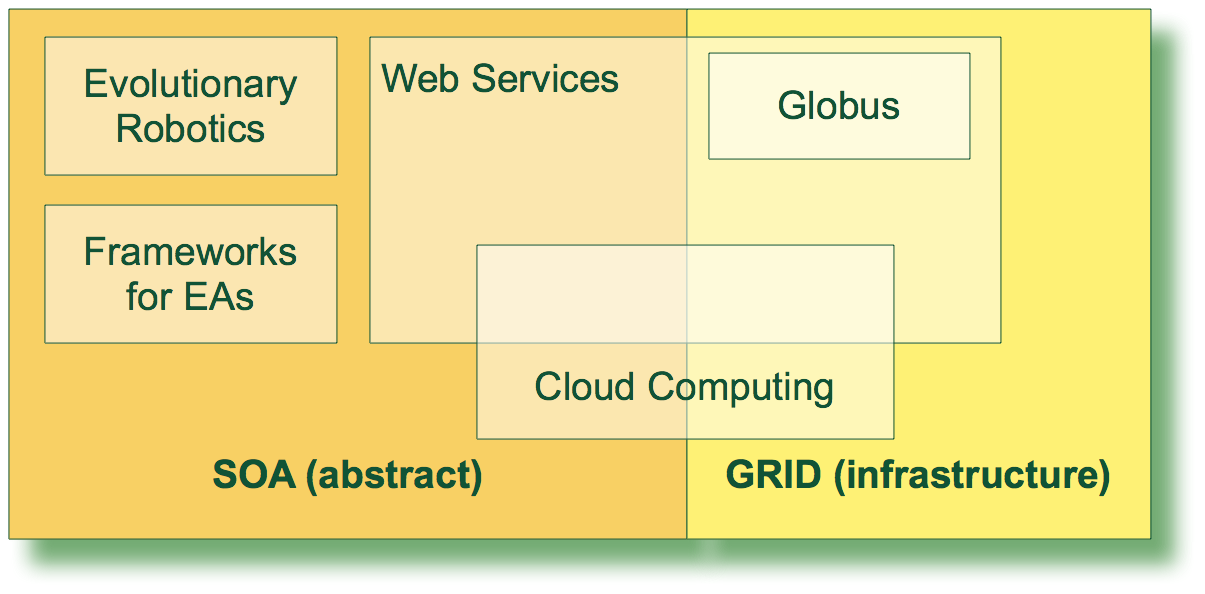
\includegraphics[width=26pc]{gfx/soa/soagrid.png}
\caption{SOA as abstract paradigm to develop EAs in different
  areas. %¿to develop qué? ¿o to be developed? - JJ FERGU: arreglado
 Using specific technologies such as Web Services allows grid integration. This figure has been updated from the one presented in \cite{SOALIB}.}
\label{fig:soagrid}
\end{SCfigure}
In this thesis the SOMA guidelines (identification, specification and
realization of the services, flows and components) are going to be used, because it is the
% Esto tienes que decirlo donde estés hablando de SOMA. - JJ FERGU: puesto
methodology more flexible and less focused on commercial
purposes. Next chapter will present a methodology to use the design principles of SOA for
developing services for EAs. Then, in later chapters, a specific SOA technology will be
used to develop an implementation of a service oriented architecture
for EAs.
}{\myChapter{Service Oriented Architecture: technologies and restrictions for designing services for EAs}\label{chap:soa}}
\ifthenelse{\equal{\value{IncluyeCapitulo}}{2}}{\myChapter{A Service Oriented Architecture for EAs}\label{chap:soaea}
\minitoc\mtcskip
\vfill
\lettrine{S}{OA}s provide a good set of solutions to solve some of the
problems in the EA area, such as the lack of integration,
standardization and dynamism control. It also allows ease of
development in dynamic, distributed and heterogeneous systems. % ¿quién
                                % ha dicho que eso es un problema? - JJ
 However, several restrictions must be taken into account. In this
 chapter, we present the existent restrictions in the EA design,
 according to \person{Gagn\'e and Parizeau} \cite{GENERICITY05}. Also,
 the restrictions in SOA design (such as the unordered execution or
 distribution transparency) are explained to perform % are explained
                                % to perform? - Jj
 a good design of services for EAs. All these requirements are used to explain how the different elements of an EA must be designed. % cita el capítulo anterior - JJ

SOMA methodology \cite{Arsanjani2008SOMA}, explained in previous chapter, establishes that the phases of the SOA design are {\em identification}, {\em specification} and {\em realization} of the services and flows. In this chapter, we identify the services that compose an EA and specify some of their possible behaviours. The realization of the designed services will be explained, using an specific technology, in the next chapter. 

For a better understanding, a complete example of development of an EA
is explained. This example is modified to show how to convert an
algorithm to another, dynamic operator changing, load balancing and
even intelligent aggregation of operators.

% ¿Este capítulo es ciencia? ¿Tecnología? ¿Puro desarrollo? Deja bien
% clara la aportación de este artículo, aparte de la obvia
% implementación. ¿Has hecho una abstracción de los algoritmos
% genéticos? ¿Un survey de técnicas usadas? - JJ

\section{Design of services for Evolutionary Algorithms}

This section shows the restrictions for designing EAs (from the point of view of a EA practitioner) and services (from the SOA area expertise).

\subsection{Restrictions in EAs design}

%%%PONER LO GENERICITY DE PAPAZOGLOU

In Chapter \ref{chap:distributedEAs} the restrictions that \person{Gagn{\'e} and Parizeau} proposed to qualify a framework for EAs were presented. This criteria should be used to design the services for EAs.

%hala, repitiendo lo que dices en el capítulo anterior. Pa matarte. - JJ
\begin{itemize}
\item Generic Representation: the structure of the individuals must no
  Therefore, services must accept {\em Individuals} interfaces as
  inputs, not concrete implementations (such as vectors or lists). % ¿Por qué las mayúsculas? - JJ
\item Generic Fitness: In the case of using SOA, the fitness must be a separate service.
\item Generic Evolutionary Model: An example would be an implementation called {\em Evolutionary Algorithm} with all the steps common to all EAs and with independence of the implementations of these steps.
\end{itemize}
All these characteristics of genericity for the design of an EAs should be taken into account when designing services for EAs. However, requirements are aligned with the requirements for designing services, as explained next.

\subsection{Restrictions in SOA design}

SOA follows these lines of genericity presented in previous sub-section, and can also extend them:
\begin{itemize}
\item Genericity in the service interfaces: service interfaces are established to create new implementations. Furthermore, these interfaces must be abstract enough to avoid their modification.
\item Programming language independence: for example, services implemented in Java can use services implemented in C++ and vice-versa.
\item Distribution transparency: it is not mandatory to use a specific library for the distribution, or modify the code to adapt the existing operators.
\item Flexibility: easy to add and remove elements to use the self-adaptation or other mechanisms.
\end{itemize}

As explained in previous chapter, when developing within a SOA, \person{Papazoglou \etal} \cite{Papazoglou2007SOA} established that the services must be: 
\begin{itemize}
\item Abstract: many different implementations can use the same interface.
\item Well-defined: the interface of the service must be fixed, and it can not change in time, because the consumers or implementations of this interface should be modified with it.
\item Encapsulated: services can use other services, but only the interface should be used to consume a service.
\item Reusable: services should be designed to be used by as many applications as possible. 
\end{itemize}

One of the main restrictions in SOA, % ¿SOA o SOAs? será "a SOA" o
                                % "SOAs", ¿no? - Jj
 apart from focusing in the development of abstract services, is the
 stateless nature of services. Therefore, in SOA the services design
 must follow several guidelines. % ¿Puede estar esto relacionado con
                                % programación funcional? Podías mirar
                                % y citar los papers de Albert al
                                % respecto - JJ

First, as services are unaware of each other, there must not be global
variables in any part of the code. Services are listening, and waiting
to be executed. For example, a fitness service with a counter that is
increased each time is called (to stop the algorithm if a limit is
reached, for example). If several (and different) algorithms are
working in parallel, and calling this function at the same time the
counter would not distinguish between algorithms, giving erroneous
results. However, a service that maintains some kind of state is
allowed, for example, a statistic service that read events from all
the algorithms being executed at the same time, but this should be
managed to avoid errors. % ¿en qué quedamos entonces? ¿Se permite o no
                         % se permite? - JJ

Also, a service must not be distinguishable from local or remote
running in other node in the network. % es la 5ª vez que dices esto - JJ
Every stage in the algorithm should be treated as a service to be
executed in local or in remote, even the {\em Population} or the {\em
  Parameters}. Mechanisms to ensure the correct data-sharing should be
provided. Also, many implementations of the same service could exist
at the same time (different implementations of {\em Crossover}, for
example) and it should be correctly managed and used. % pero ¿las va a
                                % haber? ¿Vas a usar estas
                                % características? - JJ

Moreover, a service is always a request-response function. For
example, the fitness calculation must not be a method of the {\em
  Individual} implementation, but a function that receives a list of
individuals and returns a list of the calculated fitness of that
individuals. This allow things such as remote fitness calculation and
distributed load balancing, impossible to perform if the fitness is a
method of the {\em Individual} class. % Esto ya se hizo cuando
                                % diseñamos los Evolving Objects,
                                % podías citarlo - JJ 

Thinking as abstractly as possible requires separate concepts such the order of recombination, and the crossover itself. Usually, after parent selection, individuals are crossed in order. However, if we need a different mechanism for mating (for example, using more than two parents, or parent selected several times) a duplication of effort is needed. That is the reason we should separate the concept {\em recombine} from {\em crossover} (and also, following the top-down design proposed in SOMA). 

Finally, we must not make assumptions about services previously executed or being executed next. For example, services such {\em Recombinator} or {\em Mutator} should return the individuals with their fitness already calculated. Usually this step is performed in the last stage of the generation, but if we require the individuals for other tasks: for example, a Local Search or a statistics collector to guide the algorithm.

\subsection{Other technological restrictions}

In previous chapter we also presented the advantages of using SOA in Evolutionary Algorithms area: firstly, SOA fits with the genericity advantages in the development of software for EAs \cite{GENERICITY05} and adds new features, like language independence and  distribution mechanisms. It also allows the addition and removal of services in execution time without altering the general execution of the algorithm (that is, it is not mandatory to stop it or to add extra code to support new operators). This issue increases the interoperability between different software elements. Moreover, this allows easy code distribution: SOA does not require the use of a concrete implementation or library.

The services developed must match with the next technological restrictions:
\begin{itemize}
\item These services can dynamically bound to change the needed EA aspects. 
\item The source code of  the basic EA services must not been re-written or re-compiled to achieve this task. 
\item New services can be added in execution time. 
\item No specific source code for a distribution must added, neither the existing source code of the services should be modified for this purpose (that is, changing distribution libraries must not add extra code in existing services).
\end{itemize}

\subsection{Designing the services}

Taking into account the previous restrictions a possible way for designing services for EAs is shown: 

\begin{itemize}
\item Individual representation. Almost all services in an EA (like mutation or selection) will accept individuals as input data and produce/modify these individuals. Due to many kind of individuals may exist, the operators should be as abstract as possible to operate properly.
\item Fitness evaluation. Each problem should implement an interface of the fitness service that receives the individual, allowing the distribution of this service (instead of being a method in the {\em individual} class, for example). However, to be more flexible, the {\em fitness service} must receive a list of at least one individual, to facilitate the parallelism.
\item Definition or addition of every type of operator. Thanks to the loose coupling of services, several crossover or mutation implementations can be created. Moreover, new operators can be added in execution time, without re-compiling the existing ones, or combining them according to several parameters, for example.
\item Adaptation of the evolutionary model. The user can manually select the services to be combined to create a Genetic Algorithm or an Evolution Strategy, for example.
\item Dynamic adaptation of the parameters. Parameters can also be a service, thus the EA developer obtains two advantages: it is not mandatory to distribute the parameters among all services, and also they can be dynamically modified in execution time from an external service, facilitating self-adaptation \cite{eiben2005shared}.
\item Flexible output mechanisms. The developers do not need skills in GUIs (Graphical User Interfaces) or logs programming, because as this kind of services are not coupled to the operators, they can access their information without any modification in the operators.
\end{itemize}






As previously stated, the 
fitness should not be calculated within a method of an {\em Individual} class. To be less
coupled, it should be implemented an an external service that receives a list of individuals (facilitating the load balancing). That way, the service is as abstract as possible. Also the parameters should be
a service for the same reason, allowing the possibility of performing
experiments related to the parameter control or tuning \cite{ParameterControlEiben07} in an efficient way
(being separated from the code of the existing operators). Services such as the
{\em recombinator} or the {\em mutator} should not receive one or two
individuals, since not all EAs have the same behaviour. They should receive a
list of individuals to be crossed or mutated each generation. On the other way,
{\em population} should not be a list of individuals: it should be a service
to access the individuals and allow the variation of its structure (for example, a change
from an unique list population to a cellular model) without
affecting  the rest of the pieces of the algorithm. So, other services
external to the EA could consult the {\em population} state and act
accordingly to some rules. 

Using the previous indications as a base, SOA-EA has been created. SOA-EA is an
abstract architecture to develop service oriented EAs, independently
of the technology to be used. Table \ref{tab:reasons} shows some reasons to
migrate to SOA and how services in SOA-EA should be designed. 





\begin{SCtable}[][t]

\resizebox{11cm}{!}{
\begin{tabular}{p{2cm}p{2.5cm}p{3cm}p{7cm}}
%\begin{tabular}{llll}
%\noalign{\smallskip}\hline\noalign{\smallskip}
\hline
\rowcolor{colorCorporativoSuave}\textbf{Element} & \textbf{Current EAs development} & \textbf{Using SOA} & \textbf{Reason to migrate} \\
\hline \hline
%\rowcolor{colorCorporativoMasSuave}\noalign{\smallskip}\hline\noalign{\smallskip}
\rowcolor{colorCorporativoMasSuave}{\em Programming language} & Just one for all elements of the algorithm & Any & Services are independent of the programming language. Only the interface is required to use services  \\\hline
\rowcolor{colorCorporativoSuave}{\em Operators} & Methods or functions & Services & Services allow the selection of a specific implementation during the algorithm execution, and also different programming languages or distribution models\\\hline
\rowcolor{colorCorporativoMasSuave}{\em Operators behaviour} & Methods applied to a single individual & Service that receive individual lists  & It allows  load balancing and distribution, and also to modify the operators in execution time\\\hline
\rowcolor{colorCorporativoSuave}{\em Operator selection} & Modifying the source code & In a flexible way outside the source code & It is not mandatory to recompile the source code to integrate new operators \\\hline
\rowcolor{colorCorporativoMasSuave}{\em Fitness} & Method that evaluates an individual & Service that evaluates an individual list & It allows the distribution, load balancing and addition of new fitness calculators in real time \\\hline
\rowcolor{colorCorporativoSuave}{\em Population} & Array or individual list & Population service & It allows to change the population type and topography, by selecting the service implementation \\\hline
\rowcolor{colorCorporativoMasSuave}{\em Self-adaptation} & Modifying source code for a specific experiment & Self-adapting service that selects specific operator implementations & It does not modify the created services and brings more flexibility in the dynamic adaptation \\\hline
\rowcolor{colorCorporativoSuave}{\em Distribution} & Libraries like MPI & SOA mechanisms & SOA technologies allow changing the transmission protocol and using extra technologies without adding extra code\\
%\noalign{\smallskip}\hline
\hline
\end{tabular}
}
\caption{Summary of migration from traditional EA programming to SOA}

\label{tab:reasons}
\end{SCtable}

\section{Example of creating a service oriented evolutionary algorithm}
This section justifies the design of SOA-EA and the steps to create services within it. 
\subsection{Implementing a basic Genetic Algorithm}

As  stated above, a basic EA is formed by several steps. These steps are common to every EA, so this part must be fixed  to allow the creation of services as abstract as possible. The differences between two EAs are in the operators, selectors or individual representation (as suggested by \person{Eiben and Smit} \cite{ParameterTuningEiben2011}). Therefore, to accomplish with the genericity presented in the previous section, the parameters and operators must be added dynamically. This is done with the SOA service binding. Users can specify the operators they need in several ways, for example, in a configuration file, or in an intelligent manner (an algorithm). It is important to remark that these ``pieces'' do not need to be modified and compiled again, because the loose coupling and the dynamic binding of SOA. Without SOA this behaviour is very difficult to achieve or maintain.


\begin{SCfigure}[20][htb]
\centering
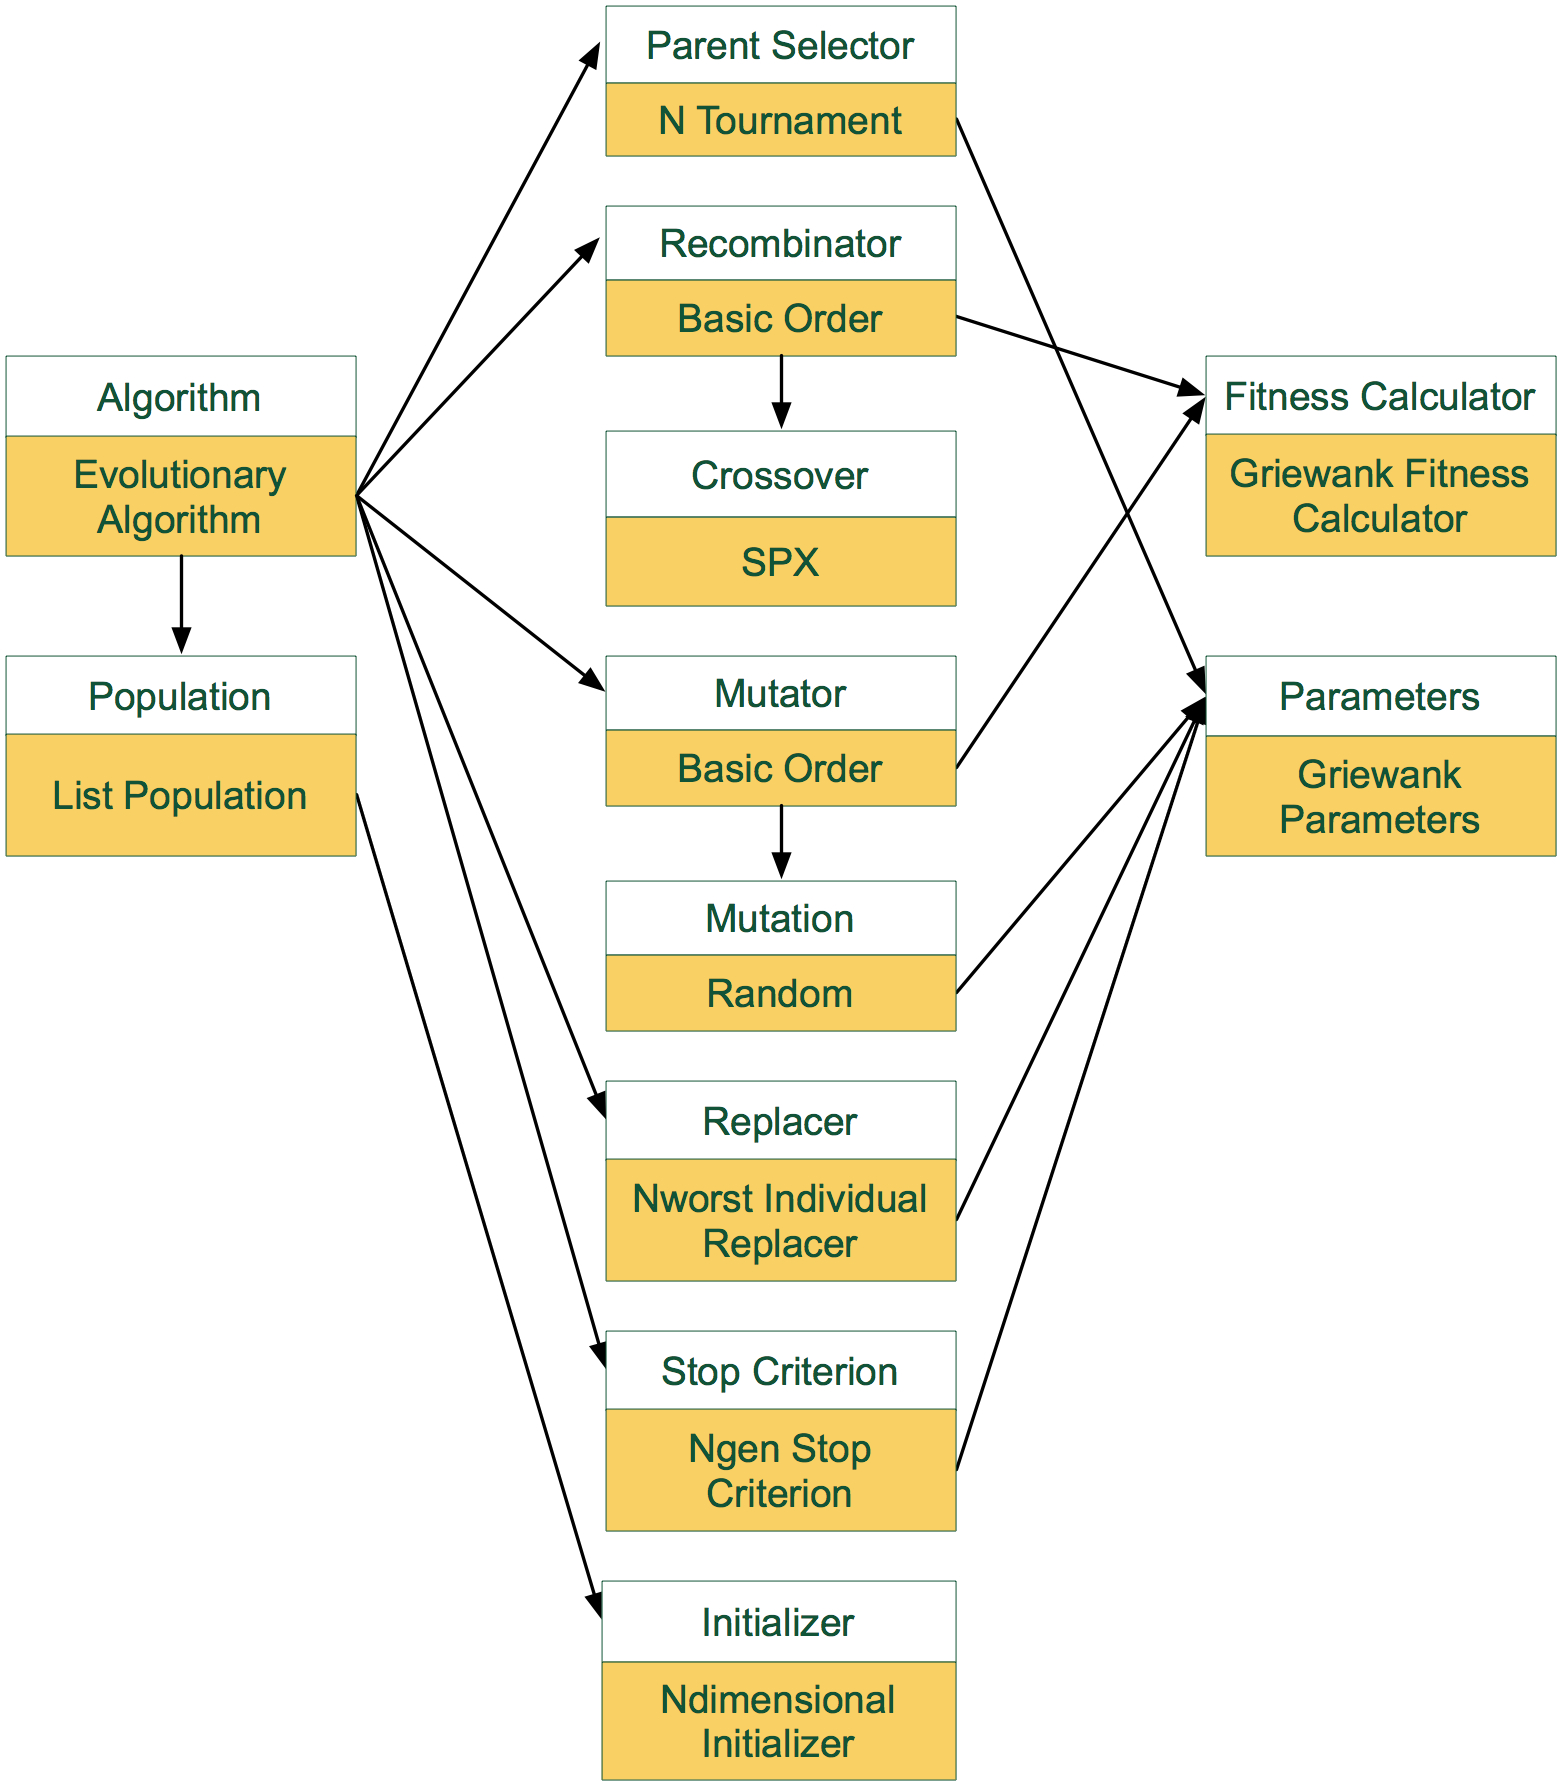
\includegraphics[width=10cm]{gfx/soaea/basicga.jpg}
\caption{Basic genetic algorithm. White blocks are interfaces and orange blocks are implementations. In this case, we are using specific implementations to solve the Griewank function problem.}
\label{BASICGAEXAMPLE}
\end{SCfigure}





Figure \ref{BASICGAEXAMPLE} shows a complete service oriented genetic algorithm, taking into account the proposed ideas. In this figure (and in the following ones) white blocks are the service interfaces. Orange blocks are specific implementations of these interfaces (that is, the source-code of the service), and  arrows indicate how a service implementation can make use of other services via their interface. For example, almost all implementations access to the {\em Parameters} service using its interface. Service implementations (orange blocks) can be selected in a configuration file or be automatically bound when they are available (among other options).

 The change from a problem instance to another is quite simple. It is only necessary to notify the algorithm a change in the implementation of the service {\em Fitness Calculator} and the implementation of {\em Parameters} (because these can vary from a problem to another). Because some algorithms need to calculate the fitness every time an individual is modified (and not only at the end of a generation) the Figure \ref{BASICGAEXAMPLE} shows how the service {\em Fitness Calculator} may be used inside the implementations that modify individuals ({\em Initializer}, {\em Mutator} or {\em Recombinator}). Moreover, each service can be in the local machine or distributed on the Internet, having the same behaviour.

\subsection{Implementing a service oriented NSGA-II}
\label{sec:nsga2}

The difference between the previous version of a GA and the well known NSGA-II \cite{NSGA2} lies in the selection operator. Therefore, to change from the basic GA to NSGA-II, the mutator and crossover are kept and new selection operators are added. Figure \ref{fig:nsga2} shows the service oriented version of NSGA-II algorithm, where the new implementations are marked with a thick border. The problem has also been set to the multi-objective function MOP2 \cite{ReviewMultiobj06}. New auxiliary services have been added, like {\em Crowding Distance Assignator} or {\em Pareto Assignator}. As these services may be used in other algorithms in the future, they must be designed as abstract as possible. These new services are called from the implementation (code) of the services {\em NSGA-II Replacer} or {\em Binary Crowding Distance Selector} (black arrows indicate an interface call). 




\begin{SCfigure}[20][htb]
\centering
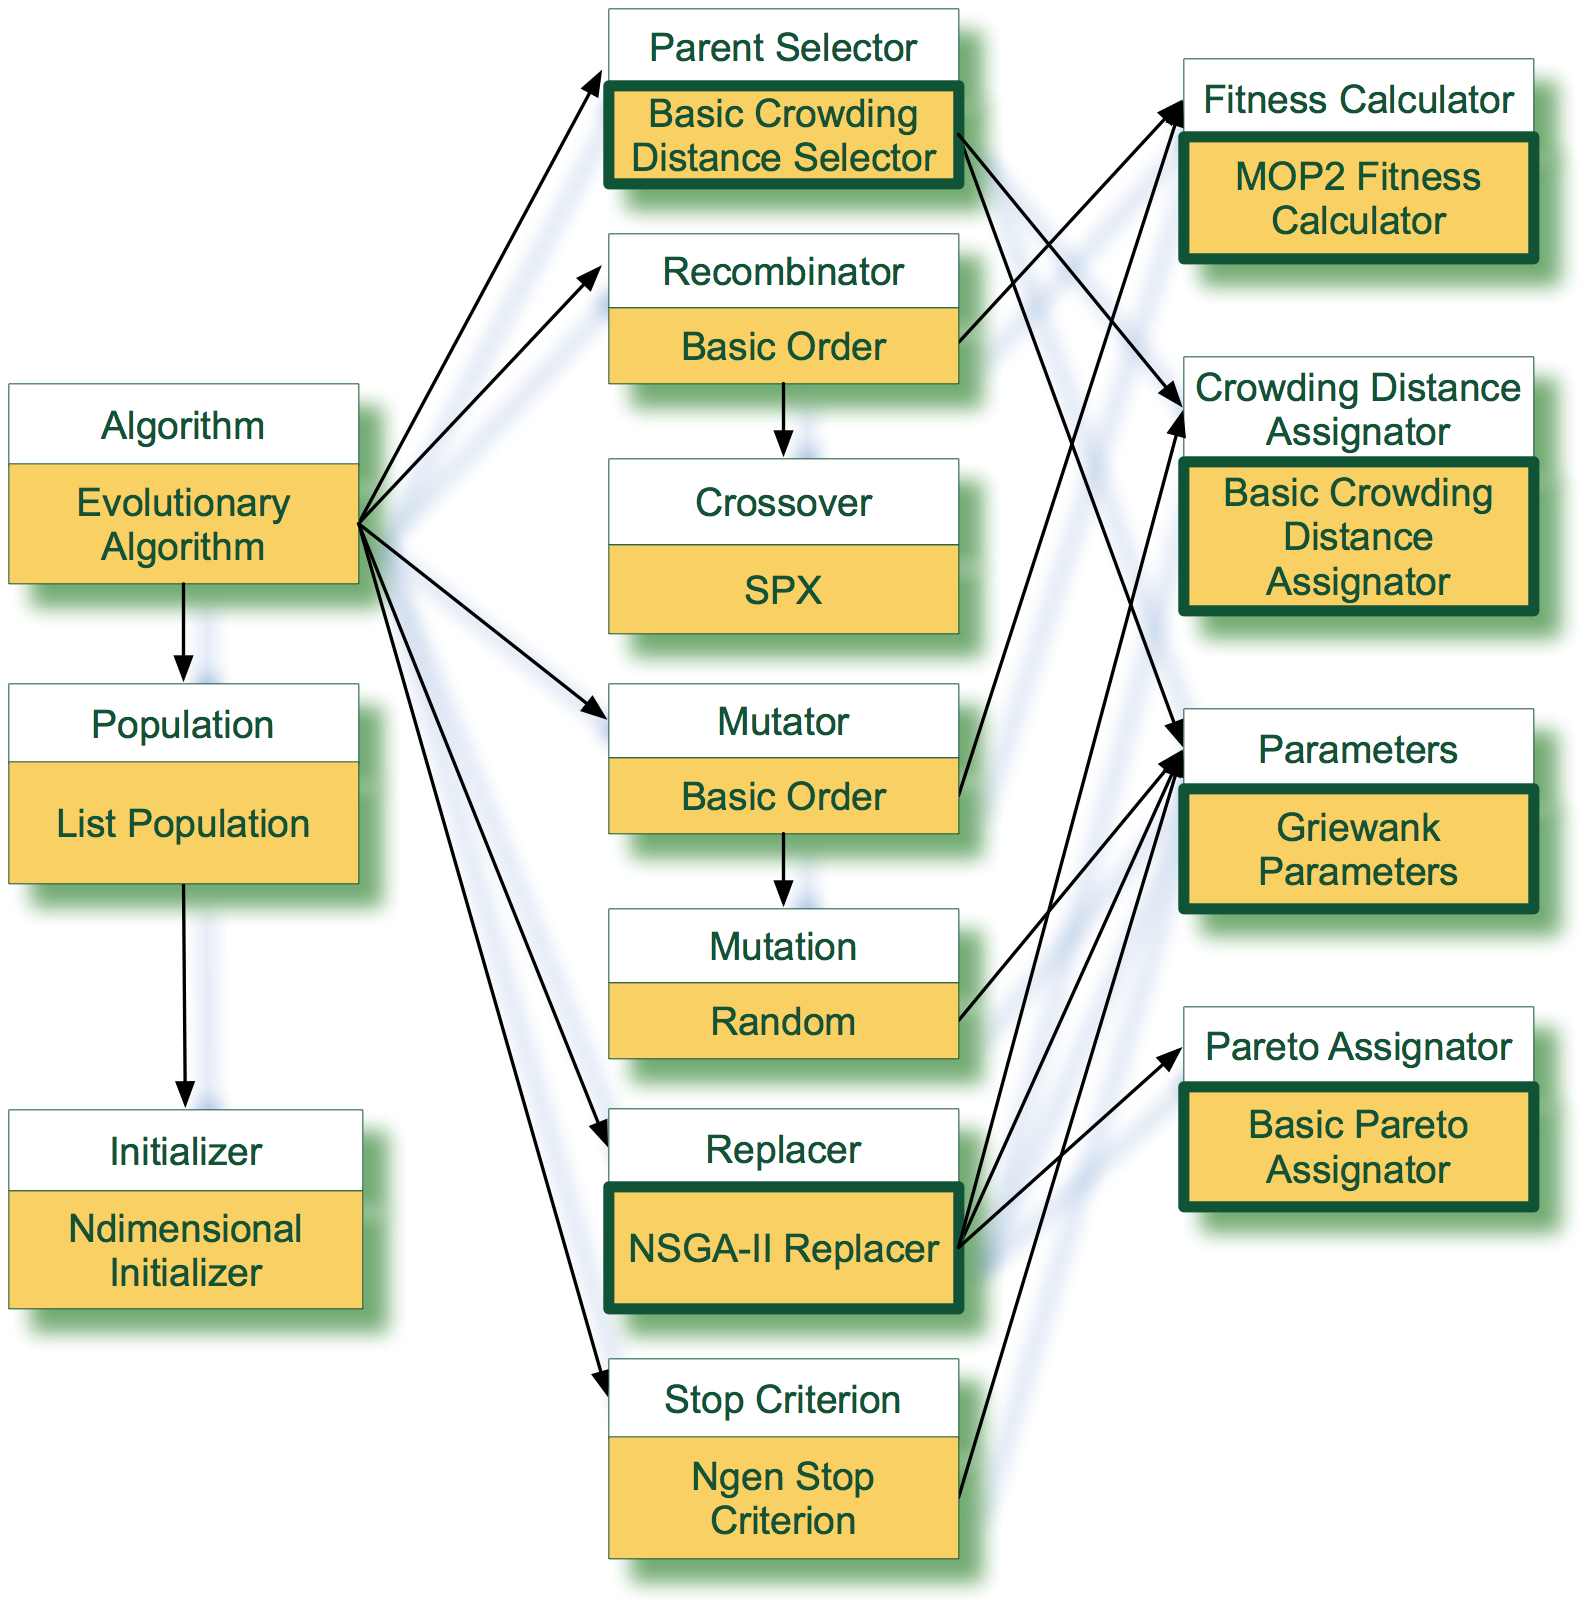
\includegraphics[width=10cm]{gfx/soaea/nsga2.jpg}
\caption{Modification of the basic GA adding new service implementations (orange blocks with thick lines).}
\label{fig:nsga2}
\end{SCfigure}



\subsection{Adding basic distribution}
\label{sec:distribution}

As every service must keep the same behaviour, independently of the machine that hosts it, distribution services for load balancing of a specific service can be easily created, for example, notifying the algorithm to use a distributed implementation for that service. As previously stated, the service {\em Fitness Calculator} receives a list of individuals to calculate their fitness, so, in this example, the new fitness implementation ({\em Basic Fitness Distributor}) binds with every fitness service available (in the same machine or in a network). The source code of this basic implementation simply distributes the list of individuals among the bound services and waits for their termination. Although more complex implementations probably will be more efficient, the objective of this section is to show how to distribute services, thus, this basic implementation is sufficient. Figure \ref{FITNESSDISTRIBUTOR} shows the modification from a sequential fitness calculator to a distributed one. Thanks to SOA, the number of distributed fitness calculators is not fixed: calculators can be added o removed in real time without stopping the system. As can be see in the figure, if one of the nodes is a cluster, it could also  implement another fitness distributor. This easy example can be adapted to more complex necessities depending on the infrastructure or the problem to be solved. More complex distribution services can be created, for example, taking into account communication latencies or computation capabilities of the nodes.




\begin{SCfigure}[20][htb]
\centering
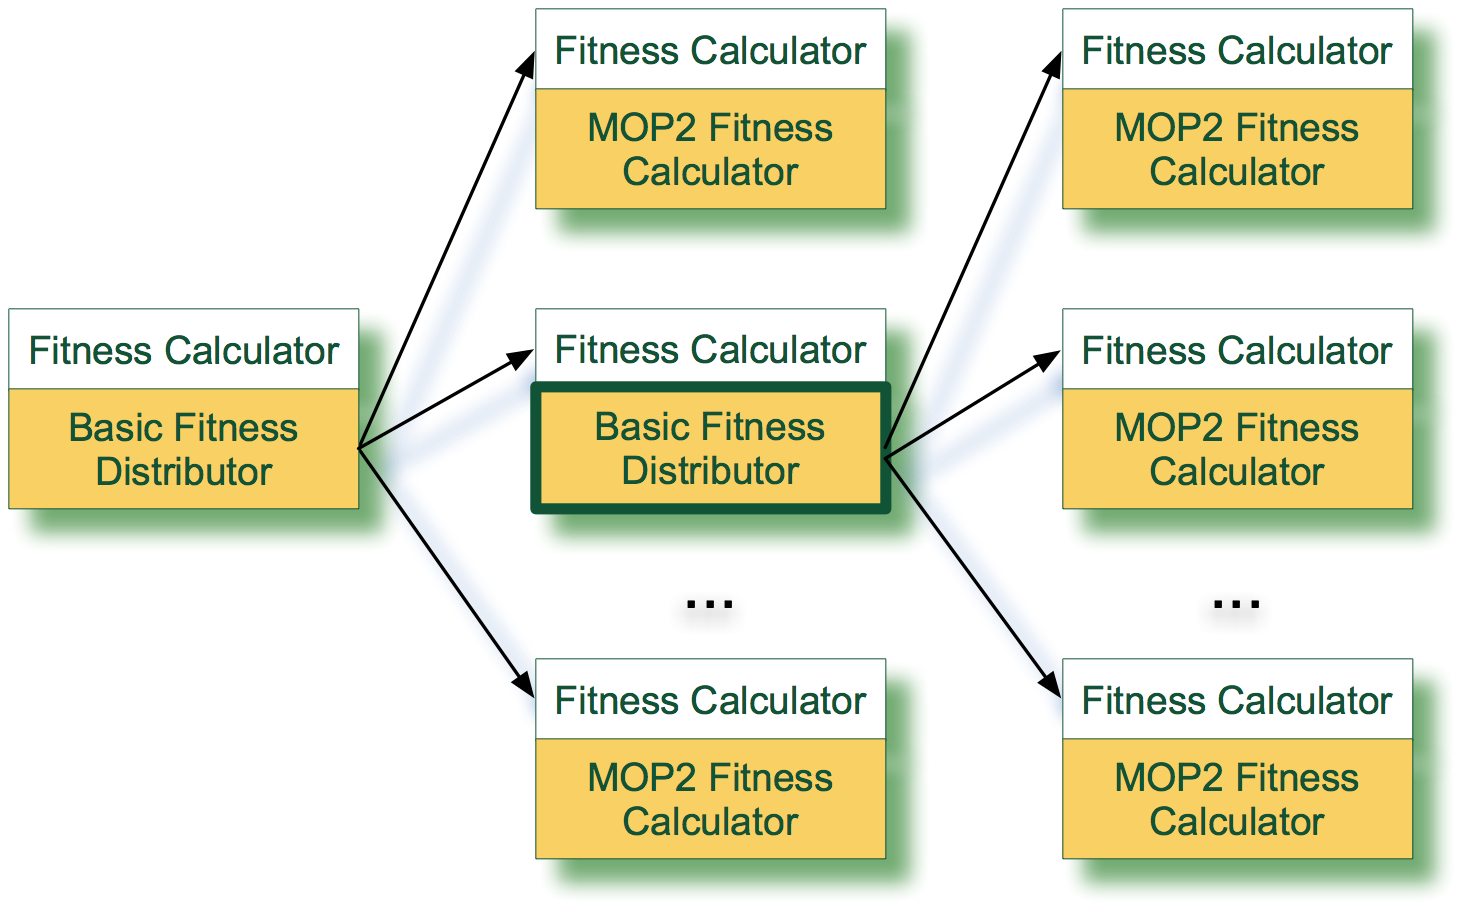
\includegraphics[width=10cm]{gfx/soaea/distributor.jpg}
\caption{Fitness distributor. The thick line implementation also re-distribute the individuals.}
\label{FITNESSDISTRIBUTOR}
\end{SCfigure}



One of the most extended model in parallel EAs is the island model. Using SOA-EA, the {\em Population} service implementation can be modified to become a distributed population. Each certain time, this population could exchange individuals with other populations modified by other algorithms. These populations should be added or deleted in execution time without affecting the algorithm execution. Figure \ref{POPULATION} shows this example, where a {\em Replacer} implementations maintains a list of references to other {\em Population} interfaces (which can be local or remote). Also other {\em Population} implementations exist ({\em List Population} is the usual list of individuals). If one of these population services drop, the others can continue working. The topology of these islands can also be managed from services (such as the {\em Basic Replacer} service, or another). The  modification and dynamism of the population structure is difficult to apply in existing frameworks without using SOA because it is necessary to create mechanisms to modify the population behaviour, the operators to modify it, the data structures, and also the code to manage all. With he usage of SOA, and due to the capability of accessing to a population via its service interface, it is not necessary to modify the source code to modify the population and its behaviour. Also, to avoid bottlenecks in distributed executions, asynchronous communication must be provided to avoid idle time. This kind of communication offers excellent performance when working with different nodes and operating systems, as demonstrated by \cite{Alba2002Heterogeneous}.



\begin{SCfigure}[20][htb]
\centering
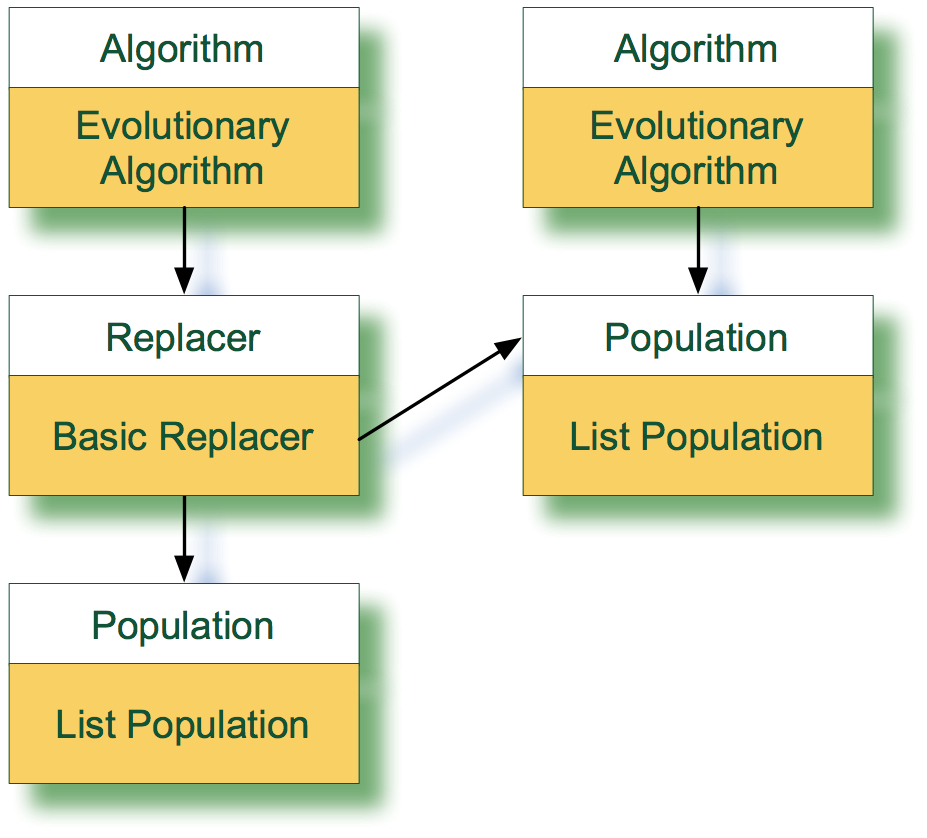
\includegraphics[width=10cm]{gfx/soaea/island.jpg}
\caption{Island model. From time to time, the Basic Replacer Implementation could send or receive individuals from another islands.}
\label{POPULATION}
\end{SCfigure}



\subsection{Self-adaptation in SOA-EA}
\label{sec:otherexamples}
There are several ways to create self-adaptable algorithms using SOA-EA. For example, creating a service that modifies the parameters in the {\em Parameters} service, or activating and de-activating operators in real time. An easier way is to create a service that manages all available services of the same kind. For example a {\em Mutator} service that binds all the available mutation implementations and use the most adequate one depending on some rules during the execution \cite{SelfadaptationSerpell2010}.  This idea can also be extended to create a service that implements several interfaces and selects the most adequate implementation for each interface respect to some criteria, as can be seen in Figure \ref{INTELLIGENTALGORITHM}, where thick lines represent the implementations used at the current moment (they vary as time passes).



\begin{SCfigure}[20][htb]
\centering
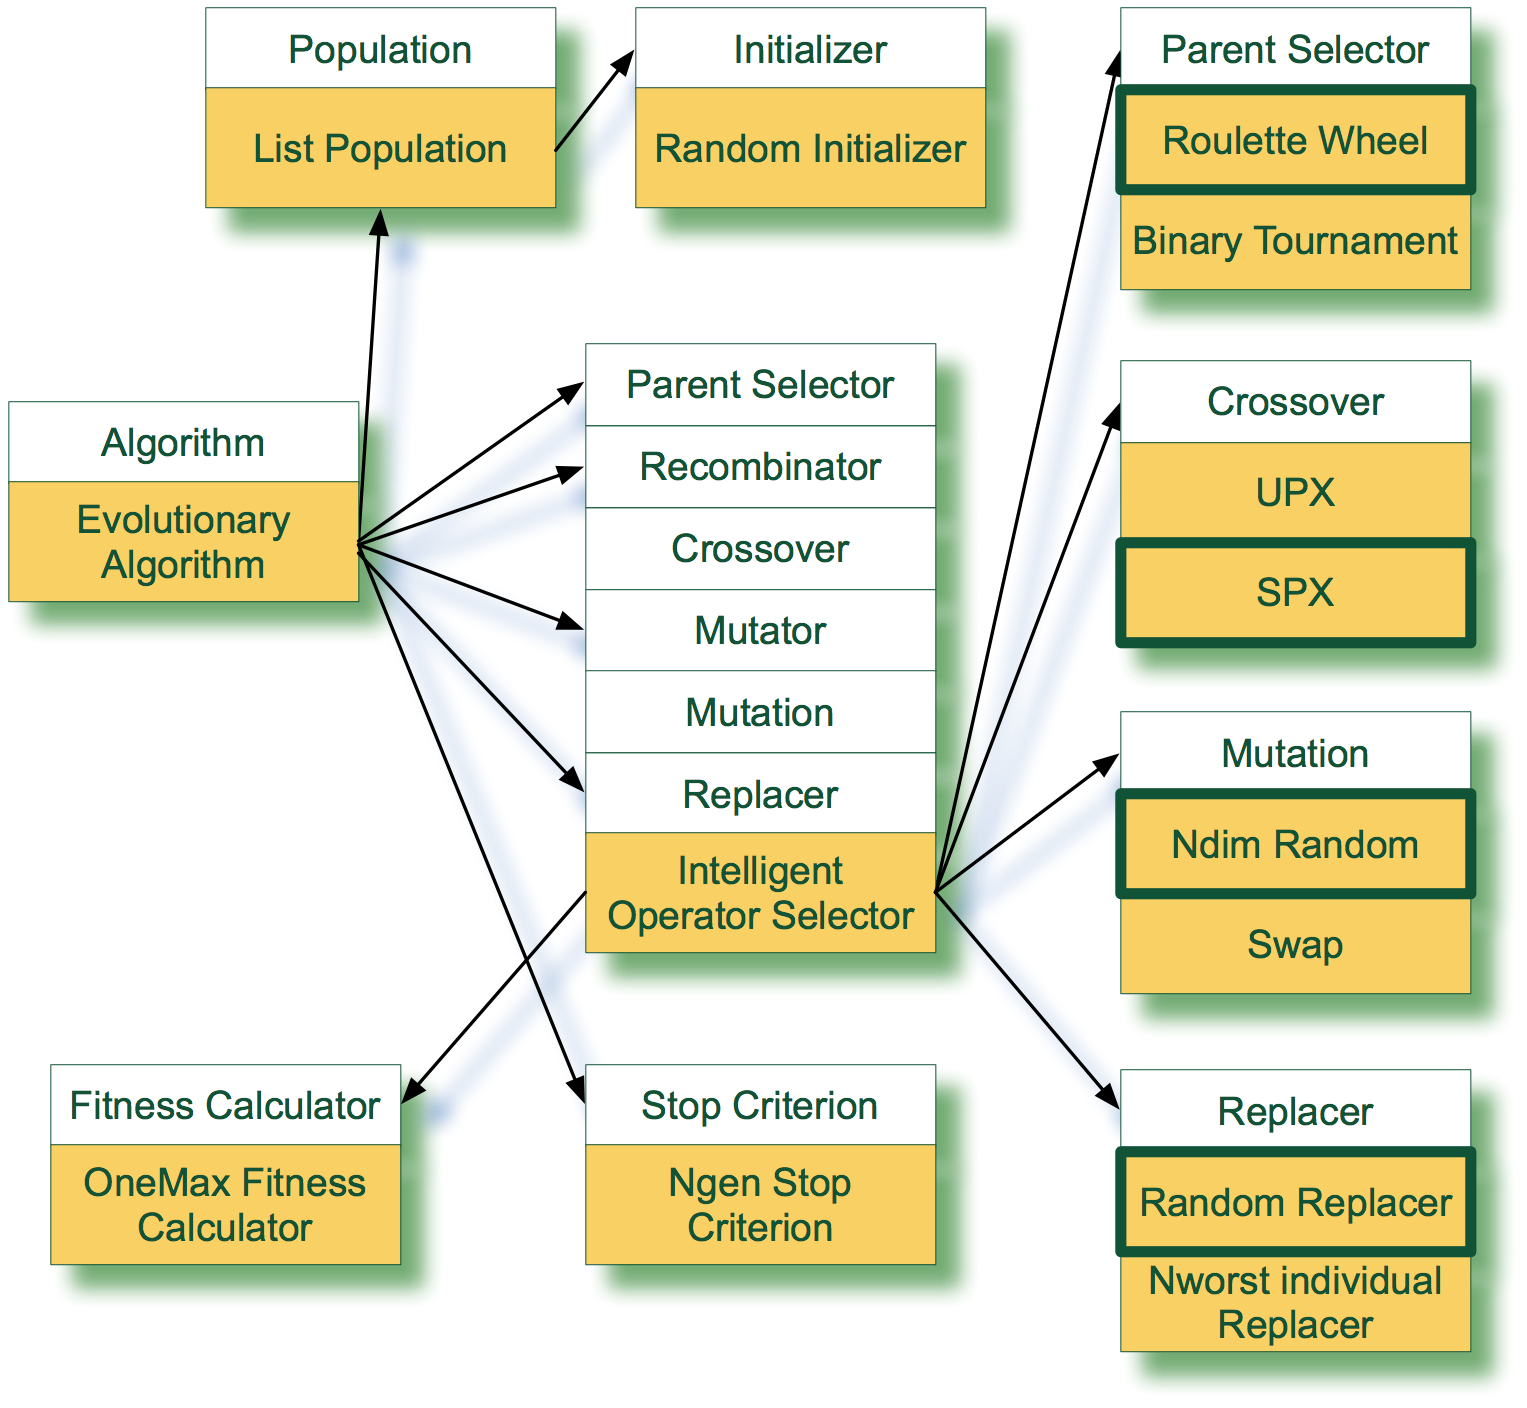
\includegraphics[width=10cm]{gfx/soaea/intelligent.jpg}
\caption{Self-adaptable Algorithm. The {\em Intelligent Operator Selector} selects which service implementation is used each time.}
\label{INTELLIGENTALGORITHM}
\end{SCfigure}


Finally, another important usage of EAs is its hybridization with other metaheuristics, to obtain more effective search algorithms \cite{HybridRodriguez2012},  increasing the performance of intensification and diversification mechanisms. With  traditional frameworks this task can be difficult, mainly because the source code for each metaheuristic must be modified. Nevertheless, using SOA a combination of loosely coupled services could be used.

\section{Conclusions}
In this chapter we have presented the requirements in the EA design: generic representation, generic fitness, generic operations, generic evolutionary model, parameter management and configurable output. On the other hand, the requirements in SOA have been also shown: genericity in the service interfaces, programming language independence, distribution transparency and flexibility. All these requirements have been taken into account to model the services that compose a generic EA, and several guidelines about the design of these services have been explained. We have presented the steps to create a service-oriented evolutionary algorithm that takes advantages of the SOA capabilities. It has been explained how to modify the services to change from a model to another, adding transparent distribution and load-balancing or dynamic adaptation of the parameters.

In a later chapter, we will use a specific SOA technology (OSGi) to implement the examples shown in previous sections, and how to accomplish the requirements in the development of EAs and SOA, taking advantage of the capabilities of SOA.


}{\myChapter{A methodology for developing services for EAs}\label{chap:soaea}}
%\ifthenelse{\equal{\value{IncluyeCapitulo}}{8}}{\myChapter{Recomendaciones para el Dise�o de Cuestionarios de Calidad de Contornos} \label{chap:recCuestCalidadBordes} \minitoc\mtcskip
\vfill
\lettrine{M}{uchos} autores indican que no es posible proporcionar un �nico e infalible conjunto de reglas, protocolos o metodolog�as para la correcta construcci�n o dise�o de cuestionarios, que eliminen completamente todo tipo de sesgo. En general, lo que se proponen son recomendaciones en el dise�o de las preguntas y de los cuestionarios para minimizar dicho sesgo. Como se ha indicado en cap�tulos anteriores, existen algunas recomendaciones de dise�o en el plano ling\"{u}�stico para la realizaci�n de cuestionarios. Sin embargo, no existen recomendaciones para cuestionarios en los que se incluyan elementos multimedia.\\
\noindent Se inicia identificando el nuevo \emph{sesgo por finalidad} y describiendo algunas recomendaciones para mitigar su efecto. Se contin�a aportando algunas recomendaciones de dise�o para cuestionarios que involucren preguntas con elementos visuales, y en particular, para la evaluaci�n subjetiva de la calidad de algoritmos de extracci�n de contornos. Para finalizar este cap�tulo, se presenta una herramienta Web para la creaci�n y difusi�n de los cuestionarios, que permite contestarlos \mbox{on--line}, y que facilita al investigador la recolecci�n de las respuestas.
\clearpage
\section{Sesgo por finalidad}\label{sec:sesgo-finalidad}
\lettrine{E}{l} \emph{Sesgo por finalidad} se produce cuando los encuestados conocen los objetivos asociados a la pregunta que est�n respondiendo y, por tanto, las respuestas pueden estar influenciadas por ello. En algunos casos, el efecto producido por el \emph{Sesgo de deseabilidad social} es similar, puesto que los encuestados no contestan seg�n sus opiniones propias, sino las que los encuestados creen que son las que mayor aprobaci�n social tendr�n. En cierto modo, los encuestados escogen las opciones influenciados por lo que ellos creen que el entrevistador desea que ellos contesten. En estos casos, las recomendaciones de dise�o indican que las preguntas que puedan sufrir de alg�n tipo de \emph{Sesgo de deseabilidad social} deben hacerse en un tono neutral y mediante preguntas indirectas, de tal forma que sea m�s complicado percibir la intencionalidad (los objetivos subyacentes asociados) de dichas preguntas.\\
Las encuestas que tratan de estimar la calidad de alg�n proceso suelen depender de la finalidad con la que se aplique dicho proceso. Es decir, que un mismo proceso puede proporcionar un resultado muy positivo para una aplicaci�n determinada, y muy negativo para otras. Por ejemplo, un medicamento puede ser muy eficaz para tratar una enfermedad y, a la vez, estar contraindicado para otras. Este sesgo puede aparecer en diferentes escenarios: cuando el entrevistado conoce (directamente informado por el entrevistado o porque ha sido capaz de deducirlo) la finalidad del proceso sobre el que se le est� encuestando, o cuando cree conocer dicha finalidad y realmente se confunde a s�� mismo, proporcionando respuestas totalmente err�neas. Normalmente, suele estar causado por una incorrecta redacci�n de las preguntas por parte del entrevistador, no dejando claramente especificada la finalidad de cada pregunta.\\
\noindent En el caso de las encuestas de calidad, en muchos casos hay que guiar al encuestado sobre qu� debe observar o analizar, proporcion�ndole en estos casos el objetivo de la pregunta. Por ejemplo, si en una cata ciega de un nuevo producto se desea que los usuarios den su opini�n sobre un determinado aspecto del mismo, habr��a que indicarles que se deben centrar en un aspecto en particular, ya que no se desea conocer otros aspectos de ese producto. Concretando el ejemplo, si el producto fuese una bebida, se podr��a preguntar en exclusiva sobre el dulzor, la acidez, la textura, etc. Sin embargo, puede que ese aspecto en particular no sea el que m�s llame la atenci�n a los encuestados, o incluso, que si no se le hubiese preguntado espec��ficamente por �l, habr��a pasado desapercibido. En estos casos, aunque los encuestados proporcionen las respuestas basadas en su propia opini�n, �stas est�n influidas por el \emph{Sesgo por finalidad}.\\
\noindent En la mayor��a de los casos en los que aparece este tipo de sesgo, �ste se introduce debido a que el dise�ador de la encuesta necesita indicar a los encuestados el objetivo que se est� buscando en cada pregunta, para centrar la atenci�n de los encuestados en dicho aspecto, descartando otros elementos presentes en dicha pregunta. Se plantean dos posibilidades:
\begin{aenumerate}
\item No informar a los encuestados de la finalidad de cada pregunta, permitiendo que las respuestas de los encuestados no se ajusten a los objetivos de cada pregunta.
\item Informar a los encuestados de la finalidad en cada pregunta, asumiendo que se est� introduciendo este tipo de sesgo en todas las preguntas.
\end{aenumerate}

\noindent Con la primera posibilidad, se elimina el \emph{Sesgo por finalidad}, ya que se est� omitiendo la informaci�n de la finalidad de las preguntas, por lo que no se influye a los encuestados. Sin embargo, no hay garant��a de que los encuestados proporcionen respuestas que sirvan para contestar a los objetivos asociados a cada pregunta.\\
\noindent Por el contrario, con la segunda posibilidad se introduce expl��citamente este sesgo en todas las preguntas. De esta manera se reduce la libertad de los encuestados en las posibles respuestas, pero se intenta garantizar un nivel de conocimiento base que permita a los encuestados proporcionar respuestas que sean interesantes para el evaluador en el contexto para el que ha desarrollado la pregunta. Esta segunda opci�n es admisible si se informa a todos los encuestados de los objetivos de cada una de las preguntas del cuestionario. No es conveniente mezclar en un mismo cuestionario preguntas en las que se indique el objetivo de las mismas con otras preguntas en las que esto no se indique, ya que, al estar m�s guiadas unas respuestas que otras, los resultados no son comparables.

\section{Recomendaciones generales sobre las preguntas}
\lettrine{C}{on} los cuestionarios indicados en esta Tesis se intenta evaluar de manera subjetiva qu� algoritmo de procesamiento de im�genes se comporta de mejor manera ante un determinado entorno de funcionamiento (que viene determinado por los \textsc{Dominios} del cuestionario). A continuaci�n, se muestra la estructura que se recomienda que tenga un cuestionario.
\subsection{Estructura de las preguntas}
Se considera que un cuestionario est� compuesto por una o varias preguntas; y cada pregunta est� compuesta por:

\begin{aenumerate}
\item Un texto de introducci�n y de pregunta.
\item Una imagen original [Optativa].
\item Una o varias \emph{im�genes respuesta}, cada una con su zona de respuesta asociada.
\end{aenumerate}

\noindent Se ha considerado que lo m�s eficiente para este tipo de cuestionarios es no mezclar preguntas que contengan elementos visuales con preguntas de tipo exclusivamente ling\"{u}�stico. Si se mezclan ambos tipos de preguntas, la evaluaci�n se complica mucho para el entrevistador. Como se ver� m�s adelante, cada pregunta tiene ponderada su contribuci�n al resultado final, y conseguir dicho factor de ponderaci�n en preguntas exclus�vamente ling\"{u}�sticas es muy complejo. Adem�s, se han realizado diversas pruebas con cuestionarios experimentales (pruebas de pilotaje inicial), que han mostrado que los entrevistados mostraban mayores dificultades al responder cuestionarios con mezcla de ambos tipos de preguntas (ling\"{u}�sticas y visuales) que los cuestionarios con preguntas de un �nico tipo. Los entrevistados argumentaron que les ``costaba'' ir cambiando de formato de pregunta cuando ya se hab�an acostumbrado a responder preguntas de un determinado tipo.
\subsection{Im�genes respuesta}
Las \emph{im�genes respuesta} son las distintas im�genes de respuesta asociadas a cada pregunta, donde se busca que el entrevistado responda a la cuesti�n planteada en el ``texto de introducci�n y de pregunta''. En dicho texto se solicita al entrevistado que realice alguna tarea de visi�n (\textsc{detecci�n}, \textsc{orientaci�n}, \textsc{reconocimiento} o \textsc{identificaci�n}) utilizando en cada caso la \emph{imagen respuesta} correspondiente. Cada una de ellas tendr� asociado un �nico algoritmo de procesamiento de im�genes.
\subsection{Ponderaci�n de preguntas}
No todas las preguntas tienen el mismo valor para obtener el resultado final, puesto que hay algunas preguntas que pueden ser discriminatorias, mientras que otras pueden matizar el grado de especializaci�n. T�mese como ejemplo, una pregunta en la que se solicite que se indiquen aquellas \emph{im�genes respuesta} en las que se pueda detectar un determinado objeto, sin importar si se detecta mejor o peor. Todas aquellas \emph{im�genes respuesta} en las que no sea apreciable dicho objeto obtendr�n baja puntuaci�n, y por lo tanto, los algoritmos de procesamiento de im�genes asociados a esas \emph{im�genes respuesta} conseguir�n pocos puntos. Pero adem�s, desde un punto de vista global, esa pregunta es altamente discriminatoria, es decir, que para la puntuaci�n global de los algoritmos de procesamiento de im�genes, existe una gran diferencia en el grado de colaboraci�n en la puntuaci�n final de los casos en los que los entrevistados pueden detectar el objeto frente a los casos en los que no pueden detectarlo. Por tanto, cada pregunta colaborar� con el resultado final con un cierto grado, especificado utilizando valores de ponderaci�n, que podr�n variar seg�n las distintas clases de respuestas posibles.\\
\noindent A pesar de que este comportamiento es altamente deseable, una ponderaci�n de todas las preguntas de un cuestionario que sea satisfactoria y que no presente ni \emph{sesgo} ni favorezca \apriori ning�n m�todo es muy dif�cil de conseguir. Para poder simplificar la tarea del dise�o de la encuesta, en esta Tesis Doctoral no se aplicar�n distintas ponderaciones, sino que todas las preguntas colaborar�n en la misma proporci�n en el c�lculo del resultado final.
\clearpage
\section{Tipos de preguntas con elementos visuales}
\lettrine{L}{os} posibles tipos de preguntas que se consideran en los cuestionarios de calidad de bordes en im�genes son los de:

\begin{aenumerate}
\item Preguntas con respuestas de \textsc{selecci�n} (o \textsc{dicot�micas}).
\begin{aenumerate}
    \item \textsc{Con repetici�n} (Varias \emph{im�genes respuesta} v�lidas).
    \item \textsc{Sin repetici�n} (S�lo una \emph{imagen respuesta} v�lida).
\end{aenumerate}
\item Preguntas con respuestas de \textsc{puntuaci�n}.
\begin{aenumerate}
    \item \textsc{Con repetici�n} (Varias \emph{im�genes respuesta} pueden tener la misma puntuaci�n).
    \item \textsc{Sin repetici�n} (Cada \emph{imagen respuesta} tiene una puntuaci�n, y dicha puntuaci�n no ha sido asignada a ninguna otra imagen respuesta).
\end{aenumerate}
\item Preguntas con respuestas de \textsc{ordenamiento}.
\begin{aenumerate}
    \item \textsc{Con repetici�n} (Varias \emph{im�genes respuesta} pueden tener el mismo valor de asignaci�n).
    \item \textsc{Sin repetici�n} (Cada \emph{imagen respuesta} tiene un valor �nico de ordenamiento).
\end{aenumerate}
\item Preguntas con respuesta de \textsc{mapeado espacial y temporal} (o \textsc{Mapping}).
\end{aenumerate}

\subsection{Preguntas de \textsc{selecci�n} o \textsc{dicot�micas}}
Mediante este tipo de preguntas se busca encontrar en cu�les de las \emph{im�genes respuesta} el entrevistado puede realizar la tarea de visi�n encomendada en el texto de la pregunta. Para desambiguar cualquier posible duda que pudiera tener el entrevistado, el entrevistador debe especificar con la mayor claridad posible en el texto de la pregunta en qu� casos puede el entrevistado seleccionar la \emph{imagen respuesta} en funci�n de la realizaci�n de la tarea de visi�n (por ejemplo, si puede realizar perfectamente la tarea de visi�n encargada sin ninguna dificultad, o en otro caso distinto, si puede realizar al menos m�nimamente la tarea de visi�n aunque con un cierto grado de dificultad, etc.).
\paragraph{Sin repetici�n} \noindent Utilizando el mecanismo \textsc{sin repetici�n}, el entrevistador consigue un beneficio directo: obliga al entrevistado a escoger s�lo una de las \emph{im�genes respuesta}, a pesar de que quiz�s �ste pudiera realizar la tarea de visi�n encomendada en varias de ellas. El principal handicap que comentan los entrevistados sobre esta opci�n es que es poco natural, debido a que les fuerza a escoger, a�n cuando no lo desean. Un beneficio adicional que se consigue con este mecanismo es que �ste se puede considerar un selector elitista, es decir, que permite discriminar con mayor claridad cu�l es considerado el ``mejor'' algoritmo (asociado a una \emph{imagen resultado}), ya que �ste obtiene toda la puntuaci�n, mientras que el resto no obtiene ning�n punto.
\paragraph{Con repetici�n} \noindent Por el contrario, el mecanismo \textsc{con repetici�n} permite un mayor grado de libertad al entrevistado, ya que �ste no tiene que escoger s�lo una \emph{imagen respuesta}. Esta opci�n es mucho m�s natural, ya que si no existen excesivas diferencias entre los resultados de los distintos algoritmos que se est�n evaluando, es mucho m�s realista para un entrevistado afirmar que es capaz de realizar una determinada tarea de visi�n con varias \emph{im�genes respuesta} similares. Sin embargo, al contrario que en el mecanismo anterior, �ste permite una menor discriminaci�n al obtener igual puntuaci�n varios de los algoritmos (pudiendo incluso seleccionar todas las \emph{im�genes respuesta}).
\subsection{Preguntas de \textsc{puntuaci�n}}
Gracias a estas preguntas, el entrevistador puede conocer el grado de calidad intr�nseca percibida por los entrevistados asociada a la utilizaci�n de cada \emph{imagen respuesta} para realizar una tarea de visi�n (especificada en el ``texto de la pregunta'').\\
\noindent La utilizaci�n de varias im�genes permite a los entrevistados compararlas, por lo que en esos casos, la puntuaci�n que se asigne se puede considerar m�s como el grado de comparaci�n entre las im�genes que como la evaluaci�n individual de cada una. Al permitirse la comparaci�n entre las im�genes, los entrevistados incorporan m�s informaci�n al puntuar cada imagen que la incluida en la propia imagen, ya que pueden mirar el resto. En muchos casos, la puntuaci�n de cada \emph{imagen respuesta} se realiza valorando cada imagen con una imagen ``virtual'' que cada entrevistado se construye de manera heur�stica en su propia mente utilizando informaci�n visual de cada \emph{imagen respuesta}. Por tanto, en las preguntas que se utilicen m�s de una \emph{imagen respuesta} el entrevistador debe admitir la existencia de un cierto grado de \emph{sesgo por finalidad}, que debe ser minimizado mediante la inclusi�n de otras preguntas en las que no se muestren m�ltiples \emph{im�genes respuesta}.
\paragraph{Sin repetici�n} \noindent Utilizando el mecanismo \textsc{sin repetici�n}, el entrevistador fuerza a los entrevistados a asignar diferente puntuaci�n a todas las \emph{im�genes respuesta}. Si la puntuaci�n es un valor real, esta opci�n no tiene utilidad pr�ctica, por la facilidad que existe para modificar la puntuaci�n decimal. Por el contrario, si es un valor entero, se provoca una cierta distanciaci�n entre las \emph{im�genes respuesta}, lo que permite una mayor discriminaci�n en las respuestas. Sin embargo, esa diferenciaci�n puede ser totalmente ficticia, en el sentido que los entrevistados pueden encontrar una diferencia entre las \emph{im�genes respuesta} menor que la que le obliga la asignaci�n sin repetici�n y con valores enteros.
\paragraph{Con repetici�n} \noindent Por el contrario, el mecanismo \textsc{con repetici�n} permite una mayor flexibilidad a los entrevistados para asignar puntuaci�n. Al permitir la repetici�n, a veces, los entrevistados tienden a agrupar puntuaciones, es decir, asignan la misma puntuaci�n a todas las \emph{im�genes respuesta} que tienen una calidad elevada, sin precisar si en alguna de ellas la calidad es mayor o menor.
\subsection{Preguntas de \textsc{ordenamiento}}
Gracias a estas preguntas, el entrevistador puede conocer el orden de calidad percibida comparada por los entrevistados asociada a la utilizaci�n de cada \emph{imagen respuesta} para realizar una tarea de visi�n (especificada en el ``texto de la pregunta''). Como su propio nombre indica, el entrevistado ``ordena'' de mejor a peor las im�genes, asignando un valor num�rico a cada \emph{imagen respuesta} que permite organizarlas comparativamente. Con este tipo de preguntas, el entrevistador no tiene garant�a de que el entrevistado haya sido capaz de realizar la tarea de visi�n solicitada: s�lo se solicita que ordene de mejor a peor las \emph{im�genes respuesta}, cuando quiz�s el entrevistado no haya sido capaz de realizar la tarea encomendada, aunque de manera subjetiva es capaz de indicar con cu�l se siente m�s c�modo.\\
\noindent Se puede afirmar que este tipo de preguntas es menos exigente para el entrevistado que las de \textsc{puntuaci�n}, ya que al no tener que puntuar, no tiene que comparar mentalmente cada \emph{imagen respuesta} con la \emph{imagen respuesta} ``perfecta'' (que, previamente, el entrevistado se habr� formado en su mente); le basta con ordenar las existentes. Debido a la simplificaci�n en la evaluaci�n, este tipo de preguntas no proporcionan resultados excesivamente discriminantes. Un cuestionario realizado exclusivamente con este tipo de preguntas s�lo proporcionar�a \emph{tendencias} generales y para obtener resultados m�s concretos, estas preguntas se deben formular a�adidas a otras de otros tipos.
\paragraph{Sin repetici�n} \noindent Utilizando el mecanismo \textsc{sin repetici�n}, el entrevistador obliga que el entrevistado no pueda indicar que dos o m�s \emph{im�genes respuesta} son iguales o tienen la misma calidad para realizar la ``tarea de visi�n''. Este aspecto incrementa ligeramente la discriminaci�n, pero los entrevistados suelen mostrarse molestos por tener que escoger entre uno en particular y se pueden producir peque�os \emph{sesgos} con respecto a la posici�n de las \emph{im�genes respuesta} entre las que tiene que escoger (existiendo una leve preferencia hacia las que se encuentran a la izquierda, probablemente por ser la tendencia natural de la escritura occidental, de izquierda a derecha).
\paragraph{Con repetici�n} \noindent Por el contrario, el mecanismo \textsc{con repetici�n} permite mayor libertad a los entrevistados para clasificar las \emph{im�genes respuesta}, a costa de que dichas respuestas suelen tener menor discriminaci�n que el tipo anterior.

\subsection{Preguntas de \textsc{mapeado espacial y temporal}}
Mediante este tipo de preguntas, el entrevistador puede comprobar la precisi�n espacial y el tiempo que tardan los entrevistados en realizar las ``tareas de visi�n'' encomendadas. Estas preguntas, tambi�n llamadas de \textsc{Mapping}, s�lo admiten una \emph{imagen respuesta}, sobre la cual el entrevistado debe marcar en la posici�n en la que el propio entrevistado estima que se encuentra la caracter�stica solicitada en el texto de la pregunta. El entrevistador deber� tener se�alado en una copia propia de la \emph{imagen respuesta}, que no mostrar�a en ning�n caso al entrevistado, la posici�n exacta de la caracter�stica buscada, a lo que se ha dado en denominar \emph{punto} (o \emph{zona}) \emph{objetivo}. El encuestador podr� se�alar zonas de precisi�n, es decir, zonas alrededor del \emph{punto objetivo} que podr�n tener distinta ponderaci�n. Mediante esta opci�n se controla la precisi�n espacial. En el caso de que la caracter�stica buscada sea marcable de manera puntual, bastar� con que el entrevistado se�ale dicho punto (por ejemplo, con el puntero del rat�n). Si la caracter�stica fuese una zona, el entrevistado tendr�a que marcar varios puntos que delimitasen dicha zona, para lo cual el sistema (si fuese por computador) podr�a facilitar el trabajo del entrevistado permitiendo el manejo autom�tico de estructuras poligonales. Esta opci�n, sin embargo, presenta un inconveniente que es el manejo de los errores (�reas que se encuentren fuera de la zona marcada por el entrevistador como \emph{zona objetivo}).\\
\noindent En muchas aplicaciones, la precisi�n espacial es importante, pero dentro de unos l�mites temporales. Es decir, existen situaciones en las que el entrevistado deber�a responder antes de un cierto tiempo, a partir del cual, la consideraci�n de la respuesta podr�a estar muy degradada o incluso puede no ser aceptable en absoluto (a pesar de que la misma fuese perfecta en cuanto a la precisi�n espacial). Para controlar esta opci�n el sistema debe controlar el tiempo de respuesta de los entrevistados ante la presentaci�n del est�mulo (la \emph{imagen respuesta}). En estos casos, se debe mostrar el texto de la pregunta a los entrevistados manteniendo la \emph{imagen respuesta} oculta hasta que �ste indique que est� preparado y se empiece a contar el tiempo. El encuestador debe tener una funci�n matem�tica que permita ponderar el tiempo de respuesta del entrevistado.\\
Utilizando este tipo de preguntas, el encuestador puede cruzar datos con otras preguntas y comprobar si realmente los entrevistados est�n realizando la ``tarea de visi�n'' encomendada. Esto permite controlar incorrecciones por parte de los encuestados. Por ejemplo, en otros tipos de preguntas, los entrevistados podr�an afirmar que son capaces de detectar un cierto objeto en una determinada \emph{imagen respuesta}, y sin embargo, al proponerles que se�alen donde se encuentra dicho objeto mediante una pregunta de \textsc{Mapping}, el entrevistado se�ala en otra zona distinta o no con demasiada precisi�n, o tarda mucho tiempo en determinar la posici�n exacta. Esto significar�a que la respuesta que dieron a la otra pregunta no era demasiado veraz, y por tanto, habr�a que tener mucha cautela al incluir dichas respuestas en el c�lculo final.\\
\noindent El principal inconveniente que presenta este tipo de preguntas es que s�lo se pueden evaluar una \emph{imagen respuesta} cada vez. Tambi�n hay que indicar que son un poco m�s dif�ciles y algo m�s tediosas de contestar que el resto.\\
\noindent Para finalizar, se ha de indicar que este tipo de preguntas se presenta como una aportaci�n especial de esta Tesis, y se ha dise�ado haciendo uso espec�fico del soporte inform�tico, aunque con algunas peque�as adaptaciones podr�a utilizarse en encuestas ``en papel''.
\clearpage
\section{Recomendaciones sobre la estructura general del cuestionario}
A continuaci�n, se analizan algunos aspectos que tienen una influencia en el dise�o del cuestionario y se propondr�n una serie de recomendaciones sobre la estructura del cuestionario. La mayor�a de estas recomendaciones intentan reducir el \emph{sesgo} que el uso de contenidos visuales puede introducir en el cuestionario en general y en cada pregunta en particular.\\
\subsection{Reutilizaci�n de im�genes}
Uno de los primeros aspectos que se consideran cuando se dise�a un cuestionario con contenidos visuales, es la reutilizaci�n de esos mismos contenidos visuales. Esta reutilizaci�n se presenta en dos vertientes, utilizar exactamente las mismas \emph{im�genes respuesta}, obtenidas utilizando el mismo m�todo de procesamiento de im�genes con los mismos par�metros, o bien, utilizar la misma imagen original y obtener diferentes \emph{im�genes respuesta} (ya sea variando el m�todo de procesamiento de im�genes, modificando los par�metros aplicados o ambos casos) que son representaciones visuales de la misma imagen original.\\
\noindent Se ha podido observar que los entrevistados \emph{recuerdan} las caracter�sticas de las im�genes reutilizadas, produci�ndose un \emph{sesgo} en la respuesta de los mismos. Para comprobar este comportamiento se realiz� un experimento en los que los entrevistados ten�an que puntuar la calidad de los mapas de bordes de ciertas \emph{im�genes respuesta}. El cuestionario estaba compuesto por 5 preguntas. En cada pregunta se aplicaba un mismo m�todo de procesamiento de bordes sobre la misma imagen original, variando los par�metros de dicho m�todo, obteniendo las \emph{im�genes respuesta} que se comparaban en cada pregunta.\graffito{La reutilizaci�n de im�genes fomenta el \emph{recuerdo} de las mismas.} Sin conocimiento de los entrevistados, la primera pregunta y la �ltima pregunta del cuestionario eran id�nticas y mostraban exactamente las mismas \emph{im�genes respuesta}, incluyendo el mismo orden de presentaci�n de las mismas. Se pudo observar que todos los entrevistados respondieron de manera an�loga en la primera y en la �ltima pregunta, sin embargo, en general tardaron mucho menos en contestar la �ltima pregunta que la primera, a pesar de que eran iguales. Tras finalizar la encuesta, se les pregunt� porqu� hab�an tardado menos en responder a la �ltima pregunta que a la primera y todos ellos respondieron que ``\emph{ya conoc�an las im�genes}''.\\
\noindent En el caso de uso de preguntas con respuestas de \textsc{mapeado espacial y temporal}, d�nde tanto la precisi�n de la respuesta como el tiempo de respuesta influyen en la calidad de la misma, la reutilizaci�n de im�genes es un elemento cr�tico. Si utilizando este tipo de preguntas se pretende evaluar la calidad de varios m�todos o del mismo m�todo con diferentes par�metros, es imprescindible utilizar la misma imagen original. Para estudiar la influencia de la reutilizaci�n de la misma imagen original en preguntas con respuestas de \textsc{mapeado espacial y temporal}, se realiz� un peque�o estudio mediante un cuestionario compuesto �ntegramente por preguntas de \textsc{Mapping} en las que se utilizaban \emph{im�genes respuesta} que part�an de la misma imagen orignal con diferentes m�todos de procesamiento de im�genes. En todas las preguntas de \textsc{Mapping} se solicitaba a los encuestados que marcasen d�nde consideraban que se encontraba un cierto objeto. Se pudo observar que la precisi�n espacial de los entrevistados mejoraba conforme iban respondiendo a m�s preguntas que utilizaban la misma imagen original, casi independientemente del grado de calidad de la \emph{imagen respuesta}. Es decir, al ir respondiendo preguntas, las respuestas iban aumentando la precisi�n espacial, siempre que el m�todo de extracci�n de bordes obtuviese algunos contornos del objeto que se buscaba, sin necesidad de que el contorno del objeto se hubiese obtenido completamente. Se pudo observar un comportamiento interesante y es que en cuanto los entrevistados contestaban a alguna pregunta en la que el contorno del objeto estuviese completo, en todas las preguntas posteriores la precisi�n espacial de la respuesta era muy elevada. Se puede decir, que en cuanto consegu�an encontrar el objeto por primera vez, ya lo encontraban siempre.\\
\noindent M�s evidente fue el an�lisis del tiempo de respuesta,\graffito{El tiempo de b�squeda en preguntas de \textsc{Mapping} con im�genes repetidas se va reduciendo conforme se contestan m�s preguntas con la misma imagen original.} en el que se pudo observar como dicho tiempo de respuesta se reduc�a al responder m�s preguntas, llegando a ser casi constante en las �ltimas, pr�cticamente sin influencia de la calidad de la \emph{imagen respuesta} que se mostrase. Se puede afirmar que los entrevistados recordaban la zona de la imagen d�nde se encontraba el objeto y no ten�an que volver a buscarlo por toda la imagen. Tambi�n, se puede indicar que el proceso de b�squeda y detecci�n se realizaba cada vez de manera m�s autom�tica por parte de los encuestados tras responder a m�s preguntas que se basan la misma imagen original.\\
\noindent Por tanto, si se reutilizan im�genes en preguntas con respuestas de \textsc{mapeado espacial y temporal}, ?`cu�ntas preguntas con otras im�genes diferentes hay introducir entre medio para que los entrevistados \emph{olviden} la imagen? Para responder a esta pregunta, se realiz� un experimento que determin� que, dos preguntas de \textsc{Mapping} que se basen en la misma imagen original deben estar separadas, al menos, por otras 3 preguntas y, a ser posible, que dichas preguntas no sean del mismo tipo, sino que sean otros diferentes (\textsc{selecci�n}, \textsc{puntuaci�n}, etc.).
\subsection{Uso de im�genes reales}
El uso de im�genes reales permite a los entrevistados comparar cada \emph{imagen respuesta} con la imagen real a partir de la cual se han generado. Utilizando las im�genes reales, los entrevistados obtienen mayor informaci�n visual, lo que permite en muchos casos eliminar algunas ``dudas''. Sin embargo, al presentar las im�genes reales, existe un elevado riesgo de introducir \emph{sesgo por finalidad}. Esto es debido a que el entrevistado deja de comparar �nicamente las \emph{im�genes respuesta} entre s�, para primero comparar cada una de ellas con la imagen real y, despu�s, comparar las \emph{im�genes respuesta} entre s�. Mediante este proceso de comparaci�n en dos pasos, el entrevistado, de manera consciente o no, tiende a \textsc{rellenar} zonas sensibles en las \emph{im�genes respuesta} que, en caso de no tener la imagen original, descartar�a (o aceptar�a, dependiendo de cada entrevistado).\\
\noindent En pruebas preliminares realizadas, se ha podido determinar que existe una cierta influencia en la respuesta de los entrevistados seg�n la presencia o no de la imagen original, es decir, que los entrevistados respond�an de forma ligeramente diferente ante las mismas \emph{im�genes respuesta} dependiendo de si se inclu�a la imagen original en la pregunta. En particular, se realiz� un experimento con dos cuestionarios sobre un grupo de entrevistados en los que en el primer cuestionario se les solicitaba que puntuasen la calidad de un grupo de \emph{im�genes respuesta} presentando para cada pregunta en dicho cuestionario las im�genes originales. En el segundo cuestionario, se les solicitaba que puntuasen las mismas \emph{im�genes respuesta} sin mostrarles las im�genes originales. Este segundo cuestionario, se les present� varios d�as despu�s para fomentar el \emph{olvido} de las im�genes por parte de los entrevistados y alterando el orden de las preguntas. Los cambios en las respuestas de los encuestados entre los dos cuestionarios se produjeron generalmente en las \emph{im�genes respuesta} de calidad intermedia, ya que las de alta calidad, siguieron obteniendo altas puntuaciones; al igual que las de baja calidad, que siguieron puntu�ndose de manera muy baja. Sin embargo, en las \emph{im�genes respuesta} de calidad intermedia se observ� un comportamiento no generalizable, hab�a entrevistados que aumentaban la puntuaci�n asignada anteriormente, mientras que otros entrevistados redujeron la puntuaci�n de la misma imagen. Por tanto, se podr�a afirmar que el uso de im�genes reales ayuda a los entrevistados a decidir con mayor informaci�n visual, pero que dicha informaci�n visual no es tratada de igual manera por todos los usuarios y por lo tanto, el comportamiento no es reproducible en todos los casos.
\subsection{N�mero de \emph{im�genes respuesta} por pregunta}
?`Cu�ntas \emph{im�genes respuesta} como m�ximo se deber�an utilizar en cada pregunta? Para contestar a esta pregunta se realiz� una encuesta de pilotaje con un grupo cerrado de 6 encuestados con un grado de \textsc{Visi�n Est�ndar} y 1 con \textsc{Baja Visi�n} por cataratas. En dicha encuesta se pusieron diferentes preguntas con distinto n�mero de \emph{im�genes respuesta}. Se incluyeron preguntas de \textsc{puntuaci�n} y \textsc{selecci�n}, tanto \textsc{sin repetici�n} como \textsc{con repetici�n}. Tras contestar la encuesta, a los encuestados se les realiz� una entrevista personal en la que se les pregunt� por el n�mero de \emph{im�genes respuesta} e indicaron que depend�a del tipo de pregunta. La apreciaci�n de la mayor�a (incluyendo la respuesta de la persona con \textsc{Baja Visi�n}) fue:
\begin{itemize}
\item Preguntas de \textsc{puntuaci�n} (\textsc{con} o \textsc{sin repetici�n}): Menos de 8 im�genes.
\item Preguntas de \textsc{selecci�n sin repetici�n}: Menos de 4 im�genes.
\item Preguntas de \textsc{selecci�n con repetici�n}: Entre 4 y 6 im�genes.
\item Preguntas de \textsc{Mapping}: No aplicable.
\end{itemize}
\noindent Los entrevistados indicaron, para cada caso, que m�s \emph{im�genes respuesta} les exig�a mucho esfuerzo para responder ya que ten�an que comparar muchas im�genes entre s�. Por el contrario, con un menor n�mero de ellas no hab�a suficientes donde escoger y sent�an un cierto grado de \emph{frustraci�n} al tener que seleccionar im�genes con las que no estaban totalmente de acuerdo.
%\clearpage
\section{Sistema Web para cuestionarios multimedia}
\lettrine{C}{omo} ya se ha expuesto en el Cap�tulo \ref{chap:encuestas}, hay dos tipos de cuestionarios seg�n el mecanismo de recolecci�n de respuestas: \emph{entrevistas estructuradas} y \emph{cuestionarios auto--administrados}. Para la evaluaci�n de la calidad de bordes, lo ideal ser�a realizar \emph{entrevistas estructuradas}. Sin embargo, la gran dificultad que se presenta para la ubicaci�n de pacientes con \textsc{Baja Visi�n} en un �nico sitio para poder realizar las entrevistas hace que este m�todo no sea factible. Por el contrario, el mecanismo de \emph{cuestionarios auto--administrados} presenta m�s virtudes para la evaluaci�n de calidad de bordes, ya que permite que los usuarios puedan parar y continuar la evaluaci�n seg�n sus propios intereses.\graffito[-7.5em]{Los pacientes con \textsc{Baja Visi�n} suelen presentar cansancio visual cuando realizan tareas visualmente exigentes.}\\
\noindent De manera habitual, los \emph{cuestionarios auto--administrados} se han realizado utilizando el soporte papel: se entrega un \emph{cuadernillo} que contiene las preguntas y una o varias \emph{hojas de respuesta}, en las que cada entrevistado se encarga de valorar las preguntas seg�n unas determinadas escalas. En general, la cumplimentaci�n de los cuestionarios es en muchos casos una tarea ardua para el entrevistado, ya que tiene que seleccionar unas respuestas a un determinado n�mero de preguntas, pasar correctamente dichas respuestas a la hoja de respuestas para el procesamiento estad�stico posterior por parte del encuestador, etc. Este proceso suele provocar el rechazo de los encuestados cuando son muchas preguntas o cuando el proceso de selecci�n de respuestas es complejo, por lo tedioso de la tarea. Debido a todo esto, en muchos casos, los encuestados abandonan las encuestas sin contestarlas. Otro aspecto que involucra el uso del soporte papel y que hay que tener en cuenta es tanto la cantidad de papel como de tintas que se utiliza, en muchos casos para un �nico uso.
\begin{SCfigure}[][t]
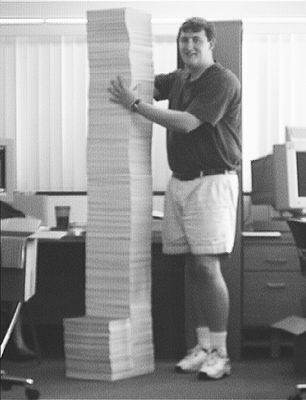
\includegraphics[width=18pc]{gfx/heath-encuestas}\caption[Encuestas trabajo Heath]{Imagen extra�da de \textsc{Heath} \etal \citep{heathMTh}, muestra las 19600 hojas de evaluaci�n impresas de todas las encuestas realizadas.\label{fig:heath-encuesta}}
\end{SCfigure}
\noindent Este uso desmesurado de papel y de tinta es muy poco ecol�gico, por su efectos contaminantes sobre el medio ambiente. Todos estos efectos se acent�an en cuestionarios con im�genes, ya que dichas im�genes han de imprimirse en alta calidad y en alg�n tipo de papel fotogr�fico o, en cualquier caso, de mayor grosor que el papel habitual, y con una gran cantidad de tinta de varios  colores. Tampoco es posible el uso de papel reciclado, ya que los colores y la resoluci�n se ven afectados en este tipo de papel. Todos estos aspectos elevan el coste final del cuestionario. Como ejemplo, en la Fig. \ref{fig:heath-encuesta} se muestra al autor de \citep{heathMTh} fotografiado junto con una columna de papel impreso correspondiente a las 19600 p�ginas de todas las encuestas realizadas para dicho trabajo. Esta imagen muestra gr�ficamente y de manera muy evidente el enorme gasto tanto en papel como en costes de impresi�n que conlleva una evaluaci�n mediante cuestionarios impresos. Adicionalmente, a este tipo de evaluaci�n hay que incorporar otros costes, como es el tiempo empleado en recopilar las respuestas y transcribirlas a una base de datos para su posterior procesamiento.\\
\noindent Frente a la aproximaci�n basada en la impresi�n en papel de los cuestionarios, se encuentra la cumplimentaci�n de los cuestionarios utilizando alg�n sistema Web. La alta calidad de los monitores, con elevadas resoluciones gr�ficas, y la disponibilidad de los cuestionarios en todo momento y en todo sitio con conexi�n a Internet, hacen que los sistemas Web se postulen como una buena soluci�n para enfrentarse a la evaluaci�n de encuestas de tipo multimedia. Por todo lo anterior, para proporcionar soporte a los cuestionarios para la evaluaci�n de la calidad de distintas t�cnicas de procesamiento de im�genes se ha planificado un sistema Web.\\
\noindent Siguiendo las recomendaciones expuestas en este cap�tulo se ha desarrollado una herramienta que permite el dise�o de cuestionarios para la evaluaci�n de contenidos multimedia. A su vez, este sistema facilita la gesti�n de dichos cuestionarios tanto por parte del encuestador para su tratamiento, como de los encuestados para contestarlos. Finalmente, proporciona al encuestador la evaluaci�n de los resultados de los cuestionarios tras aplicarles diversos factores de ponderaci�n.\\
\noindent Esta herramienta ha sido implementada como un sistema Web, para permitir que los encuestados puedan acceder de manera remota a los cuestionarios. De manera adicional, los usuarios pueden interrumpir y retomar los cuestionarios en cualquier momento. Esto es una pr�ctica bastante com�n en pacientes con problemas de visi�n debido al cansancio visual que les acarrea el esfuerzo de ver las im�genes.
\clearpage
\subsection{Preguntas de \textsc{puntuaci�n}}
En la Fig. \ref{fig:wemcas-puntuacion} se muestra un ejemplo de pregunta de \textsc{puntuaci�n} de una encuesta de pilotaje para la evaluaci�n de bordes.\\
\begin{SCfigure}[][!h]
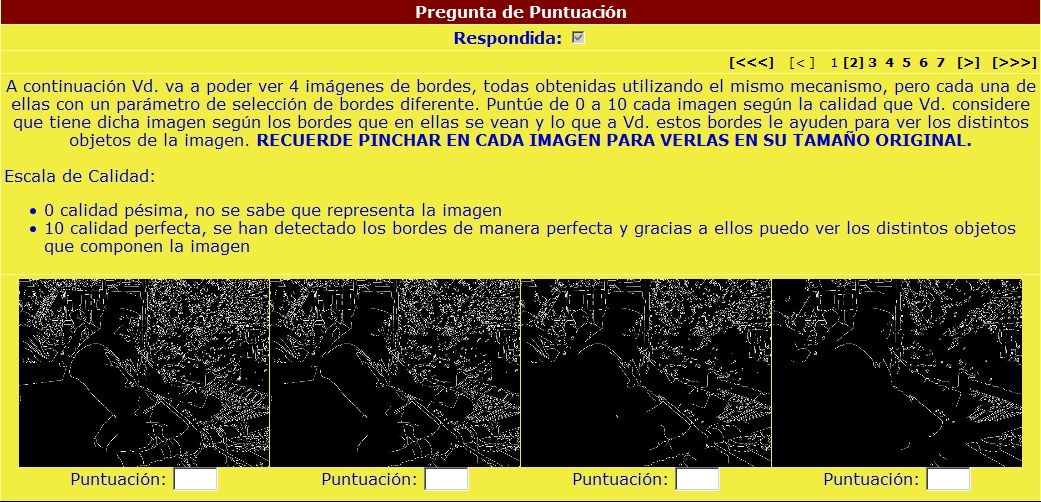
\includegraphics[width=26pc]{gfx/wemcas/wemcas-puntuacion.jpg}\caption[Pregunta de \textsc{puntuaci�n}]{Pregunta de \textsc{puntuaci�n con repetici�n}.\label{fig:wemcas-puntuacion}}
\end{SCfigure}

\noindent N�tese que debajo de cada \emph{imagen respuesta} existe una caja de texto que admite un valor num�rico. Los l�mites inferior y superior de dicho valor se puede parametrizar por parte del encuestador cuando construye el cuestionario, de manera que impida la introducci�n de valores fuera de rango.

\subsection{Preguntas de \textsc{selecci�n sin repetici�n}}
En la Fig. \ref{fig:wemcas-seleccion-unica} se muestra un ejemplo de pregunta de \textsc{selecci�n sin repetici�n} de una encuesta de pilotaje para la evaluaci�n de bordes.
\begin{SCfigure}[][!h]
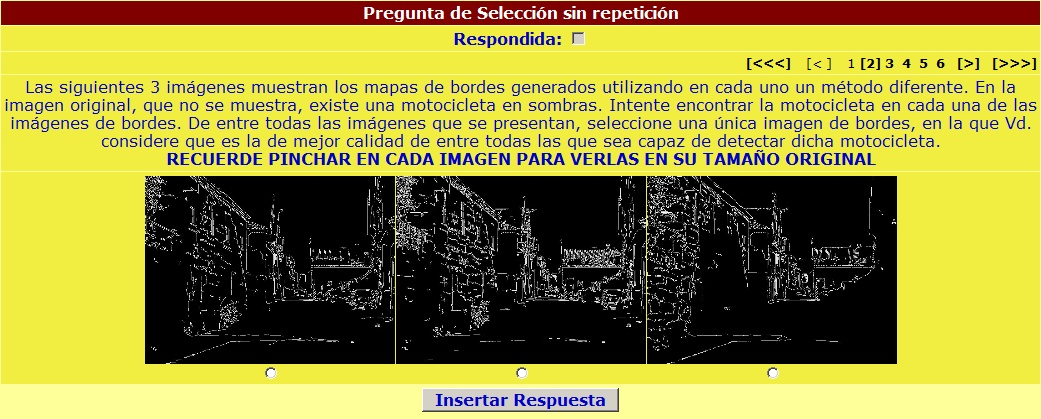
\includegraphics[width=26pc]{gfx/wemcas/wemcas-seleccion-unica.jpg}\caption[Pregunta de \textsc{selecci�n sin repetici�n}]{Pregunta de \textsc{selecci�n sin repetici�n}.\label{fig:wemcas-seleccion-unica}}
\end{SCfigure}

\noindent Debajo de cada \emph{imagen respuesta} hay un bot�n circular que muestra si se ha seleccionado la imagen superior asociada y que, a su vez, s�lo permite que se encuentre activo uno de dichos botones. De tal forma, que si ya hubiese un bot�n seleccionado y se escoge otro bot�n, el primero se desactivar�a y pasar�a a activarse el segundo.
\clearpage
\subsection{Preguntas de \textsc{selecci�n con repetici�n}}
En la Fig. \ref{fig:wemcas-seleccion-repeticion} se muestra un ejemplo de pregunta de \textsc{selecci�n con repetici�n} de una encuesta de pilotaje para la evaluaci�n de bordes.
\begin{SCfigure}[][!h]
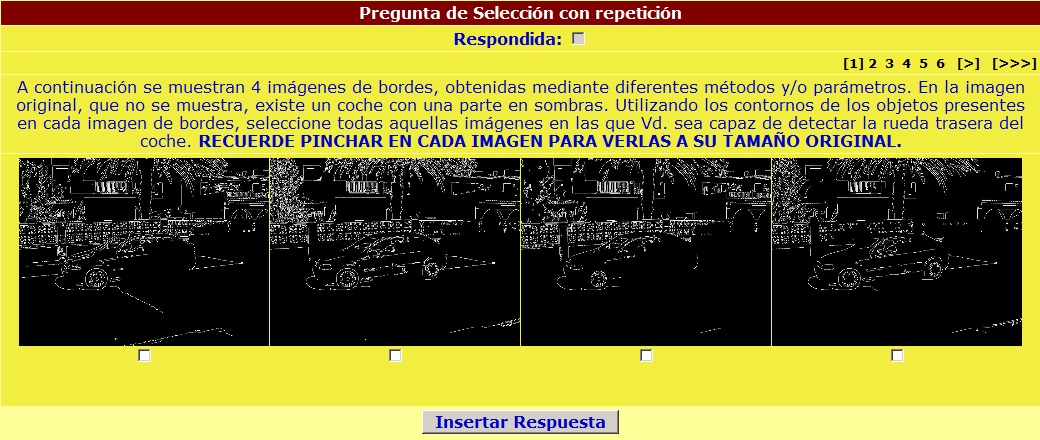
\includegraphics[width=26pc]{gfx/wemcas/wemcas-seleccion-repeticion.jpg}\caption[Pregunta de \textsc{selecci�n con repetici�n}]{Pregunta de \textsc{selecci�n con repetici�n}.\label{fig:wemcas-seleccion-repeticion}}
\end{SCfigure}

\noindent Este tipo de preguntas tienen asociadas a cada \emph{imagen respuesta} un cuadro de verificaci�n, que admite que varios de ellos se encuentren activados simult�neamente.

\subsection{Preguntas de \textsc{mapeado espacial y temporal}}
Finalmente, en la Fig. \ref{fig:wemcas-mapping} se muestra un ejemplo de pregunta con \textsc{mapeo espacial y temporal} de la respuesta para una encuesta de pilotaje para la evaluaci�n de bordes.
\begin{SCfigure}[][!h]
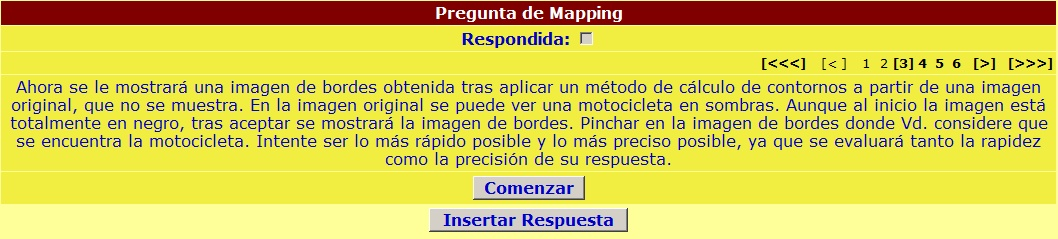
\includegraphics[width=26pc]{gfx/wemcas/wemcas-mapping.jpg}\caption[Pregunta de \textsc{Mapping}]{Pregunta de \textsc{Mapping}.\label{fig:wemcas-mapping}}
\end{SCfigure}

\noindent En este tipo de pregunta se presentan 2 ventanas, la primera, mostrada en la Fig. \ref{fig:wemcas-mapping}, con el texto de la pregunta y un bot�n \emph{Comenzar}, que al pulsarlo muestra la imagen de bordes que se pretende evaluar. Al contemplarse en este tipo de preguntas el tiempo de respuesta, la carga de la imagen se realiza en segundo plano mientras que se muestra el texto de la pregunta. Al pulsar el bot�n de comienzo, se inicia el contador de tiempo y se muestra la imagen precargada en una ventana externa (por lo que para un correcto funcionamiento del sistema hay que desactivar cualquier tipo de software bloqueador de \emph{pop--up}). En dicha ventana, se muestra la imagen y se espera a que el usuario clique con el rat�n en alg�n sitio de la ventana, momento en el que el contador de tiempos se para y se pregunta si se desea almacenar la posici�n marcada como respuesta. En caso afirmativo, se almacena en el sistema tanto el tiempo empleado en cliquear como la posici�n $(x,y)$ de dicha respuesta.
\clearpage
\section{Conclusiones}
\lettrine{E}{n} este cap�tulo se ha analizado el llamado \emph{sesgo por finalidad}, que ha sido identificado como una fuente de distorsi�n en las respuestas de los encuestados y que no se tiene conocimiento de que hubiera sido descrito previamente. Tambi�n, se han propuesto algunas recomendaciones de dise�o de cuestionarios que incorporen elementos visuales dentro de las opciones de respuesta. Estas recomendaciones se han obtenido mediante experimentaci�n y metaencuestas sobre entrevistados que cumplimentaron encuestas de pilotaje. Se ha propuesto un conjunto de tipos de preguntas que facilitan el dise�o correcto de este tipo de cuestionarios. Hay que hacer especial hincapi� en las preguntas con respuestas de \textsc{mapeado espacial y temporal}, ya que son una aportaci�n muy importante que hace esta Tesis para el desarrollo de cuestionarios para evaluaci�n de im�genes.\\
\noindent A pesar de que estas recomendaciones son, en muchos casos de sentido com�n, ser�a conveniente realizar un estudio estad�stico m�s pormenorizado que corroborase cient�ficamente las afirmaciones que se han realizado en este cap�tulo. Este estudio no se ha realizado porque exced�a los l�mites de la presente Tesis, pero desde luego abre un interesante campo de trabajo para futuras investigaciones y tesis doctorales.\\
\noindent Tambi�n es de sumo inter�s, y es otra de las aportaciones importantes de esta Tesis Doctoral, la construcci�n de un sistema Web para la construcci�n de cuestionarios con contenidos multimedia por parte de los encuestadores, y para el manejo y relleno de dichas encuestas por parte de los encuestados.\\
\subsection{Conclusiones de la Parte \textsc{\ref{part:metodoYmateriales}}}
\noindent Con este cap�tulo se finaliza la Parte \textsc{\ref{part:metodoYmateriales}}, \emph{M�todo y Materiales}, en la que se han descrito las aportaciones cient�ficas m�s relevantes de esta Tesis Doctoral. A lo largo del Cap�tulo \ref{chap:convLIP} se describi� matem�ticamente el nuevo operador \emph{Convoluci�n--\textsc{LIP}}, exponi�ndose adem�s dos implementaciones diferentes del mismo, \textsc{DGLIP--Conv} y \textsc{FGLIP--Conv}. En el Cap�tulo \ref{chap:criterios} se especificaron los criterios generales y espec�ficos que se han seleccionado para este trabajo y que han condicionado en gran medida las decisiones de investigaci�n tomadas. Para evaluar los resultados de los algoritmos de extracci�n de bordes dise�ados bajo el modelo \person{LIP} utilizando el operador \emph{Convoluci�n--\textsc{LIP}}, en el Cap�tulo \ref{chap:recCuestCalidadBordes} se han presentado un conjunto de recomendaciones para el dise�o de cuestionarios de evaluaci�n de calidad de bordes. Tambi�n se ha presentado una herramienta Web que ha sido dise�ada expresamente para el dise�o y evaluaci�n de los cuestionarios con contenidos multimedia. El compendio de cap�tulos que forman la Parte \textsc{\ref{part:metodoYmateriales}} es el n�cleo central de esta Tesis Doctoral, ya que en estos cap�tulos se han expuesto las innovaciones cient�ficas. La siguiente Parte \textsc{\ref{part:resultadosExperimentales}}, \emph{Resultados Experimentales}, comenzar� con un cap�tulo en el que se presentar�n experimentos y aplicaciones del nuevo operador propuesto \emph{Convoluci�n--\textsc{LIP}}, comparando los tiempos de computaci�n entre diferentes implementaciones. Tras ese cap�tulo, se mostrar�n los resultados obtenidos a partir del cuestionario de evaluaci�n de im�genes de bordes, tanto para pacientes con \textsc{Baja Visi�n} como para pacientes con un grado de \textsc{Visi�n Est�ndar}.}{\myChapter{Recomendaciones para la Construcci�n de Cuestionarios de calidad de bordes}\label{chap:recCuestCalidadBordes}}
%-----------------------------
\myPart{Experimental Results}\label{part:resultadosExperimentales}
\ifthenelse{\equal{\value{IncluyeCapitulo}}{2}}{%Para empezar, léete lo que he dicho de los otros capítulos - JJ FERGU: Cambiado el titulo
\myChapter{Development of a Service Oriented Architecture for Evolutionary Algorithms}\label{chap:osgiliath}
% Dedicar un capítulo a la implementación es arriesgado, porque una
% implementación no es parte de una tesis, es, bueno,
% implementación. Salvo que justifiques que realmente lo es,
% justifiques las elecciones hechas, deduzcas conclusiones generales,
% presentes una metodología (lo del SOMA ese), en principio, es dudoso
% que necesite un capítulo o incluso que vaya fuera de un apéndice - JJ

%FERGUSON: REESCRITO casi entero para seguir la metodología y borradas un porrón de cosas

%TODO:
% Quitar los "Could be"
\minitoc\mtcskip
\vfill
\lettrine{I}{n} Chapter \ref{chap:soaea} %we presented the services
%that conform an Evolutionary Algorithm  % ¿así, en general? ¿En qué
                                % contexto? - JJ
%and the process to design a service oriented EA. Although the previous
%examples can be developed using any SOA technology, this chapter
%presents OSGiLiath ({\em OSGi Laboratory for Implementation and
%  Testing of metaHeuristics}), an implementation of SOA-EA based in
%OSGi. % lo que hacemos porque... - JJ FERGUSON: comentado todo

IMPORTANTE: Decir que otra de las cosas que ofrece SOA es el auto-descubrimiento de servicios (Y LUEGO USARLO EN EL CAPITULO DE HOMOHETERO)

Previous chapter has presented a methodology to develop SOEAs. This chapter justifies the use of SOA-EA and the steps to create services within it. Solving the questions in each step leads to...

Then, for the implementation and deployment step, we will use a specific SOA technology (OSGi) to implement and deploy all the examples shown in previous sections, and how to accomplish the requirements in the development of EAs and SOA, taking advantage of the capabilities of SOA. As this is an iterative and and incremental methodology, new services can be discovered or removed in next steps (for example, infrastructure services).

\section{Example of creating a service oriented evolutionary algorithm}
\label{sec:soaea:creating}
 
In this example a basic Service Oriented Genetic Algorithm is designed. Then, to illustrate the iterative process of the proposed methodology and the capabilities of using SOA, a NSGA-II algorithm is also designed using the existent services and adding new ones. Finally, new services for 

\subsection{Identification}
As  stated in in Section \ref{sec:distributed:types}, a basic EA is formed by several steps. Solving the questions in Section \ref{subsec:soaea:identification} and the considerations about the design of services (Section \ref{sec:soa:restrictions}) and the genericity of EAs (Section \ref{sec:distributed:design}) a number of abstract services have been identified. In the {\em algorithm domain}, the Algorithm, Population, Parent Selector, Recombinator, Mutator, Replacer, Stop Criterion and Parameters. In the {\em problem domain}, the Fitness Calculator and Initializer. %Finally, a {\em infrastructure domain} service called Asynchronous Enabler, which is in charge of activating new operators when a local optimum is found (for example, no changes in best individual during certain time). FERGU: mover esto al ejemplo de Enabler



\begin{itemize}
\item Algorithm
\item Population
\item Initializer
\item Parent Selector
\item Recombinator
\item Crossover
\item Mutator
\item Mutation
\item Replacer
\item Stop Criterion
\item Fitness Calculator
\item Parameters
\end{itemize}

\subsection{Specification}

 Concrete implementations are defined: {\em N Tournament} and {\em Roulette} are implementations of parent selectors and {\em Optimum Found} the desired stop criterion. Also, to address the problem to be solved, such as {\em MMDP Fitness Calculator} or {\em Binary Initializer}. As we need a fixed set of steps, a {\em Evolutionary Algorithm} service is created to model the flow of services. The discovered services have been specified to accept  a list of individuals. A service to gather all selectors in the environment is used.

  

\begin{itemize}
\item Basic Order
\item Random Mutation
\item NWorst individual replacer
\end{itemize}

\begin{SCfigure}[20][htb]
\centering
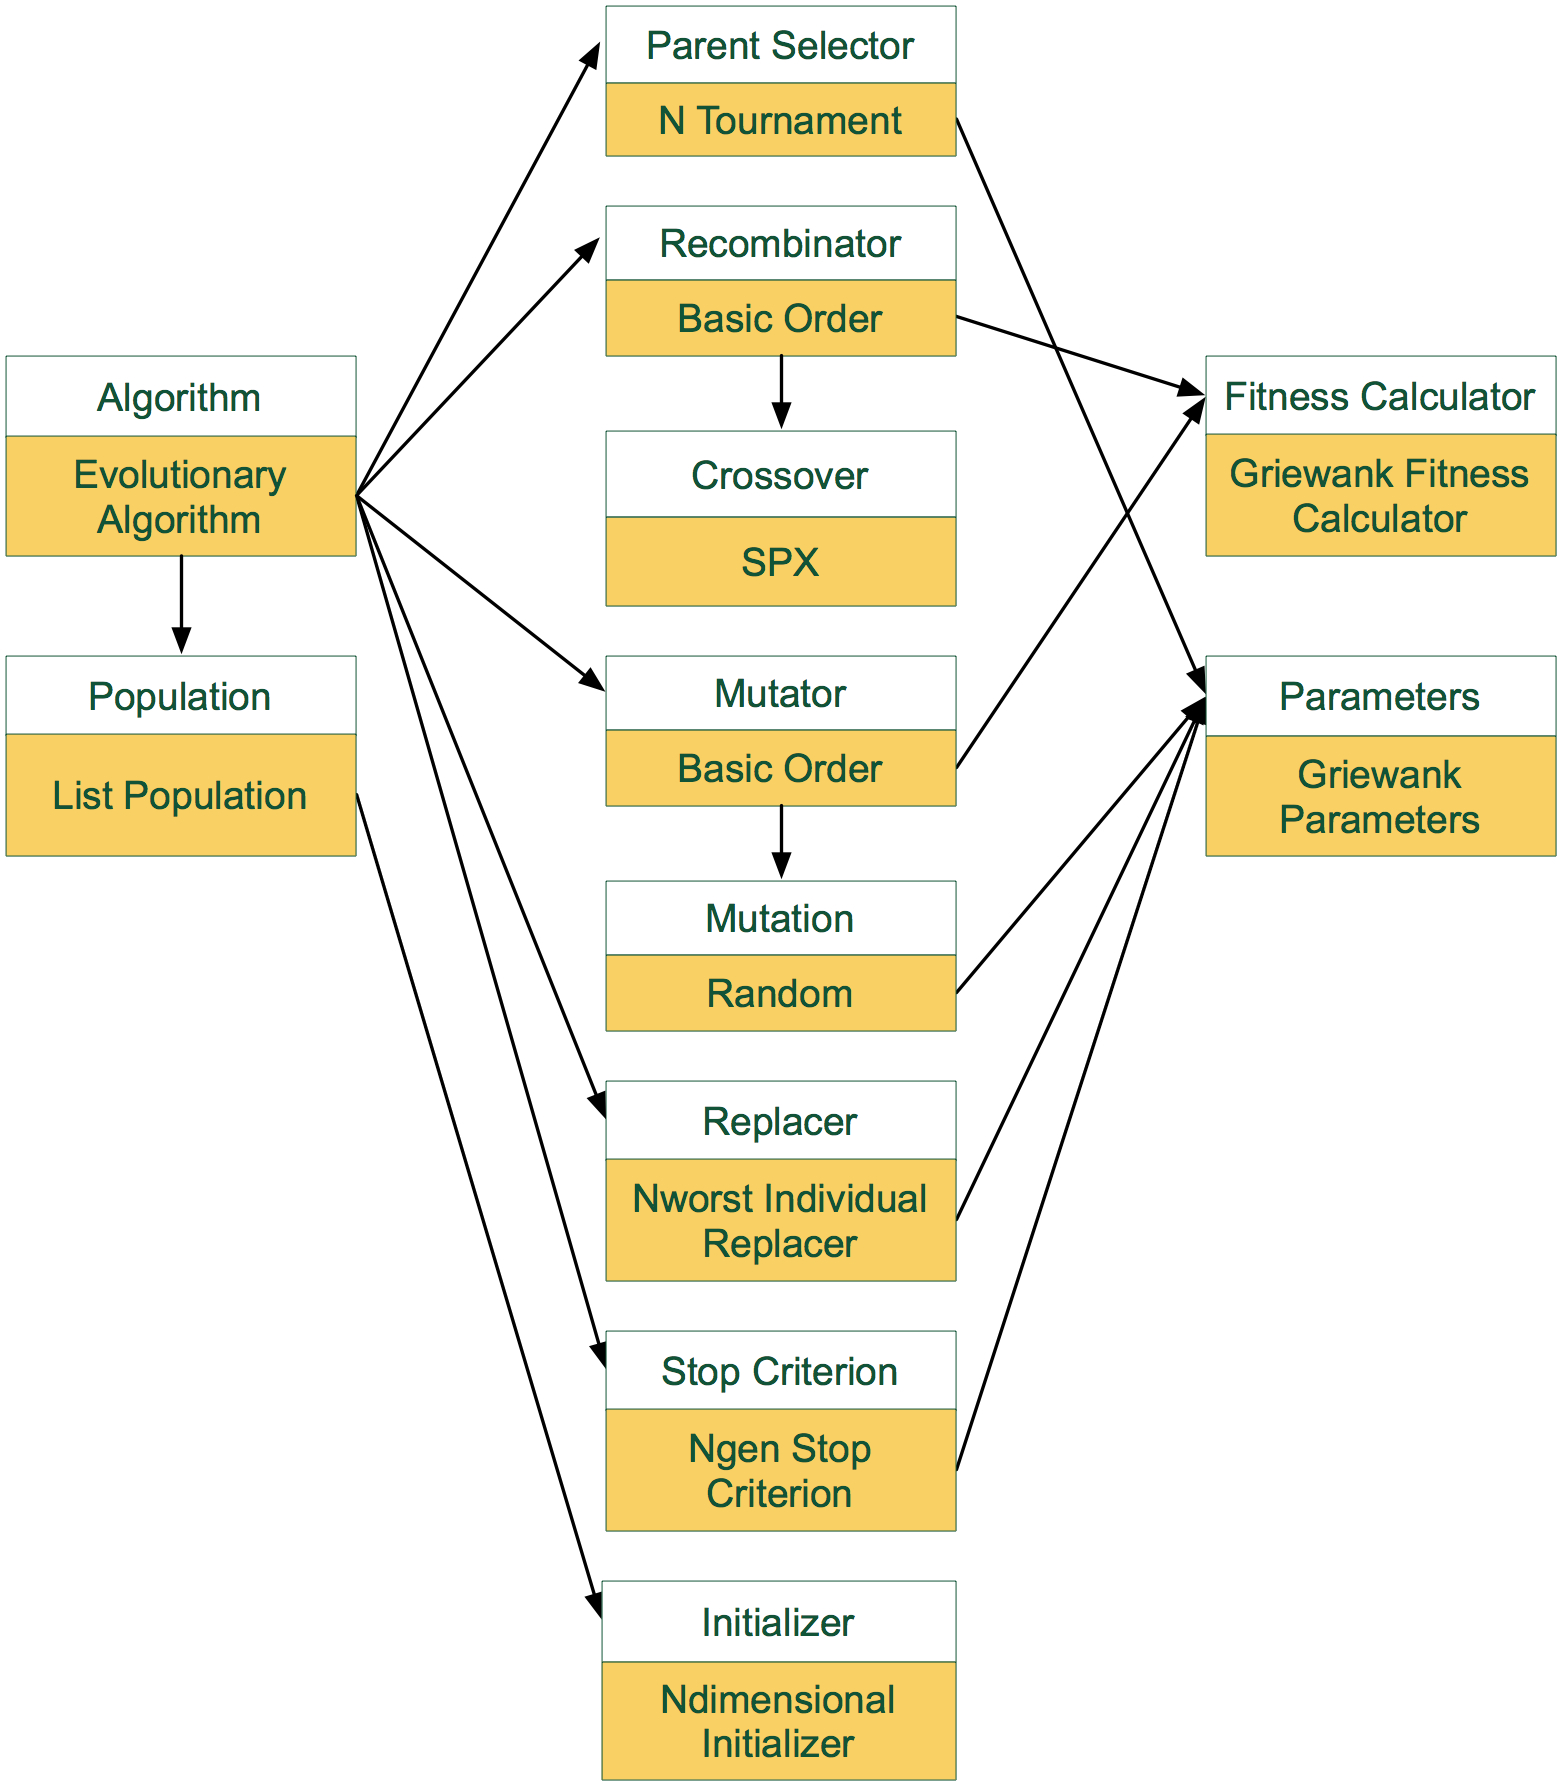
\includegraphics[width=10cm]{gfx/soaea/basicga.jpg}
\caption{Diagram of a basic genetic algorithm. White blocks are interfaces and orange blocks are implementations. In this case, we are using specific implementations to solve the OneMax problem.}
\label{BASICGAEXAMPLE}
\end{SCfigure}





Figure \ref{BASICGAEXAMPLE} shows the diagram of a complete service oriented genetic algorithm, taking into account the proposed ideas. In this figure (and in the following ones) white blocks are the service interfaces. Orange blocks are specific implementations of these interfaces (that is, the source-code of the service), and  arrows indicate how a service implementation can make use of other services via their interface. For example, almost all implementations access to the {\em Parameters} service using its interface. Service implementations (orange blocks) can be selected in a configuration file or be automatically bound when they are available (among other options).



 The change from a problem instance to another is quite simple. It is only necessary to notify the algorithm a change in the implementation of the service {\em Fitness Calculator}. Because some algorithms need to calculate the fitness every time an individual is modified (and not only at the end of a generation) the service {\em Fitness Calculator} may be used inside the implementations that modify individuals ({\em Initializer}, {\em Mutator} or {\em Recombinator}). Moreover, each service can be in the local machine or distributed on the Internet, having the same behaviour. %FERGU: TODO Decir que el fitness se usa solo si hace falta! Arreglado

\subsection{Extending the example to create a NSGA-II}
%\label{sec:nsga2}

As this is a iterative and incremental approach, other services can be discovered and designed in this step. For example, the difference between the previous version of a GA and the well known NSGA-II \cite{NSGA2} lies in the selection operator. Therefore, to change from the basic GA to NSGA-II, the mutator and crossover are kept and new selection operators are added. Figure \ref{fig:nsga2} shows the diagram of the service oriented version of NSGA-II algorithm, where the new implementations are marked with a thick border. The problem has also been changed to Multi-Objective Knacksack problem \cite{MULTIOBJECTIVEKNACKSACK}. New auxiliary services have been added, like {\em Crowding Distance Assignator} or {\em Pareto Assignator}. As these services may be used in other algorithms in the future, they should be designed as abstract as possible. These new services are called from the implementation (code) of the services {\em NSGA-II Replacer} or {\em Binary Crowding Distance Selector} (black arrows indicate an interface call). 




\begin{SCfigure}[20][htb]
\centering
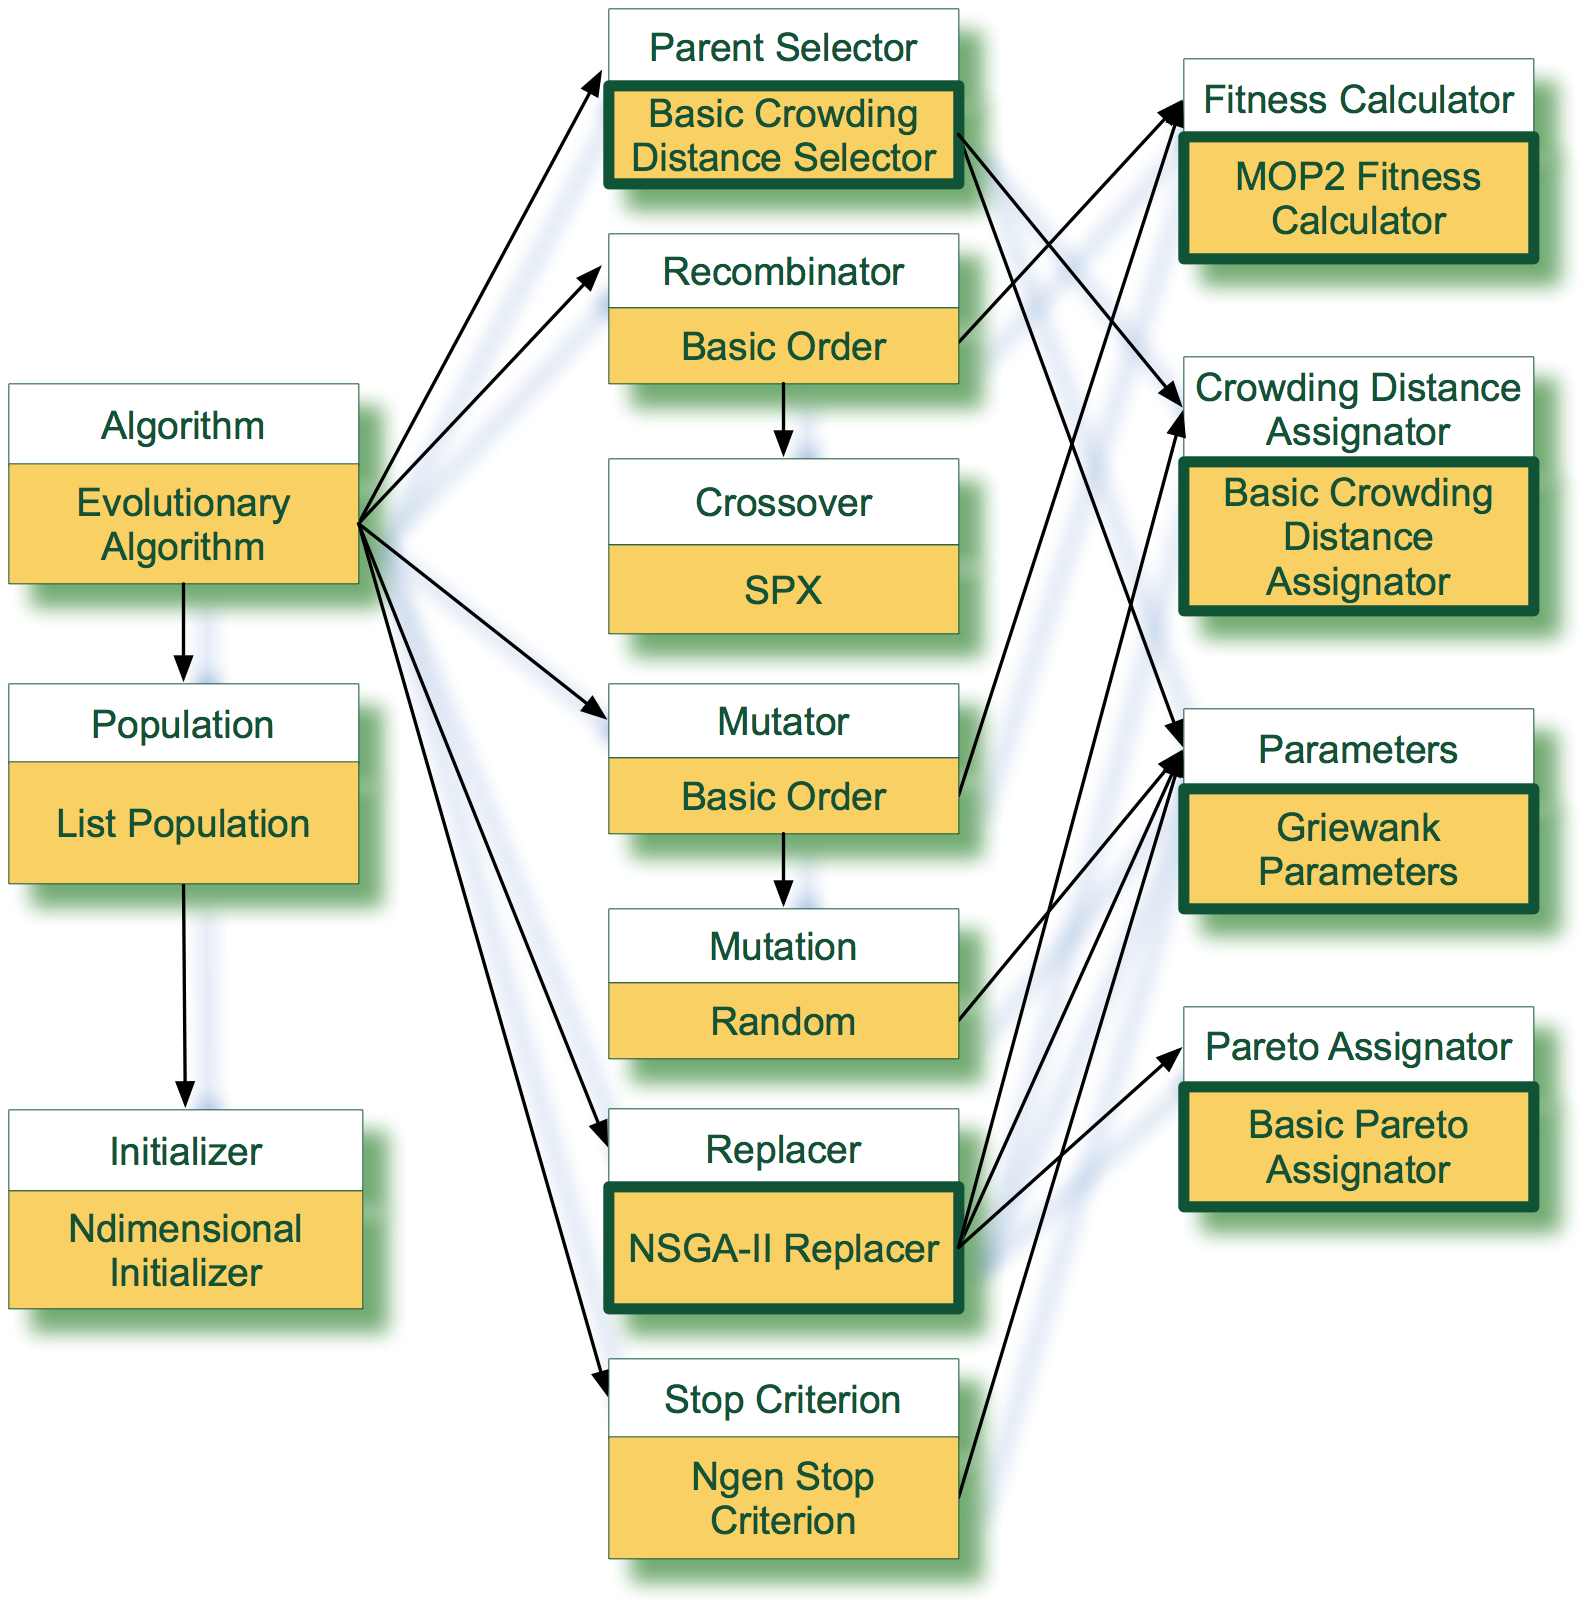
\includegraphics[width=10cm]{gfx/soaea/nsga2.jpg}
\caption{Modification of the basic GA adding new service implementations (orange blocks with thick lines).}
\label{fig:nsga2}
\end{SCfigure}



\subsection{Extending the example to add distribution}
\label{sec:distribution}

As every service must keep the same behaviour, independently of the machine that hosts it, distribution services for load balancing of a specific service can be easily created, for example, notifying the algorithm to use a distributed implementation for that service. As previously stated, the service {\em Fitness Calculator} receives a list of individuals to calculate their fitness, so, in this example, the new fitness implementation ({\em Basic Fitness Distributor}) binds with every fitness service available (in the same machine or in a network). The source code of this basic implementation simply distributes the list of individuals among the bound services and waits for their termination. Although more complex implementations probably will be more efficient, the objective of this section is to show how to distribute services, thus, this basic implementation is sufficient. Figure \ref{FITNESSDISTRIBUTOR} shows the modification from a sequential fitness calculator to a distributed one. Thanks to SOA, the number of distributed fitness calculators is not fixed: calculators can be added o removed in real time without stopping the system. As can be see in the figure, if one of the nodes is a cluster, it could also  implement another fitness distributor. This easy example can be adapted to more complex necessities depending on the infrastructure or the problem to be solved. More complex distribution services can be created, for example, taking into account communication latencies or computation capabilities of the nodes.




\begin{SCfigure}[20][htb]
\centering
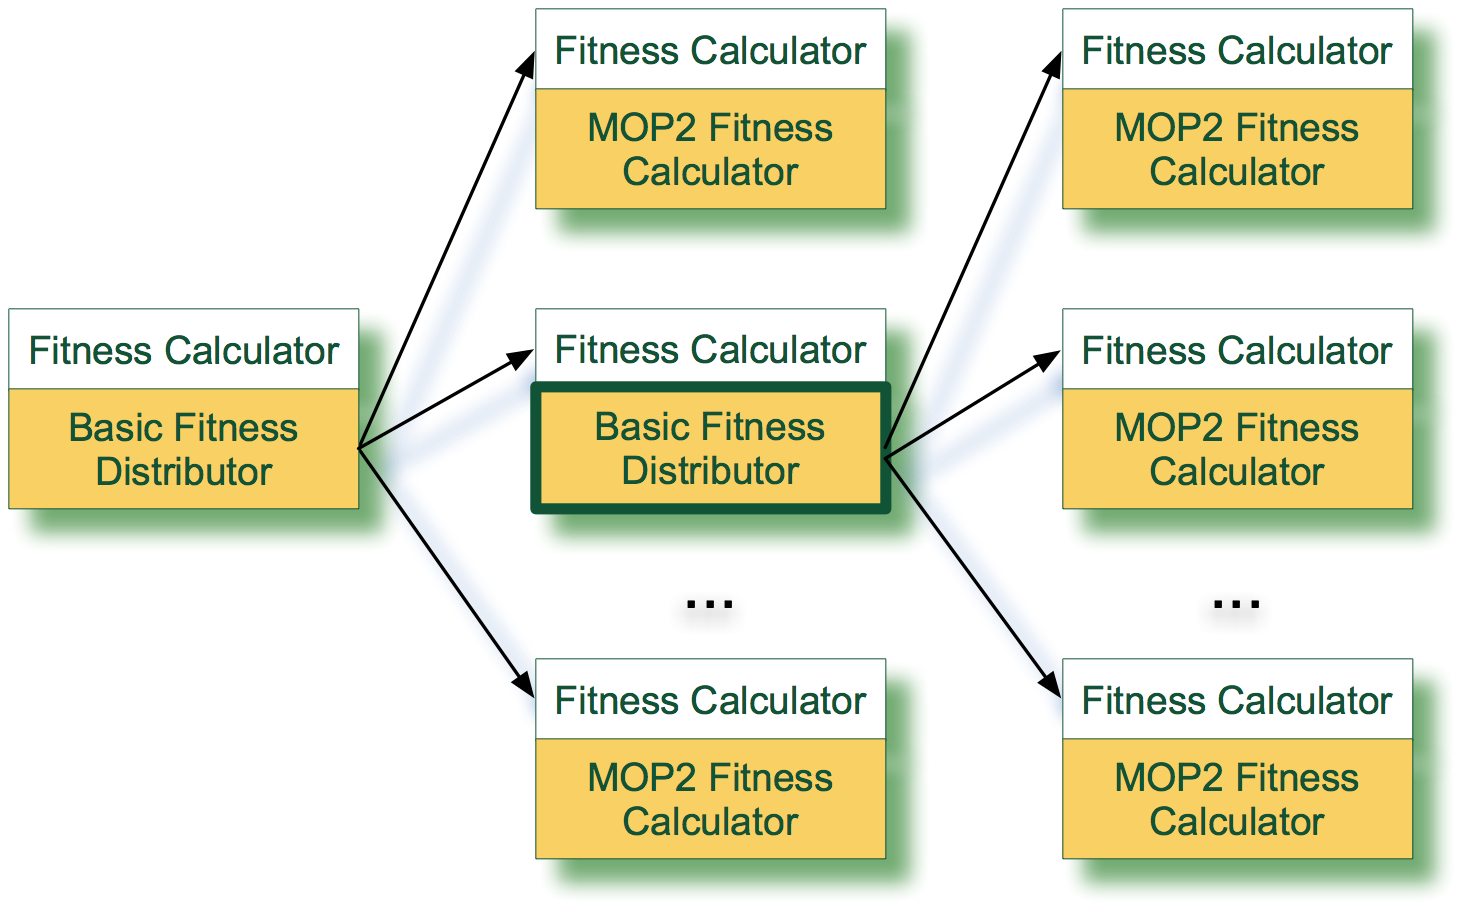
\includegraphics[width=10cm]{gfx/soaea/distributor.jpg}
\caption{Fitness distributor. The thick line implementation also re-distribute the individuals.}
\label{FITNESSDISTRIBUTOR}
\end{SCfigure}



One of the most extended model in parallel EAs is the island model. Using SOA-EA, the {\em Population} service implementation can be modified to become a distributed population. Each certain time, this population could exchange individuals with other populations modified by other algorithms. These populations should be added or deleted in execution time without affecting the algorithm execution. Figure \ref{POPULATION} shows this example, where a {\em Replacer} implementation maintains a list of references to other {\em Population} interfaces (which can be local or remote). Also other {\em Population} implementations exist ({\em List Population} is the usual list of individuals). If one of these population services drop, the others can continue working. The topology of these islands can also be managed from services (such as {\em Basic Replacer} service, or another). The  modification and dynamism of the population structure is difficult to apply in existing frameworks without using SOA because it is necessary to create mechanisms to modify the population behaviour, the operators to modify it, the data structures, and also the code to manage all. With he usage of SOA, and due to the capability of accessing to a population via its service interface, it is not necessary to modify the source code to modify the population and its behaviour. Also, to avoid bottlenecks in distributed executions, asynchronous communication must be provided to avoid idle time. This kind of communication offers excellent performance when working with different nodes and operating systems, as demonstrated by \cite{Alba2002Heterogeneous}.



\begin{SCfigure}[20][htb]
\centering
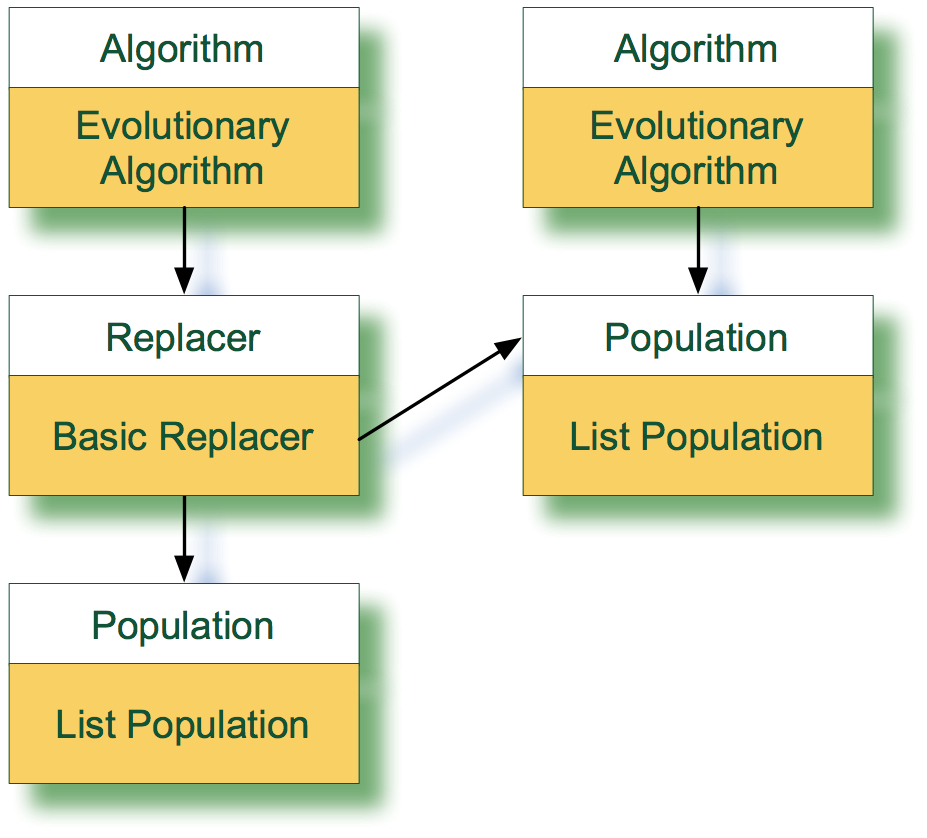
\includegraphics[width=7cm]{gfx/soaea/island.jpg}
\caption{Island model. From time to time, the Basic Replacer Implementation could send or receive individuals from other islands.}
\label{POPULATION}
\end{SCfigure}



\subsection{Self-adaptation of the services}
\label{sec:otherexamples}
There are several ways to create self-adaptable algorithms using SOA. For example, creating a service that modifies the parameters in the {\em Parameters} service, or activating and de-activating operators in real time. An easier way is to create a service that manages all available services of the same kind. For example a {\em Mutator} service that binds all the available mutation implementations and use the most adequate one depending on some rules during the execution \cite{SelfadaptationSerpell2010}.  This idea can also be extended to create a service that implements several interfaces and selects the most adequate implementation for each interface respect to some criteria, as can be seen in Figure \ref{INTELLIGENTALGORITHM}, where thick lines represent the implementations used at the current moment (they vary as time passes).



\begin{SCfigure}[20][htb]
\centering
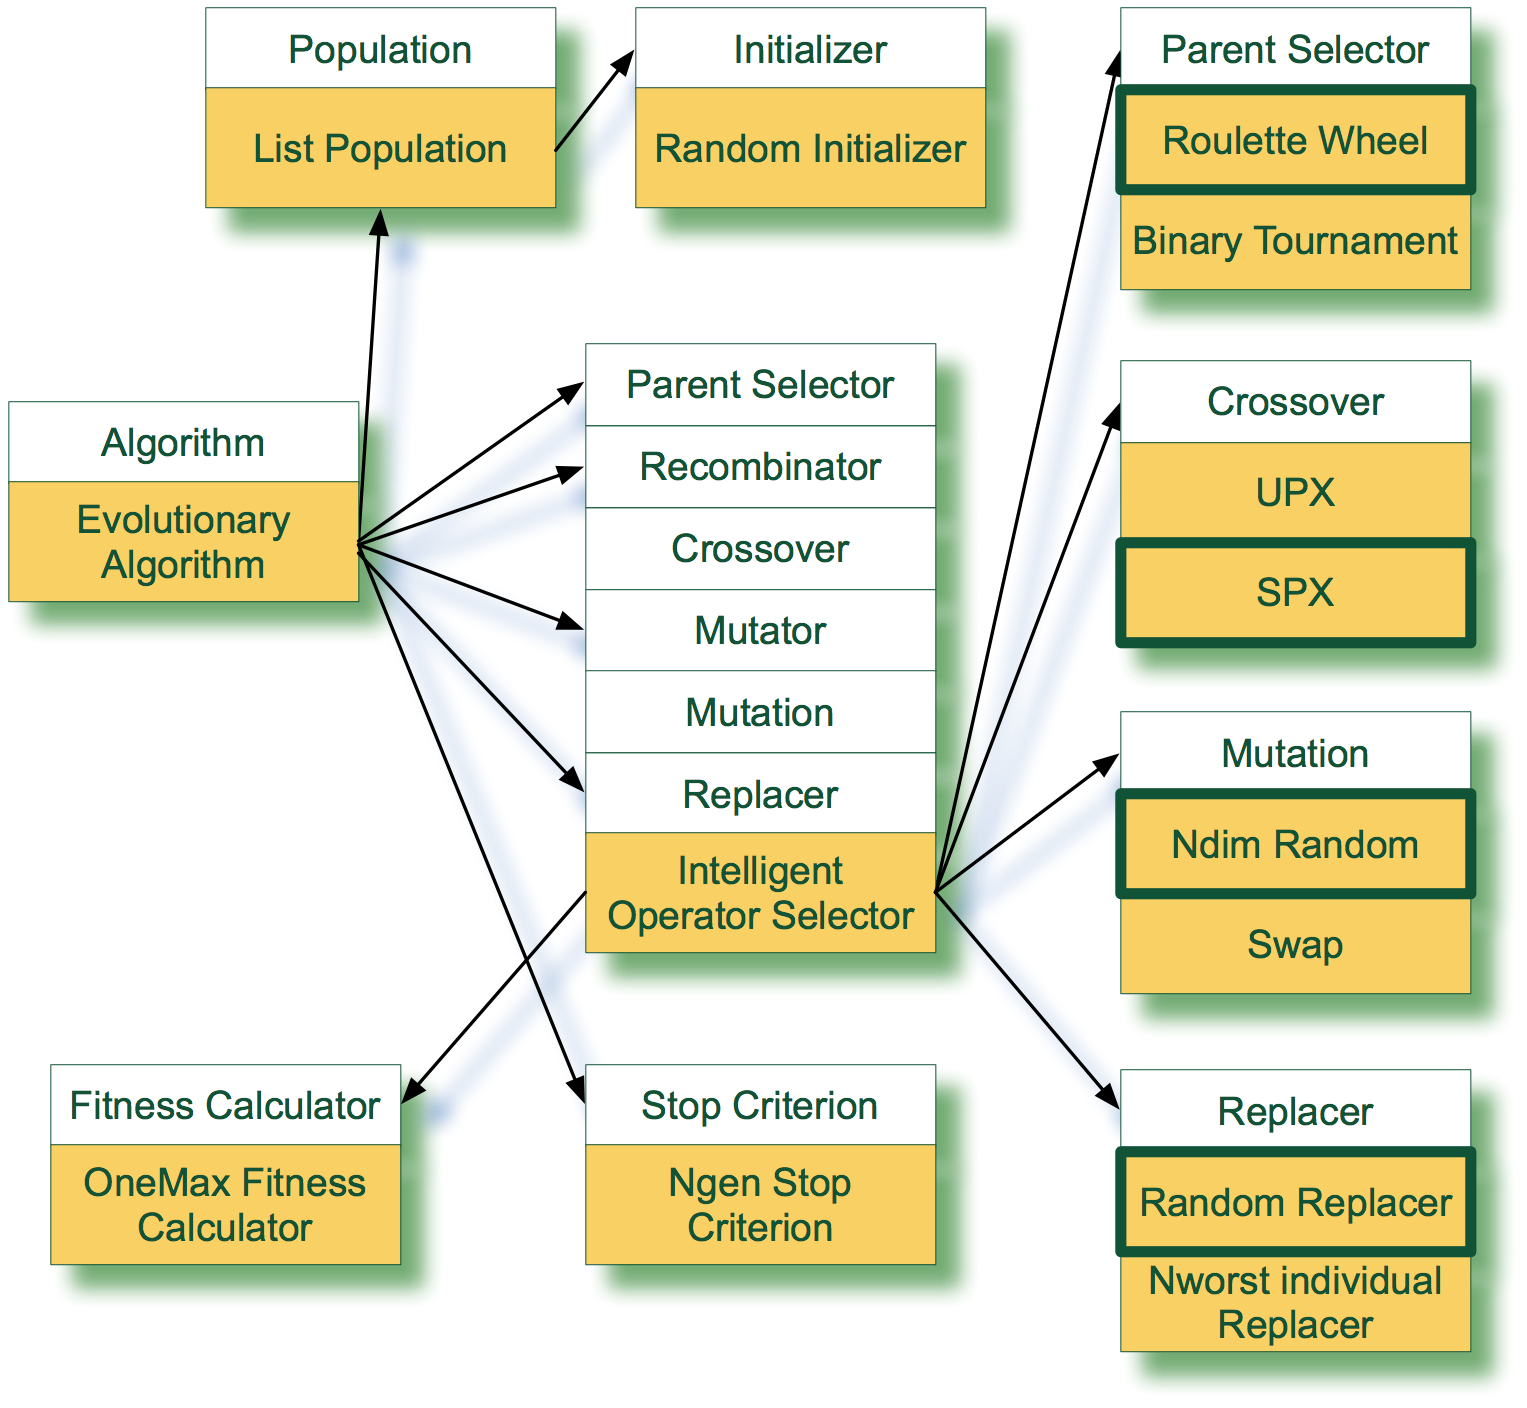
\includegraphics[width=10cm]{gfx/soaea/intelligent.jpg}
\caption{Self-adaptable Algorithm. The {\em Intelligent Operator Selector} selects which service implementation is used each time.}
\label{INTELLIGENTALGORITHM}
\end{SCfigure}


Finally, another important usage of EAs is its hybridization with other metaheuristics, to obtain more effective search algorithms \cite{HybridRodriguez2012},  increasing the performance of intensification and diversification mechanisms. With  traditional frameworks this task can be difficult, mainly because the source code for each metaheuristic must be modified. Nevertheless, using SOA a combination of loosely coupled services could be used.



The questions presented in Section \ref{subsec:soaea:implementation} have been answered to obtain the next restrictions for the desired framework. Initially, the services can be executed locally, they must be dinamically bound and no extra code should be added to allow the distribution of the created implementations. This implementation should allow asynchronous data sending/receiving, without the need to implement
  specific functions in the source code, like MPI or other
  distribution mechanisms. EAs developers can use the existing
  distribution services or create new ones, if they want. New improvements can be added
  without modifying the existing modules, that is, adding or modifying
  only the affected service implementations without modifying the
  source code of the other services.

\section{Implementation and Deployment}

\subsection{Select the technology to use}
\label{sec:osgiliath:technology}

Of the existent technologies for SOA (presented in Section \ref{chap:soa:implementations} Web Services and OSGi have been considered.
% Primero: esto debería ir al principio, incluso en la intro. Segundo
% ¡no uses items! Cuéntalo, nárralo, úsalo como argumento - JJ FERGUSON: Movido y re-escrito (muevo abajo todos tus comentarios juntos)
% ¿Faster que qué? - JJ FERGU: WS
% si no lo vas a usar en tu tesis, eso no
                            % importa nada. No añadas ruido ni razones
                            % espúreas - JJ FERGU: Evorobot
% ¿OSGi no es un
                                % servicio web?  - JJ FERGUSON: No
% Esto tienes que probarlo. No te cuesta trabajo hacer un mínimo
% servicio web para probar qué es mejor; también está el paper de
% Pedro - JJ FERGUSON: TODO
% ¿Seguro que no hay nada parecido en los servicios web? - JJ FERGUSON: 

% esto tendrías que haberlo presentado, en vez de como hechos
% consumados, como una historia. "A la hora de implementar,
% consideramos dos paradigmas diferentes (o tres). Lo que
% necesitábamos, como se dijo bla y bla, era bla y bla. Ergo elegimos
% esto porque tenía bla y bla y el otro sólo tenía bla
% No justifiques
% nada a posteriori, sino a priori, la tesis tienes que construirla,
% no justificarla - JJ FERGUSON: tienes razón, cambiado entero

OSGi has been selected because it is faster than Web Services, because it was designed for 
  lightweight devices \cite{LimGateway08}. Therefore, it can be
  used in embedded devices, like Evolutionary Robotics
  \cite{Garcia2012testing}. On the contrary, as explained in Section \ref{chap:soa:implementations} Web services were created to integrate complex
  data interchange among different companies. This is related with the transmission protocol in web services is SOAP, which implies
  the transmission of an XML ({\em eXtension Markup
    Language}) file \cite{XML}. This file is usually too large (for example, a
  complete list of workers in a company). EAs often need to send
  minimal information, but a large number of times (for example, the
  fitness of several individuals), so a complex transmission protocol
  is not recommended. OSGi includes a lot of mechanisms for data
  transmission, allowing more flexibility depending on the execution environment of
  the algorithms (for example, in a machine, in a local
  network, over the Internet, or even in more lightweight devices). 

Unlike web services, OSGi includes a blackboard event-manager,
   that is, services inform what they are doing without indicating 
 any receiver. Other services can filter this information and actuate
 accordingly, so the synchronization is easier. For example, it is not
 mandatory to create a variable to count the number of times that the
 {\em Fitness Calculator} service is executed: an external service can
 track this number. 

Other reason to use OSGi is the separation between OSGi and the source code of the
   services, so the code of OSGi-based applications can be used in other
   Java-based applications without OSGi. For the same reason,
   frameworks written in Java can be migrated into services in a easy
   way.

Finally, OSGi includes other features that, although they are not related to SOA, facilitate the service development and deployment: version and package
   control, security and life-cycle management of the used
   components, that can be useful in the development of EAs 
   (as explained by \person{Wagner \etal} \cite{WagnerPlugins07}). These advantages can be used by the EA developers if
   they work in a team collaboration. % Pero ¿lo son? - JJ

ECF\footnote{\url{http://www.eclipse.org/ecf/}} has
 been chosen because it is the most mature and accepted implementation
 (claimed by \person{Petzold \etal} \cite{petzold2011dynamic}), % o
                                % sea, que no lo has probado - JJ FERGU: no, lo ha dicho el tipo ese
and it also supports the largest number of transmission protocols,
including both synchronous and asynchronous communication. It provides
a modular implementation of the OSGi 4.2 Remote Services
standard\footnote{\url{http://www.osgi.org/Release4/Download}}. % Una
                                % vez más, NUNCA JUSTIFIQUES A
                                % POSTERIORI. Una tesis es una
                                % descripción de un camino. Quería tal
                                % cosa y tal otra cosa porque eran
                                % importantes para tal y tal
                                % cosa. Estaban tal y tal, pero cólo
                                % cual o pascual tenía lo que yo
                                % buscaba- JJ

ECF includes a number of protocols for service discovery and service providers:
\begin{itemize}
\item Service Discovery API: Includes protocols to announce and discover remote services: Zeroconf, SLP/RFC 2608, Zookeeper, file-based and others \footnote{\url{http://wiki.eclipse.org/ECF_API_Docs\#Discovery_API}}.
\item Remote Service API: Includes protocols to establish the communication (data streams, formats and others): R-OSGi, ActiveMQ/JMS, REST, SOAP, XMPP, ECF Generic \footnote{\url{http://wiki.eclipse.org/ECF_API_Docs\#Remote_Services_API}}. This allows communication with systems that do not use OSGi or Java.
\end{itemize}
% Vale. ¿y? ¿Lo vas a usar luego? - JJ FERGUSON: si, en siguientes capítulos volveré a referenciar esto

More information about the application of OSGi in other areas, with
good practices, benefits and lessons learned is provided by the
authors in \cite{GarciaSanchez2013Gateway}. 



%FERGUSON: He comentado TODO lo que venía ahora
%\section{Framework description}
% no label? - JJ
%This proposed environment is a  framework for the development of
%heuristic optimization applications, not focused on a concrete
%paradigm, and whose main objective is to promote SOA benefits % ¿dónde? - JJ
% and offer these features to programmers: % ¿Por qué? - JJ


%\begin{itemize}
%\item Well defined interfaces. As previously stated, service
%  interfaces have been designed to be as abstract as possible. %¿have
                                %been o will be? ¿Es parte de la tesis
                                %o no? ¿Lo has hecho ya en otro
                                %capítulo? - JJ
%\item Asynchronous data sending/receiving. Due to the distribution
%  capabilities offered by OSGi, the presented implementation allows
%  the direct distribution of services, without the need to implement
%  specific functions in the source code, like MPI or other
%  distribution mechanisms. EAs developers can use the existing
%  distribution services or create new ones, if they want. % En
                                % general, deja claro si esto lo has
                                % deducido tú, es necesario, es una
                                % decisión entre muchas, qué diablos
                                % es y como encaja con TU TESIS - JJ
%\item Service oriented programming. New improvements can be added
%  without modifying the existing modules, that is, adding or modifying
%  only the affected service implementations without modifying the
%  source code of the other services. %¿Esto no lo tiene OSGi de por
                                %sí? - JJ
%\item Server/client or distributed model. All the components of this
%  implementation can communicate in a bi-directional way, so it is not
%  mandatory to use a central server to manage other nodes. % ver
                                % arriba - JJ
%\item Paradigm independent. Although the first developments are focused on EAs, this architecture can be extensible to other kinds of metaheuristics.
%\item Remote event handling. Users can handle a
%  powerful synchronization tool among distributed services using OSGi
%  features.  % ein? - JJ
%\end{itemize}

%\subsection{OSGiLiath organization}

%By now, OSGiLiath counts with the next bundles: %No es un manual. Es
                                %una tesis. Cuenta por qué tiene esos
                                %bundles, qué te ha llevado a
                                %hacerlas, etc etc. ¡Una tesis es una
                                %tesis! - JJ FERGUSON: Comentado (mover a un apéndice?)


%\begin{itemize}
%\item osgiliath: This is the core bundle. It includes all the interfaces common to the algorithms such as {\em Algorithm}, {\em AlgorithmParameters} or {\em Problem}. 
%\item Evolutionary Algorithm:  Includes the {\em EvolutionaryAlgorithm} implementation and interfaces to create the rest of the services that form an EA: {\em Recombinator} and {\em Crossover}, {\em Mutator} and {\em Mutation}, {\em StopCriterion} or {\em FitnessCalculator}. It also provides interfaces for the creation of individuals: {\em Individual}, {\em Fitness}, {\em Gene}, and {\em Genome}. 
%\item Basic Evolutionary Components: Includes several implementations (the most common ones) of the previous interfaces: {\em ListPopulation}, {\em ListIndividual}, {\em DoubleFitness}, {\em NGenerationStopCriterion}, {\em BasicOrderRecombinator}, {\em UPXListCrossover} and others.
%\item Binary Problems: Includes implementation of well-known problems, such as OneMax and MMDP: {\em OneMaxFitnessCalculator}, {\em MMDPFitnessCalculator} or {\em BinaryProblemRandomInitializer}.
%\item Function Problems: Multi-dimensional optimization functions, such as Griegwank or Rastrigin are implemented in this bundle, with their associate Initializers or Fitness Calculators.
%\item NSGA2: Interfaces and implementations of services for the NSGA2 algorithm.
%\item OSGiLiART: Service implementation for the creation of Evolutionary Art: {\em ArtisticIndividual} or {\em HistogramFitnessCalculator} are examples.
%\item NoOSGi: Because OSGi allows the separation of source code with the OSGi framework capabilities, this bundle includes Java code to integrate the services without any specific technology (just using basic Object Oriented programming).
%\item IntelligentManager: An example of how the services can be bound/unbound in real-time. By now, in each step the {\em IntelligentRandomManager} selects randomly from the available Crossovers, Mutators and Replacers implementations.
%\end{itemize}

% ¿Todo esto es interesante para entender tu tesis? 99% de
% probabilidad de que la respuesta sea NO. Así que bórralo
% (posiblemente, como dije al principio, el capítulo entero) - JJ FERGU: borado




%The source code of OSGiLiath is available in
%\url{http://www.osgiliath.org} under a GNU/GPL license. This code is
%an updated version of the work published in
%\cite{GarciaSanchezDistributed2010}.  % Esto deberías justificarlo
                                % también - JJ

 
\subsection{Implementing the services}
\label{sec:osgiliath:implementing}
%Users have to define three elements to add a new service in OSGiLiath:
% NO ES UN MANUAL. "To easen the development of new evolutionary
% algorithms with OSGILIATH, the application interface has been
% designed so that... " - JJ

In OSGi, the services are formed by the next elements:

\begin{itemize}
\item {\em Service interface}. It is a Java interface. The user just needs to specify the operations that the service will perform.
\item {\em Service implementation}. The programmer just writes the code of the interface methods.
\item {\em Service description}. It is an XML file that indicates which
  interface is being implemented and which other services needs to be
  activated. 
\end{itemize}
These concepts are explained in detail in Appendix \ref{chap:appendixosgi}. % ¿Dónde? Etiqueta secciones para poder referirte a ellas - JJ FERGU: movido al apendice

In this step the interfaces of the services identified in
Section \ref{sec:soaea:creating}, such as {\em Algorithm}, {\em
  StopCriterion}, {\em Population} or {\em Recombinator} are implemented in Java. These
interfaces are grouped along other interfaces that do not need to be a
service. For example, the interface of the object {\em
  Individual}. This interface is used in the {\em Recombinator}
interface, which receives a list of {\em Individual} objects to be
recombined, and returns another list with the recombined ones. 
Also, several implementations are included, like {\em
  EvolutionaryAlgorithm} (implementing {\em  Algorithm}) or the rest
of  services explained in previous chapter, like the services for
NSGA-II. % Para que... ¡no describas, justifica! ¡¡¡¡Es una tesis!!! - JJ

Then several of these interfaces have been implemented: examples are TPXCrossover or List Population.

Once the services are implemented, the flow of execution must be . In previous chapter the usage of a Evolutionary Algorithm service implementation was proposed. The source code of the method that executes the algorithm in the class
{\em EvolutionaryAlgorithm} (implementation) is shown in Figure
\ref{fig:javaevo}. It includes methods to bind the six references
to the service implementations that are needed: Population ({\em pop}
in the code), StopCriterion, ParentSelector, Recombinator, Mutator,
and Replacer.  % Usa \sc o algún tipo especial para código - JJ 


\newsavebox{\mintedbox} %¿No hay nada para código? ¿Con colorines y demás? - JJ FERGUSON: si, con minted salen colorines
\begin{lrbox}{\mintedbox}
\begin{minipage}{10cm}
\begin{minted}[mathescape,
               linenos,
               frame=lines,
               framesep=2mm]{java}
//References to the implementations to use
Population pop;
ParentSelector parentSelector;
Recombinator recombinator;
Mutator mutator;
Replacer replacer;

//Example of the method to obtain an implementation
//of the ParentSelector interface 
//(one function per reference)
void setParentSelector(ParentSelector sel){
  this.parentSelector = sel;
  //now sel is a reference to an implementation 
        //of ParentSelector
}

//Implementation of the start() method of the 
//Algorithm interface
public void start(){
  pop.initializePopulation();
  actualIteration = 0;
  do{
    //SELECT parents
    List<Individual> parents = 
    parentSelector.select(pop);
      
    //RECOMBINE parents
    List<Individual> offspring = 
    recombinator.recombine(parents);
      
    //MUTATE offspring
    List mutatedOffspring = 
    mutator.mutate(offspring);
      
    //SELECT new population. 
    //pop is modified here
    replacer.select(pop, parents, 
    offspring, mutatedOffspring);
      
    actualIteration++;
      
  }while(!stopCriterion.hasFinished());
    
}
\end{minted}
\end{minipage}
\end{lrbox}
% Hay que tener mucho cuidado con poner código en una tesis porque hay
% gente que puede leérselo. Yo lo quitaría, pero si está, asegúrate
% que sigue todas las buenas prácticas. Por ejemplo, en vez de
% hasFinished debería llamarse "isMet" o
% "isTrue". initializePopulation es repetitivo: debería ser initialize
% simplemente. 
% Es más, estas críticas tendrían toda la razón de ser porque estás
% incluyendo el diseño del framework como parte de la tesis, así que
% deberías seguir todas las buenas prácticas que haya sobre el
% tema. Además, no está el código completo, ¿no? El this de la
% función ¿a qué se refiere? - JJ

\begin{SCfigure}[20][htb]
\usebox{\mintedbox}
\caption{Java code of the class {\em Evolutionary Algorithm}. This class implements the {\em Algorithm} interface, which defines the operation {\em start()} } 
\label{fig:javaevo} 
\end{SCfigure}


%This is the code needed by a EA, so it not necessary to modify it
%(for example, to change from a GA to an ES).  % eso es muy
                                % arriesgado. es un GA canónico, con
                                % un solo operador de mutación y de
                                % crossover, que lo hace exactamente
                                % en ese orden, no usa
                                % elitismo... Decir que no es
                                % necesario modificarlo es discutible
                                % y además no sé qué tiene que ver con
                                % TU TESIS - JJ FERGU: Quitado. En el anterior capitulo puse que era un ejemplo de flujo

\subsection{Deploying the services}

The services are deployed inside an OSGi container (such as Equinox or Felix). The container has mechanisms to list, start and stop services. To automatically bind the service implementations with the service interfaces                                
 the {\em Service Description} is used. % ¿Eso qué tiene que ver
                                % con el código de antes? - JJ FERGU: Añadida frase en medio
Each implementation of a service has an XML file indicating which interface is being implemented, and also other properties. This file is used by OSGi to automatically bind the services. The service descriptor of the EA is shown in Figure \ref{fig:ds}. This file describes that the {\em EvolutionaryAlgorithm} class is an implementation of the {\em Algorithm} interface, and that it needs implementations of the interfaces {\em Population}, {\em Mutator}, {\em ParentSelector}, {\em Replacer}, {\em StopCriterion} and {\em Recombinator} to be activated.

It should be noted that this file usually can be modified using a friendly GUI, or from an assistant in Java IDEs, such as NetBeans or Eclipse (so, users do not have to care about its XML structure). The user interface to create this file in Eclipse is shown in Figure \ref{fig:xmlgui}. The interface being implemented is set in the lower part ({\em Algorithm}). The necessary services to activate this implementation are indicated in the upper part (with the cardinality and functions to set and unset the service implementations in the implementation source code).

\newsavebox{\mintedboxDS}
\begin{lrbox}{\mintedboxDS}
\begin{minipage}{10cm}
\begin{minted}[linenos,
               fontsize=\scriptsize,
               frame=lines,
               framesep=2mm]{xml}
<?xml version="1.0" encoding="UTF-8"?>
<scr:component xmlns:scr="http://www.osgi.org/xmlns/scr/v1.1.0" enabled="false"
immediate="true" name="OsgiliathEvolutionary" >
<implementation class="es.ugr.osgiliath.evolutionary.EvolutionaryAlgorithm"/>
<service>
<provide interface="es.ugr.osgiliath.algorithms.Algorithm"/>
</service>
<reference bind="setPopulation" cardinality="1..1"
interface="es.ugr.osgiliath.evolutionary.elements.Population"
name="Population" policy="static" unbind="unsetPopulation"/>
<reference bind="setMutator" cardinality="1..1"
interface="es.ugr.osgiliath.evolutionary.elements.Mutator"
name="Mutator" policy="static" unbind="unsetMutator"/>
<reference bind="setParentSelector" cardinality="1..1"
interface="es.ugr.osgiliath.evolutionary.elements.ParentSelector"
name="ParentSelector" policy="static" target="(selectorName=nsga2)" 
unbind="unsetParentSelector"/>
<reference bind="setReplacer" cardinality="1..1"
interface="es.ugr.osgiliath.evolutionary.elements.Replacer"
name="Replacer" policy="static" target="(replacerName=nsga2)" 
unbind="unsetReplacer"/>
<reference bind="setStopCriterion" cardinality="1..1"
interface="es.ugr.osgiliath.evolutionary.elements.StopCriterion"
name="StopCriterion" policy="static" unbind="unsetStopCriterion"/>
<reference bind="setRecombinator" cardinality="1..1"
interface="es.ugr.osgiliath.evolutionary.elements.Recombinator"
name="Recombinator" policy="static" unbind="unsetRecombinator"/>
<property name="algorithmName" type="String" value="EvolutionaryAlgorithm"/>
</scr:component>
\end{minted}
\end{minipage}
\end{lrbox} % ¿En serio que merece la pena meter estos tochos? JJ

\begin{SCfigure}[20][htb]
\usebox{\mintedboxDS}
\caption{Service descriptor of the Evolutionary Algorithm implementation.  Figure \ref{fig:xmlgui} shows the friendly user interface to automatically create this file using the Eclipse program} 
\label{fig:ds} 
\end{SCfigure}

\begin{SCfigure}
\centering
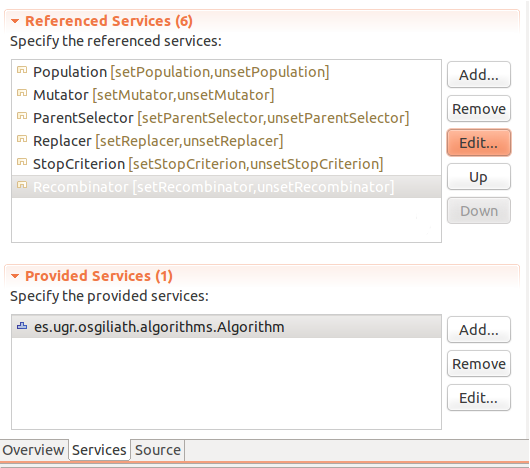
\includegraphics[width=8cm]{gfx/osgiliath/eclipse.png}

\caption{Graphic user interface in Eclipse that generates the Service Descriptor of Figure \ref{fig:ds} }.
\label{fig:xmlgui}
\end{SCfigure}



This XML file is read by the OSGi execution environment, which is the
responsible to bind the available services to this implementation. For
example, if a {\em ParentSelector} is activated, automatically is
bound to the variable {\em parentSelector} through the function {\em
  setParentSelector}. The {\em cardinality} is also set in the file,
in this case, only one implementation is necessary (not
multiple). This file can be modified in execution time, so it is not
required to re-compile the Java code to use and set new services. % zzzzzzzzz interés para la tesis: 0 - Jj

In brief, each implementation of a service (\textit{$<$im\-ple\-men\-ta\-tion$>$}) indicates the interface to being implemented (\textit{$<$pro\-vi\-de in\-ter\-fa\-ce$>$}), and the other services this implementation needs (\textit{$<$re\-fe\-ren\-ce$>$}). 

Moreover, each service can provide properties to be used by other
services to obtain more information and filtering. For example, in
this case only the {\em Replacers} whose property {\em
  replacerName=nsga2} are used. 


\subsection{Managing services: implementing the NSGA-II from the canonical GA}

Following the development example showed in Section \ref{sec:nsga2},
some extra services have been developed to convert the basic GA into a
NSGA-II %(and have also been added to OSGiLiath to be available for
%users). % ¿Lo ves como lo de arriba no incluía todos los GAs? - JJ Bueno, en teoría NO he modificado el código del EA, sólo he añadido servicios nuevos

There exist many options for the implementation of the EA to pick up the appropriate
service. % ¿El EA elige las opciones? - JJ FERGU: arreglado
 The first of them is modifying the source code of the
 implementations. Obviously this is not recommended, because the
 service would not be loosely coupled due to the specific OSGi code,
 and this is not a good SOA practice. The following ways makes the
 service usage not code-dependent: 

% No describas el ejemplo. Crea una metodología para implementar
% algoritmos y aplícala a casos particulares. Esto debería ser un
% ejemplo de una metodología más general. En la tesis no se cuenta lo
% que uno ha hecho, se cuenta la metodología que ha desarrollado uno
% para que otros puedan usarlo también. Supón guq te llega alguien y
% te dice "¿Cómo implemento un EDA?" ¿Le cuentas como se implementa
% NSGAII y que se apañe? - JJ FERGU: bueno, pues al final hice la metodología :)

\begin{itemize}
\item De-activating the implementation {\em Binary Tournament} from the OSGi administration console, and activating the implementation {\em Crowding Distance Selector} (that is, manually). This technique is not recommended, because all services are then managed by hand, and this is very difficult with a large number of services. However, the OSGi console allows modifying services in execution time, so it can be used in some cases (for example, to stop the service in a machine while another big task is being executed, and activate it again when this task is over).
\item Modifying the Service Descriptor of the {\em Evolutionary Algorithm} implementation to filter the desired implementations (for example, the attribute {\em target\-=``(selectorName\-=nsga2)''} in Figure \ref{fig:ds}). This option is used when the algorithm is fixed and does not need to be modified in execution time, and the number of operators and types are known in advance. However, as previously stated, new services can be added in execution time (for example, if the cardinality is set to multiple).
\item Using an external service that activates or de-activates desired implementations or modify their status. This technique must be used when self-adaptation properties are used in the algorithm, and it is presented in next subsections. 
\end{itemize}


None of these options needs to modify the source code of the existing
services: they just indicates which services uses each time.
% ¿Y no será más fácil tener varias implementaciones de referencia, una
% de ellas multiobjetivo como NSGAII? - JJ
% Ferguson: La cosa es elegir entre las que tienes (incluida esa)

\subsection{Making it distributed}
\label{sec:osgiliath:distributed}
% ¿Por qué no pones etiquetas de sección ? - JJ FERGU: añadida

As previously stated in the introduction of this chapter, services should be undistinguishable of being local or remote, and not to add extra code for distribution. Therefore, all services
can be distributed using the OSGi features. In this case, the
distribution is performed using the service descriptor to set which
service is distributable and which is the distribution technology that
provides service discovering and data transmission. 

As explained in Section \ref{sec:osgiliath:technology}, %¿qué sección? - JJ FERGU: Done
 OSGi allows several implementations for the service
 distribution. 
 This specification uses the OSGi service registry to expose remote services to other machines (being indistinguishable from the local ones).  ECF also separates the source code from the discovery and transmission mechanism, allowing users to apply the most adequate technology to their needs, and providing the integration with existing applications. For example, the lines of Figure \ref{fig:remote} have been added to the service descriptor of {\em MOP2 Fitness Calculator} to distribute it in the local network.

 





\newsavebox{\mintedboxServer}
\begin{lrbox}{\mintedboxServer}
\begin{minipage}{10cm}
\begin{minted}[linenos,
               fontsize=\scriptsize,
               frame=lines,
               framesep=2mm]{xml}

<property name="service.exported.interfaces" type="String" value="*"/>
<property name="service.exported.configs" type="String" 
value="ecf.generic.server"/>
<property name="ecf.exported.containerfactoryargs" type="String" 
value="ecftcp://localhost:3787/server"/>
\end{minted}
\end{minipage}
\end{lrbox}

\begin{SCfigure}[20][htb]
\usebox{\mintedboxServer}
\caption{Lines added to the service descriptor of Figure \ref{fig:ds} to be discovered by other services in a network  (this can also be done in the GUI)} 
\label{fig:remote} % Conque digas que sólo hay que añadir cuatro
                   % líneas es suficiente, no hace falta que pongas el
                   % XML - JJ
\end{SCfigure}

In this case, it is only necessary to set the properties that ECF uses
to identify the services being distributed in the network, indicating
that all implemented interfaces are distributable
(\texttt{ser\-vi\-ce\-.ex\-por\-ted\-.in\-ter\-fa\-ces}). Also, the
communication technology to be used is established
(\texttt{ecf\-.ge\-ne\-ric\-.ser\-ver}, although another kind of
protocol could be used), and finally, the service URL (\texttt{
  ecf\-.ex\-por\-ted\-.con\-tai\-ner\-fac\-to\-ry\-args}). As
previously stated, the service properties can be modified from other
services, so these properties  % THESE properties!!! - JJ
can be added outside the XML. It should be noted that the source code
of the services has not been modified to distribute them (as would
happen if MPI had been used to perform the distribution, for
example). % Pues pon como requisito desde el principio que eso es lo
          % que buscas y por eso has elegido ECF en vez de MPI o lo
          % que sea - JJ FERGUSON: añadido al principio

%\subsection{Example of programming an island model} %Sin leerlo ya te
                                %digo que lo elimines. ¿Qué quieres
                                %probar aquí? ¿Qué información añade a
                                %la tesis? FERGUSON quitado entero y reescrito en otro capítulo






%Aquí, más perdido que el barco del arroz. Todo esto parece como el
%algoritmo del tirador bizco: tiro a todos lados y acabo dando. En vez
%de hablar de implementación, tienes que hablar 
% 1. El camino que te ha llevado a usar este tipo de implementación y
% no otra y por qué has desechado los otros, incluyendo experimentos y
% referencias a "implmentation matters".
% 2. Si alguien quiere desarrollar algo nuevo, qué es lo que tiene que
% hacer. ¿Crear nuevos intelligent manager? ¿Nada? ¿Tocar las
% descripciones de servicio? 
% 3. Desarrollar, paso por paso, una implementación de algo (si puede
% ser algo que no hayas publicado todavía) y mostrar lo fácil que es,
% el poco esfuerzo necesario y las pocas líneas de código que hacen
% falta. 
% Y todo esto te lo he dicho desde el día 1. Que conste - JJ
% FERGU: reescrito todo para que cumpla los puntos




\section{Experiments} %¿Implementation o experiments? ¿Estamos a setas
% o estamos a Rolex? - JJ FERGU: Puesta frase. TERMINA
In this section, several experiments to confirm some of the advantages of using SOA and OSGi, explained in previous sections, are proposed. First, a comparison of time of using OSGi and the services as normal classes is presented to demonstrate that OSGi does not adds extra overhead (as explained in Section \ref{subsec:soa:osgi}). Experiments to demonstrate the automatic adding of new operators during runtime, and integration with other systems without modification of the existent source code are shown. Finally, a comparison of Lines of Code (LoCs) with other existent frameworks for EAs (presented in Section \ref{subsec:soaea:fworks}) is performed.

\subsection{Comparing overhead of using services}
One may think that working with services usually implies an
overhead. This is true when communication protocols like SOAP are
used, because the transmitted XML must be generated and
parsed. However, as SOA is independent of the implementations,
services also can behave as normal method calls in the same machine. 


%The first experiment of this section is focused on this issue, % ¿Qué
                                % issue? No has dicho ni qué quieres
                                % probar. Ni por qué es importante
                                % para la tesis. Ni nada. Si se trata
                                % de que OSGi no es más lento que una
                                % implementación local, tendría que
                                % haber ido al principio (y el
                                % capítulo llamarse OSGi
                                % implementation of evolutionary
                                % algorithms and its applications) - JJ
%and will demonstrate that the use of a SOA oriented % ¿a service
                                % oriented aplication oriented
                                % implmentation? - JJ
%implementation of an EA does not %nunca uses apóstrofos en lenguaje
                                %formal!!!!! - JJ
 The basic GA implemented in Section \ref{sec:osgiliath:implementing} is also executed outside of
 the OSGi framework, and a normal Java class has been used to
 integrate the interfaces and implementations ``as is''. The
 population has been set to 64 individuals, parents have been selected
 using Binary Tournament, and the mutation rate has been fixed to
 0.1. % ¿Esto influye en el resultado? Si influye, ¿has probado varios
      % settings? Si no, ¿para qué lo mencionas? - JJ FERGU: bueno, es por reproducibilidad de resultados
Worst individuals (parents and off-spring combined) are replaced, and
the stop criterion has been set to 200 generations. Each experiment
has been launched 30 times to solve the OneMax problem
\cite{SchafferOnemax91}. 

\subsection{Adding operators in runtime for self-adaptation} % ¿Una subsección? ¿Seriously? ¿Y con un párrafo? - JJ FERGU: cambiado el nombre, reescrito y movido de sitio todo lo que había

Previous sections remarked that using SOA benefits are also related
to self-adaptation. A simple example is presented here to demonstrate
how easy is to convert a basic evolutionary algorithm into a
self-adaptive one in OSGiliath. 
%In this example, an intelligent service manages all the available operators. In this case, the service {\em IntelligentRandomManager} implements the interfaces {\em Parent  Selector, Recombinator, Mutator} and {\em Replacer}. All operator implementations previously presented are added to the Manager during  runtime (see Figure \ref{INTELLIGENTALGORITHM}) when they become activated in the system. Every time the EA calls an operator, this simple manager chooses randomly one of the available implementations it controls. % ¿Eso es auto-adaptativo? Es más, para
                             % lo que haces, ¿no hay forma de hacerlo
                             % a otro nivel sin necesidad de crear un
                             % nuevo Intelligent Manager? - JJ FERGU: Borrado y puesto un experimento nuevo

                             % Me he quedado igual. ¿Ha servido esto de algo? ¿Dónde está el
% ejemplo? ¿Funciona el algoritmo mejor? - JJ FERGU: Añadido el experimento abajo, reescrito

Infrastructure services to deal with control of the population and to enable other operators are also implemented (Asynchronous Enabler Imp). Figure \ref{fig:osgiliath:enabler} shows this designed configuration.

To demonstrate that services can be managed and deployed during runtime a simple experiment is proposed. A external service to the algorithm runs in parallel consulting the population from time to time. If the best individual has not been improved in a number of times this service automatically enables another implementation of Parent Selector. This new implementation is automatically bound by the the {\em Selector Gatherer} service and start to use it. Figure \ref{fig:osgiliath:enabler} shows this configuration.

\begin{SCfigure}[20][htb]
\centering
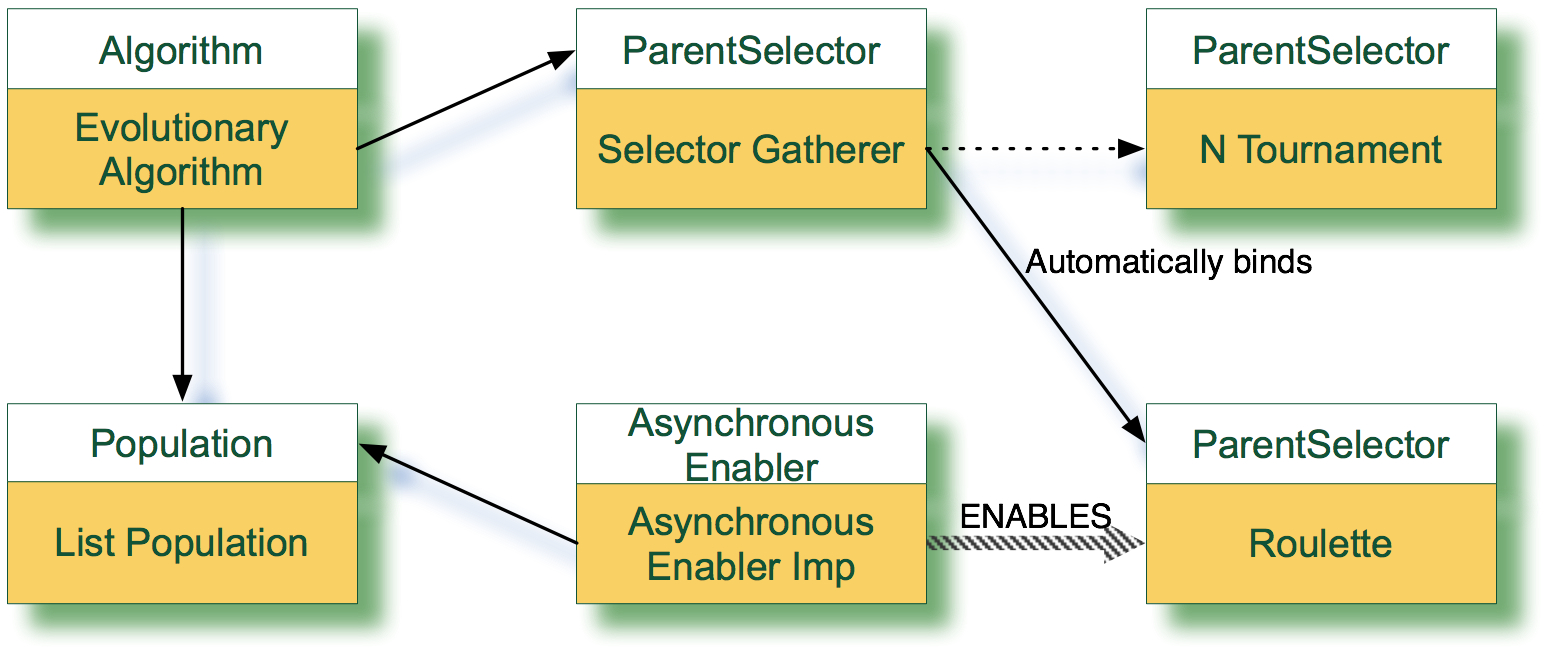
\includegraphics[width=10cm]{gfx/osgiliath/enabler.jpg}
\caption{Service that enable automatically an operator to be used during runtime.}
\label{fig:osgiliath:enabler}
\end{SCfigure}

This enabler does not affect the code of the existent services (such as Population or Evolutionary Algorithm). The gatherer also does not need specific code to acquire all
operators in execution time: it is done automatically thanks to
OSGi. In the same way as the rest of services, these operators can be activated in
execution time and added to the manager.  

This section shows the comparative results obtained using the automatic enabling of operators. Two versions have been compared: a non-adaptive version that only uses a Binary Tournament for Selection, and an adaptive one, which automatically enables a Roulette Selection when a local optimum is found. The parameters used in this comparison (accessed from the Parameters service) are a population of 64 individuals, selector rate of 0.5, TPX crossover, bit flip mutation, and individual length of 60 genes. The Roulette selector is enabled when the best individual of the population has not changed in 10 seconds (checked every 2 seconds).


\begin{SCfigure}[20][htb]
\centering
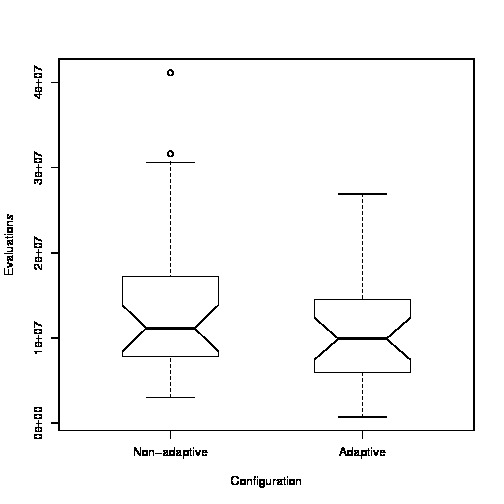
\includegraphics[width=10cm]{gfx/osgiliath/datos.jpg}
\caption{Boxplot of the number of evaluations in each configuration.}
\label{fig:osgiliath:boxplot}
\end{SCfigure}

\begin{SCtable}[][t]
\resizebox{9cm}{!}{
               \begin{tabular}{lll}
\hline

\rowcolor{colorCorporativoSuave}      & Non-adaptive & Adaptive \\ \hline \hline
\rowcolor{colorCorporativoMasSuave}Generations & 219403,10 $\pm$ 141692,16     & 167166,66 $\pm$ 93594,37 \\ \hline
\rowcolor{colorCorporativoSuave}Evaluations & 14041926,40 $\pm$ 9068298,82  & 10698794,66 $\pm$ 5990039,68 \\ \hline
\rowcolor{colorCorporativoMasSuave}Time    & 68766,40 $\pm$ 45073,04     & 51710,40 $\pm$ 29329,21 \\ \hline 
\end{tabular}
    }    
\caption{Results obtained using the Asynchronous Enabler.}
\label{tab:osgiliath:resultsenabler}
\end{SCtable}



Table \ref{tab:osgiliath:resultsenabler} shows the results obtained of the 30 executions of the two configurations tested. As it can be seen, automatic and adaptive enabling of selection operators has allowed an increase of performance, reducing time and evaluations (both significantly with a p-value$<$0.05 of a Wilcoxon test). It must be remarked that the aim of this work is not the numerical results obtained. This example has been used to demonstrate that applying a methodology to develop loose coupled services that can be dynamically bound, without modification of the existing services, can be used to achieve better results.




\subsection{Comparing with other Frameworks}
Since the OSGi framework adds features to the implementation of the
algorithm that are similar (and even superior) to those offered by
several of the frameworks described in Chapter
\ref{chap:distributedEAs}, the same algorithm (with the same operators
and parameters) has been coded using several well known frameworks, % ¿Estás comparando tu framework con el resto? Pero esto no tiene que ver con OSGi, sino con la implementación en sí. - JJ % Agh. Además, ¡¡diferentes lenguajes de programación!! - JJ FERGU: afu, fue lo que me dijeron los reviewers del paper de la SoCo, si quieres lo quito
Table \ref{tab:times} shows the execution time achieved, average
such as Mallba (C++), Algorithm::Evolutionary (Perl), and ECJ
(Java). 
solution, and Lines of Code (LoC) needed to integrate the algorithm
for each framework. All the algorithm implementations have been
executed on the same computer, an Ubuntu 12.04 Linux machine with
Intel Core2 Quad CPU Q8200 @ 2.33GHz, 4 GB RAM, without any
distribution mechanisms. The LoC have been calculated using {\em
  sloccount} program. 






\begin{SCtable}[][t]
\resizebox{11cm}{!}{
\begin{tabular}{llll}
\hline
\rowcolor{colorCorporativoSuave}Name    &  Average solution    & Average Time (s)  & LoC \\
\hline\hline
\rowcolor{colorCorporativoMasSuave}OSGiLiath               &   612.36 $\pm$ 6.05  & 0.19 $\pm$ 18.21 &  10\\
\rowcolor{colorCorporativoSuave}OSGiLiath (without OSGi)&   613.36  $\pm$ 4.50 & 0.19 $\pm$ 22.74 &  103\\
\rowcolor{colorCorporativoMasSuave}MALLBA                  &   578.76 $\pm$ 7.48  & 0.16 $\pm$ 0.0003 &  2073\\
\rowcolor{colorCorporativoSuave}ECJ                     &   602.76 $\pm$ 6.08   & 1.40 $\pm$ 0.03 &  5\\
\rowcolor{colorCorporativoMasSuave}Algorithm::Evolutionary &   617.60 $\pm$ 12.92  & 7.78 $\pm$ 0.29 &  41\\
% venga ya, 41 líneas Algorithm::Evolutionary... - JJ Fergu: Yo que se, me dio Pedro un .pl que hizo él y se lo pasé a ese
\hline
\end{tabular}
}
\caption{Comparison of tested EA frameworks in time and development.}
\label{tab:times}
\end{SCtable}

Results show that time of services of OSGiLiath is not affected by the
OSGi framework: times are almost identical to the integration with
Java code. Note that, although are services developed under SOA, and
bound in runtime, they are not distributed. Algorithmically, all
frameworks behaves the same, and results are not quite different. The
differences among frameworks are produced because the different
implementations of random generators, operators or logs, for
example. In the work of \person{Merelo \etal} \cite{PERL}, these
different behaviours are also justified. % Aquí estás comparando miles
                                % de cosas: lenguaje, máquina virtual
                                % de la misma, implementación del
                                % algoritmo, de los operadores,
                                % representación, miles de
                                % cosas. Además, es sólo 1
                                % comparación. Para ser justo,
                                % deberías comparar tamaños diferentes
                                % de cromosoma, tamaños diferentes de
                                % población y diferentes
                                % parametrizaciones. En todo caso, en
                                % una tesis con un sólo experimento no
                                % vas a ningún lado - JJ 



Regarding LoCs, MALLBA has the higher number: this is because every
% Tienes que mostrar el código y acceso a los resultados
% "crudos". Estas comparaciones de tiempo siempre son complicadas. En
% todo caso, querría ver el de A::E - JJ
algorithm is created as a ``skeleton'' and a duplication of code exist
for each algorithm and problem to execute. This is produced because
many operations affect global variables: for example the method {\em
  select\_offsprings()} affects the global variables {\em parents} or
{\em aux}. Using this method as an external service would require a
whole change in many parts of the code. Thanks the loose-coupling of
Perl, many lines of code are saved using Algorithm::Evolutionary,
mainly because many parameters and operators are defined by default. 



ECJ and OSGiLiath do not require code to combine different operators,
only to modify configuration files without re-compilation. % ¿Estas
                                % líneas las has incluido? - JJ
The difference is in ECJ the available operators must be known prior
to execution (the interfaces are linked in the source code), while in
OSGiLiath, all interfaces are bound in configuration files, or even
without them (for example, appearing in the same network/machine). But
there also exist limitations, because ECJ only provides a fixed ways
of distribution mechanisms, and only certain parts of the framework
can be accessed remotely, while in OSGiLiath all operators have the
chance to be distributed if desired, modifying the configuration
files. 


It must be remarked that OSGiLiath does not try to compete with the
other frameworks (they are widely accepted, completed and tested), it
is only an example of how to develop EAs under the SOA paradigm. % ¿Esta es la conclusión? ¿Del capítulo? FERGU: añadida sección conclusiones

\subsection{Increasing interoperability with other systems}

As previously stated, another advantage of SOA is the programming
language independence respect to the service interfaces. Although OSGi
is a kind of SOA, it does not include  the capability of
interoperability with other kind of services by default. However,
adaptation services can be added to transform OSGi interfaces into
other SOA interfaces, such as Web Services (presented in Chapter
\ref{chap:soa}). So, services that are not written in Java, neither
OSGi-based, could use services implemented in OSGiLiath (and
vice-versa). 



For example, using ECF all OSGi service interfaces are
transformed into WSDL  interfaces (explained in Section \ref{subsec:soa:ws}) automatically. % ¿Qué es wsdl? ¿Por
                                % qué es importante? ¿Lo usas? Si no,
                                % ¿por qué diablos lo dices?  JJ FERGU: referenciado, y lo uso
Thus, these services could be used from other systems, that do not
need to know the implementation language of the services in
OSGiLiath. An example where an OSGi interface is transformed into a
WSDL interface is shown in Figure \ref{AXISFIGURE}. % ¿Es tuya? ¿Por
                                % qué la pones en la tesis? - JJ FERGU: claro que es mía. La pongo porque la uso.
The computation
node A, based on OSGi, uses the OSGi interface of the computation node
C to calculate the fitness. Node B uses the WSDL interface to do the
same task. It is not necessary to modify existing services source code
to convert an OSGi interface into a WSDL interface. This
transformation is bi-directional: given an WSDL interface, it can also
be transformed into a service to use inside OSGi. For example, the
algorithms in GridUFO framework (presented in Chapter
\ref{chap:distributedEAs}) could be used from OSGiLiath. % Cada vez
                                % que dices "could be" y no "will be
                                % used and presented in Chapter A"
                                % $deity mata a un cachorro de especie
                                % en peligro de extinción de pelo
                                % sodoso y grandes ojos. - JJ






\begin{SCfigure}[20][htb]
\centering
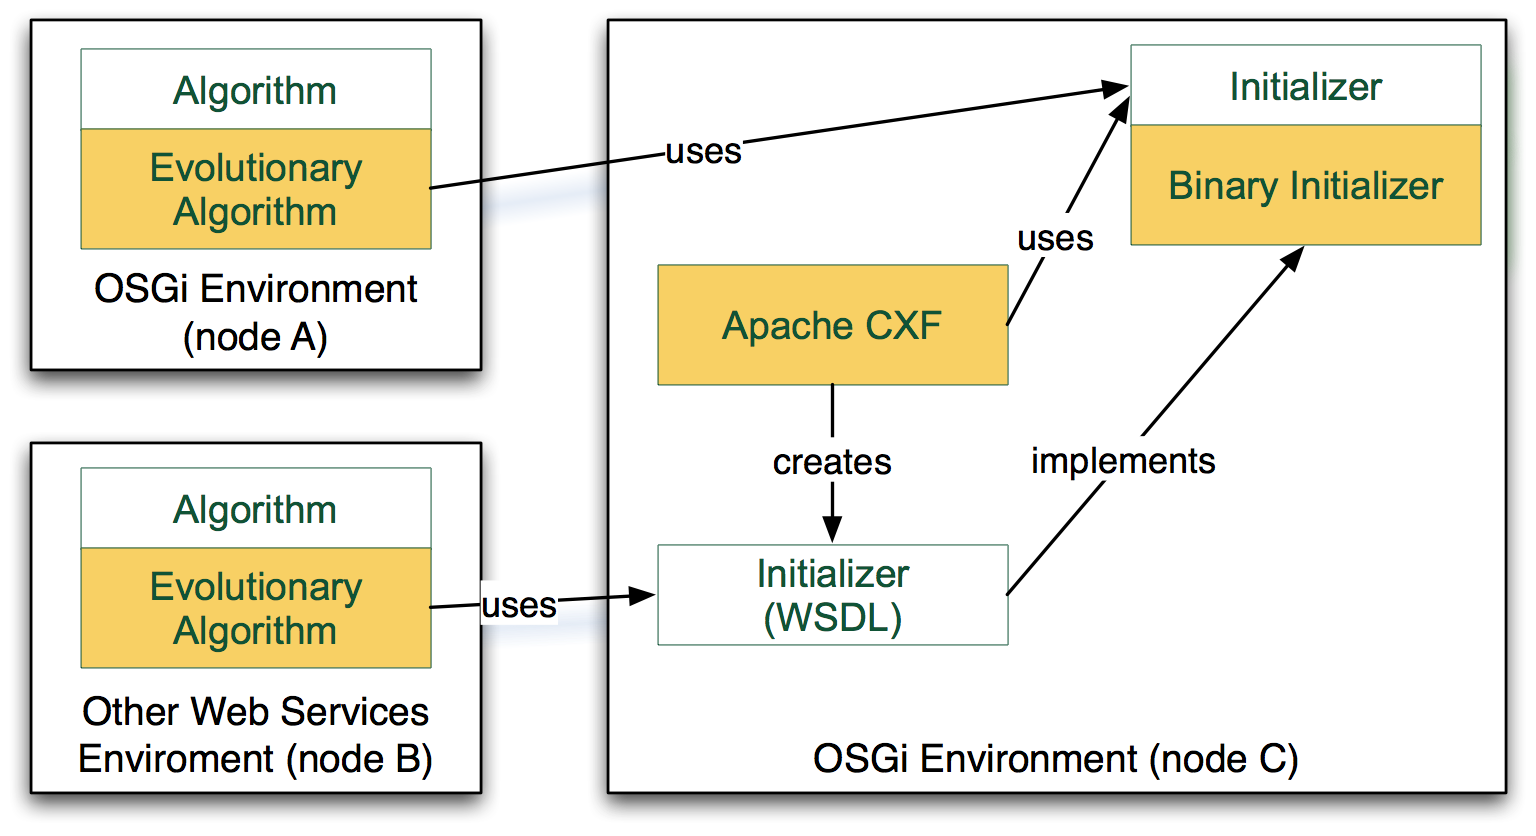
\includegraphics[width=10cm]{gfx/osgiliath/axis.png}


\caption{Communication with other kind of services. ECF service automatically creates WSDL interfaces for the OSGi interfaces to be used from other environments}
\label{AXISFIGURE}
\end{SCfigure}

\section{Conclusions}
% Tienes que alcanzar alguna conclusión fuerte: la implementación
% refleja el modelo y lo valida. ¿Es el modelo válido? ¿Cómo lo has
% probado? ¿Es la implementación válida? ¿Cómo lo has probado? - JJ FERGU: Escritas las conclusiones, que antes no había

In this chapter, the steps of implementation and deployment of services have been used to create a framework that...

The source code of OSGiLiath is available in \url{http://www.osgiliath.org} under a GNU/LGPL license.
}{\myChapter{Implementation of SOA-EA}\label{chap:osgiliath}}
\ifthenelse{\equal{\value{IncluyeCapitulo}}{2}}{\myChapter{Parameter adaptation in heterogeneous machines}\label{chap:adaptive}



\begin{flushright}{\slshape
    It's a wonderful thing, as a writer, to be 
    \\given parameters and walls and barriers.} \\ \medskip
    --- {Neil Gaiman}
\end{flushright}

\minitoc\mtcskip
\vfill
\lettrine{T}{he} last objective of this thesis is to apply the created framework to solve the problems previously addressed, and therefore, to be used to perform some kind of research. In this chapter, the capabilities of OSGiLiath will be used to investigate if adapting the parameters of a distributed EA taking into account the computational capabilities of the different nodes of execution leads to an increase of performance.
%FERGU: añadido el párrafo de arriba para enlazar con la tesis
% UN OBJETIVO DE LA TESIS NO PUEDE SER "HACER INVESTIGACIÓN". ¿La
% tesis es Osgiliath? ¿Qué has usado de un algoritmo genético basado
% en SOA que no podrías haber hecho con otro algoritmo? 

% Planteamiento incorrecto y, como en las conclusiones, estoy tentado
% de borrarlo todo. El enfoque debe ser
% "Parte de la adaptación de un algoritmo evolutivo a una arqutiectura
% heterogénea y dinámica es tener en cuenta y aprovechar las
% diferentes capacidades de los nodos que se vayan añadiendo a la
% red. Estos nodos pueden tener diferentes capacidades, etc,
% etc... por eso, como parte de la metodología que implementa AGs
% sobre tal, en este capítulo examinamos posibles estrategias de
% adaptación pare evaluar cuál es la más adecuada paraellas". Si no te
% gusta esto, pregúntate siempre cuál es TU TESIS y en qué contribuye
% este capítulo a probarla - JJ 
This question is interesting due to new trends in distributed computing presented in Chapter \ref{chap:soa}, such as Cloud Computing, GRID
 or Service Oriented Science
 are % si se han presentado en los capítulos
                             % previos, tendrás que hacer referencia a
                             % los mismos - JJ FERGU: hecho.
leading to heterogeneous computational devices, including for instance, laptops,
tablets or desktop PCs, working in the same
environment. Thus, many laboratories, which do not count with classic
clusters but the usual workstations used by scientists, can leverage
this motley set as a heterogeneous cluster. As explained in Chapter \ref{chap:distributedEAs}, Distributed Evolutionary
Algorithms have been tested successfully in this type of systems and they have 
become very popular because their implementation is
not complex \cite{AsynchronousMultidemeMerelo08}. % Cita del asynchronous EAs del PPSN de Dortmund - JJ FERGU: hecho
Also, as presented in Chapter \ref{chap:soa}, a possible way to increase 
the interoperability within these systems is SOA, and specifically, the use of OSGiLiath framework as an example.


% frase guay, pero tienes
                                % que enganchar todo esto con LA TESIS
                                % - JJ FERGU: Hecho




%In previous chapter OSGiLiath was proposed as a framework to solve determined issues in the EA development, using a specific SOA technology. 

In this chapter, OSGiliath will be used % ¿Se podía haber usado otra
                                % cosa? ¿Esto es exclusivo de
                                % Osgiliath? - JJ FERGU: Frase al principio del capitulo
 to create a heterogeneous distributed system to be used to develop a scientific research related with parameter tuning and control (explained in Section \ref{chap:distributed:pcontroltuning}). Several services to deal with automatic binding and parameter control will be developed following SOA-EA, and deployed in different cluster configurations.






%In Section \ref{}, % where? - JJ FERGU: hecho
% we presented the work of \person{Alba \etal}, where dEAs with the same parameter
% configuration are even % cita el capítulo, no el trabajo!!! - JJ 
%more efficient in time and evaluations on heterogeneous hardware configurations than on clusters with
%homogeneous devices. % ¿en qué condiciones? ¿Siempre? Así, en general, no puede ser cierto. Un cluster de Xeons no va a ser más rápido que un Xeon y dos i5s - JJ 
%This can be explained by different reasons, such
%as different memory access times, cache sizes, or even
%implementation % ¿son más rápidos porque los tiempos de acceso a
               % memoria son diferentes? Hay que ser preciso, no vago
               % Además, ¿por qué cuentas eso? ¿Si ya se sabe, para
               % qué quieres repetirlo? ¿Estás confirmando un
               % resultado? ¿Mejorándolo? - JJ
%languages or compilers in each machine, leading to a different
%exploitation/exploration rate of the search space.  % ¿Una tasa
                                % diferentes de
                                % exploración/explotación es buena?
                                % ¿Por qué? ¡Mira mi artículo del PPSN
                                % en 2008! - JJ
%Heterogeneous parameter configuration  has also been shown to be more  efficient time-wise than a fixed
%set of parameters for different problems, as shown by \person{Gong and Fukunaga} \cite{Gong2011HeterogeneousParameters}.   


%FERGU: Comentado todo esto y arreglado párrafo arriba para justificarlo con la tesis
%These facts have motivated us to study a combination of both ideas: % esos hechos no pueden haberte motivado a estudiar nada. Tiene que haberlo hecho LA TESIS. ¿Qué tiene que ver con todo esto? - JJ
%dEAs on a heterogeneous set of nodes with different parameter values
%adapted to each node. % ¿Por qué? ¿Porque es nuevo, y por tanto mejor?
                      % ¿Porque es diferente y por tanto publicable? ¿Qué te dice que vaya a
                      % ser mejor? Y, lo más importante, ¿cómo
                      % contribuye a LA TESIS? - JJ
%In this study, the parameter to adapt to the
%computational power of each node has been the sub-population size of
%each island. % ¿Por qué? ¿Cómo? ¿Cómo se relaciona esto con LA TESIS?
             % Los capítulos deben probar LA TESIS, no decir qué se ha
             % hecho como un hecho consumado. - JJ FERGU: BORRADO TODO Y PUESTO A CONTINUACIÓN

\section{Background and problem definition}
In Section \ref{subsec:distributed:adapthetero} several works about adaptation in heterogeneous environment were presented. For example, the work of \person{Alba \etal}, where dEAs with the same parameter configuration could be more efficient in time and evaluations on heterogeneous hardware configurations than on clusters with homogeneous devices, or the work of \person{Gong and Fukunaga}, where different parameters in each island increased performance.

 These trends have motivated the usage of OSGiLiath in this chapter to give an insight to the following research questions:
\begin{itemize}
 \item Can a distributed EA be adapted to leverage the capability of a
   heterogeneous cluster?  % ¿Esa son las preguntas de la TESIS?
                           % ¿Dónde lo has dicho? - JJ FERGU: son preguntas DEL CAPÍTULO (puesto)
 \item How the adaptation of the sub-population size to the
   computational power affects the execution time and number of
   evaluations?  % Y esta pregunta es interesante porque... - JJ
 \item Is there any difference between using the same sub-population sizes in a homogeneous and a heterogeneous cluster?
 \item How is each service of the algorithm (selection, recombination, mutation, replacement and migration) affected by the different
   configurations?  % ¿Y cómo afecta todo esto a LA TESIS? - JJ
\end{itemize}

The aim of this chapter is to use OSGiLiath to demonstrate if adapting the sub-population size to the computational power of an heterogeneous cluster nodes presents an improvement in execution time. New services will be created to deal with different distributed nodes and setting the population sizes.




\subsection{Algorithm to develop}

The experimentation is centred in a distributed GA. Figure \ref{fig:EAused} shows the pseudo-code of the used algorithm. 
The algorithm is steady-state, i.e. every generation the offspring is
mixed with the parents and the worst individuals are removed. This algorithm is general enough and not designed specifically for this study.

% 1: los
                                % detalles de los EAs tendrías que
                                % haberlos dichos en su capítulo. 2:
                                % ¿Por qué SS? ¿Si no lo fuera, sería
                                % cierto? - JJ FERGU: añadida arriba
 The used neighbourhood topology for migration between islands (nodes)
 is a ring (see Figure \ref{fig:ring} in Chapter
 \ref{chap:distributedEAs}). The best individual is sent to the
 neighbour in the ring, after a fixed number of generations in each
 island. The algorithm stops when the optimum (the solution to the
 problem) is found.   % ¿Pogqué? ¿Pogqué? No puedes soltar un montón
                      % de decisiones de sopetón sin justificarlas (y
                      % sin relacionarlas con LA TESIS) - JJ FERGU: enlazado con la tesis a continuación
Therefore, a mechanism to stop all the executing nodes must be implemented.

\newsavebox{\algoadaptativebox}
\begin{lrbox}{\algoadaptativebox}
\begin{minipage}{10cm}
\begin{algorithmic} %Esto podías haberlo usado también en otros
                    %capítulos - JJ FERGU: En el unico sitio donde no lo he usado es en el del BasicGA de Eiben.
\STATE population $\gets$ initializePopulation()
\WHILE {$stop criterion not met$}
    \STATE parents $\gets$ selection(population)
    \STATE offspring $\gets$ recombination(parents)
    \STATE offspring $\gets$ mutation(offspring)
    \STATE population $\gets$ population + offspring
    \IF {time to migrate}
      \STATE migrants $\gets$ selectMigrants(population)
      \STATE remoteBuffer.send(migrants) % si haces esto, hazlo
                                % bien. ¿Dónde se declaran las
                                % variables? - JJ
    \ENDIF
    \IF {localBuffer.size $\neq$ zero}
      \STATE population $\gets$ population + localBuffer.read()
    \ENDIF
    \STATE population $\gets$ removeWorst(population)
\ENDWHILE
\end{algorithmic}
\end{minipage}
\end{lrbox}

\begin{SCfigure}[20][tb]
\usebox{\algoadaptativebox}
\caption{Pseudo-code of the used dEA: a distributed Genetic Algorithm
  (dGA).} % ¿Esto es tuyo? ¿Genérico? Si es genérico a) debería ir a
          % su capítulo b) deberías citar dónde se ha publicado - JJ
\label{fig:EAused}
\end{SCfigure}




\subsection{Problems to solve}
%No empieces con "the problems to evaluate". Di que los resultados
%deberían ser más o menos independientes del problema, pero se han
%elegido estos por tal y cual. Tienes que justificar que con estos es
%suficientes, para que no te digan el clásico "Prueba otro algoritmo"
%- JJ

The results should be independent of the problem used, but the next ones have been selected because they cover different characteristics
and computational demands. %coñe, no lo digas
                           %literlamente. ¡Justifícalo todo! ¿Qué
                           %características cubren? ¿Qué demandas
                           %computacionales? - JJ
 The problems to evaluate are the Massively Multimodal Deceptive
Problem (MMDP)  and the OneMax problem. Both problems have been described previously in Section \ref{sec:osgiliath:experiments}. Each one requires different actions/abilities by the GA
at the level of population sizing, individual selection and
building-blocks mixing \cite{AsynchronousMultidemeMerelo08}. % Podías citar los trabajos de Juanlu en esto
                        % y/o Lobo y/o Carlos Fernandes - JJ FERGU: pongo este




\subsection{Hardware and parameter configurations}

% Hala, un itemize a pelo, sin jugueteo previo ni ná de ná... ¿Por qué
% estas cuatro configuraciones? ¿Qué dificultad a priori tienen? - JJ FERGU: puesto abajo

As we are going to test parameter adaptation to hardware, different configurations should be used to compare and validate if the change in the parameters depends only of the parameters, the hardware heterogeneity, or the combination of both.

\begin{itemize}
\item HoSi/HeHa: Homogeneous Size/Heterogeneous Hardware. The same sub-population size in each island on a heterogeneous cluster.
\item HeSi/HeHa: Heterogeneous Size/Heterogeneous Hardware. Different
  sub-population sizes in each island on a heterogeneous cluster. % ¿different como? - JJ
\item HoSi/HoHa: Homogeneous Size/Homogeneous Hardware. The same
  sub-population size in each island on a homogeneous cluster. % hardware y software, ¿no? Deberías decir algo como "system" - JJ FERGU: ya, pero system puede ser también software. Prefiero dejarlo así para que quede claro todo
\item HeSi/HoHa: Heterogeneous Size/Homogeneous Hardware. Different sub-population sizes (the obtained for HeSi/HeHa) in each island on a homogeneous cluster.

\item AdSi/HeHa: Adaptive Size/Heterogeneous Hardware. Online adaptation of sub-population sizes in each island on a heterogeneous cluster.
\end{itemize} % ¿No falta AdSi HoHa? ¿Por qué no lo has puesto? - JJ FERGU: porque como la velocidad es la misma no hay cambios. Pero sí, lo pongo.



\subsection{Homogeneous Size configuration}

In this configuration, each node has 256 individuals (so, the total
amount is 1024).  % ¿Por qué? - JJ

The results of executing the algorithm in the will be used to set the sizes of the next configuration.




% ¿Ya está? ¿Nada de laxitud pos-tabla? Ahí está, y apáñatelas, ¿no? - JJ


\subsection{Heterogeneous Size configuration}

Our aim consists in validating the following hypothesis: adapting the %%%%QUITAR ESTO QUE LO HE PUESTO ARRIBA IGUAL!!!
sub-population size to the computational power of the heterogeneous
cluster nodes presents an improvement in execution time. % Hombre, ya
                                % era hora de que supiéramos la
                                % hipótesis. ¿No queríamos responder a
                                % unas preguntas? ¿Qué ha pasado con
                                % eso? ¿Cómo engancha eso con LA
                                % TESIS? - JJ
In this chapter, for a possible offline way to calculate the computational performance of each node, % ein? - JJ fERGU
 the average number of generations obtained in the
HoSi/HeHa configuration for both problems will be used to determine the
computational power of the heterogeneous machines. This comparison
takes into account all the evolutionary process in a fair manner
(proportional to the memory, processor and network usage), instead of a
traditional benchmark that usually relies only on the CPU
speed. %Hay benchmarks de todo tipo. No se puede hablar de benchmarks
       %"tradicionales" a no ser que tengas pruebas de dónde se
       %utilizan y lo cites - JJ
 %Although this is not obviously the best way, %¿Cuál es la mejor
                                %manera? ¿Por qué no la usas? - JJ FERGU: comentado
 %it is a possible
The proposed technique is a possible way to establish the computational power for the experiments of this
chapter and to determine if changing the sub-population size according
the computational power reduces the computing time of the whole
approach. %It should be considered that the contribution of this chapter
%is not the way we have computed these sizes, but compare the algorithm
%with parameters adapted to their power. % está mal escrito y aunque
                                % estuviera bien no se entiende y/o
                                % suena a excusa - JJ FERGU: lo quito, tampoco dice nada

Thus, we have used the obtained average number of generations in the
previous sub-section (Table \ref{table:generations}) to set
proportionally the sizes in the HeSi/HeHa and HeSi/HoHa
configurations, by dividing the total number of individuals
(1024). Note that, even having two nodes with the same processors and
memory (HeN1 and HeN2), they could have different computational power:
this may be produced by different operating systems, virtual machine
versions, or number of processes being executed (inside a node). % ¿Y
                                % qué conclusiones sacas? ¿Estás
                                % probando la hipótesis? ¿No? - JJ



\subsection{Adaptive Size configuration}

%Finally, in order to validate the hypothesis that adapting the
%sub-population sizes to computational resources of a heterogeneous
%cluster leads to an improvement of the time needed to obtain the
%solution,  % el inglés de este capítulo es desastroso. Por favor,
           % revisalo bien - JJ FERGU: reescrito abajo
A third experiment is proposed to validate the hypothesis of sub-population 
size adaptation to computational resources. In this case, the adaptation
of the sub-population size to the computational power of the islands
(nodes) is performed during runtime (online). % tienes que cualificar
                                % la hipótesis, porque la situación es
                                % diferente. O precisar qué significa
                                % adaptación; si auto-adaptación o
                                % cambios de parámetros. - JJ
  Each time a node ($N$) receives an individual, it compares its
  current number of generations ($Gen_{N}$) with the ones of the node
  who sent the individual (node $N-1$ in the ring). Then, the
  sub-population size is adapted proportionally to the difference in
  the number of generations, following the next equation: % ¿todo esto
                                % te lo has sacado de la manga? ¿Qué
                                % quieres hacer? ¿Cómo has llegado a
                                % esta conclusión? No cuentes nunca en
                                % una tesis lo que has hecho, cuenta
                                % el proceso por el que has llegado a
                                % esa conclusión - JJ

\begin{equation}
size'_{N}=\dfrac{Gen_{N}}{Gen_{N-1}}size_{N}
\end{equation}

If the new size is larger than the actual size, new individuals are
added to the sub-population cloning random existent ones. % ¿Por qué?
                                % No lo escribas todo como si pasaras
                                % por aquí, ¡es una tesis! - JJ
Otherwise, the sub-population must be reduced and thus, the worst are removed. Therefore, the service {\em Population} is used to manage the population, as explained in Chapter \ref{chap:osgiliath}.

With this possible online adaptation scheme, each node only requires
to receive information from one of the neighbours and not from the
whole system. % ¿Por qué? - JJ
Thus, each node tends to have a number of individuals proportional to
their computational power with respect to the other nodes. Experiments
on homogeneous cluster do not alter the sub-population sizes, since
the number of current generations are equal in all nodes during
runtime. % cuidado con el inglés, dos correcciones aquí - JJ

\subsection{Restrictions}
Once the problem to solve, the algorithm to implement and the different configuration have been described, the restriction to the services to develop are the summarized:
\begin{itemize}
\item There is not a central control node.
\item The number of nodes participating in the experiment should not be fixed.
\item All nodes automatically bind the available distribution (migration) services.
\item The nodes must stop when the optimum is found.
\item Services must be executed in heterogeneous machines with different operating systems and architectures.
\item It is necessary a log service to show the current state of the algorithm and service timings.
\end{itemize}


\section{Designing the services with SOA-EA}
Once the description of the system to develop has been presented, the SOA-EA methodology (explained in Chapter \ref{chap:soaea}) is used to create a SOEA that fulfils the previous requirements.

\subsection{Identification}

In addition of the services for calculating the fitness of the problems ({\em MMDPFitnessCalculator} and {\em OneMaxFitnessCalculator}), or the {\em OptimumStopCriterion} and crossovers and mutators created in previous chapter, new services should be added. The first one deals with the migration between islands, so, a service {\em Migrator} (to receive and send individuals from/to other nodes) needs to be created. Also, it is necessary a service to start or stop the remote loops in all islands at the same time (service {\em Launcher}). Finally, it is necessary a to manage the received individuals from the migrators and control the population size, this can be performed in a new {\em Replacer} interface: {\em AdaptiveReplacer}.

\subsection{Specification}

The service {\em Launcher} and its specification {\em ExperimentLauncher} automatically binds all available {\em Algorithm} services in the network. This service can start all the distributed EAs at the same time (for example, from command line when all nodes are online and they services bound). When one of the EAs has finished, it has to notify the others to stop. 

To perform the migration taking into account the previous requirements, each node offers a migration buffer to
accept foreign individuals. Also, in order to reduce bottlenecks in
distributed executions, asynchronous communication needs to  be provided
to avoid idle time using reception buffers (that is, the algorithm
does not wait until new individuals arrive, but the buffers cannot be
used again until the reception is done). This kind of communication
offers an excellent performance when working with different nodes and
operating systems, as demonstrated in \cite{AsynchronousMerelo08}.

The {\em Migrator}  has two operations: {\em send} and {\em read}. The first one is used to send the individuals to the migrator, and the other is used to read the individuals of that migrator. Usually, each node (island) has one migrator to receive individuals, and references to the other nodes' migrators. In our case, the implementation of {\em Replacer} binds the local {\em Migrator} to write in it the individual(s) to sent. In this chapter, the {\em Migrator} implementation is the {\em MigratorRingBuffer}: this class implements that interface and automatically binds all the Migrators available in the environment (in a vector of references). So, the migrators can be added during runtime, and no stop the algorithm if one node fails.  The {\em MigratorRingBuffer} sends the individuals to the remote Migrator whose id is inmediatelly higher than the local id (or the smaller, if it not exist) following a ring topology. Figure \ref{MIGRATOR} shows this configuration. The {\em Replacer} implementation, a reference to the local {\em Migrator} interface just send and read the individuals. The {\em MigratorRingBuffer} implementation binds an unbinds other migrators in other nodes, keeping a reference to these remote service interfaces. The {\em AdaptiveReplacer} implementation binds the local {\em Migrator} service and it manages the population sizes.




\begin{SCfigure}[20][tb]
\centering
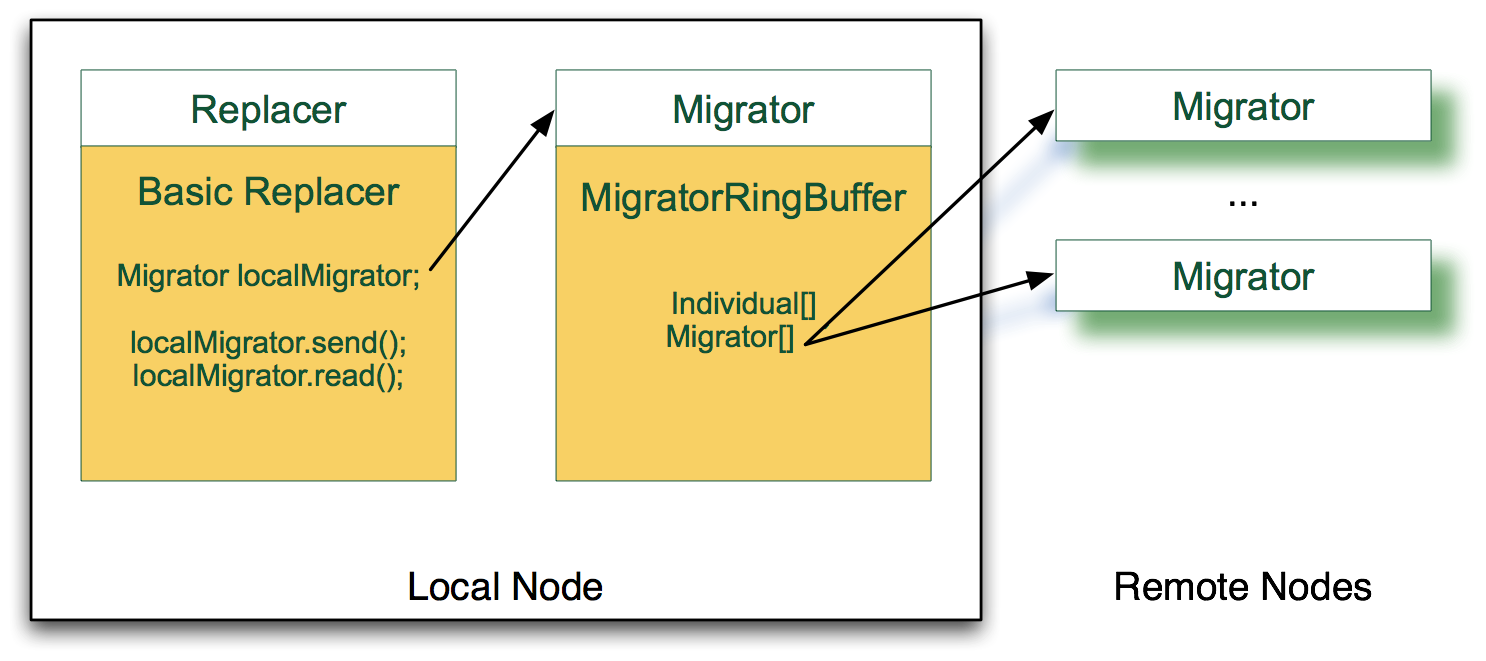
\includegraphics[width=10cm]{gfx/osgiliath/migrator.png}


\caption{Using the Migrator service to create a distributed island EA with a ring topology (white boxes are service interfaces and orange boxes are implementations).}
\label{MIGRATOR}
\end{SCfigure}

% Cada algoritmo debe ser como un paper. No te puedes ir a
% Experimental results para saber qué diablos quieres probar y cómo
% quieres hacerlo. Además, tienes que introducir el resto del capítulo
% y exponer la línea argumental del mismo y como contribuye a la
% tesis. Perdón, LA TESIS - JJ FERGU: teniendo en cuenta todo esto, como estarás viendo

\subsection{Implementation and Deployment}

All services have been implemented in OSGiLiath. The {\em Migrator} and {\em Algorithm} services are exposed using ECF Generic Server, as explained in Section \ref{sec:osgiliath:technology}). This services are, therefore, automatically bound to each node in the clusters, without notify their IP address. Extra code to manage the communication has not been added, as all services are undistinguishable of being remote or local. Remote {\em Migrators} and {\em Algorithms} are bound thanks to the bind/unbind methods of declarative services and ECF (explained in Section \ref{sec:osgiliath:technology}). Several properties can added to the service allows to ECF automatically announce the implementation to all nodes in the network and no specific code is required to change from one distribution mechanism to another.

The services have been deployed in two different computational systems: a {\em
  heterogeneous cluster} % no es un cluster, simplemente un grupillo
                         % de ordenadores - JJ
and a {\em homogeneous cluster}. The first
one is formed by four different computers of our lab with different
processors, operating systems and memory size. The latter is a
dedicated scientific cluster formed by homogeneous nodes. Table
\ref{tabcomputers} shows the features of each system and the name of
the nodes. % El espacio HeHa es muy amplio. Podrías haber probado
           % diferentes configuraciones de este: más diferencia, menos
           % diferencia... de hecho, deberías hacerlo para esta tesis
           % (y trabajos posteriores) - JJ

\begin{SCtable}[][t]
\resizebox{11cm}{!}{
\begin{tabular}{|c|c|c|c|c|}
\hline
\rowcolor{colorCorporativoSuave}Name     & Processor  & Memory  & Operating System  & Network  \\ \hline \hline
\multicolumn{5}{|>{\columncolor{colorCorporativoMasSuave}}c|}{Homogeneous cluster} \\ \hline
\rowcolor{colorCorporativoSuave}HoN[1-4] &  Intel(R) Xeon(R) CPU   E5320  @ 1.86GHz       & 4GB & CentOS 6.7    &   Gigabit Ethernet    \\ \hline
\hline
\multicolumn{5}{|>{\columncolor{colorCorporativoMasSuave}}c|}{Heterogeneous cluster} \\ \hline
\rowcolor{colorCorporativoSuave}HeN1  &  Intel(R) Core(TM)2 Quad CPU    Q6600  @ 2.40GHz    & 4GB   & Ubuntu 11.10 (64 bits)  & Gigabit Ethernet      \\ \hline
\rowcolor{colorCorporativoMasSuave}HeN2  &  Intel(R) Core(TM)2 Quad CPU    Q6600  @ 2.40GHz    & 4GB   & Ubuntu 11.04 (64 bits)  & Gigabit Ethernet      \\ \hline
\rowcolor{colorCorporativoSuave}HeN3  &  AMD Phenom(tm) 9950 Quad-Core Processor @ 1.30Ghz    & 3GB   & Ubuntu 10.10 (32 bits)  & 100MB Ethernet      \\ \hline
\rowcolor{colorCorporativoMasSuave}HeN4  &  Intel (R) Pentium 3 @ 800MHz               & 768 MB  & Ubuntu 10.10 (32 bits)  &   10MB Ethernet     \\ \hline
\end{tabular}
\caption{Details of the clusters used: a homogeneous cluster (Ho), and a heterogeneous cluster (He)}
\label{tabcomputers}
}
\end{SCtable}

\section{Experimental results}

Once the services have been created, the different combinations of systems and parameter are evaluated. Table \ref{table:parameters} summarizes all the parameters used in the
experiments. % ¿Explicación? ¿Has probado otros?  - JJ




                                \begin{SCtable}[][t]{
\begin{tabular}{ccccc} \hline
\rowcolor{colorCorporativoSuave}Node        & HeN1     & HeN2      & HeN3     & HeN4   \\ \hline \hline
\multicolumn{5}{>{\columncolor{colorCorporativoMasSuave}}c}{MMDP problem} \\ \hline
\rowcolor{colorCorporativoSuave}Generations & 10990.25 & 10732.075 &  7721.15 & 717.95 \\ \hline
\rowcolor{colorCorporativoMasSuave}Proportion  & 36.43    & 35.58    & 25.59    & 2.38    \\ \hline
\multicolumn{5}{>{\columncolor{colorCorporativoSuave}}c}{OneMax problem} \\ \hline
\rowcolor{colorCorporativoMasSuave}Generations & 2430.27 & 2353.77 & 1423.77 & 91.5 \\ \hline
\rowcolor{colorCorporativoSuave}Proportion  & 38.58   & 37.36   & 22.6   & 1.45 \\ \hline
\end{tabular}
\caption{Average number of generations in each node needed to find the
  optimum on the heterogeneous cluster with heterogeneous size.}
\label{table:generations}
}
\end{SCtable}











\begin{SCtable}[][t]
\resizebox{11cm}{!}{
\begin{tabular}{cc}
\hline
\rowcolor{colorCorporativoSuave}Name & Value\\ \hline \hline
\rowcolor{colorCorporativoMasSuave}Crossover type & Two-point crossover \\ \hline
\rowcolor{colorCorporativoSuave}Crossover rate & 0.5\\ \hline % muy
                                % bajo probablemente.
\rowcolor{colorCorporativoMasSuave}Mutation probability of each gene & 1/individual size\\
\hline % esa no es una tasa de mutación, es determinista. ¿Todos
       % mutan? - JJ FERGU: arreglado
\rowcolor{colorCorporativoSuave}Selection & 2-tournament \\ \hline
\rowcolor{colorCorporativoMasSuave}Replacement & Steady-state\\ \hline
\rowcolor{colorCorporativoSuave}Generations to migrate & 64 \\ \hline
\rowcolor{colorCorporativoMasSuave}Number of individuals to migrate & 1 \\ \hline
\rowcolor{colorCorporativoSuave}Stop criterion & Optimum found \\ \hline
\rowcolor{colorCorporativoMasSuave}Individual size for MMDP & 150 \\ \hline
\rowcolor{colorCorporativoSuave}Individual size for OneMax & 5000 \\ \hline
\rowcolor{colorCorporativoMasSuave}Runs per configuration & 40 \\ \hline
\hline
\rowcolor{colorCorporativoSuave}Total individuals in HoSi and HeSi & 1024\\ \hline \hline
\rowcolor{colorCorporativoMasSuave}Sub-population size in each node in HoSi & 256  \\ \hline
\rowcolor{colorCorporativoSuave}Sub-population sizes in HeSi for MMDP
& 374, 364, 262 and 24 (from N1 to N4) (see Section \ref{subsec:adaptive:hesisizes})\\ \hline % ¿REsultado? ¿Cómo se
                                % ha obtenido? - JJ FERGU: añado referencia
\rowcolor{colorCorporativoMasSuave}Sub-population sizes in HeSi for OneMax & 396,  382, 232 and 14 (from N1 to N4) (see Section \ref{subsec:adaptive:hesisizes})\\ \hline
\hline
\rowcolor{colorCorporativoSuave}Maximum island size in AdSi & 1024 \\ \hline
\rowcolor{colorCorporativoMasSuave}Minimum island size in AdSi & 16 \\ \hline
\rowcolor{colorCorporativoSuave}Initial island size in AdSi & 256 \\ \hline 
\end{tabular}
}
\caption{Parameters used in all configurations.}
\label{table:parameters}
\end{SCtable}

%\section{Implementation in OSGiLiath}
%In order to deal with the operating system and architecture
%heterogeneity (different operating systems, processors, compilers,
%etc.), the OSGiLiath framework \cite{SOASOCO}, based in Java, has
%been used in this work. This is a service-oriented evolutionary
%framework that automatically configures the services to be used in a
%local network. In this case, each node offers a migration buffer to
%accept foreign individuals. Also, in order to reduce bottlenecks in
%distributed executions, asynchronous communication has been provided
%to avoid idle time using reception buffers (that is, the algorithm
%does not wait until new individuals arrive, but the buffers cannot be
%used again until the reception is done). This kind of communication
%offers an excellent performance when working with different nodes and
%operating systems, as demonstrated in
%\cite{HETEROGENEOUSHARD,AsynchronousMerelo08}. The transmission
%mechanism is based on ECF Generic server (over
%TCP)\footnote{\url{http://www.eclipse.org/ecf/}}.  The source code of
%the algorithms used in this work is available in
%\url{http://www.osgiliath.org} under a LGPL V3 License. 

% Hombre, para una cosa que nombra Osgiliath, lo quitas - JJ FERGU: añadido arriba, es que revisaste esto mu pronto! xD

The three main objectives of parallel programming are to tackle large
computational problems, increase the performance of algorithms in a
finite time, or reduce computational time to solve the problem
(reaching the optimum). In this chapter, we focus in the last
objective. % Y a los otros dos, que les den - JJ
As claimed by \person{Alba and Luque} in
\cite{Alba06evaluationParallel}, assessing the performance of a
parallel EA by the number of fitness function evaluations required to
attain a solution may be misleading. In our case, for example, the
evaluation time is different in each node of the heterogeneous
cluster, so the real algorithm speed could not be reflected
correctly. %¿Cuál es la velocidad "real"? - JJ
 However, the number of evaluations has been included in
this chapter to better understanding the results. % ¿Better que qué? - JJ
The total number of
generations carried out by all nodes, and the maximum number of
generations required by the faster node in each configuration are also
shown. It is difficult to compare the performance of HoHa and HeHa for
the same reason: the evaluation time is different in each system (and
even in each node). Thus, one of the objectives in this chapter is not
making the heterogeneous cluster comparable or better in time than the
homogeneous one (because they are, obviously, different), but showing
that the same parameter configuration can improve performance in time
on heterogeneous clusters and could not have an effect on homogeneous
ones. 
% es que, al final, estás comparando cosas que no son comparables. Si
% el cluster homogéneo es más rápido, tendrá mejores
% resultados. Tendrías que haber hecho un montaje experimental un poco
% mejor: sustituir un ordenador del cluster por uno más potente, por
% uno menos potente, dos del cluster por esos dos, luego tres, y lo
% que sea. Como parte de la tesis, deberías diseñar una metodología
% para hacer este tipo de experimentos - JJ FERGU: es que no comparo clusters entre sí, mira los boxplots como están separados. El homogéneo lo uso para ver si la mejora se debe al conjunto de parámetros o a la combinación de parámetros y hardware.

\subsection{Obtaining the HeSi sizes}
\label{subsec:adaptive:hesisizes}
After executing the algorithm 40 times per problem on the
heterogeneous cluster, % ¿Por qué? - JJ
we have obtained the average number of generations in each node, as it
can be seen in Table \ref{table:generations}. Note how the generations
attained (and their proportion in every node) to reach the optimum
depends on the problem considered (besides the hardware). % Jolines,
                                % cómo no va a depender en el problema
                                % - JJ

\subsection{MMDP results}

Table \ref{tab:resultsMMDP} shows the results for the MMDP
problem. These results are also shown in the boxplots of Figure
\ref{fig:timeMMDP} (time) and Figure \ref{fig:evalsMMDP}
(evaluations). Table \ref{tab:significanceMMDP} shows the statistical
significance of the results. First, a Kolmogorov-Smirnov test is
performed to assess the normality of the distributions. As all
distributions are not normal, we use non-parametric tests. To compare
between two methods (HoSi and HeSi in the homogeneous cluster) a
Wilcoxon test has been applied. For a three methods comparison (HoSi,
HeSi and AdSi on heterogeneous cluster) a Kruskal-Wallis test has been
used. % y esto lo haces porque... ¿Debe todo el mundo saber esto? -JJ

 In the HeHa system,  offline adaptation of  the sub-population to the computational
 power of each node makes the algorithm finish significantly earlier,
 and also, needing a lower number of evaluations to reach the solution. On the other hand, in the HoHa system,
 setting the same sub-population sizes makes no difference in time and
 evaluations, that is, changing this parameter has no influence in the
 algorithm's performance (p-value=0.52 for time and 0.08 for
 evaluations). % esto es interesante porque... - JJ


\begin{SCtable}[][t]
\resizebox{11cm}{!}{
\begin{tabular}{ccccc}
\hline
\rowcolor{colorCorporativoSuave}Configuration & Max. generations      & Total generations     &   Total evaluations     & Time (ms) \\ \hline \hline
\rowcolor{colorCorporativoMasSuave}HoSi/HeHa & 11194.8 $\pm$ 18810.08   & 30161.42 $\pm$  50722.03 & 7723372.8 $\pm$  12984841.71   & 27871.075 $\pm$  44583.14 \\ \hline
\rowcolor{colorCorporativoSuave}HeSi/HeHa   & 2506.1  $\pm$5308.872    & 8683.9    $\pm$ 18459.58 &  2453677 $\pm$5217896.18  &  8110.9 $\pm$ 17162.86 \\ \hline
\rowcolor{colorCorporativoMasSuave}AdSi/HeHa   & 2407.10 $\pm$3938.43     & 8376.35 $\pm$ 14140.55   & 2948946.15  $\pm$  5165324.99 &  10235.89  $\pm$ 17193.98\\ \hline  \hline
\rowcolor{colorCorporativoSuave}HoSi/HoHa   & 2614    $\pm$5889.93     & 10259.22  $\pm$ 23153.23 &  2628409.6 $\pm$   5927278.22 & 11560.8 $\pm$ 26072.14 \\ \hline
\rowcolor{colorCorporativoMasSuave}HeSi/HoHa   & 5411.92 $\pm$15608.81    & 10689.15  $\pm$  30790.7 & 1844908.1 $\pm$  5314771.88 &  9520.325 $\pm$   27237.35 \\ \hline

\end{tabular}
}
\caption{Results for the MMDP problem.}
% Comprueba los puntos en los pies de figura. En este caso, también
% trata de resaltar de alguna forma qué resultados son los mejores. Y
% haz siempre tests estadísticos. - JJ
\label{tab:resultsMMDP}
\end{SCtable}




\begin{SCfigure}[tb]
\centering
\begin{tabular}{c}
\subfloat[Heterogeneous cluster]{
   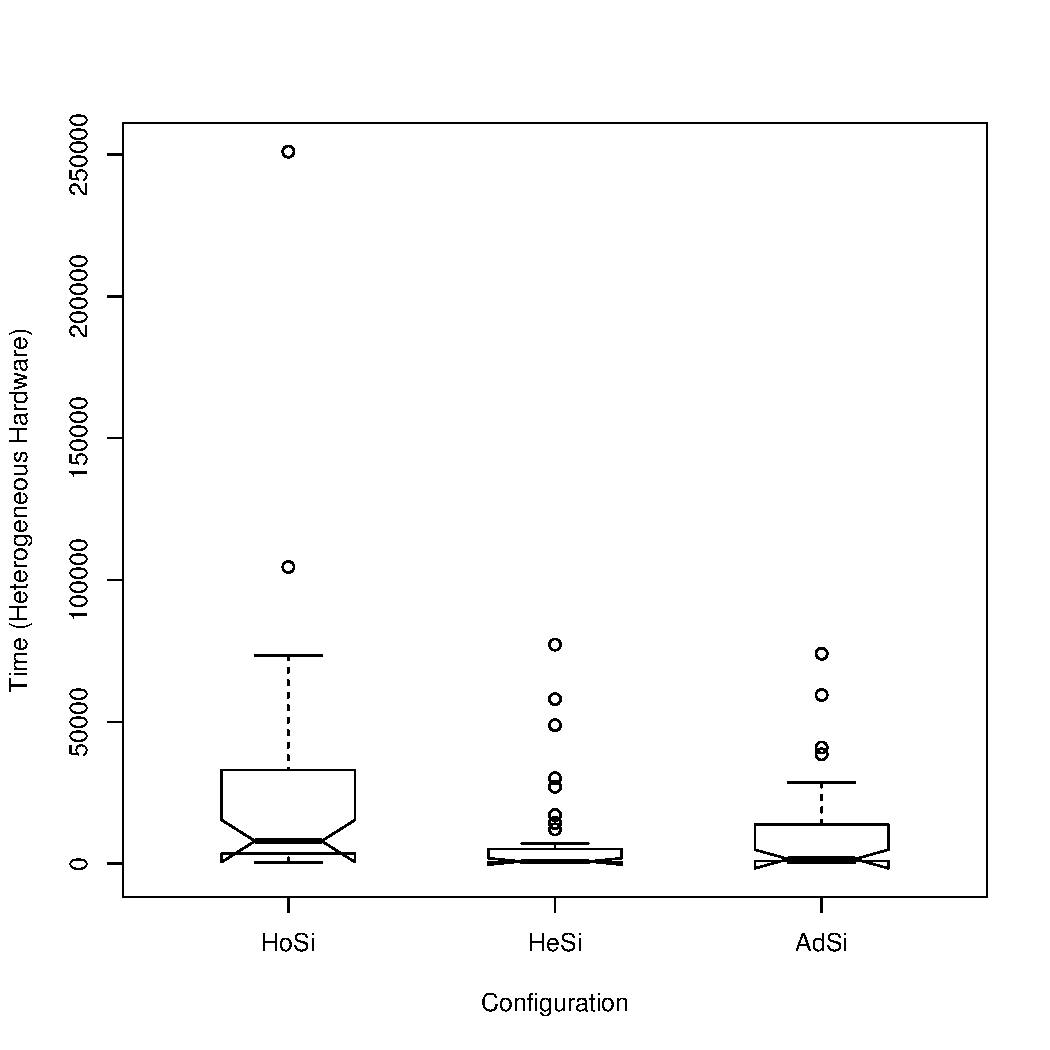
\includegraphics[scale =0.5] {gfx/adaptiveresults/timeMMDPhetero.pdf}
   \label{fig:subfigtimeMMDPhetero}
}
\\
\subfloat[Homogeneous cluster]{
   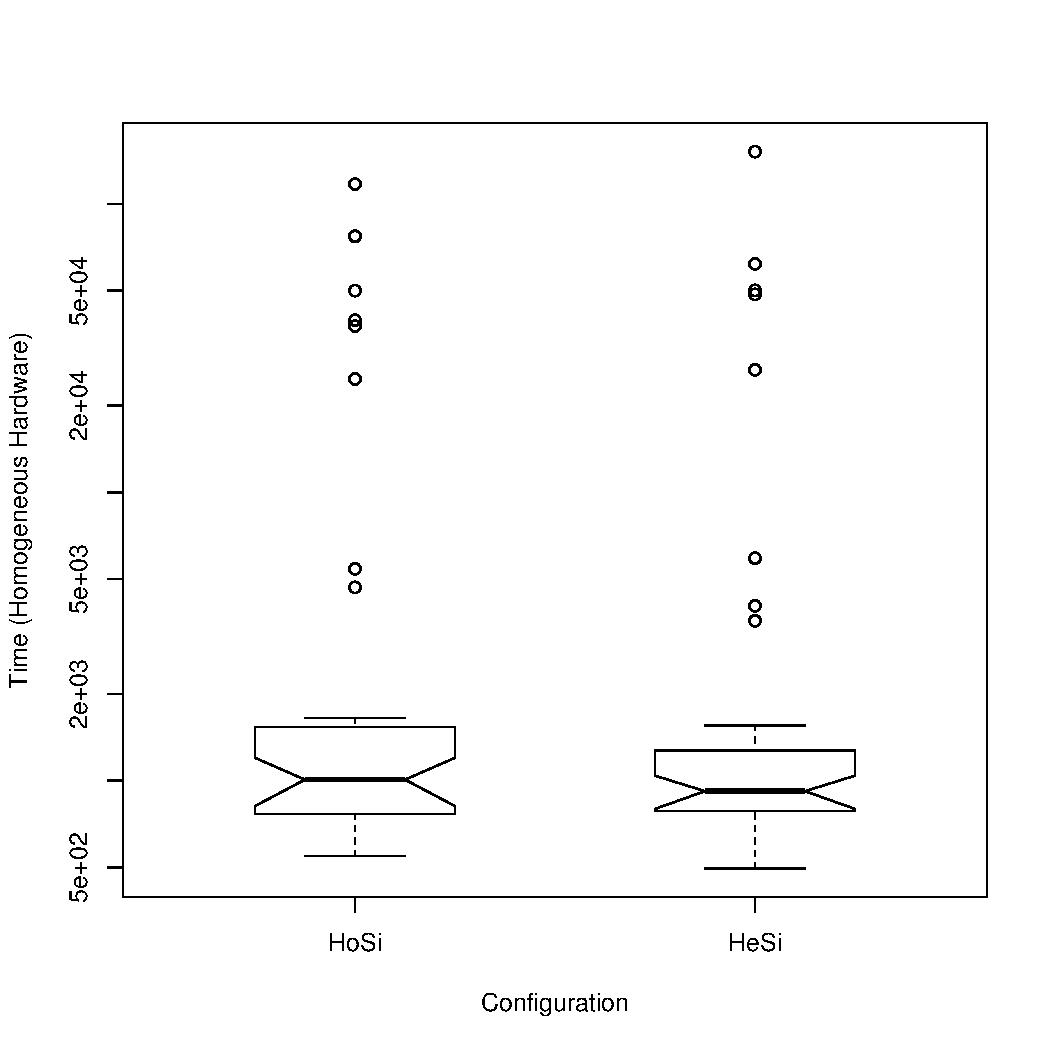
\includegraphics[scale =0.5] {gfx/adaptiveresults/timeMMDPhomo.pdf}
   \label{fig:subfigtimeMMDPhomo}
 }
 \end{tabular}
\caption{Time to obtain the optimum in the MMDP problem
  (milliseconds).}
%En estos gráficos no se ve nada. O cambias la escala para eliminar
%los outliers o los pones logarítmicos - JJ 

\label{fig:timeMMDP}
\end{SCfigure}

\begin{SCfigure}[tb]
\centering
\begin{tabular}{c}
\subfloat[Heterogeneous cluster]{
   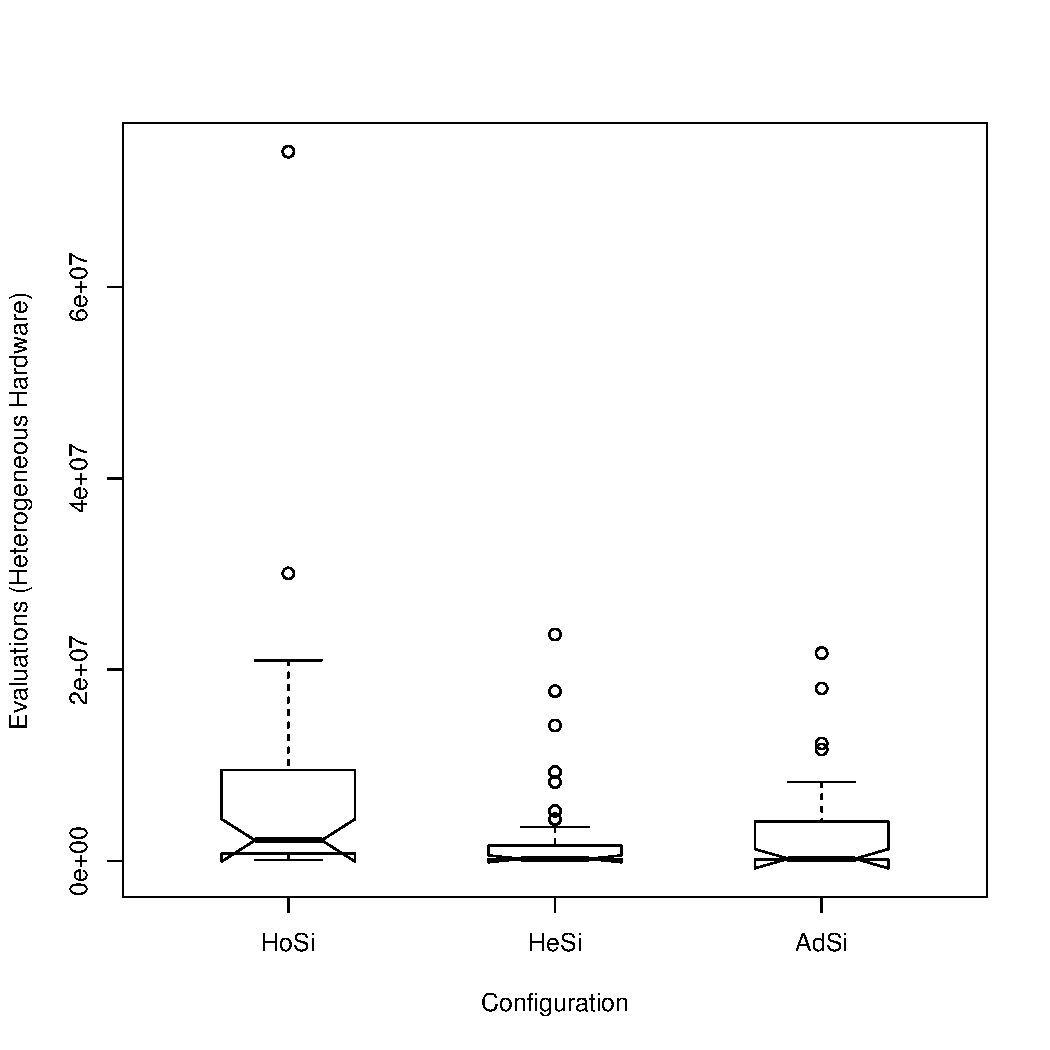
\includegraphics[scale =0.5] {gfx/adaptiveresults/evalsMMDPhetero.pdf}
   \label{fig:evalsMMDPhetero}
 }
 \\
\subfloat[Homogeneous cluster]{
   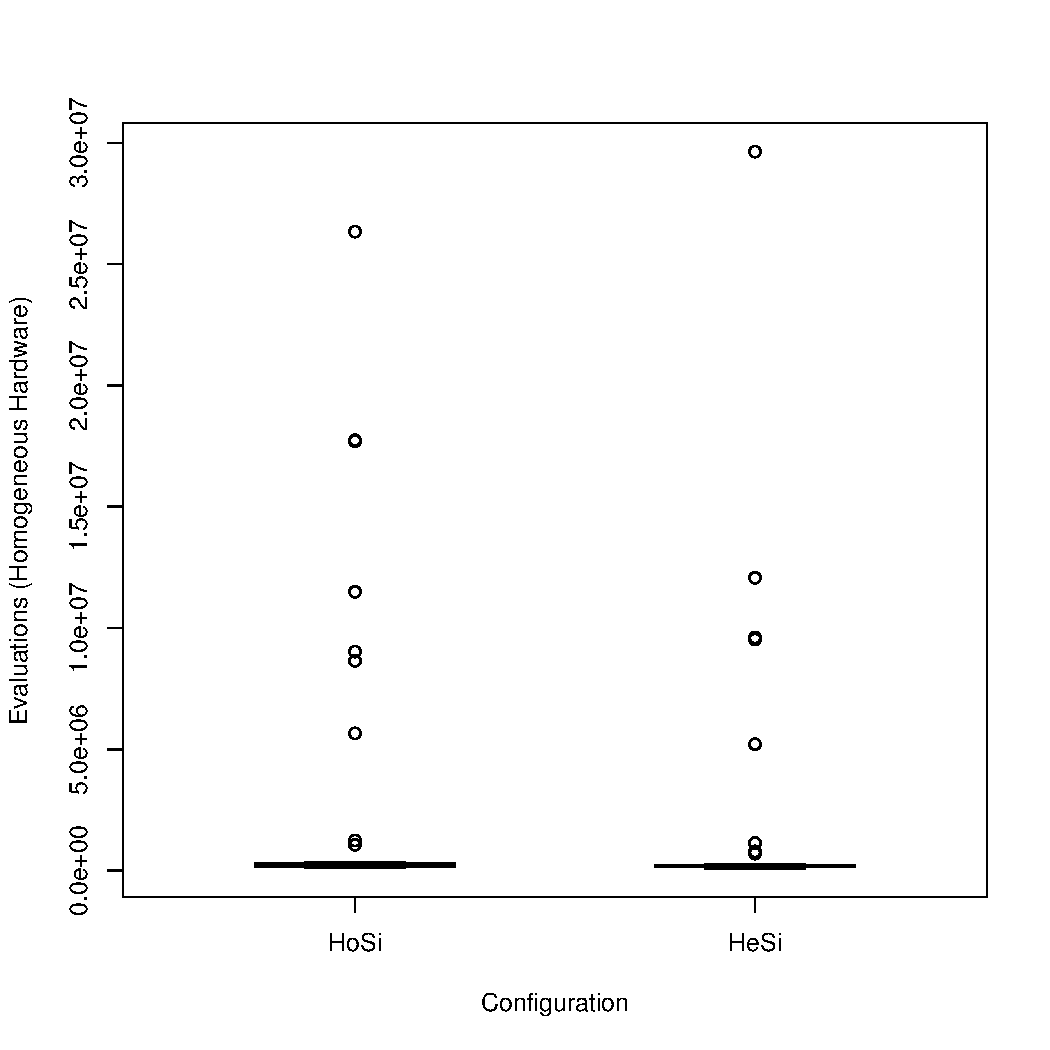
\includegraphics[scale =0.5] {gfx/adaptiveresults/evalsMMDPhomo.pdf}
   \label{fig:evalsMMDPhomo}
 }
 \end{tabular}
\caption{Number of evaluations for MMDP problem.}
\label{fig:evalsMMDP}
\end{SCfigure}



To see the differences on how the evolution is being performed, the
average fitness in each node of HeHa is shown in Figures
\ref{fig:hosiheha} and \ref{fig:hesiheha}. As it can be seen, with the
HeSi (Figure \ref{fig:hesiheha}), the local optima are overtaken in
less time than HoSi (Figure \ref{fig:hosiheha}).  This can be
explained because in HeSi, the migration from HeN4 to HeN1 is
performed faster, adding more heterogeneity to the whole system. Gaps
in the figures correspond to the time spent in the nodes for sending
the migrant individual to other nodes (not while they are receiving
them). %no se entiende - JJ
 In the HoHa configurations, the evolution of sub-population is
 performed at the same time, being the average fitness similar for all
 nodes during all runs.  


\begin{SCfigure}[tb]
\centering
 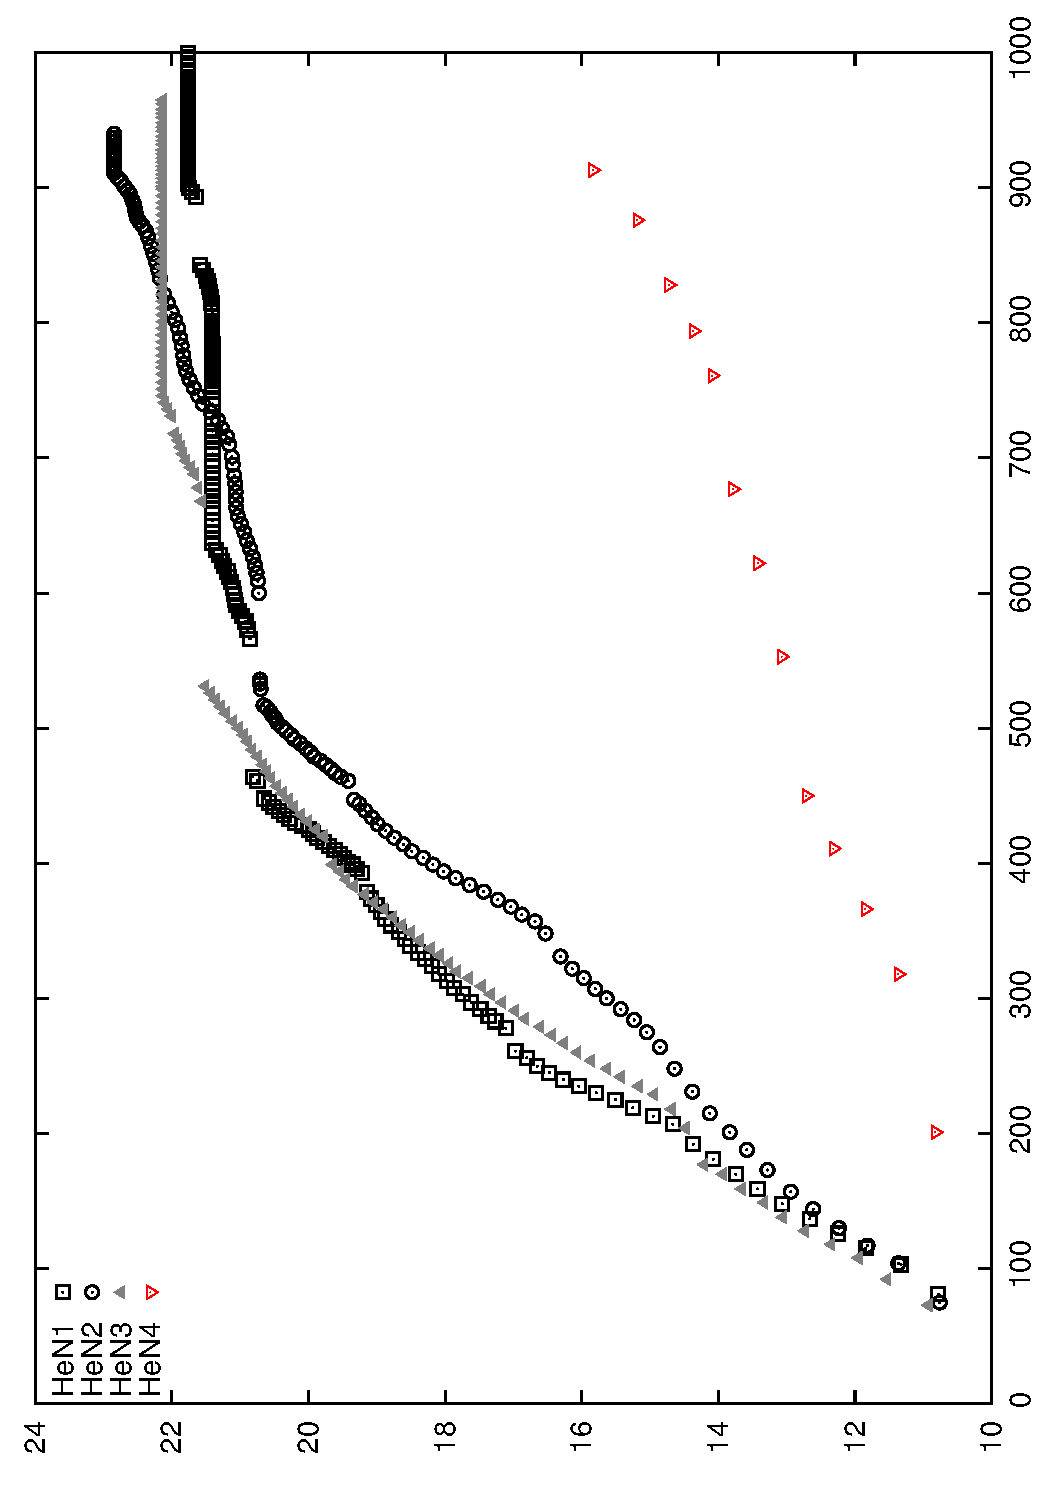
\includegraphics[angle=-90,scale =0.4] {gfx/adaptiveresults/generationsMMDPhomosize.pdf}
\caption{Average fitness in the first 1000 milliseconds of execution of the four nodes of the heterogeneous cluster with the same sub-population sizes (HoSi/HeHa) for the MMDP problem.}
\label{fig:hosiheha}
\end{SCfigure}

\begin{SCfigure}[tb]
\centering
 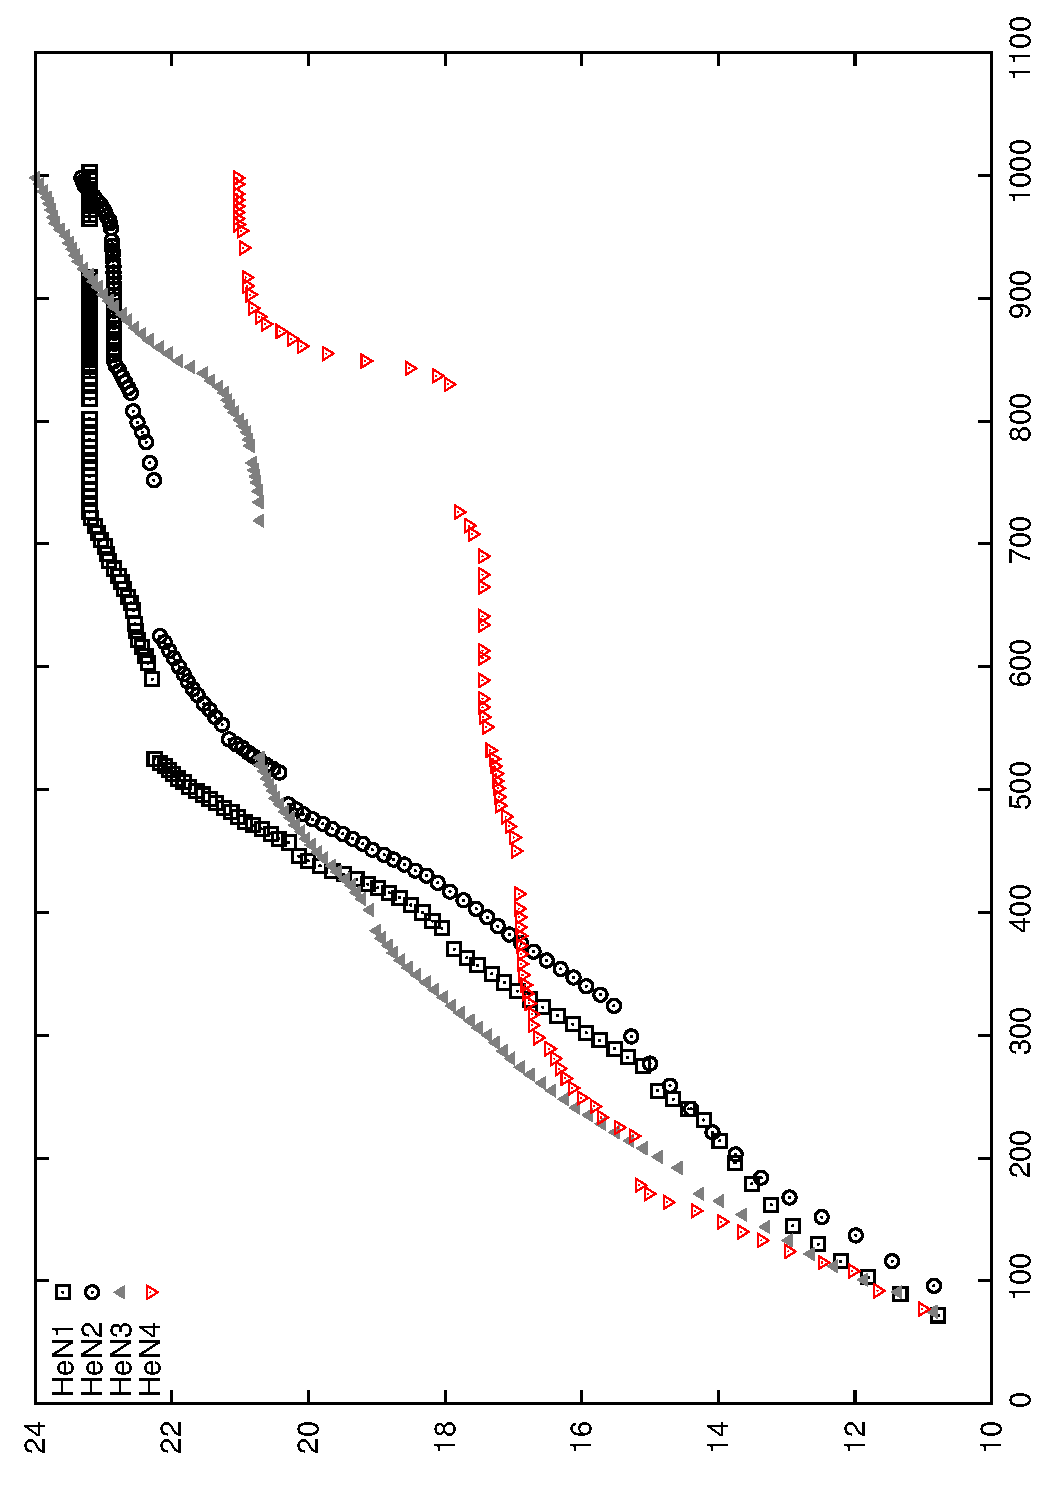
\includegraphics[angle=-90,scale =0.4] {gfx/adaptiveresults/generationsMMDPheterosize.pdf}
\caption{Average fitness in the first 1000 milliseconds of execution
  of the four nodes of the heterogeneous cluster with different
  sub-population sizes (HeSi/HeHa) for the MMDP problem.} % Explica la
                                % leyenda en este pie. ¿Qué diablos es
                                % n1, n2, etc...? - JJ
\label{fig:hesiheha}
\end{SCfigure}

With respect to AdSi/HeHa, %agh, regarding to. ¡Amoragismos no! - JJ
                           %FERGU: a lo mejor lo puso él xD (lo
                           %cambio).
% No es cuestión de cambiarlo, es cuestión de "narrar" lo que quieres
% contar. No se trata de ir contando figura en figura lo que se
% ve. ¿Qué querías probar? ¿En qué contribuye esta gráfica a probarlo?
% ¿Qué tiene que ver todo ello con LA TESIS? - JJ
results are significantly  equal (p-value 0.139) to HeSi/HeHa (and,
therefore, better than HoSi/HeHa), but this time no previous tuning
has been required.  Average sub-population sizes in each node are
shown in Table \ref{table:sizesMMDP}. The proportions of size are
similar to the proportions in Table \ref{table:generations}. Figure
\ref{fig:sizesMMDP} plots all the possible sizes in each node during
all the runs. This figure shows that the variation of the
sub-population sizes lies proportionally to the computational power of
each node. The outliers in boxplots are produced during the size
changing, as it can be seen in Figure \ref{fig:sizesMMDP1ejec}. As N4
is the slower node with difference it keeps its size always close to
the minimum (16 individuals). % ¿Esto es bueno o malo? ¿Qué significa?
                              % ¿Se debe a que es asíncrono? ¿Si no lo
                              % fuera no haría falta que fuera la
                              % población tan pequeña? - JJ 

\begin{SCfigure}[tb]
\centering
 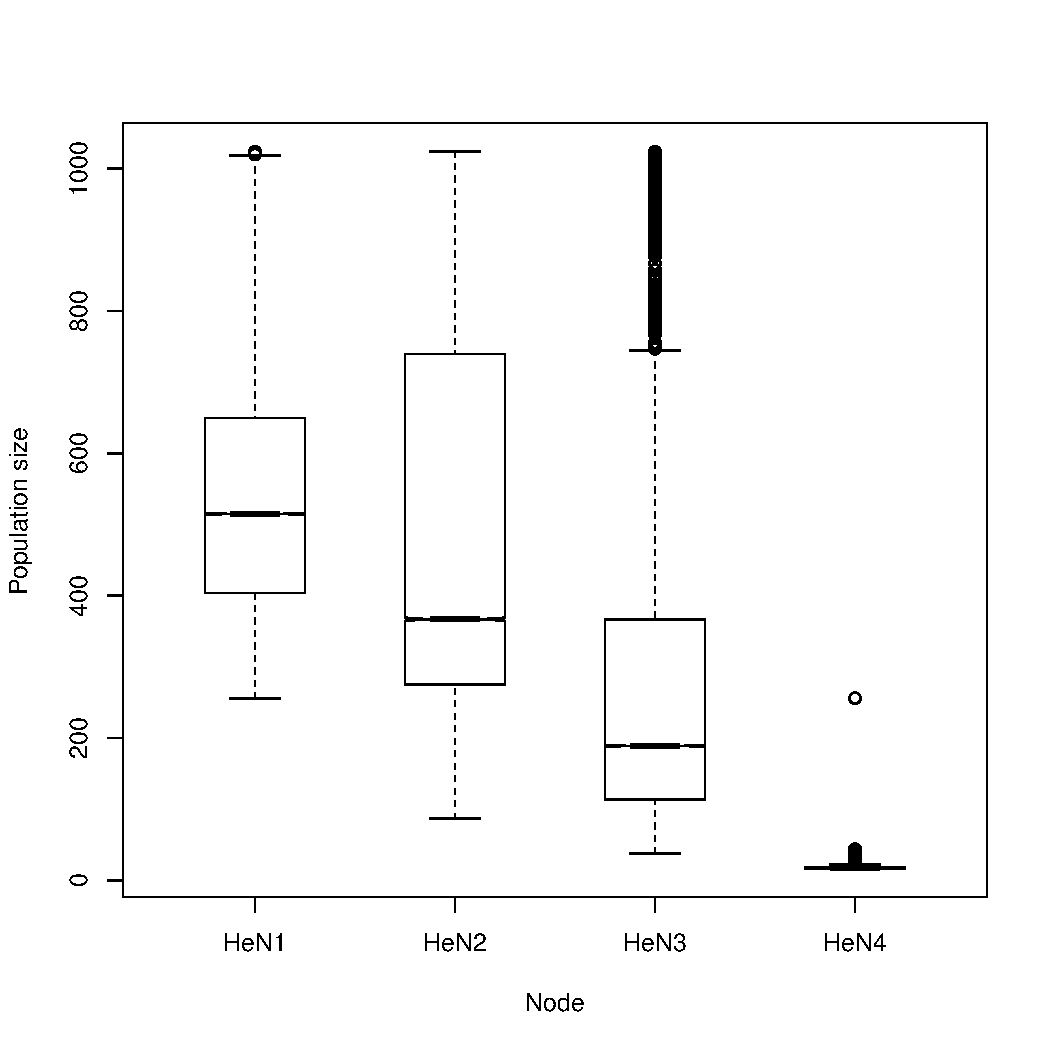
\includegraphics[scale =0.4] {gfx/adaptiveresults/sizesMMDP.pdf}
\caption{Boxplots of the sub-population sizes in each node during all
  the runs for the MMDP problem.} 
%Otra figura, otra terminología, además diferente de la de
%abajo. ¿Esto es population size de qué? ¿Es un resultado? ¿Menor
%poblacióne s mejor? ¿Qué diablos significa el resultado? ¿Final?
%¿Media de cuantas? 
- JJ
\label{fig:sizesMMDP}
\end{SCfigure}

\begin{SCfigure}[tb]
\centering
 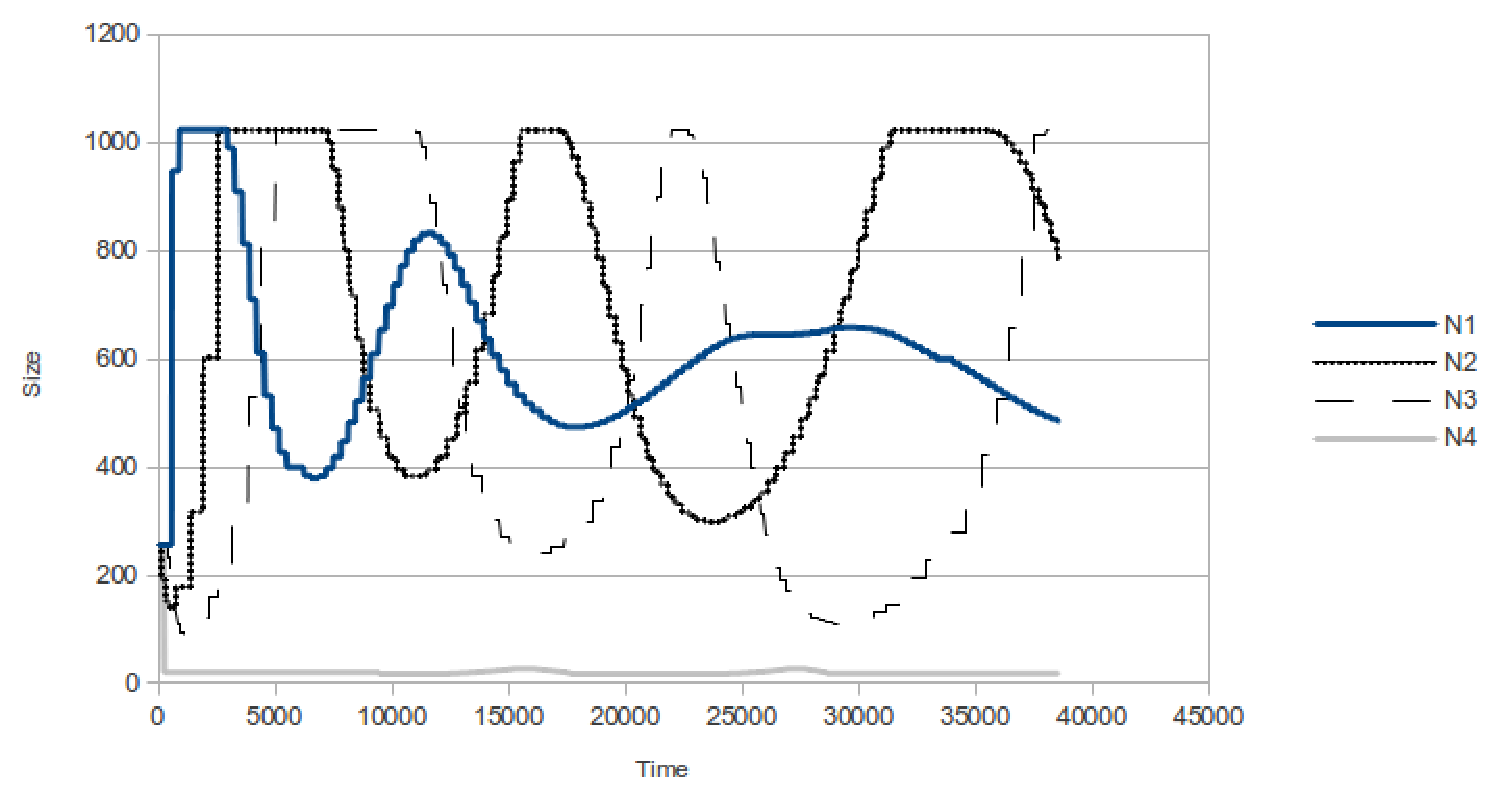
\includegraphics[scale =0.4] {gfx/adaptiveresults/sizesMMDP1ejec.pdf}
\caption{Population size in all nodes during one execution to solve
  the MMDP problem.} % ¿average? ¿Typical? ¿Por qué un nodo se queda
                     % sin nadie? Etiqueta cada nodo con alguna cosa
                     % que signifique algo, como el procesador que
                     % usan o algo - JJ 
\label{fig:sizesMMDP1ejec}
\end{SCfigure}



\begin{SCtable}[][tb]
\resizebox{6cm}{!}{
\begin{tabular}{ccccc}
\hline
\rowcolor{colorCorporativoSuave}Node        & HeN1     & HeN2      & HeN3     & HeN4   \\ \hline \hline
\rowcolor{colorCorporativoMasSuave}Size &  556.31 & 504.30  & 321.15 & 19.81 \\ \hline
\rowcolor{colorCorporativoSuave}Proportion  & 39.69 &  35.98 & 22.91 & 1.41   \\ \hline
\end{tabular}
\caption{Average % over what? -proportion over what? What does it
                 % mean¿ - JJ
sub-population size in each node on the heterogeneous cluster with adaptive size (MMDP).}
\label{table:sizesMMDP}
}
\end{SCtable}



Summarizing, adapting the sub-population sizes to the computational
power of each machine (offline and online) has reduced the time to
obtain the optimum. The same heterogeneous fixed sizes in the
homogeneous cluster does not produce a significant decrease of running
time, so the improvement is produced by the heterogeneity and not due
to the different island sizes. Moreover, the AdSi proposal is not
applicable in HoHa because there are not differences of generations
during runtime. % y esto es interesante porque... - JJ
% y sigues sin decir por qué es interesante y en qué contribuye a
% probar TU TESIS  - JJ 

\subsection{OneMax results}

% REcuerda: ¿qué querías probar? ¿Porqué este problema es importante?
% ¿En qué se diferencia del anterior? 
% ¿PODEMOS DE UNA VEZ SALIR DEL ESQUEMA DE "HE HECHO ESTO Y ME HA
% SALIDO TAL COSA"? - jj
Results  % ¿Qué results?
for this problem are shown in Table \ref{tab:onemaxresults} and Figures  \ref{fig:timeOneMax} and \ref{fig:evalsOneMax}. In this case, adapting offline the sub-population sizes significantly decreases  the running time for solving it in the heterogeneous cluster, but this time, the number of evaluations is increased (see statistical significance in Table \ref{tab:significanceONEMAX}). In the homogeneous system, the effect of changing the sub-population sizes is clearer, and this time the number of evaluations (and therefore, the time) are reduced (both significantly). 

The efficiency to resolve OneMax problem depends mainly on the ability to mix
% ¿onemax es el que es eficiente? ¿resolverlo lo es? - JJ FERGU: arreglado
the building-blocks, and less on the genetic diversity and size of the
population (as with MMDP). No genetic diversity is particularly
required. When properly tuned, a simple Genetic Algorithm is able to
solve OneMax in linear time. Sometimes, problems like OneMax are used
as control functions, in order to check if very efficient algorithms
on hard functions fail on easier ones. As it can be seen in Figure
\ref{fig:gensonemaxhomosize}, the average fitness of all sub-populations
are increasing in linear way in the HoSi/HeHa configuration. However,
the slower node evaluates extremely fewer times.  On the other
side, in Figure \ref{fig:gensonemaxheterosize}, smaller sub-population
sizes make that slower nodes increase the number of evaluations, % make that? increase the? Los nodos lo hacen? ¡Gramática! - JJ
but the average fitness is also maintained in linear way (and in
smaller increase rate) between migrations. Nevertheless, the other
nodes still perform a higher number of evaluations. That is the
reason why the number of evaluations is higher in HeHa, and lower in
HoHa. Computational time is more efficiently spent in faster nodes,
having a higher chance to cross the individuals. %¿so es consecuencia
                                %o causa de lo primero? - JJ
 In addition, due to
the larger size of  individuals in the OneMax problem (5000 bits
vs. 150 of the MMDP), the transmission time is larger, (white gaps in the
figures). % ¿hite gaps qué? - JJ
It also implies that HeN4 sends its best individual to
HeN1 in an extremely large amount of time when using HoSi (every 64
generations). 


\begin{SCtable}[][tb]
\resizebox{11cm}{!}{
\begin{tabular}{ccccc}
\hline
\rowcolor{colorCorporativoSuave}Configuration & Max. generations      & Total generations     &   Total evaluations     & Time (ms) \\ \hline \hline
\rowcolor{colorCorporativoMasSuave}HoSi/HeHa   & 2430.34 $\pm$ 70.16  & 6299.31 $\pm$ 250.87 & 1614673.45  $\pm$  64223.09  &  160713.65 $\pm$   8873.46 \\ \hline
\rowcolor{colorCorporativoSuave}HeSi/HeHa   & 2643.34 $\pm$150.82  & 7969.58 $\pm$214.92 & 1802321.65  $\pm$  30511.96  &  151822.75  $\pm$4764.95 \\ \hline 
\rowcolor{colorCorporativoMasSuave}AdSi/HeHa   & 3698.30 $\pm$ 494.56 & 9465.25 $\pm$ 635.07 & 1149277.43  $\pm$ 58887.13 &  103919.33  $\pm$ 6296.39 \\ \hline \hline
\rowcolor{colorCorporativoSuave}HoSi/HoHa   & 1791.32 $\pm$   31.64& 7111.05 $\pm$125.11 & 1822476.8   $\pm$32029.78  &  141176.1    $\pm$2493.72\\ \hline
\rowcolor{colorCorporativoMasSuave}HeSi/HoHa   & 13698.12 $\pm$ 406.85 & 16012.625 $\pm$  482.61 & 895698.2 $\pm$   29520.99  &  77898.85  $\pm$  2935.57 \\ \hline
\end{tabular}
}
\caption{Results for the OneMax problem.}
\label{tab:onemaxresults}
\end{SCtable}



\begin{SCfigure}[tb]
\centering
\begin{tabular}{c}
\subfloat[Heterogeneous cluster]{
    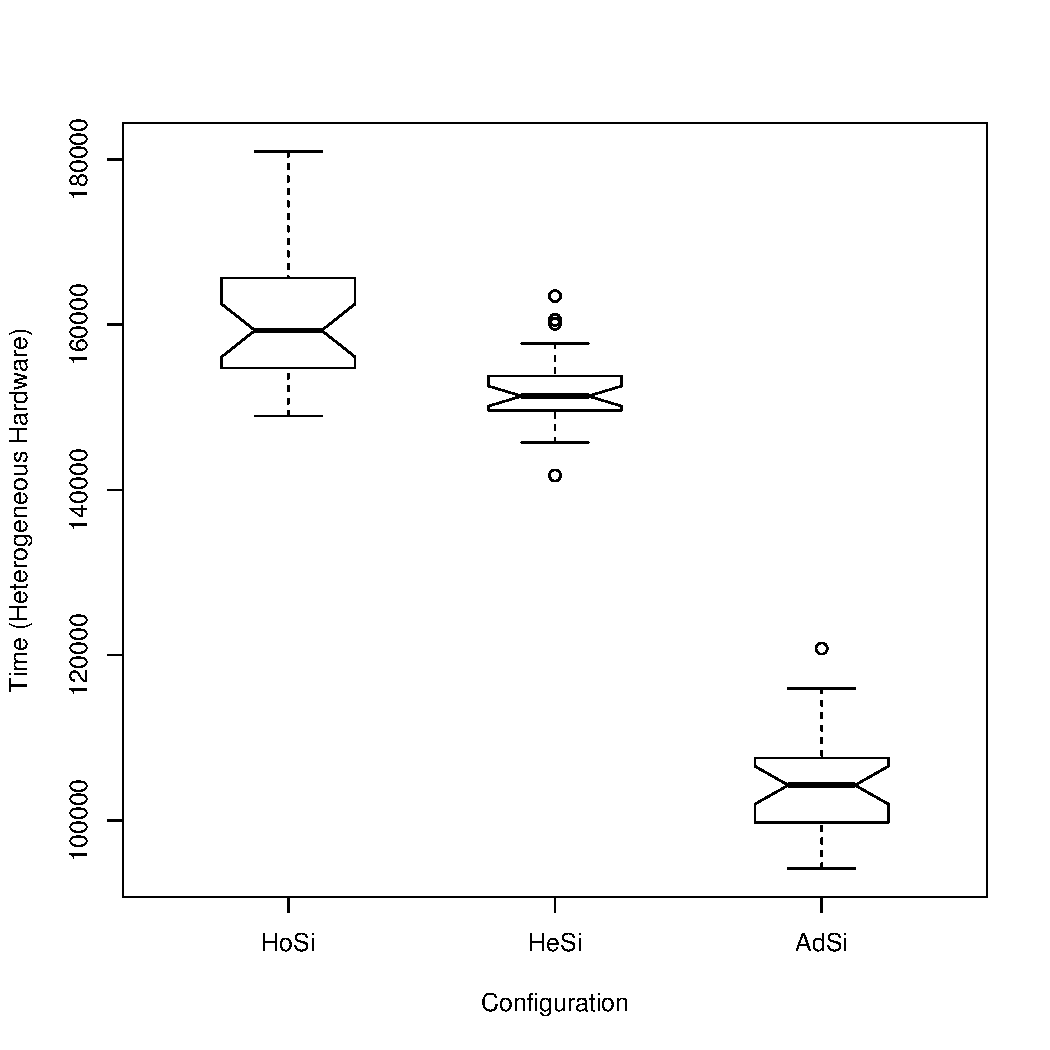
\includegraphics[scale =0.5] {gfx/adaptiveresults/timeONEMAXhetero.pdf}
   \label{fig:timeONEMAXhetero}
 }
 \\
\subfloat[Homogeneous cluster]{
    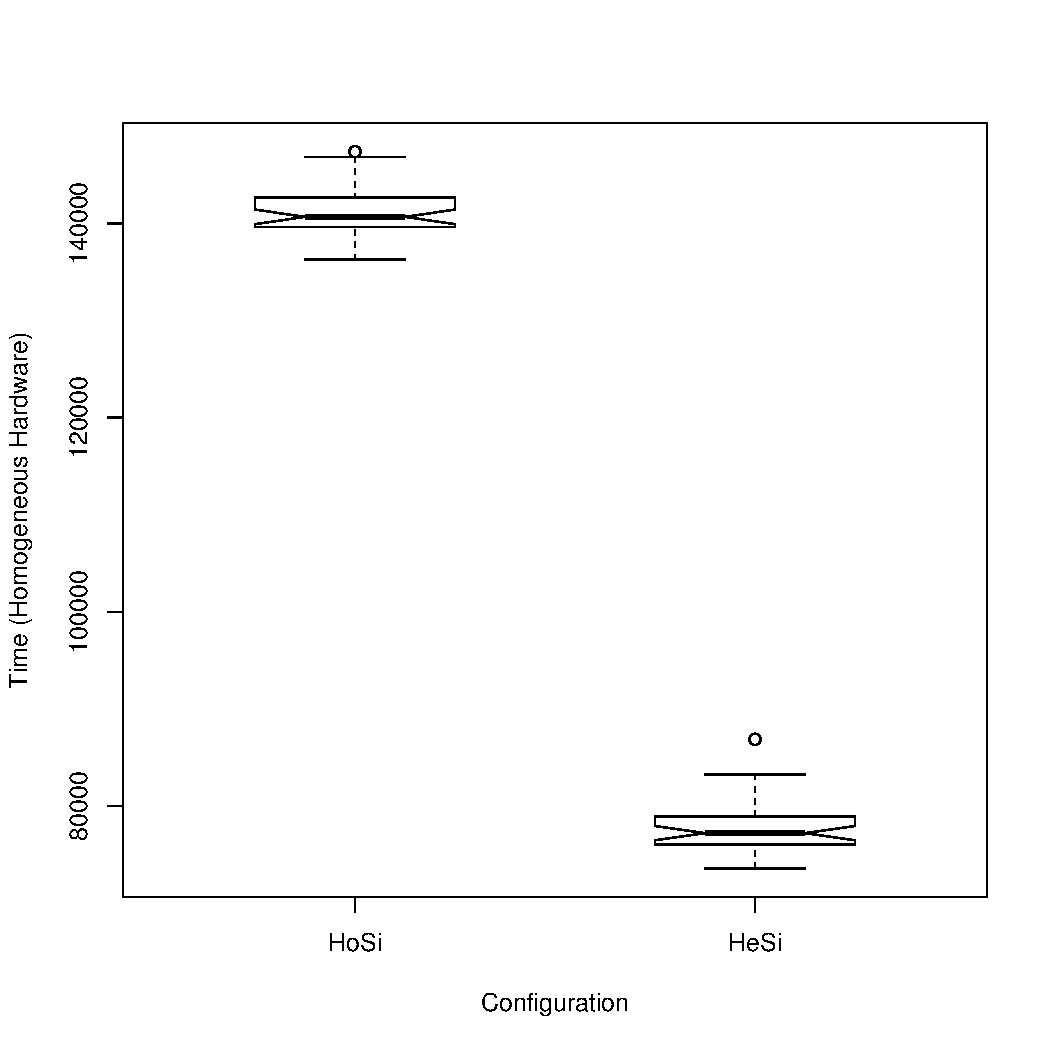
\includegraphics[scale =0.5] {gfx/adaptiveresults/timeONEMAXhomo.pdf}
   \label{fig:timeONEMAXhomo}
 }
 \end{tabular}
\caption{Time to obtain the optimum in the OneMax problem (milliseconds).}
\label{fig:timeOneMax}
\end{SCfigure}

\begin{SCfigure}[tb]
\centering
\begin{tabular}{c}
\subfloat[Heterogeneous cluster]{
   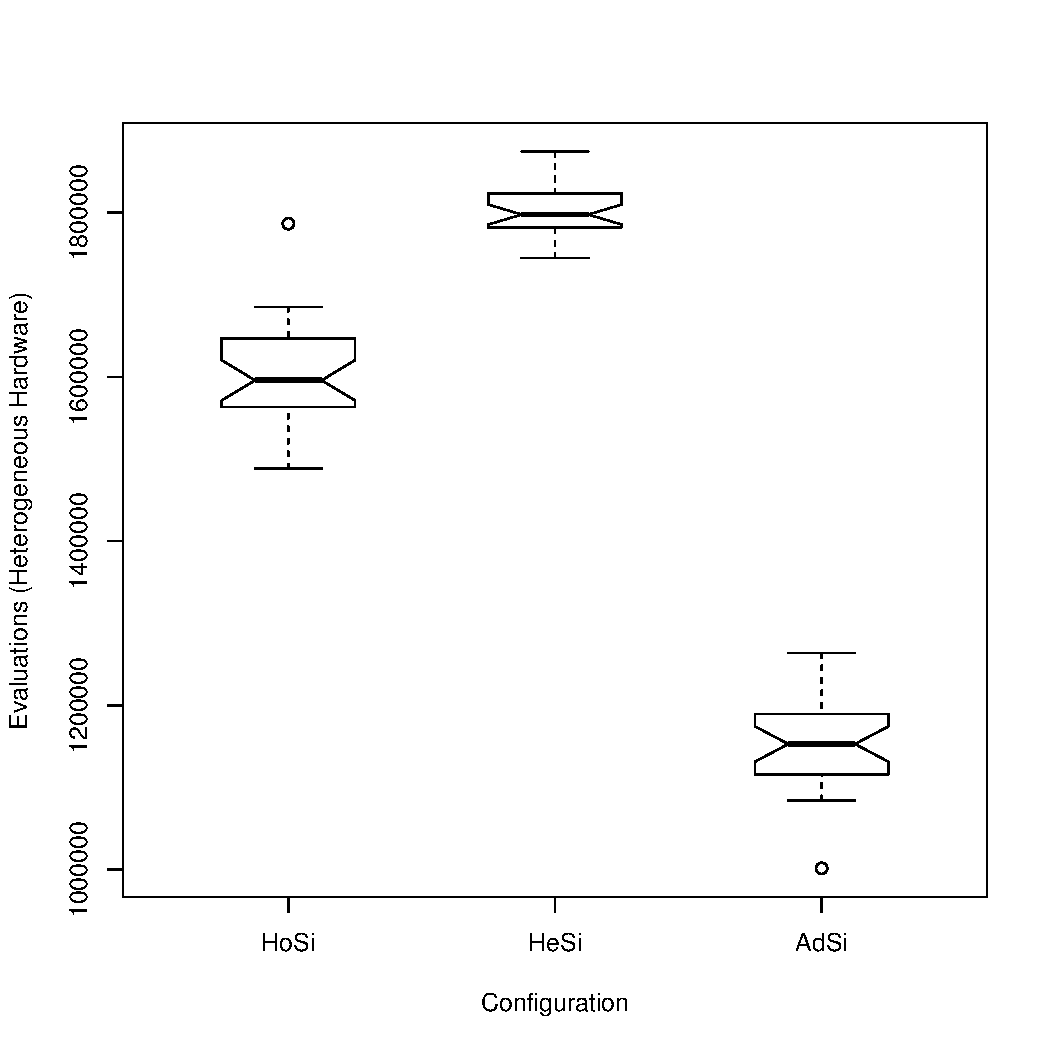
\includegraphics[scale =0.5] {gfx/adaptiveresults/evalsONEMAXhetero.pdf}
   \label{fig:evalsONEMAXhetero}
 }
 \\
\subfloat[Homogeneous cluster]{
   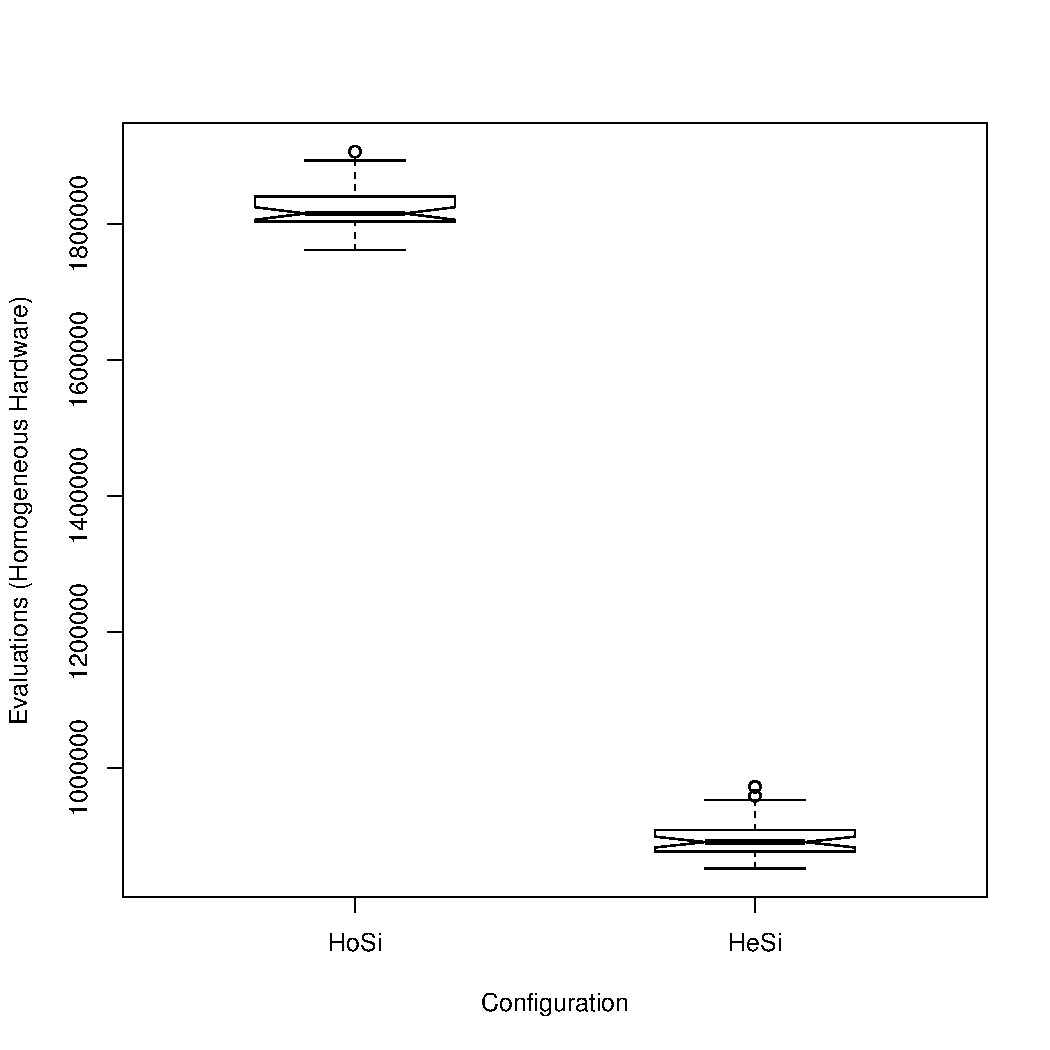
\includegraphics[scale =0.5] {gfx/adaptiveresults/evalsONEMAXhomo.pdf}
   \label{fig:evalsONEMAXhomo}
 }
 \end{tabular}
\caption{Number of evaluations for OneMax problem.}
\label{fig:evalsOneMax}
\end{SCfigure}



\begin{SCfigure}[tb]
\centering 
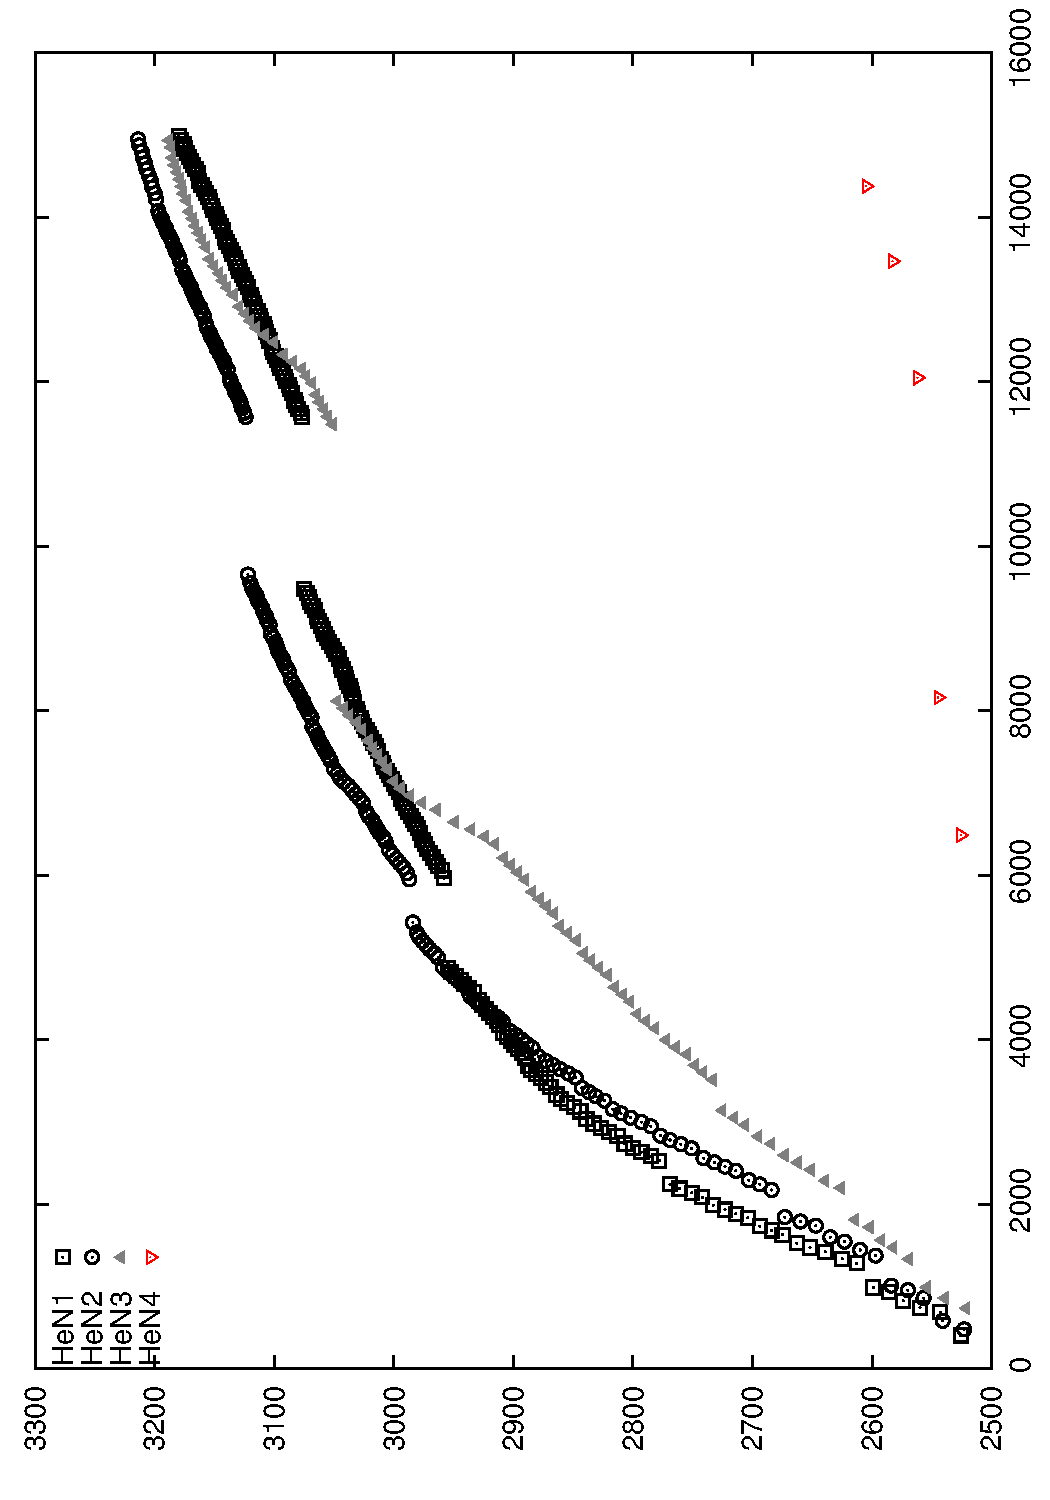
\includegraphics[angle=-90,scale =0.4] {gfx/adaptiveresults/generationsONEMAXhomosize.pdf}
\caption{Average fitness in the first 15000 milliseconds of execution of the four nodes of the heterogeneous cluster with the same sub-population sizes (HoSi/HeHa) for the OneMax problem.}
\label{fig:gensonemaxhomosize}
\end{SCfigure}

\begin{SCfigure}[tb]
\centering
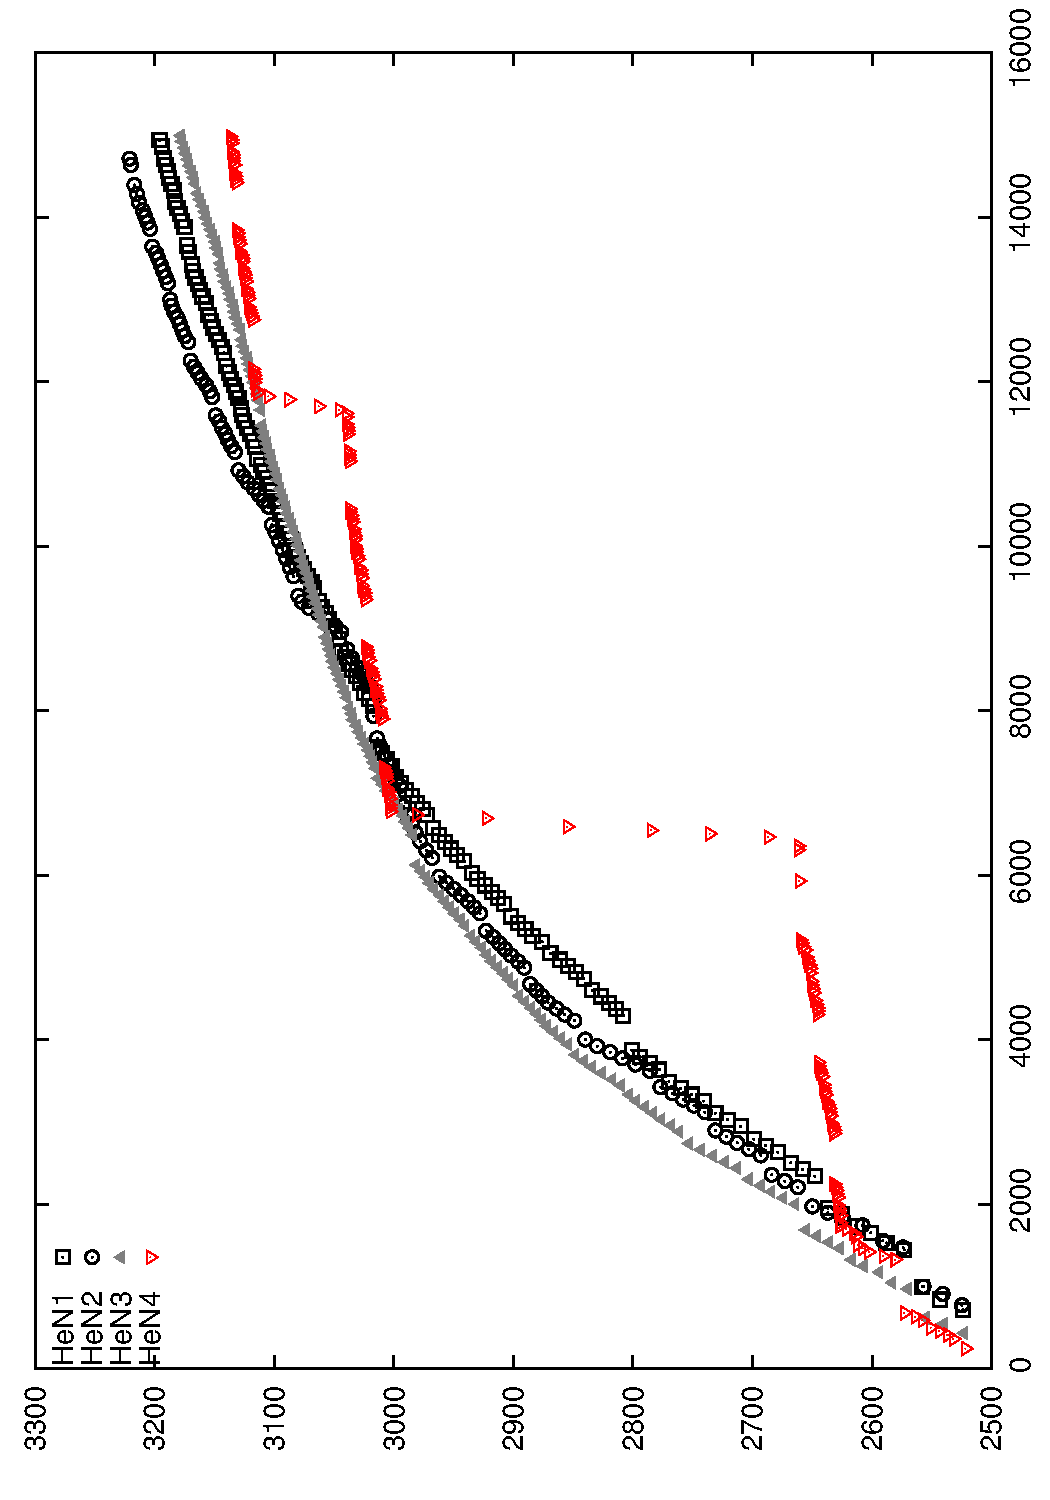
\includegraphics[angle=-90,scale =0.4] {gfx/adaptiveresults/generationsONEMAXheterosize.pdf}
\caption{Average fitness in the first 15000 milliseconds of execution of the four nodes of the heterogeneous cluster with different sub-population sizes (HeSi/HeHa) for the OneMax problem.}
\label{fig:gensonemaxheterosize}
\end{SCfigure}


In the AdSi/HeHa configuration significantly better results in terms of execution time (and number of evaluations) are also attained, and even better than those obtained with HeSi. Average sizes (Table \ref{table:sizesONEMAX}) and boxplots (in Figure \ref{fig:sizesONEMAX}) during all the runs also show proportionality to the computational power of each machine. As in MMDP case, some oscillations (outliers in boxplots) may appear during the execution (as it can be seen in Figure \ref{fig:sizesONEMAX1ejec}).

\begin{SCfigure}[tb]
\centering
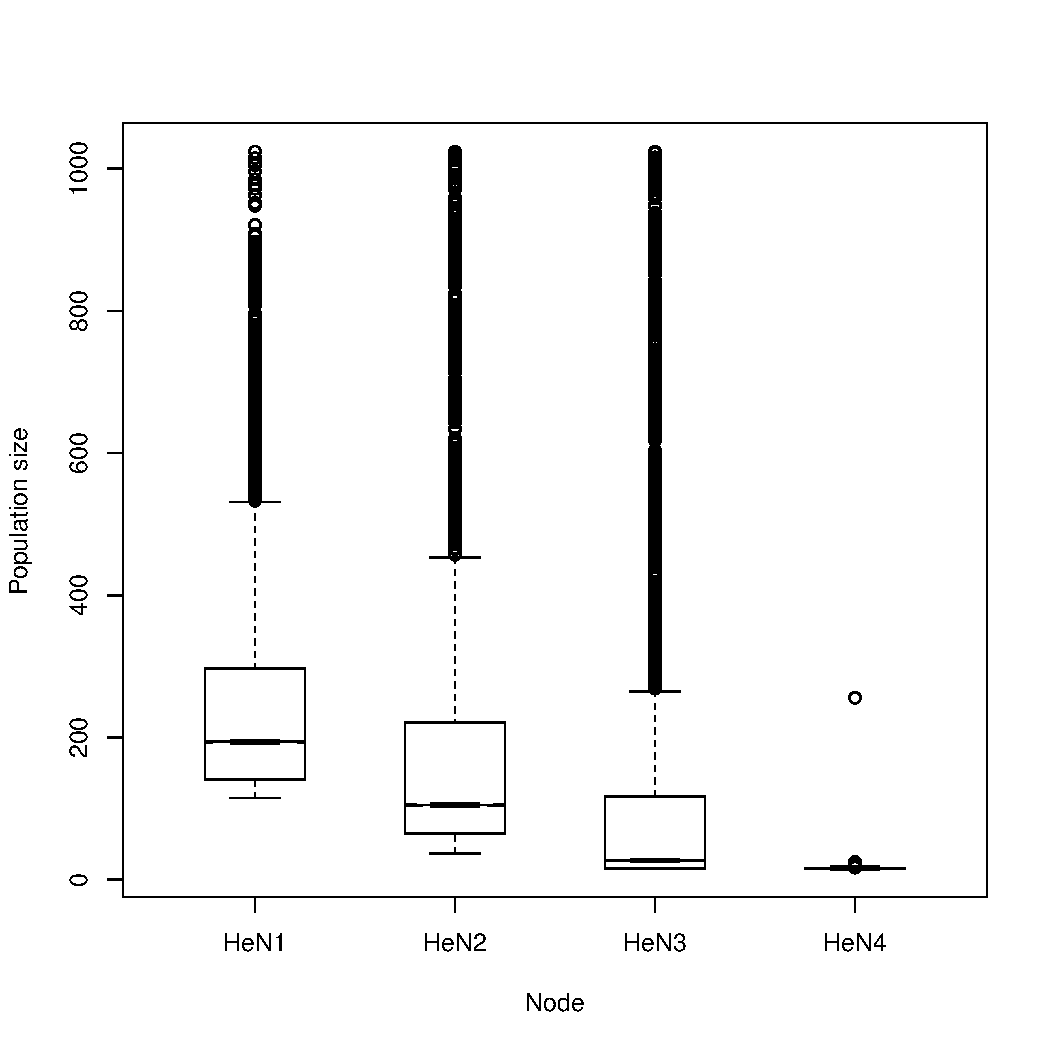
\includegraphics[scale =0.4] {gfx/adaptiveresults/sizesONEMAX.pdf}
\caption{Boxplots of the sub-population sizes in each node during all the runs for the OneMax problem.}
\label{fig:sizesONEMAX}
\end{SCfigure}

\begin{SCfigure}[tb]
\centering
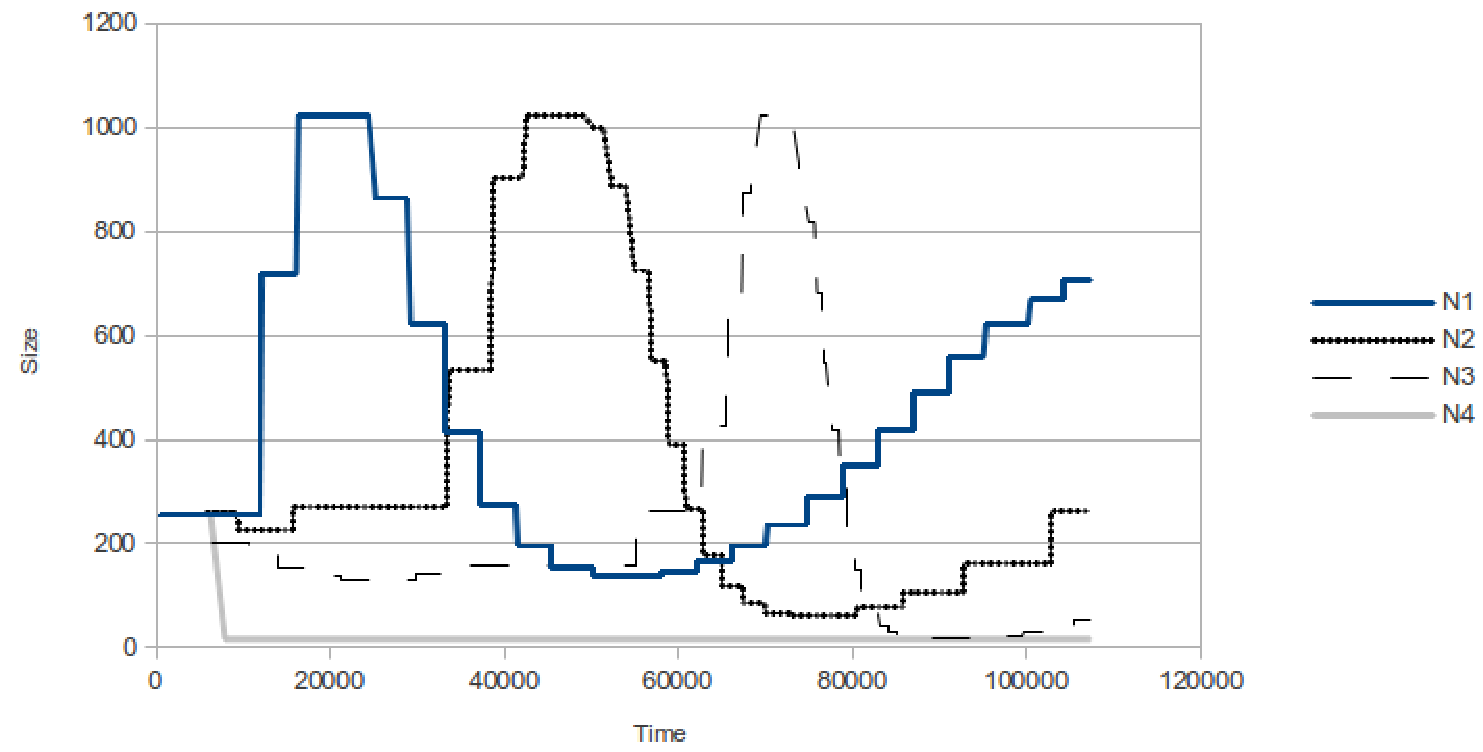
\includegraphics[scale =0.4] {gfx/adaptiveresults/sizesONEMAX1ejec.pdf}
\caption{Sub-population size in each node during one execution to solve the OneMax problem.}
\label{fig:sizesONEMAX1ejec}
\end{SCfigure}


\begin{SCtable}[][tb]
\resizebox{6cm}{!}{
\begin{tabular}{ccccc}
\hline
\rowcolor{colorCorporativoSuave}Node        & HeN1     & HeN2      & HeN3     & HeN4   \\ \hline \hline
\rowcolor{colorCorporativoMasSuave}Size &   267.09 & 158.63 &  74.20  & 16.29 \\ \hline
\rowcolor{colorCorporativoSuave}Proportion  &  51.73 &  30.72 &   14.37 &  3.15  \\ \hline
\end{tabular}
\caption{Average sub-population size in each node on the heterogeneous cluster with adaptive size (OneMax).}
\label{table:sizesONEMAX}
}
\end{SCtable}



\begin{SCtable}[][tb]
\resizebox{11cm}{!}{
\begin{tabular}{cccccc}
\hline

\multicolumn{6}{>{\columncolor{colorCorporativoSuave}}c}{Time} \\ \hline \hline
\multicolumn{6}{>{\columncolor{colorCorporativoMasSuave}}c}{Kruskal-Wallis chi-squared = 20.3042, df = 2, p-value = 3.899e-05} \\ \hline
\rowcolor{colorCorporativoSuave}Configuration       & Test  & obs.dif   & critical.dif  & p-value & difference \\ \hline
\rowcolor{colorCorporativoMasSuave}AdSi/HeHa-HeSi/HeHa      & K-W   & 13.19231  &    18.38851   & 0.1390  &  FALSE \\ \hline
\rowcolor{colorCorporativoSuave}AdSi/HeHa-HoSi/HeHa      & K-W   & 21.11538  &    18.38851   & 0.0067  & TRUE \\ \hline
\rowcolor{colorCorporativoMasSuave}HeSi/HeHa-HoSi/HeHa & K-W   & 34.30769  &    18.38851   & 9\e{-5} & TRUE \\ \hline \hline
\rowcolor{colorCorporativoSuave}HoSi/HoHa-HeSi/HoHa & Wilcoxon & -      & -             & 0.52    & FALSE \\ \hline \hline


\multicolumn{6}{>{\columncolor{colorCorporativoMasSuave}}c}{Evaluations}  \\ \hline \hline
\multicolumn{6}{>{\columncolor{colorCorporativoSuave}}c}{Kruskal-Wallis chi-squared = 11.9676, df = 2, p-value = 0.002519} \\ \hline
\rowcolor{colorCorporativoMasSuave}AdSi/HeHa-HeSi/HeHa      & K-W  & 2.794872   & 18.38851      &  1.0          & FALSE \\ \hline
\rowcolor{colorCorporativoSuave}AdSi/HeHa-HoSi/HeHa      & K-W  & 21.487179  & 18.38851      &  0.0207        & TRUE\\ \hline
\rowcolor{colorCorporativoMasSuave}HeSi/HeHa-HoSi/HeHa & K-W  & 24.282051  & 18.38851      &  0.0028        & TRUE \\ \hline \hline
\rowcolor{colorCorporativoSuave}HoSi/HoHa-HeSi/HoHa &Wilcoxon & -       & -             & 0.08           & FALSE \\ \hline 

\end{tabular}
}
\caption{Statistical significance of the results for MMDP.}
\label{tab:significanceMMDP}
\end{SCtable}


\begin{SCtable}[][tb]
\resizebox{11cm}{!}{
\begin{tabular}{ccccccc}
\hline
\multicolumn{6}{>{\columncolor{colorCorporativoSuave}}c}{Time} \\ \hline \hline
\multicolumn{6}{>{\columncolor{colorCorporativoMasSuave}}c}{Kruskal-Wallis chi-squared = 66.4965, df = 2, p-value = 3.635e-15} \\ \hline
\rowcolor{colorCorporativoSuave}Configuration       & Test  & obs.dif   & critical.dif  & p-value & difference \\ \hline
\rowcolor{colorCorporativoMasSuave}AdSi/HeHa-HeSi/HeHa      & K-W   &  33.27586 &    15.87987   & 2.3\e{-10}  &  TRUE \\ \hline
\rowcolor{colorCorporativoSuave}AdSi/HeHa-HoSi/HeHa      & K-W   &  53.56897 &   15.87987  & $<$2\e{-16}  & TRUE \\ \hline
\rowcolor{colorCorporativoMasSuave}HeSi/HeHa-HoSi/HeHa & K-W   &   20.29310&   15.87987  & 4.2\e{-6}  & TRUE \\ \hline \hline
\rowcolor{colorCorporativoSuave}HoSi/HoHa-HeSi/HoHa & Wilcoxon & -      & -             & 3\e{-8}   & TRUE \\ \hline \hline


\multicolumn{6}{>{\columncolor{colorCorporativoMasSuave}}c}{Evaluations}  \\ \hline \hline
\multicolumn{6}{>{\columncolor{colorCorporativoSuave}}c}{Kruskal-Wallis chi-squared = 75.7342, df = 2, p-value $<$ 2.2e-16} \\ \hline
\rowcolor{colorCorporativoMasSuave}AdSi/HeHa-HeSi/HeHa      & K-W  &  57.72414   &  15.87987     & $<$2\e{-16}          & TRUE \\ \hline
\rowcolor{colorCorporativoSuave}AdSi/HeHa-HoSi/HeHa      & K-W  &  29.27586   &   15.87987    & $<$2\e{-16}         & TRUE\\ \hline
\rowcolor{colorCorporativoMasSuave}HeSi/HeHa-HoSi/HeHa & K-W  &  28.44828   &  15.87987     &  $<$1.3\e{-14}        & TRUE \\ \hline \hline
\rowcolor{colorCorporativoSuave}HoSi/HoHa-HeSi/HoHa &Wilcoxon & -       & -              &  3\e{-8}          & TRUE \\ \hline 

\end{tabular}
}
\caption{Statistical significance of the results for OneMax.}
\label{tab:significanceONEMAX}
\end{SCtable}


% OMG páginas y páginas de tablas y gráficos - JJ

\subsection{Running time analysis}

This sub-section shows the analysis the time spent by each node of the clusters
in every %¿lo haces tú o la subsección? - JJ FERGU: cambiado
 service of the EA for each configuration with fixed sizes (HoSi and HeSi). Tables \ref{tab:mmdptimes} and \ref{tab:onemaxtimes} show the average and standard deviation of the time spent in each stage of the algorithm (He=Heterogeneous cluster, Ho=Homogeneous cluster). Figures \ref{fig:MMDPbars} and \ref{fig:ONEMAXbars} graphically compare these results. As it can be seen, the migration is the most time consuming operation in all configurations, being the migration in HeHa more expensive than in HoHa. This happens because we are using the multi-purpose laboratory network to communicate the nodes, instead of the specific one used in the HoHa system. Note that the standard deviation of the migration is larger in the HeHa cluster because the network is having real conditions of traffic during the experiment. In the MMDP problem (Table \ref{tab:mmdptimes}) changing the sub-po\-pu\-la\-tion size does not affect the migration time, but it affects the rest of the algorithm's stages. However, with larger data communications (individuals of 5000 elements of the OneMax problem), the sub-population size affects the migration time of all nodes. This might be due to the synchronization of migration buffers: if the slowest machine is sending/receiving, bottlenecks can be propagated (as it can be seen in Figure \ref{fig:gensonemaxhomosize}). 

Results also show how the stages of the algorithms depends on the node
of execution. For example, recombination needs more time than mutation
in both problems only in the node HeN4. The reason might be the
creation of new objects (memory allocation), which in Java and in
% en una tesis no se puede decir "might be". Diseñas un experimento
% para probar si esto es cierto o no. Y "diseñas un experimento"
% quiere decir que lo hagas y lo añadas al capítulo - JJ
limited memory (and swapping) requires more time than the iteration of
elements previously created (for example, in the mutation). Adapting
the sub-population size makes the slower node of HeHa behave in similar
way than the other nodes (same time in each stage). Moreover, the size
of the individuals affects to some parts of the EA; for example, in 
OneMax the mutation requires more time than the replacement. However,
it must be taken into account that the duration of each part of the
algorithm is not related to the time to attain the optimum, but rather to
how the diversity and search guidance is maintained in the whole system.  

\begin{SCfigure}[tb]
\centering
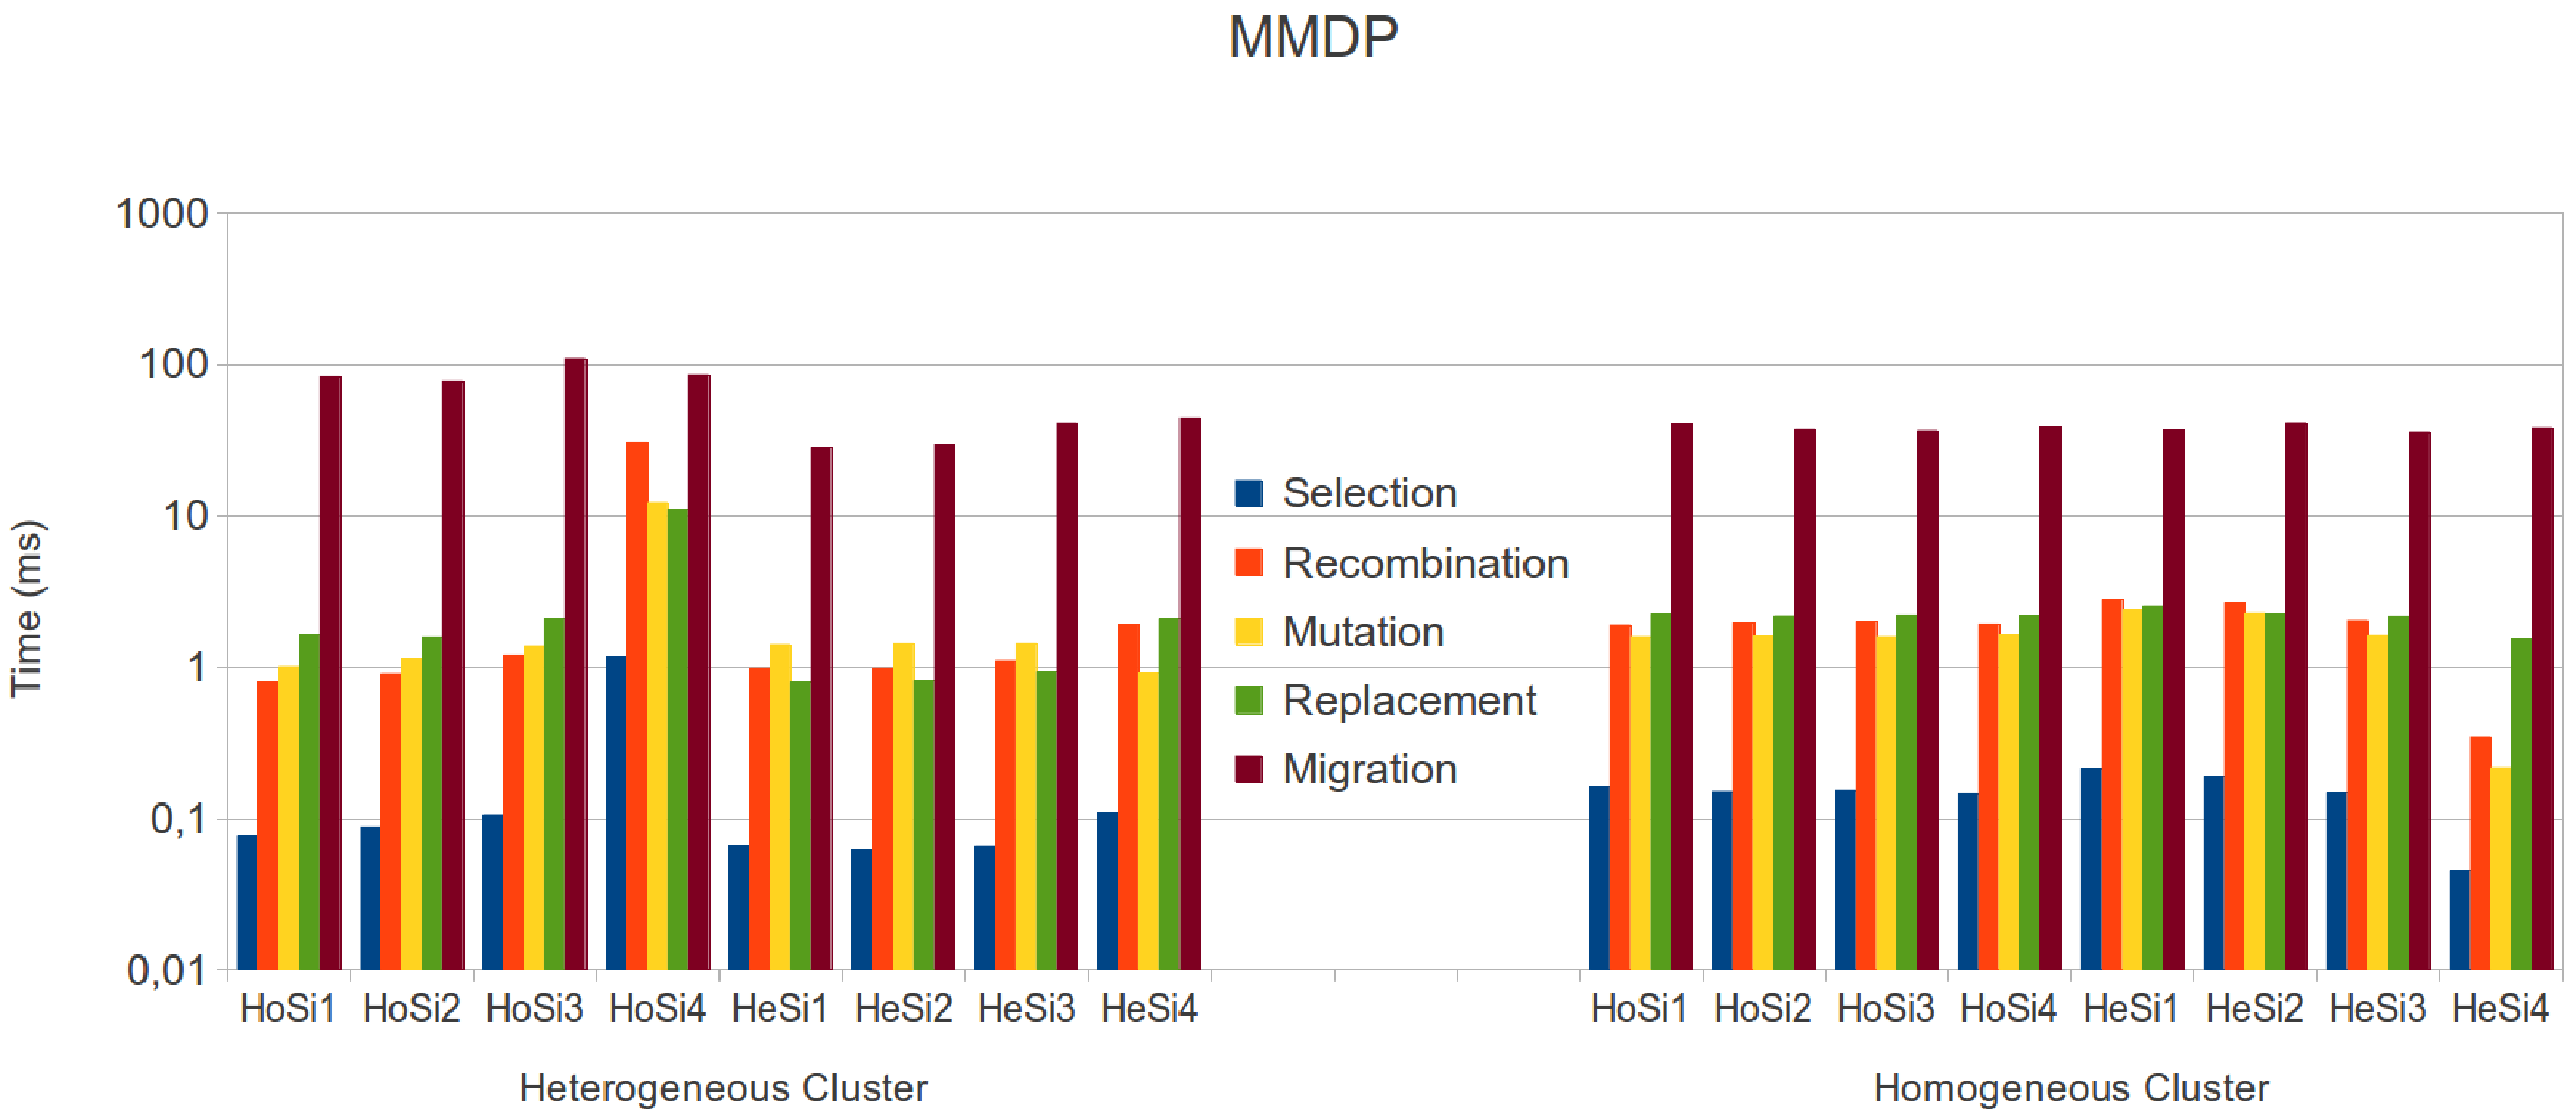
\includegraphics[scale =0.19] {gfx/adaptiveresults/timingMMDP.pdf}
\caption{Average running time in each stage of the algorithm for the MMDP problem.}
\label{fig:MMDPbars}
\end{SCfigure}

\begin{SCfigure}[tb]
\centering
\includegraphics[scale =0.19] {gfx/adaptiveresults/timingONEMAX.pdf}
\caption{Average running time in each stage of the algorithm for the ONEMAX problem.}
\label{fig:ONEMAXbars}
\end{SCfigure}

\begin{SCtable}[][tb]
\resizebox{11cm}{!}{
\begin{tabular}{ccccccc}
\hline
\multicolumn{6}{>{\columncolor{colorCorporativoSuave}}c}{Heterogeneous Cluster} \\ \hline \hline
\rowcolor{colorCorporativoMasSuave}Node    & Selection     & Recombination     & Mutation      & Replacement       & Migration         \\ \hline
\rowcolor{colorCorporativoSuave}HoSi HeN1    & 0.077 $\pm$  0.170 &  0.788  $\pm$ 0.779  & 1.004  $\pm$ 0.187 &  1.648  $\pm$ 20.185 & 82.458  $\pm$ 143.266 \\ \hline
\rowcolor{colorCorporativoMasSuave}HoSi HeN2    & 0.088 $\pm$  0.190 &  0.907 $\pm$  0.932  & 1.145  $\pm$ 0.425 &  1.579  $\pm$ 17.907 & 76.725  $\pm$ 126.360\\ \hline
\rowcolor{colorCorporativoSuave}HoSi HeN3    & 0.105 $\pm$  0.163 &  1.207 $\pm$  0.927  & 1.374  $\pm$ 0.301 &  2.108  $\pm$ 21.848 & 108.605 $\pm$ 142.633\\ \hline
\rowcolor{colorCorporativoMasSuave}HoSi HeN4    & 1.165 $\pm$  1.526 &  30.445$\pm$  59.553 & 12.221 $\pm$ 7.412 &  10.978 $\pm$ 57.135 & 84.936  $\pm$ 0.000\\ \hline \hline
\rowcolor{colorCorporativoSuave}HeSi HeN1    & 0.067 $\pm$  0.065  & 0.973  $\pm$ 0.403 &  1.411 $\pm$  0.166 &  0.790  $\pm$ 6.266 &  28.081 $\pm$ 42.169 \\ \hline
\rowcolor{colorCorporativoMasSuave}HeSi HeN2    & 0.062 $\pm$  0.075  & 0.973  $\pm$ 0.470 &  1.433 $\pm$  0.265 &  0.811  $\pm$ 7.056 &  29.667 $\pm$ 48.702 \\ \hline
\rowcolor{colorCorporativoSuave}HeSi HeN3    & 0.066 $\pm$  0.108  & 1.104  $\pm$ 0.346 &  1.435 $\pm$  0.296 &  0.937  $\pm$ 7.072 &  40.964 $\pm$ 40.027 \\ \hline
\rowcolor{colorCorporativoMasSuave}HeSi HeN4    & 0.109 $\pm$  0.257  & 1.895  $\pm$ 5.611 &  0.913 $\pm$  0.834 &  2.085  $\pm$ 5.626 &  43.880 $\pm$ 7.535 \\ \hline 

\hline \hline
\multicolumn{6}{>{\columncolor{colorCorporativoSuave}}c}{Homogeneous Cluster} \\ \hline  \hline                               
\rowcolor{colorCorporativoMasSuave}Node    & Selection     & Recombination     & Mutation      & Replacement       & Migration \\ \hline
\rowcolor{colorCorporativoSuave}HoSi HoN1    & 0.163 $\pm$  0.223 &  1.884 $\pm$  2.386  & 1.591  $\pm$ 0.479 &  2.254  $\pm$ 5.513  & 40.256  $\pm$ 8.726\\ \hline
\rowcolor{colorCorporativoMasSuave}HoSi HoN2    & 0.151 $\pm$  0.212 &  1.952 $\pm$  2.876  & 1.597  $\pm$ 0.574 &  2.178  $\pm$ 4.922  & 37.110  $\pm$ 6.999\\ \hline
\rowcolor{colorCorporativoSuave}HoSi HoN3    & 0.154 $\pm$  0.206 &  1.990 $\pm$  3.010  & 1.591  $\pm$ 0.577 &  2.215  $\pm$ 4.743  & 36.413  $\pm$ 5.266\\ \hline
\rowcolor{colorCorporativoMasSuave}HoSi HoN4    & 0.146 $\pm$  0.196 &  1.913 $\pm$  2.697  & 1.651  $\pm$ 1.167 &  2.194  $\pm$ 5.124  & 38.429  $\pm$ 6.192\\ \hline \hline
\rowcolor{colorCorporativoSuave}HeSi HoN1    & 0.214 $\pm$  0.288  & 2.800  $\pm$ 3.793 &  2.359 $\pm$  0.691 &  2.516  $\pm$ 4.706 &  36.972 $\pm$ 4.214 \\ \hline
\rowcolor{colorCorporativoMasSuave}HeSi HoN2    & 0.190 $\pm$  0.252  & 2.672  $\pm$ 3.902 &  2.277 $\pm$  0.649 &  2.261  $\pm$ 4.546 &  41.171 $\pm$ 9.672 \\ \hline
\rowcolor{colorCorporativoSuave}HeSi HoN3    & 0.148 $\pm$  0.208  & 2.030  $\pm$ 3.161 &  1.623 $\pm$  0.500 &  2.164  $\pm$ 4.512 &  35.551 $\pm$  6.132 \\ \hline
\rowcolor{colorCorporativoMasSuave}HeSi HoN4    & 0.045 $\pm$  0.052  & 0.345  $\pm$ 1.121 &  0.217 $\pm$  0.142 &  1.531  $\pm$ 4.856 &  38.106 $\pm$ 9.251 \\ \hline
\end{tabular}
}
\caption{Times of the stages of the algorithm for the MMDP problem (in ms).}
\label{tab:mmdptimes}
\end{SCtable}








\begin{SCtable}[][tb]
\resizebox{11cm}{!}{
\begin{tabular}{ccccccc}
\hline
\multicolumn{6}{>{\columncolor{colorCorporativoSuave}}c}{Heterogeneous Cluster} \\ \hline \hline
\rowcolor{colorCorporativoMasSuave}Node    & Selection     & Recombination     & Mutation      & Replacement       & Migration         \\ \hline
\rowcolor{colorCorporativoSuave}HoSi HeN1  &  0.048 $\pm$  0.043  & 18.713 $\pm$ 13.454 & 31.984 $\pm$ 2.104  & 18.375 $\pm$ 197.676 & 1172.986  $\pm$  1108.388 \\ \hline
\rowcolor{colorCorporativoMasSuave}HoSi HeN2  &  0.052 $\pm$  0.051  & 22.266 $\pm$  22.716 & 33.553 $\pm$ 4.931 &  17.176 $\pm$ 180.580 & 1085.508  $\pm$  995.382 \\ \hline
\rowcolor{colorCorporativoSuave}HoSi HeN3  &  0.091 $\pm$  1.005  & 42.634 $\pm$ 21.621  & 47.674 $\pm$ 0.546 &  26.094 $\pm$ 252.667 & 1708.402 $\pm$   1207.925 \\ \hline
\rowcolor{colorCorporativoMasSuave}HoSi HeN4  &  0.851  $\pm$ 0.435  & 1491.568 $\pm$ 1185.723 & 344.872$\pm$ 6.634 &  5.655  $\pm$ 16.175 & 154.019 $\pm$0.000 \\ \hline \hline
\rowcolor{colorCorporativoSuave}HeSi HeN1 &   0.072 $\pm$  0.063 &  32.917 $\pm$ 26.792 & 49.103 $\pm$ 2.655  & 3.023 $\pm$  27.647 & 163.479 $\pm$157.172 \\ \hline
\rowcolor{colorCorporativoMasSuave}HeSi HeN2 &   0.080 $\pm$  0.092 &  43.001 $\pm$ 51.680 & 52.288 $\pm$ 13.210 & 2.527 $\pm$  21.861 & 131.063 $\pm$124.404 \\ \hline
\rowcolor{colorCorporativoSuave}HeSi HeN3 &   0.057 $\pm$  0.052 &  33.951 $\pm$ 15.063 & 41.375 $\pm$ 1.707  & 3.284 $\pm$  30.170 & 186.467 $\pm$163.906 \\ \hline
\rowcolor{colorCorporativoMasSuave}HeSi HeN4 &   0.075 $\pm$  0.107 &  42.443 $\pm$ 88.536 & 16.236 $\pm$ 12.028 & 4.194 $\pm$  33.119 & 131.135 $\pm$144.359 \\ \hline 

\hline \hline
\multicolumn{6}{>{\columncolor{colorCorporativoSuave}}c}{Homogeneous Cluster} \\ \hline  \hline                               
\rowcolor{colorCorporativoMasSuave}Node    & Selection     & Recombination     & Mutation      & Replacement       & Migration \\ \hline
\rowcolor{colorCorporativoSuave}HoSi HoN1  &  0.091 $\pm$  0.078  & 29.969 $\pm$ 21.459 & 47.445 $\pm$ 2.194 &  2.073 $\pm$  6.970 &  38.782 $\pm$ 40.369 \\ \hline
\rowcolor{colorCorporativoMasSuave}HoSi HoN2  &  0.093 $\pm$  0.082  & 30.119 $\pm$ 22.029 & 47.247 $\pm$ 2.146 &  2.108 $\pm$  7.440 &  44.303 $\pm$ 42.759 \\ \hline
\rowcolor{colorCorporativoSuave}HoSi HoN3  &  0.089 $\pm$  0.080  & 30.951 $\pm$ 21.904 & 47.103 $\pm$ 2.031 &  2.138 $\pm$  8.006 &  46.107 $\pm$ 47.351 \\ \hline
\rowcolor{colorCorporativoMasSuave}HoSi HoN4  &  0.098 $\pm$  0.075  & 29.468 $\pm$ 20.876 & 47.086 $\pm$ 1.856 &  2.043 $\pm$  7.491 &  41.458 $\pm$ 44.970 \\ \hline \hline
\rowcolor{colorCorporativoSuave}HeSi HoN1 &   0.144 $\pm$  0.151 &  56.124 $\pm$ 48.229 & 72.811 $\pm$ 5.177  & 2.424 $\pm$  9.056  & 48.165  $\pm$57.798 \\ \hline
\rowcolor{colorCorporativoMasSuave}HeSi HoN2 &   0.141 $\pm$  0.152 &  51.226 $\pm$ 41.016 & 70.047 $\pm$ 4.152  & 2.427 $\pm$  10.890 & 57.152  $\pm$74.177 \\ \hline
\rowcolor{colorCorporativoSuave}HeSi HoN3 &   0.086 $\pm$  0.088 &  26.932 $\pm$ 20.460 & 42.963 $\pm$ 3.935  & 2.239 $\pm$  8.658  & 51.014  $\pm$49.648 \\ \hline
\rowcolor{colorCorporativoMasSuave}HeSi HoN4 &   0.007 $\pm$  0.008 &  1.215  $\pm$ 1.133  & 2.470  $\pm$ 0.098  & 1.553 $\pm$  10.078 & 50.498 $\pm$ 63.983 \\ \hline
\end{tabular}
}
\caption{Times of the stages of the algorithm for the OneMax problem (in ms).}
\label{tab:onemaxtimes}
\end{SCtable}

%AGH! No hay conclusión. ¿Cómo avanza esto la tesis? ¿Qué relación
%tiene con el capítulo siguiente? Todos los capítulos deben tener una
%introducción, una línea argumental y una conclusión - JJ FERGU: es que lo revisaste antes de terminarlo :P (añadidas las conclusiones)

\section{Conclusions}



% No. Tratamos de
                                % probar un objetivo, dilo aquí!!!!!

%Results show that adapting (online or offline) the population size to the computational power of each node in the heterogeneous cluster yields significantly
%better results in time than keeping the same parameter in all
%nodes. This advantage is due to the combination of the heterogeneous
%parameters with the heterogeneity of the machines. % o sea, tener
                                % maquinas heterogéneas y parámetros
                                % heterogéneos es mejor porque usamos
                                % parámetros heterogéneos en máquinas
                                % heterogéneas. Di en qué puede
                                % influir eso en la mejora de los
                                % resultados y discute por qué podría
                                % ser así y propón experimentos para
                                % probar que efectivamente se trata de
                                % eso. - JJ
%On the contrary,
%the same (heterogeneous) parameter setting in all islands of the
%homogeneous cluster could not improve the results than considering the
%same parameter value in all nodes. % ¿Y qué más da?  ¿Por qué es esto
                                % relevante? Di que, por tanto, la
                                % mejora no se debe al cambio de
                                % parámetros sólo, sino a la
                                % combinación entre cambio de
                                % parámetros y adaptación al nodo - JJ 

In this chapter, OSGiLiath has been used to present a study on the adaptation of the sub-population sizes of a distributed EA to the computational power of the different nodes of an heterogeneous cluster.  Different services for migration and algorithm control have been created to be automatically bound. Two adaptation schemes (offline and online) that use information of the computational load of the algorithm have been tested.

Results show that adapting (online or offline) the sub-po\-pu\-la\-tion size to the computational power of each node in the heterogeneous cluster yields significantly
better results in time than keeping the same parameter in all nodes. This advantage is due to the combination of the heterogeneous parameters with the heterogeneity of the machines. On the contrary, the same (heterogeneous) parameter setting in all islands of the homogeneous cluster could not improve the results than considering the same parameter value in all nodes.



Furthermore, changing the sub-population size affects to stages
of the algorithm that are independent of this parameter, such as
the migration. The sub-population size adaptation is also affected by the problem to solve.

In this chapter, as a possible offline parameter setting, we have calculated the computational power of each node proportionally 
to the average number of generations of the homogeneous parameter set. Moreover, a possible way to adapt 
online the sub-population sizes has been performed comparing the current generation with
 the neighbour generation. These results are a promising starting for adapting EAs to the
performance of each execution node with OSGiLiath, using more adequate benchmarks or in a dynamic way. 
% Falta una discusión sobre si las mejoras se deben exclusivamente al
% número de evaluaciones o hay algún otro factor ¿menos overhead?
% ¿nodos más rápidos? - JJ FERGU: no, de hecho el número de evaluaciones no siempre disminuye, lo digo arriba.

%In the future it would be interesting to check the scalability of this approach, using more computational nodes and larger problem instances. In addition, other parameters such as migration rate or crossover probability could be adapted to the execution nodes. Different implementation of these services could be automatically enabled depending of the current state of the EA and the node. Other appropriate benchmark services to analyse the algorithm will be also used to lead to automatic parameter adaptation in runtime (online), with different nodes entering or exiting in the topology, or adapting the parameters to the current load of the system. 

}{\myChapter{Parameter adaptation in heterogeneous machines}\label{chap:adaptive}}
%\ifthenelse{\equal{\value{IncluyeCapitulo}}{2}}{\myChapter{HSV and RGB comparison in Evolutionary Art}\label{chap:art}


\begin{flushright}{\slshape
    I've seen many things, my friend, but you're right:
    \\nothing quite as wonderful as the things you see.} \\ \medskip
    --- {The Doctor. Vincent and the Doctor. Doctor Who.}
\end{flushright}


\minitoc\mtcskip
\vfill




\lettrine{A}{s} part of the \textbf{Objective 4} (\objectiveresearch), in this chapter SOA-EA and OSGiLiath will be used to develop a SOEA. 

The research objective of this application is to study the differences % with respect to what? FERGU: añadido abajo
of using the information of the HSV (Hue, Saturation, Value) and RGB (Red,
Green, Blue) histograms in fitness function during the evolution. Although the two
histograms represent the same information, using HSV (instead as RGB)
as a color model increases the accuracy in image retrieval and
indexing, as explained by \person{Sebe and Lew}
\cite{COLORDIFFERENCES}.






 %A population
%of artistic works (individuals) are evaluated with an aesthetic
%measure to yield a score (fitness). These individuals are combined and
%mutated to generate an offspring with inherited properties of the
%parents, during a certain number of times. % until algo, ¿no? - JJ FERGU: quitado

% Esto es parte de una tesis y como tal tienes que tratarlo. ¿Por qué
% es interesante para la tesis este capítulo? ¿Qué parte de la tesis
% estás probando? - JJ FERGU: añadido



In this chapter, the {\em Processing} \cite{PROCESSING} framework is
integrated inside OSGiLiath % why? En una tesis hay que justificarlo
                            % TODO - JJ FERGU: 
to take advantage of the capabilities offered in image manipulation and analysis. 
{\em Processing} services are then used  to model the
individuals, generate their associate images and extract information
of them (HSV, RGB and Average histograms) to fit with the histograms
of the test images.

% Pero ¿cuál es el objetivo de este trabajo? El objetivo no es evaluar
% arte generativo, porque no se ha aportado nada en ese tema o no está
% claro qué vas a aportar. Es demostrar lo fácil que es adaptar
% Osgiliath a un nuevo problema, midiendo la velocidad de desarrollo y
% ejecución y uso de nuevos entornos como el dichoso processing - JJ FERGU: reescribiendo para que esté relacionado con la tesis


\section{Background}

Evolutionary Art \cite{EART} is a branch of generative art \cite{PHEROGRAPHY}, which is created using a
computer, following the principle of the survival of the fittest, 
using Evolutionary Computation methods.

Metrics such as opinion from humans or image characteristics (for
example, specific combination of colours) can be used to score the
generated images. %We will adopt the latter in this chapter, % why? - JJ
%whose  

%The results of this investigation can help in
%future evolutionary art algorithms, adding the most appropiate color
%model feature with other features available in the literature. For
%example, to be used as one of the features of any kind of
%classifier. % En una tesis el trabajo futuro no viene a cuento. Tienes
            % que evaluar el trabajo de por sí. - JJ FERGU: tienes razón
Computational Aesthetics ``is the research of computational
methods that can make applicable aesthetics decisions in a similar
fashion as humans can'' \cite{COMPAESTH}. In the field of
computational aesthetics, evolutionary systems can play an important
role, by enabling the evolution of aesthetically pleasing or
innovative structures \cite{dipaola2009incorporating}. Evolutionary % y te interesa meterlo como parte de la tesis porque... - JJ
art is characterized by the use of evolutionary principles and natural
selection as a generative process. One of the earliest applications of
evolutionary systems to generate art is the proposal of \person{Sims}
to use an EA to create complex images \cite{sims1991artificial} or
virtual creatures  \cite{sims1994evolving}. In evolutionary art
systems, the evaluation of the aesthetics can be done using human
feedback, with some interactive evaluation of the population, such as
\cite{ashlock2006evolutionary,draves2006electric,moroni2000vox} and
\cite{sims1991artificial}. It also can be achieved by using an
automatic evaluation of fitness, as presented in
\cite{aguilar2008robotic,den2010comparing,dipaola2009incorporating,li2012investigating},
and \cite{sims1994evolving}. % Si lo que quieres hacer es aportar algo
                             % en arte evolutivo, tienes que tomártelo
                             % un poco más en serio, evaluando
                             % artísticamente los resultados,
                             % seleccionando las fotos originales,
                             % buscando arte generativo a base de
                             % bolas similar... No te despistes de tu
                             % objetivo que es el de la tesis - JJ FERGU: tienes razón, esto es qeu lo hicimos entre todos en el hackathon

One of the main challenges in Evolutionary Art is how to measure
aesthetic value of the generated pieces. The source of this difficulty
lies in the inherent complexity, subjectivity and dynamism of
aesthetics. Nevertheless, a wide number of metrics has been
presented. According to \person{Galanter}
\cite{galanter2012computational}, these measures can be classified
into several categories in several pieces of research. The first
category involves the evaluation of the aesthetics of a piece of art
by a formula or principle (e.g., pythagorean proportions). Other
measures apply certain principles of design, such as the rule of
thirds or color theory (e.g., using complimentary colors in Pop Art in
the work of \person{den Heijer and Eiben} \cite{den2012evolving}),
neural networks or complexity measures.   % ¿Cuál vas a usar? No se
                                % trata de hacer "name dropping",
                                % tienes que mencionar lo que sea
                                % interesante o incumba a tu tesis - JJ FERGU: quitadas las morrallas

%This classification also provides a sub-classification for
%evolutionary systems. If aesthetical evaluation is done by human it is
%called {\em interactive} evolutionary systems. Another category is
%performance % utility, más que performance - JJ
% based goals: certain properties of the art piece are evaluated and
% optimized based on performance measures (e.g., usable surface in a
% furniture design generator). Other systems use an exemplar (i.e.,
% real world example) as a way to measure the fitness of the
% individuals. % esto más que arte es diseño, no confundas. Además,
              % ¿cómo se llama esta subclase si la de antes es
              % interactiva? - JJ FERGU: quitando todo
 %Finally, some models use the idea that the complexity is directly
 %related to aesthetics and follow the path firstly stablished in
 %\cite{birkhoff2003aesthetic}.  Given the multidimensional nature of
 %aesthetics judgement, multi-objective EAs are a straightforward
 %option to deal with this multidimensionality. %¿Es lo que vas a usar?
                                %Si no, es que no estás usando lo
                                %"mejor" para tu tesis. - JJ
 %Other extensions to EA, like coevolution or agent swarm behavior, can
 %be used in evolutionary art systems. % ¿Eso es una subclasificación?
                                % ¿Cómo se usan? Una tesis no es un
                                % gran ejercicio de "name dropping",
                                % justifica cosas con enlaces,
                                % intégralas en la narrativa de tu
                                % tesus y sobre todo añade citas. Por
                                % cierto, agent swarm no es una
                                % extensión de EAS- jj FERGU: to fuera

%A brief classification of the aesthetic measures found in the
%evolutionary art systems mentioned in the previous paragraph % NO ESTÁ
                                % EN EL PREVIO, SINO EN EL
                                % ANTERIOR. ¿Por qué no lo pones ahí?
                                % - JJ
% is shown in Table~\ref{table_class}.


%\begin{SCtable}[][t]

%\resizebox{11cm}{!}{
%\begin{tabular}{p{4cm}p{7cm}}
%\hline
%\rowcolor{colorCorporativoSuave}Type & Aesthetic Measure \\ \hline \hline
%\rowcolor{colorCorporativoMasSuave}Formulaic and Geometric Theories & Fractal dimension \cite{den2010comparing}, Image order \cite{li2012investigating}, Benford Law \cite{del2005benford}\\ \hline
%\rowcolor{colorCorporativoSuave}Based on Design Principles &  Color contrast (hue) \cite{den2012evolving},  Color ingredient \cite{li2012investigating}, Composition, tonality and color \cite{dipaola2009incorporating}.\\ \hline
%\rowcolor{colorCorporativoMasSuave}Interactive Evolutionary Computation & The electric sheep project \cite{draves2006electric} \cite{ashlock2006evolutionary,moroni2000vox}\\ \hline
%\rowcolor{colorCorporativoSuave}Error relative to Exemplars &  Resemblance score \cite{dipaola2009incorporating}, pixel comparation \cite{aguilar2008robotic}\\ \hline
%\rowcolor{colorCorporativoMasSuave}Performance based goals & Evolving virtual creatures \cite{sims1994evolving} \\\hline
%\rowcolor{colorCorporativoSuave}Complexity measures & Image complexity \cite{li2012investigating}, Machado and Cardoso aesthetic measure \cite{machado1998computing}\\ \hline
%\end{tabular}
%}
%\caption{Classification of the aesthetic measures used in a brief review of the literature on evolutive art.} 
%\label{table_class} 
%\end{SCtable}

%Several methods for the representation of the art in evolutionary
%art % the _art_ in evolutionary _art_? Seriously? - JJ
% have been proposed. In symbolic expression, the genotype is a tree of
% expressions and the phenotype consists in the image produced  by the
% evaluation of the tree. Shape grammars can also be used as a formal
% description of the image. Previously existing images can be used as a
% basis for the evolution process. Finally, other representations can
% be based on mathematical models, like fractals or cellular
% automata. % Esto ¿a santo de qué? ¿Qué tiene que ver con las
           % clasificaciones? - JJ FERGU: to fuera!


%\rowcolors{2}{gray!25}{white}


% Sin dedicarle una línea a enlazar tu trabajo con el trabajo
% anterior, ni hablar de clasificación, ni de representación, ni de
% por qué avanza el estado del arte ni tu tesis, venga, vamos a hablar
% de processing. Una tesis es una narrativa continua. Aquí el lector
% ya se ha perdido y no entiende a qué viene a cuento toda la parte
% expositiva del capítulo anterior - JJ FERGU: reescribiendo capítulo entero y movido de sitio


%\section{Histograms} % ¿lo ves como antes no hablabas de histogramas? - JJ FERGU: cambiado de sitio

In this chapter.........
The color histograms of 
the images represent the frequency of occurrence of each color
intensities present in the image, by accounting for such sharing
pixels color intensity values. % ¿ein? ¿Google translator? - JJ FERGU: puede ser, porque esto lo escribimos entre varios y a mí no me suena...

The histogram is composed of different ranges or bins that represent a value or set of values of color intensity. % si esto es parte o traslación literal del trabajo, deberías reescribirlo (vas a tener que hacerlo de todas formas para integrarlo con la tesis) - JJ
 The color space is defined as a model representation with respect to color intensity values. Two color models are used in this chapter: RGB (Red, Green, Blue) and HSV (Hue, Saturation and Value). The RGB model is an additive color model in which red, green and blue are added together in different proportions to reproduce a wide range of colors, while the HSV is based on hue or tone, saturation and brightness. While the RGB model is the closest to the way color is processed in some machines, the HSV representation provides a more accurate way to model how humans perceive colors, and also provides more information in image retrieval \cite{COLORDIFFERENCES}.
Figure \ref{fig:histogram} shows the RGB histogram of the image in Figure \ref{fig:flevopark}.

\begin{SCfigure}[20][htb]
\centering
   \includegraphics[scale =0.6] {gfx/art/histogram.png}
\caption{RGB histogram of Figure \ref{fig:flevopark}. }
\label{fig:histogram}
\end{SCfigure}

\begin{SCfigure}[20][htb]
\centering
   \includegraphics[scale =3] {gfx/art/flevopark.jpg}
\caption{Test image to compare with the Fitness functions of our algorithm.}
\label{fig:flevopark}
\end{SCfigure}


\section{Applying SOA-EA}
\label{sec:art:soaea}

\subsection{Identification}

Primitive
ArtisticIndividual
Drawer (individual)
ArtisticInitializer.
ArtisticMutation
ArtisticFitnessCalculator


\subsection{Specification}

The genome of the individual is a list of
primitives. % ¿El genoma es una lista para llevar a cabo los experimentos? ¿En serio? - JJ FERGU: borrado
Each primitive has a position, size and color. This list can
be recombined or mutated (changing the color, position or radium of a
primitive of the list). 


% hala, una subsección con una sola frase. ¿Por qué se
                     % usa esto? ¿Cómo lo enlazas con la literatura?
                     % ¿Fue lo primero que se te ocurrió? ¿Por qué
                     % usas círculos y no cuadrados? ¿O círculos y
                     % cuadrados? ¿O divisiones fractales? ¿O, en
                     % general, cualquier otra cosa? - JJ FERGU: quitada subsección


For this piece of research, we focused on the aesthetics measure of
histogram comparison. The fitness functions are included in the
``Error relative to Exemplars'' category, using \person{Galanter}
\cite{galanter2012computational} classification. The idea is to obtain
an image with the same proportion of tones and colors of a 
existent image. 

% Y eso ¿por qué tendría algo que ver con los valores
                % estéticos de la imagen? Hasta ahora no has
                % justificado que el histograma tenga nada que ver con
                % lo bonita que es - JJ

Three different fitness functions have been implemented:
\begin{itemize}
\item {\em RGB difference}: The difference of the RGB histogram of the individual with the RGB histogram of the test image.
\item {\em HSV difference}: The difference of the HSV histogram of the individual with the HSV histogram of the test image.
\item {\em Average difference}: An average of the two previous differences.
\end{itemize}

RGBFitnes

The range of the these fitness function has been normalized to vary from 0 (totally different histograms) to 1 (the same histogram).

For every color property (i.e., RED, GREEN, BLUE, HUE, SATURATION and VALUE), the histogram is computed using the expression (\ref{eq:histogram}) for each possible value (0-255). Then, again for every property, the difference between the target image and the individual histograms is obtained using (\ref{eq:diff}). Finally, the three fitness are calculated: RGB fitness (\ref{eq:RGB}), HSV fitness (\ref{eq:HSV}) and AVERAGE fitness (\ref{eq:AVERAGE}).

\begin{eqnarray}
  \label{eq:histogram}
  H(c, prop) = \frac{1}{N}\sum_{j=0}^N \left\{\begin{matrix}
1 & prop(j) = c\\ 
0 & otherwise
\end{matrix}\right. \\
\label{eq:diff}
diff(h_1, h_2) = \sum_{j=0}^{255} |h_1(j) - h_2(j)|
\end{eqnarray}
\begin{eqnarray}
  d_R(i) = diff(H(i, RED), H(target, RED))\\
  d_G(i) = diff(H(i, GREEN), H(target, GREEN))\\
  d_B(i) =  diff(H(i, BLUE), H(target, BLUE))\\
  \label{eq:RGB}
  fitness_{RGB}(i) = 1 - 128\frac{d_R(i) + d_G(i) + d_B(i)}{3}
\end{eqnarray}
\begin{eqnarray}
  d_H(i) = diff(H(i, HUE), H(target, HUE))\\
  d_S(i) = diff(H(i, SAT), H(target, SAT))\\
  d_V(i) =  diff(H(i, VAL), H(target, VAL))\\
  \label{eq:HSV}
  fitness_{HSV}(i) = 1 - 128\frac{d_H(i) + d_S(i) + d_V(i)}{3}
\end{eqnarray}
\begin{eqnarray}
  \label{eq:AVERAGE}
  fitness_{AVERAGE}(i) = \frac{fitness_{RGB}+fitness_{HSV}}{2}
\end{eqnarray}




\subsection{Implementation and deployment}



To draw the information contained in the individuals, the {\em Processing} framework has been chosen.
\footnote{\url{http://www.processing.org/}}.  %¿Dónde has justificado el uso de histogramas? Tampoco engañes
      %al lector: Una cosa es Processing y otra los histogramas. Si
      %estamos a processing, estamos a processing - JJ FERGU: reestructurado
 {\em Processing} \cite{PROCESSING} is a framework formed by a simple
 programming language and an integrated development environment (IDE)
 (shown in Figure \ref{fig:ideProc}) primarily created for electronic
 and visual artists such as designers, musicians. This framework has been chosen because it offers
 the following advantages: % No se usa etc en lenguaje formal. Y esto
                           % os lo he dicho en más de mil papers - JJ FERGU: quitados

\begin{itemize}
\item Processing was created for artists, rather than programmers. So, it allows very complex drawings and interactive applications with few lines of code.
\item It is an Open Source software (licensed under the GNU Lesser General Public License), and counts with a large development community.
\item It is based on OpenGL, thus providing 3D acceleration.
\item It also includes more than 100 libraries for video, sound, physics, computer vision and networking.
\item Easy integration with Java, HTML5 and Android.
\end{itemize}

%Lo que estás haciendo es dibujar bolas. las ventajas de processing no
%tienes qu emedirlas de forma absoluta, sino relativa a usar
%simplemente JS con el canvas. En todo caso, siempre se trata de
%ventajas para la tesis. Deja el modo "justificar lo que se me
%ocurrió" y entra en el modo "justificar la tesis" - JJ

\begin{SCfigure}[htb]
\centering

%\subfigure[Processing IDE]{
   \includegraphics[scale =0.55] {gfx/art/Processing.png}
%   \label{fig:subide}
% }
%\subfigure[Runtime of the code.]{
   \includegraphics[scale =0.45] {gfx/art/run.png}
%   \label{fig:subsketch}
% }

\label{fig:ideProc}
\caption{Processing IDE and sketch execution. }
\end{SCfigure}

%However, being a light framework, there exist some disadvantages:
%\begin{itemize}
%\item More complex applications require more programming skills.
%\item The calculations of large computer images are a bit inefficient (although expert programmers can manage OpenGL at low level to fix this).
%\end{itemize} FERGU: esto también lo quito

There exist a lot of interactive artistic projects made with
Processing; examples include art generation, artificial life,
interactive music and other. A good selection can be seen in
\url{http://processing.org/exhibition/}. % Aquí podías citar los
                                % fireworks que hicimos con leonardo
                                % Trujillo - JJ

%Processing is composed by several modules: %En general, cualquier
                                %itemización es mala. Y más cuando,
                                %como esta, suena a copy paste. ¿En
                                %serio que saber que processing tiene
                                %un módulo de tipografía es
                                %interesante para tu tesis? - JJ FERGU: tienes razón, quitado

%\begin{itemize}
%\item Structure: Includes typical programming functions as is the case of return, draw, void, and everything related to the structure of the program.
%\item Environment: Formed by the functions that handle the modeling of the window: cursor, width, height, background, for example.
%\item Data: formed by the data types that make up the different program variables (int, char, float).
%\item Control: Consisting in relations operators.
%\item Shape: it is formed by all functions of the treatment of figures 3D and 2D.
%\item Input: input interactivity features such as functions for the mouse, keyboard or files.
%\item Output: output interactivity features such as write on the screen, save the image or serial control.
%\item Transform: transformations such as rotations or translations.
%\item Lights and Cameras: Functions for the treatment of the lights and cameras.
%\item Color: Functions to handle color of the figures.
%\item Image: Functions for loading images or textures.
%\item Rendering: Functions for rendering images.
%\item Typography: Functions for dealing with text.
%\item Math: Functions for dealing with all mathematical functionality.
%\end{itemize}

{\em Processing} % usa alguna tipografía para diferenciar processing la librería de processing el verbo - JJ FERGU:
can be integrated with Java just by adding a {\em jar} (a
Java library) to existing software.

A new {\em bundle} called OSGiLiART has been
added to the publicly-available source code of OSGiLiath \footnote{\url{https://github.com/fergunet/osgiliath/tree/master/OSGiLiART}}.  % URL - JJ FERGU: Done
Then, using the packages available in the {\em Processing} library an algorithm can generate individuals, manipulate images or extract information. The service {\em Drawer} has been implemented with  {\em ProcessingDrawer}). To create random individuals we have implemented the {\em ArtisticInitializer} to generate individuals composed by the primitives in {\em Processing}. The implementation {\em ArtisticMutator} modifies randomly one of the elements of the individual. Finally, several {\em FitnessCalculator} implementations have been added: {\em HSVFitnessCalculator}, {\em RGBFitnessCalculator} and {\em AverageHistogramFitnessCalculator}. These fitness are explained in next section. There is not necessary to modify other existent service implementations (such as existent Recombinators or Replacers explained in previous chapters), because the abstract design of OSGiLiath.





%\noindent This section shows how Processing has been used in the EA,
%the individual representation, the fitness functions, and the
%parameters of the experiments. % Una tesis debe ser también una metodología. ¿Esta metodología coincide con la del resto de los capítulos? - JJ FERGU: quitado










\section{Experimental Results}
\label{sec:results}

A steady-state evolutionary algorithm has been used. % ¿Por qué? ¿No
                                % es Osgiliath tan flexible? ¿Por qué
                                % no pruebas 7 tipos diferentes?
                                % Tienes que demostrar que conoces los
                                % algoritmos subyacentes.
% A partir de aquí paso de decirte que justifiques cada decisión
% individual. UNA TESIS ES UNA TESIS. Tienes que justificar todo, y
% quiero decir todo (estoy viendo desde aquí la tasa de crossover, por
% ejemplo) en función de tu conocimiento del estado del arte y la
% metodología que estés proponiendo en la tesis.
Each individual is randomly generated at the initialization of the EA. The genome size is 50 elements (circles of maximum radium of 128 pixels). Population size has been set to 32 individuals. Uniform crossover rate is 0.5, and a binary tournament has been chosen for selection (that is, a pool of 16 parents is selected and crossed). Mutation probability is 0.04 (the usual value of {\em 1/genomesize}). Finally, the image size for each individual is 256x256 pixels. The individuals have been compared with the histograms obtained from the image of Figure \ref{fig:flevopark} to guide the evolution. 

 Because of the stochastic nature of the EAs, each algorithm
has been executed 30 times for each different fitness formula. Table
\ref{tab:results} shows the average differences (and standard
deviation) attained with each fitness used. As can be seen, using the
HSV histogram differences as fitness produces a higher RGB similarity
(and therefore, average) than using the RGB or Average
fitness. However, using the average between the two histogram
differences produces higher similarity in HSV (0.294) than only taking
into account the HSV. The maximum fitness is around 25\% of similarity
with the original image since the individual is a list of 50 circles,
and therefore, only a maximum of 50 different colors are used (while
in the original jpg image can be more than millions). See the
histogram of a generated best individual by the algorithm in Figure
\ref{fig:histoind}. An example of evolution for each fitness can be
seen in Figure \ref{fig:rgbgens}, \ref{fig:hsvgens} and
\ref{fig:averagegens}. Comparing with the RGB histogram as fitness, a
bigger fluctuation in the HSV is produced (Figure
\ref{fig:rgbgens}). This can be explained because the RGB information
tends to be more noisy than HSV information: in fact, in
\cite{COLORDIFFERENCES} authors explain the problems this histogram
offers with respect to HSV in image retrieval. Although there is the
same information modeled in both histograms, the transformation from
one to another is not linear, so there is no relation with the
histograms of individuals generated during the evolution. 

\begin{SCtable}[][t]
\resizebox{11cm}{!}{
\begin{tabular}{ccccc}
\hline
\rowcolor{colorCorporativoSuave}Differences used  in Fitness & Obtained RGB      & Obtained HSV  & Obtained Average \\ \hline \hline
\rowcolor{colorCorporativoMasSuave}RGB Histogram    & 0.267 $\pm$ 0.012	& 0.170 $\pm$ 0.010 	& 0.218 $\pm$ 0.009	\\ \hline
\rowcolor{colorCorporativoSuave}HSV Histogram    & 0.227 $\pm$ 0.017	& 0.265 $\pm$ 0.021	& 0.246 $\pm$ 0.010 \\ \hline
\rowcolor{colorCorporativoMasSuave}Average Histogram& 0.173 $\pm$ 0.012	& 0.294 $\pm$ 0.013	& 0.234 $\pm$ 0.010 \\ \hline
\end{tabular}
}
\caption{Results for the different fitness (average of the 30 executions and standard deviation). Only one histogram type is used for fitness calculation, but the other values obtained are also added.}
\label{tab:results}
\end{SCtable}

\begin{SCfigure}[20][htb]
\centering
   \includegraphics[scale =0.6] {gfx/art/individuohist.png}
\caption{RGB histogram of a solution generated by the algorithm.}
\label{fig:histoind}
\end{SCfigure}

\begin{SCfigure}[20][htb]
   \includegraphics[angle=-90,scale =0.40] {gfx/art/rgbgens.png}
\caption{Evolution of the difference in RGB histogram of the best individual compared with the test image. }
\label{fig:rgbgens}
\end{SCfigure}

\begin{SCfigure}[20][htb]
   \includegraphics[angle=-90,scale =0.40] {gfx/art/hsvgens.png}
\caption{Evolution of the difference in HSV histogram of the best individual compared with the test image. }
\label{fig:hsvgens}
\end{SCfigure}

\begin{SCfigure}[20][htb]
   \includegraphics[angle=-90,scale =0.40] {gfx/art/averagegens.png}
\caption{Evolution of the difference of average of RGB and HSV histogram of the best individual compared with the test image. }
\label{fig:averagegens}
\end{SCfigure}

The best individuals obtained are shown in Figure
\ref{fig:bestinds}. Note that, although the numeric fitness is
similar, they produce different color tones. This can be explained for
the limitation of colors used in the individual representation, as
previously said, or the noisy characteristic of the RGB
histogram. Figure \ref{fig:collage} shows one evolution of the best
individual using the HSV fitness in the first 64 generations. %Estás
                                %hablando de evolución "estética" y de
                                %arte generativo. ¿No deberías
                                %comentar algo del valor artístico de
                                %lo obtenido? - JJ

\begin{SCfigure}[20][htb]
\centering
%\subfigure[Best individual using RGB]{
   \includegraphics[scale =0.5] {gfx/art/RGB.png}
 %}
%\subfigure[Best individual using HSV]{
   \includegraphics[scale =0.5] {gfx/art/HSV.png}
 %}
%\subfigure[Best individual using AVERAGE]{
   \includegraphics[scale =0.5] {gfx/art/AVERAGE.png}
 %}
\caption{Best individuals obtained with the three fitness used (HSV, RGB and AVERAGE).}
\label{fig:bestinds}
\end{SCfigure}

\begin{SCfigure}[20][htb]
   \includegraphics[scale =0.10] {gfx/art/collage.png}
\caption{Evolution of the best individual using the HSV histogram difference. }
\label{fig:collage}
\end{SCfigure}

\section{Conclusions and Future Work}
\label{sec:conclusions}
In this chapter {\em Processing} has been integrated in OSGiLiath
to create an Evolutionary Algorithm  to generate images and to extract
image information using HSV and RGB histograms. This complies the Objective 4 (\objectiveresearch) of this thesis.

 % .. y esto me ha
                                % servido en esta tesis para probar x
                                % o y - JJ
Individuals are represented as a list of Processing primitives
(circles) and the fitness functions used are based on the similarity
with an existent aesthetic image. % como yo propongo en mi tesis en x
                                % o y - JJ
 Three different fitness functions
using color histogram have been tested: difference between the HSV and
RGB histograms, and an average difference of the two histograms at the
same time. Experiments show that better results in terms of similarity
are obtained using the HSV comparison (due to the noisy information
provided by the RGB).  % y por lo tanto esto implica para mi tesis x o
                       % y. 

% Una tesis no incluye trabajo futuro salvo en las conclusiones - JJ FERGU: quitado
%The future work for this research also includes more experiment with other kind of individuals, apart from circles: using other primitives, such as rectangles or triangles, for example. The use of textures and gradients will generate images with higher number of colors, obtaining more fidelity (more than 25\%) with the test image. Other metrics explained in previous sections will be also implemented. Finally, our intention is not only to create only static images, but use the Processing libraries to create evolutionary interactive art combining sounds and motion. 

%More complex measurements will be studied in next works, taking into
%account that the HSV is the color mode that provides more information
%during the evolution, having less noisy behaviour.

% Esto canta a inclusión a capón de un artículo en una tesis con la
% que tiene en común solo el software usado. O lo adaptas muy mucho en
% la línea que te he puesto en los comentarios o lo suprimes - JJ FERGU: exactamente era eso lo que había hecho, pero me lo revisaste antes de que lo adaptara más a la tesis. Mira a ver si ahora tiene más sentido con la tesis o lo quito.}{\myChapter{HSV and RGB comparison in Evolutionary Art}\label{chap:art}}
\ifthenelse{\equal{\value{IncluyeCapitulo}}{2}}{\myChapter{Generation of bots for RTS games using Genetic Programming}\label{chap:rts}
\begin{flushright}{\slshape
    This last week with Fry has been great. Beneath his warm,  
    \\soft exterior beats the cold, mechanical heart of a robot. } \\ \medskip
    --- {Bender. I, Roomate. Futurama.}
\end{flushright}
\minitoc\mtcskip
\vfill

\lettrine{T}{he} last application to fulfill the \textbf{Objective 4} is to use OSGiLiath to obtain competitive bots for RTS games. With this application, Genetic Programming (explained in Section \ref{subsec:classicEAs}) will be used to validate if the genericity in evolutionary model explained in Section \ref{sec:distributed:design}. SOA-EA and OSGiLiath will be used to perform an study on tree depth influence of GP to create competitive bots for RTS games. New individuals will be used and new implementations for mutation and crossover, and services to execute remote environments outside OSGi will be developed with SOA-EA.


\section{Background}

RTS Time Strategy (RTS) games are a type of videogame
where the play takes action in real time (that is, there are not
turns, as in chess). Well-known games of this genre are Age of
Empires\texttrademark~ or Warcraft\texttrademark. In this kind of game
the players have units, structures and resources and they have to
confront with other players to win battles. Artificial Intelligence
(AI) in these games is usually very complex, because they are dealing
with a lot of actions and strategies at the same time. % y esto es
                                % importante para la tesis
                                % porque... todo capítulo debe tener
                                % una introducción que lo relacione
                                % con la metodología y los algoritmos
                                % que constituyen LA TESIS. Hasta
                                % ahora, parece "Blancanieves y los
                                % siete enanitos" o bien "Osgiliath y
                                % todo lo que se me ha ocurrido hacer
                                % con él" - JJ FERGU: reescribiendo

The {\em Planet Wars} game, presented under the Google AI Challenge 2010\footnote{\url{http://planetwars.aichallenge.org/}} has been used by several authors for the study of computational intelligence in RTS games
\cite{Lara2013mapgenerator,Mora2012Genebot,FernandezAres2012adaptive}. This
is because it is a simplification of the elements that are present in
the complex games previously mentioned (only one type of resource and
one type of unit). % Todo problema debe ser acompañado por una
                   % caracterización del mismo y una metodología par
                   % aaplicar LA TESIS a ese tipo de problema. la
                   % conclusión debe generalizar lo hallado en el
                   % capítulo. Y no sé si seguírmelo leyendo, porque
                   % si no haces esto una opción es simplemente
                   % eliminar el capítulo si no contribuye a LA
                   % TESIS. - JJ FERGU: pues eso, cambiando todo :)


 Although this game has been described in previous works
 \cite{Lara2013mapgenerator,Mora2012Genebot,FernandezAres2012adaptive},
 % pero no en esta tesis, así que resúmelo (si al final vas a meter
 % esto) - JJ
we summarize saying that the objective of the player is to conquer
enemy and neutral planets in a space-like simulator. Each player has
planets (resources) that produce ships (units) depending of a
growth-rate. The player must send these ships to other planets
(literally, crashing towards the planet) to conquer them. A player win
if he is the owner of all the planets. As requirements, only one
second is the limit to calculate next actions (this time windows is
called {\em turn}\footnote{Although in this work we are using this
  term, note that the game is always performed in real time.}), and no
memory about the previous turns must be used.  Figure \ref{fig:naves}
shows a screen capture of the game. % Hay que caracterizar el
                                % problema, situarlo en contexto. ¿Es
                                % fácil o difícil? ¿A qué otro
                                % problema se parece? ¿Cuál es el
                                % estado del arte? No puedes
                                % copy/pastear simplemente lo que
                                % hayas escrito en el paper - JJ

\begin{SCfigure}
\includegraphics[scale =0.7] {gfx/rts/naves.png}

\caption{Example of execution of the Player Wars game. White planets and ships are owned by the player and dark gray ones are controlled by the enemy. Clear gray are neutral planets (not invaded).}
\label{fig:naves}
\end{SCfigure}


In this chapter we use Genetic Programming (GP) to obtain agents that play
Planet Wars game. The reason is to obtain agents without any human knowledge, obtaining the rules to play automatically.% hala, así, sin vaselina ni nada. ¿Por qué GP? ¿Por
                  % qué no ES? ¿O cualquier otra cosa? FERGU: puesto
The objective of GP is to create functions or programs to solve determined problems. Individual representation is usually in form of a tree, formed by operators (or {\em primitives}) and variables ({\em terminals}). These sets are usually fixed and known. The genome size is, therefore, variable, but the maximum size (depth) of the individuals is usually fixed, to avoid high evaluation costs. %GP has been used to evolve LISP (LISt Processing) programs \cite{Koza1990Tools}, or XSLT (eXtensible Stylesheet Language Transformations) scripts \cite{Garcia2008XSLT}, among others.


We try to solve the next questions: 
\begin{itemize}
\item Can a tree-generated behaviour of an agent defeat an agent hand-coded by a player with experience and whose parameters have been also optimized?
\item Can this agent beats a more complicated opponent that is adapted to the environment?
\item How does the maximum depth affects the results?
\end{itemize}

%The rest of the work is structured as follows: after the state of the art, the description of our agent is presented in Section \ref{sec:agent}. Then, the experimental setup conduced with the EA are showed (Section \ref{sec:experiments}). Finally, results, conclusions and future works are discussed.



RTS games have been used extensively in the computational intelligence area (see \cite{Lara2013review} for a review).
Among other techniques, Evolutionary Algorithms (EAs) have been widely used in computational intelligence in RTS games \cite{Lara2013review}. For example, for parameter optimization \cite{Esparcia10FPS}, learning \cite{Kenneth2005neuroevolution} or content generation \cite{Mahlmann2012MapGeneration}. 

One of these types, genetic programming, has been proved as a good tool for developing strategies in games, achieving results comparable to human, or human-based competitors \cite{Sipper2007gameplaying}. They also have obtained higher ranking than solvers produced by other techniques or even beating high-ranking humans \cite{Elyasaf2012FreeCell}. GP has also been used in different kind of games, such as board-games \cite{Benbassat2012Reversi}, or (in principle) simpler games such as Ms. Pac-Man \cite{Brandstetter2012PacMan} and Spoof \cite{Wittkamp2007spoof} and even in modern video-games such as First Person Shothers (FPS) (for example, Unreal\texttrademark~ \cite{Esparcia2013GPunreal}).


Planet Wars, the game we are going to use in this chapter, has been used as experimental environment for testing agents in other works. For example, in
\cite{Mora2012Genebot} the authors programmed the behaviour of a {\em bot} (a computer-controlled player) with a decision tree of 3 levels. Then, the values of these rules were optimized using a genetic algorithm to tune the strategy rates and percentages.  % ein????? - JJ - FERGU: re-escrito.
  Results showed a good performance confronting with other bots
  provided by the Google AI Challenge. 
  In \cite{FernandezAres2012adaptive} the authors improved this agent optimizing
  in different types of maps and selecting the set of optimized
  parameters depending of the map where the game was taking place,
  using a tree of 5 levels. These results outperformed the previous
  version of the bot with 87\% of victories. 

In this paper we use GP to create the decision tree,
instead of using our own gaming experience to model it, and compare
this agent with the two presented before.  


\section{Application of SOA-EA}

\subsection{Identification}

In the {\em Problem domain} an {\em Initializer} of individual and a {\em FitnessCalculator} service need to be used. The first one generates individuals codified as a tree of decisions and operations, and the latter one will integrate the Planet Wars environment to OSGiLiath.
The operators of the {\em Algorithm Domain: Crossover y Mutation, TreeGenome . Operators previously defined in previous chapter (such as Parent Selector) does not need modification.
Finally, inside the {\em Infrastructure domain} services to test each individual (\em IndidivualTester) and convert the codification of the individual to the appropriate codification to different playing environments ({\em Conversor}).

\section{Specification}

The proposed agent receives a tree to be executed. The generated tree
is a binary tree of expressions formed by two different types of nodes:

\begin{itemize}
\item {\em Decision}: a logical expression formed by a variable, a less than operator ($<$), and a number between 0 and 1. They are the equivalent to the ``primitives'' in the field of GP.
\item {\em Action}: the leaves of the the tree (therefore, the ``terminals''). Each decision is the name of the method to call that indicates to which planet send a percentage of available ships (from 0 to 1) from the planet that executes the tree. 
\end{itemize}

The different variables for the decisions are:

\begin{itemize}
\item {\em myShipsEnemyRatio}: Ratio between the player's ships and enemy's ships.
\item {\em myShipsLandedFlyingRatio}: Ratio between the player's landed and flying ships.
\item {\em myPlanetsEnemyRatio}: Ratio between the number of player's planets and the enemy's ones.
\item {\em myPlanetsTotalRatio}: Ration between the number of player's planet and total planets (neutrals and enemy included)-
\item {\em actualMyShipsRatio}: Ratio between the number of ships in the specific planet that evaluates the tree and player's total ships.
\item {\em actualLandedFlyingRatio}: Ratio between the number of ships landed and flying from the specific planet that evaluates the tree and player's total ships.
\end{itemize}

The decision list is:

\begin{itemize}
\item {\em Attack Nearest (Neutral|Enemy|NotMy) Planet}: The objective is the nearest planet.
\item {\em Attack Weakest (Neutral|Enemy|NotMy) Planet}: The objective is the planet with less ships.
\item {\em Attack Wealthiest (Neutral|Enemy|NotMy) Planet}: The objective is the planet with higher lower rate.
\item {\em Attack Beneficial (Neutral|Enemy|NotMy) Planet}: The objective is the planet more beneficial, that is the one with growth rate divided by the number of ships.
\item {\em Attack Quickest (Neutral|Enemy|NotMy) Planet}: The objective is the planet with higher facility to conquest: the lowest product between the distance from the planet that executes the tree and the number of the ships in the objective planet.
\item {\em Attack (Neutral|Enemy|NotMy) Base}: The objective is the planet with more ships (that is, the base).
\item {\em  Attack Random Planet}.
\item {\em Reinforce Nearest Planet}: Reinforce the nearest player's planet to the planet that executes the tree.
\item {\em Reinforce Base}: Reinforce the player's planet with higher number of ships.
\item {\em Reinforce Wealthiest Planet}: Reinforce the player's planet with higher grown rate.
\item {\em Do nothing}.


\end{itemize}

An example of a possible tree is shown in Figure \ref{fig:java}. This example tree has a total of 5 nodes, with 2 decisions and 3 actions, and a depth of 3 levels.


\newsavebox{\javaboxrts}
\begin{lrbox}{\javaboxrts}
\begin{minipage}{10cm}
\begin{lstlisting}
if(myShipsLandedFlyingRatio<0.796)
  if(actualMyShipsRatio<0.201)
    attackWeakestNeutralPlanet(0.481);
  else
    attackNearestEnemyPlanet(0.913);
else
  attackNearestEnemyPlanet(0.819);
\end{lstlisting}
\end{minipage}
\end{lrbox}

\begin{SCfigure}[tb] 
\usebox{\javaboxrts}
\caption{Example of a generated Java tree.}
\label{fig:java}
\end{SCfigure}

The bot behaviour is explained in Figure \ref{alg:turn}.

\newsavebox{\algoartsbox}
\begin{lrbox}{\algoartsbox}
\begin{minipage}{10cm}
\begin{algorithmic}
%\COMMENT{At the beginning of the execution the agent receives the tree}
\STATE tree $\gets$ readTree()
\WHILE{$game not finished$}
  \STATE{starts the turn} %COMENTARIO!!!!
  \STATE {calculateGlobalPlanets()}%\tcp{e.g. Base or Enemy Base}\ %ARREGLAR
  \STATE {calculateGlobalRatios()}%\tcp{e.g. myPlanetsEnemyRatio}\
  \FOR{p in PlayerPlanets} %%%FOR EACH!
    \STATE calculateLocalPlanets(p)%\tcp{e.g. NearestNeutralPlanet to p}\
    \STATE calculateLocalRatios(p)%\tcp{e.g actualMyShipsRatio}\
    \STATE executeTree(p,tree)%\tcp{Send a percentage of ships to destination}\
  \ENDFOR

\ENDWHILE
\end{algorithmic}
\end{minipage}
\end{lrbox}

\begin{SCfigure}[20][htb]
\usebox{\algoartsbox}
\caption{Pseudocode of the proposed agent. The tree is fixed during all the agent's execution}
\label{alg:turn}
\end{SCfigure}






%\COMMENT {In each turn}
%\LOOP
	
%	\STATE calculateGlobalPlanets()
%	\COMMENT{{\em for example Base, Enemy Base...}}
%	\STATE calculateGlobalRatios ()
%	\COMMENT {{\em for example myPlanetEnemyRatio, myShipsEnemyRatio...}}
%		\FOR{each Planet: p}
%			\STATE calculateLocalPlanets (p)
%			\COMMENT{{\em for example NearestNeutralPlanet to planet p}}
%			\STATE calculateLocalRatios (p)
%			\COMMENT{{\em for example actualMyShipsRatio}}
%			\STATE executeTree(p,tree)
%			\COMMENT{{\em Send a percentage of the ships to another planet}}
%		\ENDFOR
%\ENDLOOP

A hierarchical fitness ({\em HierarchichalFitness} implementation) will be used, as proposed in \cite{Mora2012Genebot}. An individual is better than another if it wins in a higher number of maps. In case of equality of victories, then the individual with more turns to be defeated (i.e. it is stronger) is considered better. The {\em PlanetWarsFitnessCalculator} will confront each individual to other agents a number of times.

\subsection{Implementation and Deployment}

The {\em TreeGenome} individual is composed of {\em Decisions} and {\em Actions} codified as strings coincident with the actions the agent can execute. The {Conversor} implementation translates the tree to a string of Java code to be executed in the Planet Wars environment by the {\em IndividualTester}, using the {\em CAssist} library to compile the string into executable Java bytecode.

The rest of implementations used are the ones available in OSGiLiath (and previously explained in chapter \ref{chap:osgiliath}): {\em ListPopulation}, {\em DeterministicTournamentSelector}, {\em NGenerationsStopCriterion} and {\em DistributedFitness} to execute several simulations at the same time. Besides using Genetic Programming, the flow to use the previous services is the {\em EvolutionaryAlgorithm} implementation used in previous chapters.



\section{Experimental Setup}
\label{sec:experiments}

Sub-tree crossover and 1-node mutation evolutionary operators have been used, following other researchers' proposals that have used these operators obtaining good results \cite{Esparcia2013GPunreal}. In our case, the mutation randomly changes the decision of a node or mutate the value with a step-size of 0.25 (an adequate value empirically tested). Each configuration is executed 30 times, with a population of 32 individuals and a 2-tournament selector for a pool of 16 parents.

To test each individual during the evolution a battle with a previously created bot is performed in 5 different (but representative) maps provided by Google. The maximum fitness is, therefore 5 victories and 0 turns. Also, as proposed by \cite{Mora2012Genebot}, and due to the noisy fitness effect, in every generation all individuals are re-evaluated.


Two publicly available bots have been chosen for our experiments\footnote{Both can be downloaded from \url{https://github.com/deantares/genebot}}. The first bot to confront is {\em GeneBot}, proposed in \cite{Mora2012Genebot}. This bot was trained using a GA to optimize the 8 parameters that conforms a set of hand-made rules, obtained from an expert human player experience. The second one is an advanced version of the previous, called {\em Exp-Genebot} (Expert Genebot) \cite{FernandezAres2012adaptive}. This bot outperformed Genebot widely. Exp-Genebot bot analyses the distribution of the planets of the map to chose a previously optimized set of parameters by a GA.  Both bots are the best individual obtained of all runs of their algorithm (not an average one).

After running our algorithm without tree limitation in depth, it has also been executed with the lower and average levels obtained for the best individuals: 3 and 7, respectively, to study if this number has any effect on the results.   Table \ref{tab:parameters} summarizes all the parameters used.

\begin{SCtable}[][tb]
\resizebox{11cm}{!}{
\begin{tabular}{ll}
\hline
\rowcolor{colorCorporativoSuave}{\em Parameter Name} & {\em Value} \\\hline\hline
\rowcolor{colorCorporativoMasSuave}Population size & 32 \\\hline
\rowcolor{colorCorporativoSuave}Crossover type & Sub-tree crossover \\ \hline
\rowcolor{colorCorporativoMasSuave}Crossover rate & 0.5\\ \hline
\rowcolor{colorCorporativoSuave}Mutation  & 1-node mutation\\ \hline
\rowcolor{colorCorporativoMasSuave}Mutation step-size & 0.25 \\ \hline
\rowcolor{colorCorporativoSuave}Selection & 2-tournament \\ \hline
\rowcolor{colorCorporativoMasSuave}Replacement & Steady-state\\ \hline
\rowcolor{colorCorporativoSuave}Stop criterion & 50 generations \\ \hline
\rowcolor{colorCorporativoMasSuave}Maximum Tree Depth & 3, 7 and unlimited \\ \hline
\rowcolor{colorCorporativoSuave}Runs per configuration & 30 \\ \hline
\rowcolor{colorCorporativoMasSuave}Evaluation & Playing versus Genebot \cite{Mora2012Genebot} and Exp-Genebot \cite{FernandezAres2012adaptive} \\ \hline
\rowcolor{colorCorporativoSuave}Maps used in each evaluation & map76.txt map69.txt map7.txt map11.txt map26.txt \\ \hline
\end{tabular}
}
\caption{Parameters used in the experiments.}
\label{tab:parameters}
\end{SCtable}

After all the executions we have evaluated the obtained best individuals in all runs confronting to the bots in a larger set of maps (the 100 maps provided by Google) to study the behaviour of the algorithm and how good are the obtained bots in maps that have not been used for training.

%The used framework is OSGiLiath, a service-oriented evolutionary
%framework. The generated tree is compiled in real-time and injected
%in the agent's code using Javassist library. All the source code used
%in this work is available under a LGPL V3 License in
%\url{http://www.osgiliath.org}. 
%Anda que ya te vale, cuando lo mencionas y resulta que lo borras - JJ

\section{Results}

Tables \ref{tab:resultsGenebot} and \ref{tab:resultsExpgenebot} summarize all the obtained results of the execution of our EA. These tables also show the average age, depth and number of nodes of the best individuals obtained and also the average population at the end of the run. The average turns rows are calculated only taking into account the individuals with lower victories than 5, because this number is 0 if they have win the five battles.

\newcommand{\SetRowColor}[1]{\noalign{\gdef\RowColorName{#1}}\rowcolor{\RowColorName}}
\newcommand{\mymulticolumn}[3]{\multicolumn{#1}{>{\columncolor{\RowColorName}}#2}{#3}}
\newcommand{\mymultirow}[3]{\multirow{#1}{>{\rowcolor{\RowColorName}}#2}{#3}}

\begin{SCtable}[][tb]
\resizebox{11cm}{!}{

\begin{tabular}{ccccc} \hline
\SetRowColor{colorCorporativoSuave}\mymulticolumn{2}{c}{}    &  {\em Depth 3}                & {\em Depth 7}                &    {\em Unlimited  Depth}    \\ \hline \hline 
\rowcolor{colorCorporativoMasSuave} & Victories     &   \textbf{4.933} $\pm$ 0.25       &  4.83 $\pm$ 0.53       &    4.9     $\pm$ 0.30  \\ \cline{2-5}  
\SetRowColor{colorCorporativoMasSuave}\multirow{-2}{*}{Best Fitness}             & Turns         &  244.5 $\pm$  54.44     &  466   $\pm$ 205.44    &    266.667 $\pm$ 40.42 \\ \hline  
\rowcolor{colorCorporativoSuave}  & Victories     &   \textbf{4.486}$\pm$ 0.52 & 4.43 $\pm$ 0.07   &    4.711   $\pm$ 0.45  \\ \cline{2-5}  
\SetRowColor{colorCorporativoSuave}\multirow{-2}{*}{Population Ave. Fitness}               & Turns         &  130.77$\pm$ 95.81      &  139.43 $\pm$ 196.60   &    190.346 $\pm$ 102.92\\ \hline  
\rowcolor{colorCorporativoMasSuave}     & Best          &  3     $\pm$ 0          & 5.2 $\pm$ 1.78         &    6.933   $\pm$ 4.05  \\ \cline{2-5}
\SetRowColor{colorCorporativoMasSuave}\multirow{-2}{*}{Depth}              & Population    &  3  $\pm$ 0             & 5.267 $\pm$ 1.8        &    7.353   $\pm$ 3.11  \\ \hline  
\rowcolor{colorCorporativoSuave}        & Best          &  7     $\pm$ 0          &   13.667 $\pm$ 7.68    &    22.133  $\pm$ 22.21 \\ \cline{2-5}  
\SetRowColor{colorCorporativoSuave}\multirow{-2}{*}{Nodes}              & Population    &  7     $\pm$ 0          & 13.818 $\pm$ 5.86      &    21.418  $\pm$ 13.81 \\ \hline  
\rowcolor{colorCorporativoMasSuave}          & Best          &  \textbf{8.133} $\pm$ 3.95       & 5.467 $\pm$ 2.95       &    5.066   $\pm$ 2.11  \\ \cline{2-5}
\SetRowColor{colorCorporativoMasSuave}\multirow{-2}{*}{Age}             & Population    &  \textbf{4.297} $\pm$ 3.027      & 3.247 $\pm$ 0.25       &    3.092   $\pm$ 1.27  \\ \hline
\end{tabular}
}
\caption{Average results obtained from each configuration versus Genebot. Each one has been tested 30 times.}
\label{tab:resultsGenebot}

\end{SCtable}

\begin{SCtable}[][tb]
\resizebox{11cm}{!}{
\begin{tabular}{ccccc} \hline            
\SetRowColor{colorCorporativoSuave}\mymulticolumn{2}{c}{}        &  {\em Depth 3}                & {\em Depth     7}            &   {\em Unlimited Depth}     \\ \hline  \hline
\rowcolor{colorCorporativoMasSuave} & Victories     &   4.133   $\pm$ 0.50    & 4.2      $\pm$ 0.48    &   \textbf{4.4}     $\pm$ 0.56  \\ \cline{2-5} 
\SetRowColor{colorCorporativoMasSuave}\multirow{-2}{*}{Best Fitness}               & Turns          &  221.625 $\pm$ 54.43   & 163.667  $\pm$ 106.38  &   123.533 $\pm$ 112.79\\ \hline 
\rowcolor{colorCorporativoSuave}   & Victories      &  3.541   $\pm$ 0.34    & 3.689    $\pm$ 0.37    &   \textbf{4.043}   $\pm$ 0.38  \\ \cline{2-5} 
\SetRowColor{colorCorporativoSuave}\multirow{-2}{*}{Population Ave. Fitness}               & Turns          &  200.086 $\pm$ 50.79   & 184.076  $\pm$ 57.02   &   159.094 $\pm$ 61.84 \\ \hline  
\rowcolor{colorCorporativoMasSuave}         & Best           &  3       $\pm$ 0       & 5.2      $\pm$ 1.84    &   6.966   $\pm$ 4.44  \\ \cline{2-5} 
\SetRowColor{colorCorporativoMasSuave}\multirow{-2}{*}{Depth}              & Population     &  3       $\pm$ 0       & 5.216    $\pm$ 0.92    &   6.522   $\pm$ 1.91  \\ \hline 
\rowcolor{colorCorporativoSuave}        & Best           &  7       $\pm$ 0       & 12.6     $\pm$ 6.44    &   18.466  $\pm$ 15.46 \\ \cline{2-5}   
\SetRowColor{colorCorporativoSuave}\multirow{-2}{*}{Nodes}              & Population     &  7       $\pm$ 0       & 13.05    $\pm$ 3.92    &   16.337  $\pm$ 7.67  \\ \hline 
\rowcolor{colorCorporativoMasSuave}            & Best           &  4.266   $\pm$ 5.01    & 4.133    $\pm$ 4.26    &   \textbf{4.7}     $\pm$ 4.72  \\ \cline{2-5} 
\SetRowColor{colorCorporativoMasSuave}\multirow{-2}{*}{Age}              & Population     &  3.706   $\pm$ 0.58    & 3.727    $\pm$ 0.62    &   \textbf{3.889}   $\pm$ 0.71  \\ \hline  


\end{tabular}
\caption{Average results obtained from each configuration versus Exp-Genebot. Each one has been tested 30 times.}
\label{tab:resultsExpgenebot}
}
\end{SCtable}

As can be seen, versus Genebot, the average population fitness is nearest to the optimum than versus Exp-Genebot, even with the lowest depth. Highest permanence in the population is also with the depth of 3 levels. On the contrary, confronting with Exp-Genebot the configuration with unlimited depth achieves better results. This make sense because more decisions should be taken because the enemy can be different in each map.

In the second experiment, we have confronted the 30 bots obtained in each configuration again with Genebot and Exp-Genebot, but in the 100 maps provided by Google. This has been used to validate if the obtained individuals of our method can be competitive in terms of quality in maps not used for evaluation. Results are shown in Table \ref{tab:allmaps} and boxplots in Figure \ref{fig:victories}. It can be seen that in average, the bots produced by our algorithm perform equal or better than the best obtained by the previous authors. Note that, even obtaining individuals with maximum fitness (5 victories) that have been kept in the population several generations (as presented 
before in Tables \ref{tab:resultsGenebot} and \ref{tab:resultsExpgenebot}) cannot be representative of a extremely good bot in a wider set of maps that have not been used for training. As the distributions are not normal, a Kruskal-Wallis test has been used, obtaining significant differences in turns for the experiment versus Genebot (p-value = 0.0028) and victories in Exp-genebot (p-value = 0.02681). Therefore, there are differences using a maximum depth in the generation of bots. In both configurations, the trees created with 7 levels of depth as maximum have obtained the better results.

To explain why results versus Genebot (a weaker bot than Exp-Genebot) are slightly worse than versus Exp-Genebot, even when the best individuals produced by the GP have higher fitness, we have to analyse how the best individual and the population are being evolved. Figure \ref{fig:gens} shows that best individual using Genebot reaches the optimal before Exp-Genebot, and also the average population converges quicker. This could lead to over-specialization: that is, the generated bots are over-trained to win in the five maps, and because re-evaluation these individuals are still changing after they have reached the optimal.



\begin{SCtable*}
\centering{
\begin{tabular}{ccccccc} \hline
   
    
  


\rowcolor{colorCorporativoSuave}{\em Configuration}     &    {\em Average maps won}  &    {\em Average turns}     \\ \hline\hline
\SetRowColor{colorCorporativoMasSuave}                  \mymulticolumn{3}{c}{Versus Genebot}    \\ \hline
\rowcolor{colorCorporativoSuave} Depth 3          &   47.033 $\pm$ 10.001 &   133.371 $\pm$   16.34    \\ \hline
\rowcolor{colorCorporativoMasSuave} Depth 7          &   48.9 $\pm$ 10.21    &   \textbf{141.386} $\pm$  15.54   \\ \hline
\rowcolor{colorCorporativoSuave} Unlimited Depth  &   50.23 $\pm$ 11.40   &   133.916   $\pm$   10.55    \\ \hline
\SetRowColor{colorCorporativoMasSuave}       \mymulticolumn{3}{c}{Versus Exp-Genebot}                          \\ \hline              
\rowcolor{colorCorporativoSuave} Depth 3          &   52.367 $\pm$ 13.39 &  191.051 $\pm$ 67.79 \\ \hline
\rowcolor{colorCorporativoMasSuave} Depth 7          &   \textbf{58.867} $\pm$ 7.35  &  174.694$\pm$ 47.50 \\ \hline
\rowcolor{colorCorporativoSuave} Unlimited Depth  &   52.3 $\pm$ 11.57   &  197.492 $\pm$ 72.30 \\ \hline 

\end{tabular}


\caption{Results confronting the 30 best bots attained from each configuration in the 100 maps each.}
\label{tab:allmaps}
}
\end{SCtable*}

\begin{SCfigure}[htb]
\centering

 \subfloat[Victories]{
   \includegraphics[scale =0.50] {gfx/rts/victories.pdf}
   \label{fig:subfigvictories}
 }
 \newline
\subfloat[Turns]{
   \includegraphics[scale =0.50] {gfx/rts/turns.pdf}
   \label{fig:subfigturns}
 }
\caption{Average of executing the 30 best bots in each configuration (3, 7 and U) versus Genebot (G) and Exp-Genebot (E).}

\label{fig:victories}
\end{SCfigure}

\begin{SCfigure}[htb]
\centering
\includegraphics[scale =0.60] {gfx/rts/generations.png}
\caption{Evolution of the best individual and the average population during one run for depth 7 versus Genebot and Exp-Genebot.}
\label{fig:gens}
\end{SCfigure}
 
\section{Conclusions}
\label{sec:conclusion}

This chapter presents a Service Oriented Genetic Programming algorithm that generates
agents for playing Planet Wars game without using human knowledge. OSGiLiath has been used to obtain relevant results in this field, adding services to manipulate individuals codified as a tree. All services developed follow the genericity in EA development and the SOA requirements. Independence of the individual representation with respect to the existent services to facilitate reuse of existent services have been shown. 




% Las conclusiones del trabajo explícito no sirven. Debes de sacar
% conclusiones de la aplicación de una metodología a un problema
% específico y generalizar para problemas de esa clase. También tienes
% que mostrar como TU TESIS ha contribuido, de forma decisiva, a la
% solución de ese problema. - JJ FERGU: ya, que es que lo copié y na más xD

%In future work, other rules will be added to our algorithm (for
%example, the ones that analyse the map, as the Exp-Genebot does) and
%different enemies will be used. Other games used in the area of
%computational intelligence in videogames, such as
%Unreal\texttrademark~ or Super Mario\texttrademark~ will be tested.
% Borra future work en la tesis.}{\myChapter{Generation of bots for RTS games using Genetic Programming}\label{chap:rts}}

%-----------------------------
\myPart{Conclusions}\label{part:discusionYconclusiones}
\ifthenelse{\equal{\value{IncluyeCapitulo}}{2}}{\myChapter{Conclusions}\label{chap:conclusions}
\begin{flushright}{\slshape
    I didn't jump. I took a tiny step, \\and there conclusions were.} \\ \medskip
    --- {Buffy Summers. Phases. Buffy: the Vampire Slayer}
\end{flushright}
\minitoc\mtcskip
\vfill

\section{Achievements}

Thanks to the Internet booming, there exist a paradigm change from Object Oriented Programming to Service Oriented Architectures, where the software is accessed as interoperable services that allow researchers sharing data and applications in a remote way. The usage of services does not imply remote accessing, but a way to develop and integrate without assumptions about implementation technology. The EAs research is a conducive area to migrate to SOA, because this kind of algorithms is inherently configurable and paralellizable. Moreover, there exist many software tools for EAs, although impossible to be integrated. Also, the booming of new trends, like Cloud Computing, and the usual high cost of this kind of algorithms makes them ideal to be transformed in loosely coupled and distributed services for an easy integration. 

\subsection*{Objective 1: Identify the problems in the EA field, and propose a possible solution to address these problems}

Problems...
Firstly, SOA fits with the genericity advantages in the development of software for EAs, proposed by \person{Gagn\'e and Parizeau} but adds new features, like language independence and  distribution mechanisms. SOA allows the addition and removal of services in execution time without altering the general execution of the algorithm (that is, it is not mandatory to stop it or to add extra code to support new operators). It also increases the interoperability between different software elements (for example, it is possible to add communication libraries without modifying existing code). Related to the previous WHAT, the existing EA frameworks could be re-used thanks to SOA, because it provides language independence. Also, facilitate the code distribution: SOA does not require the use of a concrete implementation or library. Finally, this paradigm allows access to already created and operative services, facilitating Open Science.

\subsection*{Objective 2: Provide a methodology to researchers to design and implement service oriented EAs}

A four step methodology called SOA-EA has been presented. This methodology, based in SOMA, stablish four steps to develop SOEAs: identification, specification, implementation and deployment. 



\subsection*{Objective 3: Apply the methodology to create a framework using a SOA technology that solves the problems addressed}

Loose coupling services for EAs have been designed with SOA-EA, and they have been implemented inside the OSGiLiath framework.  These services have been combined in several ways to obtain different algorithms (from a canonical GA, a NSGA-II has been created just adding new services). These services have also been dynamically bound to change the needed EA aspects. The source code of the basic EA services have not been re-written or re-compiled to achieve this task.
New services have been added in execution time using this implementation. Communication with different protocols (SOAP and ECF) and integration with different programming languages (Java and PHP) have been compared. No specific source code for a basic distribution have been added, neither the existing source code has been modified to achieve previous tasks. Finally, several techniques have been presented in this thesis to combine existing services in a flexible way.

\subsection*{Objective 4: Use the framework and methodology to conduct research in applications of EAs}

SOA-EA and the OSGiLiath framework have been used to develop services to run experiments on different application fields. The first one deals with automatic binding of distributed services to manage an island-based dEA. The next application shows services for integration with other environments ({\em Processing}) to compare different fitness functions in Evolutionary Art. Finally, services for other sub-type of EA, Genetic Programming, have been developed to validate the genericity in individual representation, operations and evolutionary model in the framework. This algorithm has been used to obtain competitive bots that play RTS games.


\section{Contributions}

\subsection*{Viability of the SOA paradigm has been analysed in terms of dynamic binding, interoperability and integration}
Services have been exposed using different technologies. The concept Service Oriented Evolutionary Algorithm (SOEA) defines an EA whose elements are services.

\subsection*{A methodology to model the services that compose a service oriented EA have been proposed}

The requirements in EA design (genericity in representation, fitness, operations, model, parameters and output), with the requirements in SOA (genericity in interfaces, language independence, distribution and dynamism), have been taken into account to propose the SOA-EA methodology. This methodology proposes 4 iteratively and incremental phases: identification, specification, implementation and deployment. A number of questions has been proposed to answer in each phase to help in the development. This methodology can been used to create SOEAs that takes advantage of the SOA capabilities, such as loose-coupled services and automatic binding of new operators. 

\subsection*{A framework, called OSGiLiath, that accomplish with the restrictions and benefits of using SOA for EAs have been developed}


\subsection*{Two possible parameter adaptation to hardware methods have been proposed}
As a possible offline parameter setting, we have calculated the computational power of each node proportionally 
to the average number of generations of the homogeneous parameter set. Moreover, a possible way to adapt 
online the sub-population sizes has been performed comparing the current generation with the neighbour generation. The results...

\subsection*{A comparison of using HSV and RGB histograms in Evolutionary Art has been studied}
 Three different fitness functions using color histogram have been tested: difference between the HSV and
RGB histograms, and an average difference of the two histograms at the
same time. Experiments show that better results in terms of similarity
are obtained using the HSV comparison (due to the noisy information
provided by the RGB).

\subsection*{A method to generate competitive agents for RTS have been presented}

A Genetic Programming algorithm that generates agents for playing Planet Wars game have been presented. A number of possible actions to
perform and decision variables have been presented.  Generated bots have been tested against a larger
set of maps not previously used during the evolution, obtaining
equivalent or better results than competitive bots available in the literature. 

\subsection*{All the results of this thesis have been released using free licenses}

Following the principles of Open Science, all the work of this thesis has released using open licenses. OSGiLiath and all experiments presented in this thesis are available under GNU/LGPL V3 License in our GitHub repository \url{https://github.com/fergunet/osgiliath}. 

The LaTeX files that generate this thesis have also been released in \url{https://github.com/fergunet/osgiliath} under a Creative Commons License. Finally, the web page \url{http://www.osgiliath.org} describes the steps of development of this thesis: news, awards, publications and documentation.


\section{Outlook}

\subsection{Service Oriented EAs}
A web portal to centralize new implementations of services being offered to the community will be created as a future task. Also, interviews with EA practitioners with different skills in programming and areas will be performed, to validate if this change of paradigm is contributing to enhance their work.

\subsection{Parameter Adaptation in heterogeneous machines}

In the future it would be interesting to check the scalability of the approach presented in this thesis, using more computational nodes and larger problem instances. In addition, other parameters such as migration rate or crossover probability could be adapted to the execution nodes. Different implementation of these services could be automatically enabled depending of the current state of the EA and the node. Other appropriate benchmark services to analyse the algorithm will be also used to lead to automatic parameter adaptation in runtime (online), with different nodes entering or exiting in the topology, or adapting the parameters to the current load of the system. 



\subsection{Evolutionary Art}

The future work for this research also includes more experiment with other kind of individuals, apart from circles: using other primitives, such as rectangles or triangles, for example. The use of textures and gradients will generate images with higher number of colors, obtaining more fidelity (more than 25\%) with the test image. Other metrics explained in previous sections will be also implemented. Finally, our intention is not only to create only static images, but use the {\em Processing} libraries to create evolutionary interactive art combining sounds and motion. 

More complex measurements will be studied in next works, taking into
account that the HSV is the colour mode that provides more information
during the evolution, having less noisy behaviour.

\subsection{RTS games}

In future work, other rules will be added to our algorithm (for
example, the ones that analyse the map, as the Exp-Genebot does) and
different enemies will be used. Other games used in the area of
computational intelligence in videogames, such as
Unreal\texttrademark~ or Super Mario\texttrademark~ will be tested.

\section{Publications related with this thesis}

\begin{itemize}
\item \person{Pablo Garc�a-S�nchez, J. Gonz�lez, Pedro A. Castillo, Maribel Garc�a Arenas, Juan Juli�n Merelo Guerv�s} \emph{Service oriented evolutionary algorithms}.  Soft Comput. 17(6): 1059--1075 (2013).

\item \person{Pablo Garc\'ia-S\'anchez, Jes\'us Gonz\'alez, Antonio Miguel Mora, Maribel Garc\'ia Arenas, Pedro A. Castillo, Carlos Fernandes and Juan Juli\'an Merelo}. \emph{Population size adaptation in distributed evolutionary algorithms on heterogeneous clusters}. Under review in Applied Soft Computing.


\item \person{Pablo Garc�a-S�nchez, Maria I. Garc�a Arenas, Antonio Miguel Mora, Pedro A. Castillo, Carlos Fernandes, Paloma de las Cuevas, Gustavo Romero, Jes�s Gonz�lez, Juan Juli�n Merelo Guerv�s} \emph{ Developing services in a service oriented architecture for evolutionary algorithms}. In Proceeding of the fifteenth annual conference companion on Genetic and evolutionary computation conference companion. ACM, 2013. p: 1341-1348.

\item \person{Pablo Garc�a-S�nchez} \emph{ A service oriented evolutionary architecture: applications and results}. In Proceeding of the fifteenth annual conference companion on Genetic and evolutionary computation conference companion. ACM, 2013. p: 1663--1666.

\item \person{Pablo Garc�a-S�nchez, J. Gonz�lez, Pedro A. Castillo, Juan Juli�n Merelo Guerv�s, Antonio Miguel Mora, Juan Lu�s Jim�nez Laredo, Maribel Garc�a Arenas} \emph{ A Distributed Service Oriented Framework for Metaheuristics Using a Public Standard}. In Proceeding of Nature Inspired Cooperative Strategies for Optimization. Studies in Computational Intelligence. Springer, 2010. p: 211--222.

\item \person{P. Garc�a-S�nchez, J. J. Merelo, D. Calandria, A. B. Pelegrina, R. Morcillo, F. Palacio and R. H. Garc�a-Ortega} \emph{Testing the Differences of using RGB and HSV Histograms during Evolution in Evolutionary Art } In proceedings of the 5th International Joint Conference on Computational Intelligence. 2013. p. 168-174.

\item \person{P. Garc�a-S�nchez, A. Fern�ndez-Ares, A. M. Mora, P. A. Castillo, J. Gonz�lez and J.J. Merelo} \emph{Tree depth influence in Genetic Programming for generation of competitive agents for RTS games}. Applications of Evolutionary Computation, EvoApplicatons 2010: EvoCOMPLEX, EvoGAMES, EvoIASP, EvoINTELLIGENCE, EvoNUM, and EvoSTOC, Proceedings. Springer, 2013 Lecture Notes in Computer Science (to appear).

\end{itemize}

During the development of this thesis, other works related with some of the topics of this thesis have also been published: Service Oriented Architecture \cite{GarciaSanchez2013Gateway,Garcia09UMM}, Cloud Computing \cite{meri2013cloud}, and other EA applications, such as Evolutionary Robotics \cite{Garcia2012testing}, video-games bot optimization \cite{Fernandez20111optimizing,Mora2012Genebot,FernandezAres2012adaptive,Esparcia10FPS}, inventory and route management \cite{Esparcia2009EVITA}, document transformation \cite{Garcia2008XSLT}, or heterogeneous hardware environments \cite{Garcia2009Mobile}.
}{\myChapter{Conclusions and future work}\label{chap:conclusions}}
%\ifthenelse{\equal{\value{IncluyeCapitulo}}{12}}{\myChapter{Conclusiones}\label{chap:conclusiones}
\minitoc\mtcskip
\vfill
\lettrine{E}{ste} cap�tulo sirve como colof�n del trabajo realizado a lo largo de la presente Tesis Doctoral. En �l, se resume el trabajo realizado en cada cap�tulo. Tambi�n, se indican las conclusiones y las principales aportaciones cient�ficas de este trabajo, as� como posibles ampliaciones futuras en esta l�nea de investigaci�n.\\
\noindent El cap�tulo se estructura en cuatro secciones. En la primera de ellas, se realiza un sumario, con los aspectos m�s relevantes de cada cap�tulo, y que sirve, a su vez, para reflejar todo el trabajo realizado.\\
\noindent En la segunda secci�n, se enuncian las publicaciones cient�ficas que se han generado a partir del trabajo realizado en esta Tesis.\\
\noindent Tras ello, la siguiente secci�n sirve para exponer las conclusiones alcanzadas, tanto en relaci�n con los objetivos propuestos inicialmente, como aquellos aspectos que no se hab�an contemplado en un principio, pero que se han logrado a lo largo de este trabajo. En este apartado, tambi�n se hace un especial hincapi� en indicar las aportaciones cient�ficas de esta Tesis.\\
\noindent Para finalizar, se exponen nuevas v�as de investigaci�n posibles que esta Tesis Doctoral abre para el futuro.
\clearpage
\section{Sumario}
\lettrine{E}{l} trabajo realizado en esta Tesis Doctoral es una contribuci�n en el �mbito del desarrollo de algoritmos de extracci�n de contornos para escenas naturales, que contengan iluminaci�n no uniforme en toda la imagen o sombras proyectadas. Este trabajo representa un avance en la evaluaci�n subjetiva de la calidad percibida de los bordes extra�dos mediante encuestas de opini�n.\\
\noindent El trabajo realizado y las principales aportaciones de cada cap�tulo se resumen a continuaci�n:
\subsection*{Cap�tulo \ref{chap:intro}} 
\noindent En �l se ha realizado la introducci�n a la Tesis. Se han expuesto las motivaciones tanto sociales como t�cnicas que han sugerido el desarrollo de este trabajo de investigaci�n. Se han descrito m�ltiples campos de aplicaci�n, entre los cuales se ha escogido el de la ayuda a los pacientes con \textsc{Baja Visi�n}. Se ha fijado el marco de trabajo, los \textsc{Objetivos Primarios} y \textsc{Secundarios}, y una propuesta que ha servido como punto de arranque de toda la investigaci�n descrita en la memoria de esta Tesis Doctoral.
\subsection*{Cap�tulo \ref{chap:ProcImagenes}}
\noindent En dicho cap�tulo se ha realizado una revisi�n de diferentes m�todos de \textsc{Procesamiento de Im�genes}. Se ha expuesto en profundidad todos los fundamentos matem�ticos del paradigma \textsc{LIP}, as� como, las leyes que se cumplen al utilizarlo. Dentro del grupo de t�cnicas utilizadas para eliminar el efecto de la iluminaci�n no uniforme, se ha descrito el \emph{Filtrado Homom�rfico}. Se ha realizado una revisi�n de las t�cnicas de extracci�n de contornos m�s habituales, centr�ndose en aquellos m�todos que utilizan filtros de \emph{convoluci�n} para la obtenci�n de los mapas de bordes.
\subsection*{Cap�tulo \ref{chap:MOS}}
\noindent Puesto que hay que evaluar la calidad de los mapas de contornos generados, en este cap�tulo se describe la importancia de los bordes en la visi�n y se hace un estudio de los m�todos existentes para determinar la calidad en im�genes procesadas. Se exponen las dos grandes familias de mecanismos: los m�todos \textsc{objetivos} y los \textsc{subjetivos}. Dentro de este segundo tipo de evaluaci�n, se describen la m�trica \textsc{MOS} dise�ada por la \person{UIT}, la extensi�n sugerida por \person{Durucan \etal} \citep{durucan01} y la metodolog�a propuesta por \person{Heath \etal} \citep{heath96,heath97,heath98,heathMTh}. Esta �ltima sirve de base para la creaci�n de encuestas de opini�n para la evaluaci�n de la calidad de contornos y es la que se ha utilizado como punto de inicio para el desarrollo de los cuestionarios en esta Tesis. En este cap�tulo se explica por qu� para las im�genes, en particular, se debe realizar la evaluaci�n de la calidad por mecanismos \textsc{subjetivos}.
\subsection*{Cap�tulo \ref{chap:encuestas}}
\noindent Al hacerse necesaria la evaluaci�n mediante encuestas, se hace conveniente realizar un estudio de la metodolog�a de investigaci�n basada en cuestionarios. Al analizarla se ha encontrado que la mayor�a de cuestionarios se definen para encuestas de tipo ling��stico en los �mbitos sociales o econ�micos, no habiendo pr�cticamente referencias validadas para la realizaci�n de encuestas en el campo del \textsc{Procesamiento de Im�genes}.\\
\noindent Se han estudiado las fuentes de error m�s habituales, denominadas \emph{sesgos}. Se ha podido reconocer un nuevo \emph{sesgo}, del que no se ten�a constancia que hubiera sido identificado previamente. Es el llamado \emph{sesgo por finalidad}, que se produce cuando el encuestado no responde su opini�n personal e independiente sino que lo hace condicionado por saber la finalidad de la pregunta, en particular, o de la encuesta, en general. Este tipo de \emph{sesgo} es muy probable que aparezca en cuestionarios con preguntas con im�genes, por lo que, esta nueva fuente de error debe ser tenida en cuenta para la evaluaci�n subjetiva dentro del campo del \textsc{Procesamiento de Im�genes}.\\
\noindent Tambi�n se incluye en este cap�tulo, una secci�n de ejemplos de preguntas err�neas con la explicaci�n del motivo y un posible enunciado que lo corrige. �sta, aunque de car�cter menor, tambi�n es una aportaci�n novedosa, ya que ayuda a la identificaci�n de errores comunes en la redacci�n de las preguntas de las encuestas. Para finalizar, se describen los mecanismos de validaci�n de las encuestas, que garantizan (dentro de unos ciertos l�mites) que dicho cuestionario es un buen mecanismo de medida de la variable estad�stica que se desea estimar.
\subsection*{Cap�tulo \ref{sec:cuestionariosBajaVision}}
\noindent Debido a que en el Cap�tulo \ref{chap:intro} se indic� que uno de los �mbitos de actuaci�n es el \textsc{Baja Visi�n}, es necesario estudiar los cuestionarios existentes para dicha poblaci�n, para conocer los aspectos principales que otros investigadores han estimado que afectan a dicho grupo de individuos. En este cap�tulo se realiza una revisi�n de 14 cuestionarios relacionados con la \textsc{Baja Visi�n}. Todos ellos son de tipo ling��stico y, en general, se han dise�ado para la identificaci�n de la \textsc{Baja Visi�n} en pacientes o para determinar su calidad de vida una vez conocido su problema de visi�n. Gracias al an�lisis de los \textsc{dominios} de cada uno de los cuestionarios revisados, se ha obtenido una preselecci�n de 7 de ellos, que van a permitir el desarrollo cohorente y consistente de encuestas para estos pacientes.
\subsection*{Cap�tulo \ref{chap:convLIP}}
\noindent Este cap�tulo presenta una de las dos principales aportaciones cient�ficas de la presente Tesis Doctoral: el nuevo operador \emph{Convoluci�n--\textsc{LIP}}. Partiendo de la definici�n matem�tica del operador \emph{convoluci�n} 2D con filtros separables, y aplicando la teor�a del paradigma \textsc{LIP}, se desarrolla una nueva formulaci�n. Al haberse obtenido �sta mediante el mecanismo \emph{Directo} de \textsc{LIP}, se ha dado en llamar \textsc{DGLIP--Conv}. Sin embargo, al implementar esta formulaci�n en procesadores reales, se ha podido observar que su coste computacional es muy elevado. Debido a ello, se ha realizado una nueva formulaci�n que utiliza operadores computacionalmente m�s sencillos y que proporcionan el mismo resultado pero de manera m�s r�pida. Dicha formulaci�n se ha llamado \textsc{FGLIP--Conv}. Estas dos implementaciones representan una de las aportaciones cient�ficas m�s relevantes de la Tesis Doctoral, puesto que permiten adaptar a la filosof�a \textsc{LIP} cualquier m�todo existente que se base en el uso de la \emph{convoluci�n} con filtros separables, utilizada en la mayor�a de t�cnicas de \textsc{Procesamiento de Im�genes} de bajo nivel.\\
\noindent Se demuestra en dicho cap�tulo que el rango del nuevo operador es consistente con lo establecido por el paradigma \textsc{LIP}, es decir, el rango de salida se mantiene en $(0,M)$. Tambi�n se analizan los tiempos de computaci�n, para certificar que en todos los casos el operador \textsc{FGLIP--Conv} es m�s r�pido que \textsc{DGLIP--Conv}. Como nueva aportaci�n de inter�s, en estas comparativas de tiempos se propone una nueva implementaci�n de \textsc{FGLIP--Conv}, denominada \textsc{FGLIP--Conv Optim.}, en la que se utiliza el operador cl�sico \emph{convoluci�n}, que suele estar optimizado para su ejecuci�n en los procesadores actuales. Esto permite obtener resultados a�n m�s r�pidamente que con la implementaci�n \textsc{FGLIP--Conv}.
\subsection*{Cap�tulo \ref{chap:criterios}}
\noindent Se puede considerar que el Cap�tulo \ref{chap:criterios} es en el que se fijan los criterios para el desarrollo concreto del trabajo de investigaci�n. En �l se indican los m�todos que se seleccionan para su evaluaci�n, las poblaciones muestrales a las que se les pregunta en la encuesta y los \textsc{Dominios}. Tambi�n, se fijan aspectos de tipo t�cnico, como el mecanismo de selecci�n de los umbrales y el grosor de los contornos. La principal aportaci�n de este cap�tulo es el conjunto de im�genes caracter�sticas de cada uno de los \textsc{Dominios} seleccionados, ya que encontrar im�genes que de manera simple representen cada uno de los \textsc{Dominios} principales y que adem�s presenten zonas con sombras (identificado como \emph{Dominio Transversal}), es una tarea ardua.
\subsection*{Cap�tulo \ref{chap:recCuestCalidadBordes}}
\noindent Las recomendaciones para el desarrollo de cuestionarios para la evaluaci�n de la calidad de los m�todos de extracci�n de bordes constituyen otra de las grandes aportaciones cient�ficas de esta Tesis Doctoral.  Este cap�tulo se ha desarrollado como un compendio de propuestas para construir preguntas dentro de cuestionarios con evaluaci�n de contenido visual. Dichas propuestas han sido extra�das del proceso de pilotaje, a partir de los comentarios de los encuestados y de sus respuestas a cuestionarios de prueba. Estos cuestionarios se desarrollaron para analizar las distintas recomendaciones propuestas. Tambi�n se presenta un sistema Web para el dise�o de los cuestionarios con contenidos multimedia, que tambi�n sirve para que los encuestados puedan responder a las encuestas dise�adas siguiendo estas recomendaciones. Este sistema Web propuesto tambi�n es otra innovaci�n cient�fica.
\subsection*{Cap�tulo \ref{chap:aplicacionesConvLIP}}
\noindent En este cap�tulo se describen diversos experimentos para mostrar la aplicabilidad del nuevo operador \emph{Convoluci�n--\textsc{LIP}} y su efectividad en los resultados obtenidos. En ellos, se implementan cinco m�todos diferentes de dos campos distintos dentro del �mbito del \textsc{Procesamiento de Im�genes}. Los dos campos de aplicaci�n son la extracci�n de contornos y el emborronamiento de la imagen. Se exponen los tres algoritmos de extracci�n de bordes de objetos, tanto en su versi�n \textsc{No LIP} como en su adaptaci�n a \textsc{LIP}, que se van a evaluar mediante cuestionarios. En general, la adaptaci�n a \textsc{LIP} se realiza mediante tres implementaciones, la tradicional propuesta por \person{Deng y Pinoli} \citep{deng98}, la nueva propuesta \textsc{DGLIP--Conv} y la propuesta mejorada \textsc{FGLIP--Conv}. Se demuestra que las diferentes versiones de \textsc{LIP} son equivalentes en cuanto a resultados visuales, aunque la implementaci�n \textsc{FGLIP--Conv} es la m�s r�pida de las tres. En cualquier caso, los resultados visuales de los m�todos \textsc{LIP} parecen \apriori mejores que los obtenidos mediante los algoritmos en su versi�n \textsc{No LIP}.
\subsection*{Cap�tulo \ref{chap:resultadosCuestionarios}}
\noindent Este cap�tulo describe los resultados relativos a las encuestas de evaluaci�n de la calidad de los algoritmos de extracci�n de contornos. No s�lo se indican los resultados estad�sticos finales, sino que tambi�n se incluyen la descripci�n del proceso de dise�o de los cuestionarios y otros mecanismos que se han utilizado en las diversas fases de creaci�n y utilizaci�n de la encuesta. Todo el cap�tulo en s� se puede considerar una gran novedad investigadora, ya que, hasta donde se conoce en la literatura cient�fica, no se ha descrito con tanto detalle.
\clearpage
% \section{Discusi�n de las Conclusiones}
% \lettrine{C}{omo} consecuencia de esta investigaci�n, se han obtenido algunos resultados cient�ficos, que se pueden agrupar en dos grandes bloques: el primero, relativo al operador \emph{Convoluci�n--\textsc{LIP}} y el segundo, relacionado con la encuesta de evaluaci�n. A continuaci�n, del an�lisis de los resultados, se derivan algunas conclusiones particulares.
% \subsection{Sobre el operador Convoluci�n--LIP}
% \noindent Hasta el trabajo actual, el paradigma \textsc{LIP} no ten�a definido ning�n mecanismo de \emph{convoluci�n}. A lo largo de esta Tesis Doctoral, se ha propuesto un nuevo operador, llamado \emph{Convoluci�n--LIP}, sobre el que se pueden extraer un conjunto de conclusiones particulares:
% \begin{itemize}
% 
% 
% \item En todos los casos y experimentos estudiados, el mecanismo de \textsc{FGLIP--Conv} se manifiesta como la implementaci�n m�s r�pida del operador \emph{Convoluci�n--\textsc{LIP}}.
% \end{itemize} 
% %\noindent Hasta el trabajo actual, el paradigma \textsc{LIP} no ten�a definido ning�n mecanismo de \emph{convoluci�n}. A lo largo de esta Tesis Doctoral, se ha propuesto un nuevo operador, llamado \emph{Convoluci�n--LIP}. La fundamentaci�n matem�tica y utilidad de este nuevo operador se ve avalada con la publicaci�n en prestigiosas revistas del �mbito cient�fico mundial \citep{palomares06}, en congresos internacionales \citep{palomar10,palomares05a} y en congresos nacionales \citep{palomares05b}. Este operador se sustenta sobre una base matem�tica s�lida que ha permitido definir el mismo de manera generalizada para cualquier tipo de filtro. En este trabajo se ha particularizado para los filtros separables, que son los m�s utilizados habitualmente, pero es f�cilmente definible para cualquier otro tipo de filtro.\\
% %\noindent Se proponen dos m�todos para la implementaci�n de este operador: \textsc{DGLIP--Conv} y \textsc{FGLIP--Conv}. Estos mecanismos para la implementaci�n se basan en las dos posibles v�as de trabajo de la filosof�a \textsc{LIP} y por tanto, contin�an manteniendo todas las caracter�sticas inherentes de este paradigma. Se ha podido demostrar mediante experimentos que ambas metodolog�as son equivalentes en cuanto a los resultados obtenidos, la �nica (y gran) diferencia proviene del tiempo de c�mputo de cada uno de los dos mecanismos. Se ha observado que \textsc{FGLIP--Conv} es el m�todo m�s r�pido en los procesadores actuales, puesto que hace uso de multiplicaciones y sumas, frente a multiplicaciones y exponenciaciones del m�todo \textsc{DGLIP--Conv}, que son computacionalmente mucho m�s costosas.\\
% %\noindent Los autores del m�todo \emph{LIP--Sobel} \citep{deng98}, \person{Deng y Pinoli}, lo implementaron mediante una metodolog�a espec�fica, la cual se ha abstra�do y expandido para poder ser utilizada ``\emph{ad hoc}'' en otros experimentos, a pesar de que los autores originales no describieron este m�todo m�s que de manera particular para dicho experimento. Se ha podido comprobar que el m�todo propuesto por \person{Deng y Pinoli} se puede considerar como una particularizaci�n optimizada del m�todo \textsc{DGLIP--Conv}. Al ser aquel un m�todo optimizado y particularizado para cada experimento, hay que redefinir su formulaci�n para cada experimento. As� pues, en general, la implementaci�n de los diferentes experimentos mediante el m�todo de \person{Deng y Pinoli} suele proporcionar resultados temporales m�s eficientes que los proporcionados por el mismo experimento implementado mediante \textsc{DGLIP--Conv}, menos en aquellos casos en los que no es posible la optimizaci�n por un exponente com�n. En esos casos, \textsc{DGLIP--Conv} puede explotar su capacidad de manejo de filtros separables y obtiene unas ganancias de velocidad de aproximadamente el doble. Sin embargo, en todos los casos y para todos los experimentos, el mecanismo de \textsc{FGLIP--Conv} se manifiesta como el m�s r�pido.%\\
% %\noindent Se han adaptado varios algoritmos de extracci�n de bordes al paradigma \textsc{LIP} utilizando el operador \emph{Convoluci�n--\textsc{LIP}}. Todos estos algoritmos adaptados muestran la supremac�a de los mismos a nivel visual frente a los m�todos cl�sicos.
%\subsection{Sobre las encuestas de evaluaci�n de contornos}
%\noindent La evaluaci�n de la calidad de los m�todos de extracci�n de contornos es un punto recurrente y usual en los trabajos de investigaci�n relativos a estos m�todos tan importantes en el �mbito del \textsc{Procesamiento de Im�genes}. Lo m�s habitual es la utilizaci�n de mecanismos de evaluaci�n \textsc{objetivos}, utilizando para ello m�tricas y propuestas m�s o menos complejas. Sin embargo, los especialistas est�n de acuerdo en que la evaluaci�n realizada a partir de la opini�n de humanos proporciona unos resultados m�s precisos y m�s fiables. Es m�s, las m�tricas \textsc{objetivas} deben contrastarse con los resultados \textsc{subjetivos} para poder estimar la validez de las propuestas. El mecanismo m�s habitual para recabar la opini�n de los usuarios es mediante el uso de encuestas de opini�n utilizando \emph{cuestionarios}. Sin embargo, a pesar de que este m�todo es el m�s recomendable para obtener dicha opini�n, la gran mayor�a de investigaciones en este campo no hacen uso de �l, o si lo hacen, es simplemente mediante cuestionarios \emph{ad hoc} sin control de validaci�n ni estudios de fiabilidad que garanticen la calidad de los resultados obtenidos.\\
%\noindent La evaluaci�n de la calidad de los m�todos de extracci�n de contornos suele realizarse mediante mecanismos de valoraci�n \textsc{objetivos}. Sin embargo, los especialistas est�n de acuerdo en que la evaluaci�n realizada a partir de la opini�n de humanos proporciona unos resultados m�s precisos y m�s fiables. El mecanismo m�s habitual para recabar la opini�n de los usuarios es mediante el uso de encuestas de opini�n utilizando \emph{cuestionarios}. Sin embargo, la gran mayor�a de investigaciones en este campo no hacen uso de encuestas, o si lo hacen, es simplemente mediante cuestionarios \emph{ad hoc} sin control de validaci�n ni estudios de fiabilidad que garanticen la calidad de los resultados obtenidos.\\
%\noindent En este sentido, esta Tesis Doctoral constituye un salto de calidad muy importante con respecto al resto de trabajos en el campo del \textsc{Procesamiento de Im�genes} y, a continuaci�n, se exponen algunas de las conclusiones obtenidas en este trabajo de investigaci�n:
%\begin{itemize}
%La primera gran aportaci�n se encuentra en el Cap�tulo \ref{chap:recCuestCalidadBordes}, en el que se proporciona un conjunto de recomendaciones para construir buenos cuestionarios con im�genes procesadas. La segunda contribuci�n de relevancia se desarrolla en el Cap�tulo \ref{chap:resultadosCuestionarios}. La contribuci�n se puede entender desde varios enfoques, el primero es el hecho en s� de realizar la evaluaci�n de la calidad de los bordes generados mediante encuestas. Un segundo enfoque de aportaci�n de relevancia viene dado por la inclusi�n en el estudio de varios procesos que rara vez se han incluido en otros estudios de investigaci�n del �mbito del \textsc{Procesamiento de Im�genes}, como es el proceso de dise�o de dichos cuestionarios, la determinaci�n de la poblaci�n, los mecanismos de la publicitaci�n de dicha encuesta, el an�lisis de la muestra poblacional y el estudio concienzudo de los resultados estad�sticos obtenidos. El tercer enfoque, que permite mostrar el avance cient�fico propuesto, es la inclusi�n de una etapa posterior de validaci�n y fiabilidad de la encuesta. Ambos aspectos no se suelen realizar en los estudios de investigaci�n de este campo cient�fico.\\
%\item Se ha proporcionado un conjunto de recomendaciones (ver Cap�tulo \ref{chap:recCuestCalidadBordes}) para construir buenos cuestionarios con im�genes procesadas.
%\item En lugar de utilizar m�tricas \textsc{Objetivas}, se ha realizado la evaluaci�n de la calidad de los bordes generados mediante encuestas.
%\item Se ha incluido en el estudio varios procesos que rara vez han sido considerados en otros estudios de investigaci�n del �mbito del \textsc{Procesamiento de Im�genes}, como es el proceso de dise�o de dichos cuestionarios, la determinaci�n de la poblaci�n, los mecanismos de la publicitaci�n de dicha encuesta, el an�lisis de la muestra poblacional y el estudio concienzudo de los resultados estad�sticos obtenidos.
%\noindent Hasta el momento, no se hab�a determinado si los usuarios con un grado de \textsc{Visi�n Est�ndar} y los pacientes con \textsc{Baja Visi�n} ten�an un concepto o constructo mental similar para estimar la calidad de los mapas de contornos. Por tanto, como gran aportaci�n final, centr�ndose en los propios resultados estad�sticos extra�dos de la encuesta, se puede afirmar que se ha podido determinar que existe una relaci�n lineal entre la idea de calidad que tienen ambos grupos poblacionales.
%\item Hasta el momento, no se hab�a determinado si los usuarios con un grado de \textsc{Visi�n Est�ndar} y los pacientes con \textsc{Baja Visi�n} ten�an un concepto o constructo mental similar para estimar la calidad de los mapas de contornos. En esta investigaci�n, utilizando los resultados estad�sticos extra�dos de la encuesta, se %\end{itemize}
%\clearpage
\section{Producci�n cient�fica}
\lettrine{L}{a} presente Tesis Doctoral ha generado una serie de publicaciones cient�ficas, que se detallan a continuaci�n:
\begin{itemize}
\item \person{Rafael Palomar, Jos� M. Palomares, Jos� M. Castillo, Joaqu�n Olivares y Juan G�mez-Luna} \emph{Parallelizing and Optimizing LIP-Canny Using NVIDIA CUDA} En N. Garc�a--Pedrajas \etAl (editor): \emph{Proceedings of the IEA/AIE 2010, C�rdoba (Espa�a)} publicado en \emph{Lecture Notes in Artificial Intelligence}, LNAI 6098(III): 389--398, 2010.\\
\item \person{Jos� M. Palomares, Jes�s Gonz�lez, Eduardo Ros y Alberto Prieto.} \emph{General Logarithmic Image Processing Convolution}. IEEE Transactions on Image Processing, 15(11):3602--3608, 2006. \\
{\color{Maroon}DOI: 10.1109/tip.2006.881967}. �ndice de Impacto: $2.715$\\
\item \person{Jos� M. Palomares, Jes�s Gonz�lez y Eduardo Ros.} \emph{Designing a fast convolution under the {LIP} paradigm applied to edge detection} En Sameer Singh \etAl (editor): \emph{Proceedings of the III ICAPR 2005, Bath (Reino Unido)} publicado en \emph{Lecture Notes on Computer Sciences,} LNCS 3687(3):560--569, 2005. {\color{Maroon}DOI: 10.1007/11552499\_62}.\\
�ndice de Impacto: $0.402$\\
\item \person{Jos� M. Palomares, Jes�s Gonz�lez y Eduardo Ros.} \emph{Detecci�n de bordes en im�genes con sombras mediante LIP--Canny} En las Actas del I Simposio de Reconocimiento de Formas y An�lisis de Im�genes: \emph{Conferencia AERFAI 2005, Granada (Espa�a)}:71--76, 2005. {\color{Maroon} ISBN:84--9732--445--5}\\
\end{itemize}

\clearpage
\section{Principales aportaciones cient�ficas}\label{sec:conclusiones}
\lettrine{L}{os} objetivos Primarios y Secundarios, inicialmente propuestos en el Cap�tulo \ref{chap:intro}, se han satisfecho completamente. A continuaci�n, se indican de manera pormenorizada cada una de las conclusiones obtenidas, que se han agrupado en dos bloques principales para una mejor descripci�n.

% \paragraph{Objetivos Primarios} \noindent \\
% \noindent Seguidamente, se vuelven a exponer los \textsc{Objetivos Primarios} propuestos y se describen c�mo se han conseguido cada uno de ellos.\\
% 
% \noindent \begin{tabular}{|A|}
% \hline
% \vspace{-0.75em}\begin{aenumerate}
% \item Desarrollar un m�todo eficiente y robusto para obtener un esbozado de escenas reales con sombras.
% \end{aenumerate}\\
% \hline
% \end{tabular}\\[0.5em]
\subsection{Sobre el operador Convoluci�n--LIP}
\begin{itemize}
\item Hasta el trabajo actual, el paradigma \textsc{LIP} no ten�a definido ning�n mecanismo de \emph{convoluci�n}. A lo largo de esta Tesis Doctoral, se ha propuesto un nuevo operador \emph{Convoluci�n--\textsc{LIP}}, con dos implementaciones diferentes: \textsc{DGLIP--Conv} y \textsc{FGLIP--Conv}.

\item Este nuevo operador se ha desarrollado utilizando una base matem�tica s�lida que ha permitido definirlo de manera generalizada para el uso de cualquier tipo de filtro separable.

\item La fundamentaci�n matem�tica y utilidad de este nuevo operador se ve avalada con la publicaci�n en prestigiosas revistas del �mbito cient�fico mundial \citep{palomares06}, en congresos internacionales \citep{palomar10,palomares05a} y en congresos nacionales \citep{palomares05b}.

\item Se ha abstra�do y expandido la propuesta original de \person{Deng y Pinoli} \citep{deng98} para poder utilizarla ``\emph{ad hoc}'' en otros experimentos, a pesar de que los autores originales describieron este m�todo s�lo para un experimento en particular. En este sentido, se ha comprobado que dicho m�todo se puede considerar como una particularizaci�n optimizada del m�todo \textsc{DGLIP--Conv}.

\item Se han adaptado los m�todos \emph{LIP--Sobel}, \emph{LIP--LoG} y \emph{LIP--Canny} para la extracci�n de contornos en im�genes con sombras, mostrando su eficacia visual, su alta velocidad de procesamiento y su robustez, medida en la cantidad y calidad de contornos detectados y en la facilidad para determinar los umbrales de detecci�n de bordes.
% \noindent \begin{tabular}{|B|}
% \hline
% \vspace{-0.75em}\begin{aenumerate}\setcounter{enumi}{1}
% \item Optimizar el algoritmo de procesamiento para alcanzar una velocidad adecuada a la aplicaci�n propuesta. \end{aenumerate}\\
% \hline
% \end{tabular}\\[0.5em]
\item Se ha desarrollado \textsc{FGLIP--Conv Optim.} que es una implementaci�n mejorada del operador \emph{Convoluci�n--\textsc{LIP}}, capaz de utilizar los operadores \emph{convoluci�n} optimizados en los sistemas computacionales actuales. Esta propuesta obtiene mapas de contornos en tiempos de procesamiento muy reducidos (en el orden de los pocos milisegundos).
% \noindent \begin{tabular}{|A|}
% \hline
% \vspace{-0.75em}\begin{aenumerate}\setcounter{enumi}{1}
% \item Obtener una evaluaci�n de la calidad de las im�genes procesadas, obtenidas con diferentes m�todos.
% \end{aenumerate}\\
% \hline
% \end{tabular}\\[0.5em]
\end{itemize}

\subsection{Sobre las encuestas de evaluaci�n de contornos}
\begin{itemize}
\item Se han seleccionado un conjunto de im�genes naturales (con cambios de iluminaci�n local) para la evaluaci�n de calidad subjetiva en la extracci�n de contornos. Este conjunto de im�genes puede servir como base de datos para otros investigadores en la materia.

\item Se ha evaluado la calidad de las im�genes procesadas mediante los diferentes m�todos propuestos utilizando encuestas de opini�n.

\item Se ha incluido en este trabajo varios procesos que no son habituales en otros estudios de investigaci�n del �mbito del \textsc{Procesamiento de Im�genes}, como es el proceso de dise�o de dichos cuestionarios, la determinaci�n de la poblaci�n, los mecanismos de la publicitaci�n de dicha encuesta, el an�lisis de la muestra poblacional y el estudio concienzudo de los resultados estad�sticos obtenidos.

\item Se ha propuesto un conjunto de recomendaciones para la construcci�n de encuestas de evaluaci�n de la calidad de mapas de contornos, basados en la experiencia adquirida en la fase de prepilotaje y evaluaci�n previa de los cuestionarios desarrollados.

\item Utilizando las recomendaciones descritas con anterioridad se ha desarrollado una encuesta, cuya calidad ha sido refrendada mediante la \textsc{Validaci�n de Contenido} por 5 expertos (puntuaci�n de $7.8$ sobre $10$) y mediante el estudio de \textsc{Fiabilidad Interna}, tanto a nivel de \emph{Consistencia interna} (con un $\alpha$--\emph{Cronbach} de la encuesta completa $= 0.956$) como \emph{Grado de acuerdo} (obteni�ndose un \textsc{ICC}\emph{(3,k)} $= 0.993$ para la encuesta completa).

% \paragraph{Objetivos Secundarios} \noindent \\
% \noindent Tambi�n, se revisan los \textsc{Objetivos Secundarios} y el grado de cumplimiento de cada uno de ellos.\\
% 
% \noindent \begin{tabular}{|B|}
% \hline
% \vspace{-0.75em}\begin{aenumerate}
% \item Obtener im�genes procesadas con buena calidad subjetiva para pacientes con \textsc{Baja Visi�n}.
% \end{aenumerate}\\
% \hline
% \end{tabular}\\[0.5em]
% 
\item En las encuestas de opini�n se han incluido pacientes con problemas de \textsc{Baja Visi�n}, que han evaluado positivamente las im�genes obtenidas mediante el uso del operador \emph{Convoluci�n--\textsc{LIP}}. Estos determinaron que los mapas de contornos generados mediante \emph{LIP--Canny} y \emph{LIP--Sobel} obten�an puntuaciones muy elevadas, lo cual denota que para dicho grupo estos algoritmos tienen buena calidad subjetiva.

%\item Se ha constatado la similaridad entre la calidad percibida por individuos con \textsc{Visi�n Est�ndar} y pacientes con \textsc{Baja Visi�n}. Se ha encontrado que existe una relaci�n lineal entre las calidades subjetivas percibidas entre ambos grupos.
\item Hasta el momento, no se hab�a determinado si los usuarios con un grado de \textsc{Visi�n Est�ndar} y los pacientes con \textsc{Baja Visi�n} ten�an un concepto o constructo mental similar para estimar la calidad de los mapas de contornos. En esta investigaci�n, utilizando los resultados estad�sticos extra�dos de la encuesta, se ha constatado la similaridad entre la calidad percibida por ambos grupos, pudi�ndose afirmar que existe una relaci�n lineal entre la idea de calidad que tienen ambas poblaciones.

% \noindent \begin{tabular}{|B|}
% \hline
% \vspace{-0.75em}\begin{aenumerate}\setcounter{enumi}{2}
% \item Generar un mecanismo para la evaluaci�n subjetiva de im�genes procesadas mediante encuestas de opini�n.
% \end{aenumerate}\\
% \hline
% \end{tabular}\\[0.5em]

\item Se ha construido un sistema Web que facilita tanto el dise�o de cuestionarios al encuestador como la captaci�n de las respuestas de los encuestados. Este sistema Web permite al encuestador:
\begin{itemize}
\item Acceder a un mayor n�mero de encuestados.
\item Reducir el coste econ�mico.
\item Permitir el seguimiento del trabajo de los encuestados .
\item Facilitar la distribuci�n de los cuestionarios en un entorno mucho m�s amplio.
\end{itemize}
\item La principal ventaja que presenta el uso del sistema Web para los encuestados es la capacidad de parar y continuar con la encuesta en cualquier instante y en cualquier sitio con conexi�n a Internet.
\end{itemize}

\section{Investigaciones futuras}
\lettrine{E}{l} presente trabajo ha proporcionado bases cient�ficas que permiten abrir nuevos caminos de investigaci�n. Algunas de las posibles v�as de estudio en un futuro se describen a continuaci�n:

\begin{itemize}
\item Difundir los resultados de las encuestas de evaluaci�n de contornos en congresos y revistas cient�ficas.
\item Implementar el operador \emph{Convoluci�n--\textsc{LIP}} en dispositivos espec�ficos como FPGA o GPU, para obtener rendimientos de tiempo real.
\item Dise�ar un sistema de ayuda a la visi�n para personas con \textsc{Baja Visi�n} que utilice el algoritmo \emph{LIP--Canny} para la extracci�n de contornos en entornos reales.
\item Construir un mecanismo adaptativo que permita la extracci�n selectiva de los bordes, de tal forma que se pueda escoger la presentaci�n de los contornos m�s relevantes en funci�n del modo de navegaci�n escogida por el usuario.
\item Utilizando las recomendaciones de dise�o propuestas en el Cap�tulo \ref{chap:recCuestCalidadBordes}, realizar unos cuestionarios m�s reducidos que permitan aplicar un mecanismo \emph{test--retest}, gracias al cual se pueda comprobar la replicabilidad de los mismos.
\item Analizar el uso de im�genes similares en las preguntas de \textsc{Mapping}, comprobando que los resultados son coherentes con los expuestos en esta Tesis, a la vez que asegura que el \emph{sesgo por finalidad} debido al recuerdo posicional del objeto buscado no se presenta.
\item Ampliar el n�mero de pacientes con \textsc{Baja Visi�n}, intentando que dicho grupo poblacional sea lo m�s amplio y variado posible, para comparar los resultados obtenidos en esta Tesis con esos nuevos resultados, intentando garantizar la universalidad de las afirmaciones expuestas.
\end{itemize}

\noindent Adem�s de todas estas posibles v�as de investigaci�n futuras, no se descarta el an�lisis de \definicion[-4em]{\textsc{GANIP}}{Del ingl�s, \textsc{General Adaptive Neighborhood Image Processing}, Procesamiento Generalizado de Entornos Adaptativos de Im�genes.} \citep{debayle09}, que es un nuevo paradigma, altamente emparentado con \textsc{LIP}, que permite utilizar entornos adaptativos en funci�n de las estructuras espaciales utilizadas y de las caracter�sticas intr�nsecas de las im�genes procesadas. Este nuevo paradigma est� siendo desarrollado en la actualidad desde un punto de vista te�rico--matem�tico por el mismo grupo de autores que desarrollaron el paradigma \textsc{LIP} y podr�a tener un futuro muy prometedor debido a su capacidad de  adaptaci�n espacial del procesamiento.}{\myChapter{Conclusiones}\label{chap:conclusiones}}

}

% *******************************************************
% Backmatter
% *******************************************************
\appendix
\myPart{Appendix}
\myChapter{Appendix}\label{chap:appendixosgi}
\minitoc\mtcskip
\vfill
\section{OSGi Architecture}
To understand how OSGi \cite{Moussa2010ServiceComposition} works and which capabilities could offer to the EA practitioners it is necessary to understand how OSGi is built. OSGi has a layered model that is depicted in Figure \ref{fig:osgi-original}. The terms present in this figure are:

\begin{itemize}
\item Bundles: OSGi components made by developers. They are a normal {\em jar} file including Java classes, interfaces and extra files (such as the {\em Service Descriptions}). They also have additions to the MANIFEST.MF file (a metadata file with information about the {\em jars}).
\item Services: This layer connects bundles in a dynamic way by offering a publish-find-bind model.
\item Life-Cycle: The API to install, start, stop, update, and uninstall bundles.
\item Modules: This layer defines how a bundle can import and export code (using the MANIFEST.MF file).
\item Security: Security aspects are handled in this layer.
\item Execution Environment: Defines what methods and classes are available in a specific platform. For example, mobile devices have less Java classes due to performance constraints.
\end{itemize}

\begin{SCfigure}[20][tb]
\centering
\includegraphics[width=26pc]{gfx/soa/osgi-oficial.jpg}
\caption{OSGi layered architecture. Every layer is built from the one just below.}
\label{fig:osgi-original}
\end{SCfigure}






\section{OSGi configuration files}
With respect to the OSGi layers introduced above, this section details how to use all OSGi capabilities. 

OSGi implements a dynamic component model, unlike normal Java
environments. Applications or components (also called
\emph{bundles}) can be remotely installed, started, stopped, updated
or uninstalled on the fly; moreover, the classes and
packaging management is specified in detail. The OSGi framework provides
APIs for the management of services that are exposed or used by the
bundles.

A {\em bundle} is a file containing compiled and packaged classes and a configuration file. This file indicates which classes are importe or exported by the bundle. Being SOA, the most important concept in OSGi is the {\em service}. Services allow {\em bundles} to be dinamically connected, offering a publication-search-connection model. That is, a {\em bundle} exposes a service by a Java interface (service interface in Figure \ref{fig:soadiagram}), and another bundle (or itself) implements that interface. A third {\em bundle} can access this service using the exposed interface without having any knowledge of how it is implemented, using the {\em service registry} (equivalent to service broker of Figure \ref{fig:soadiagram}). Figure \ref{OSGIDIAGRAM} shows an example of the OSGi architecture.


\begin{SCfigure}[20][tb]
\centering
\includegraphics[width=26pc]{gfx/soa/bundles.jpg}
\caption{In OSGi, a service can be implemented by several bundles. Other bundles may chose among this implementations using the service registry. In this figure, Bundles C and D implement a service, and A uses the service registry to use one of them.}
\label{OSGIDIAGRAM}
\end{SCfigure}



Java programmers are familiar with the {\em jar} concept. The first difference among a {\em bundle} and a {\em jar} is that the first one has a MANIFEST.MF file adapted to be used in OSGi. This file indicates which classes imports or exports the {\em bundle}. An example can be seen in Figure \ref{fig:manifest}. This file shows the name of the bundle and its version (this is useful to select specific services), and the execution environment (that is, the Java Virtual Machine required). Also, this file specifies the XML files of the declarative services (in section {\em Service-Component}). However, this {\em bundle} can be used as a normal {\em jar} outside OSGi.

\begin{SCfigure}[20][tb]
\noindent
\ttfamily \footnotesize
\hlstd{}{\bf Manifest-Version:} 1.0\\
\hlstd{}{\bf Bundle-ManifestVersion:} 2\\
\hlstd{}{\bf Bundle-Name:} VRP\\
\hlstd{}{\bf Bundle-SymbolicName:} VRP\\
\hlstd{}{\bf Bundle-Version:} 1.0.0\\
\hlstd{}{\bf Bundle-RequiredExecutionEnvironment:} JAVA-1.6\\
\hlstd{}{\bf Import-Package:}  es.ugr.osgiliath,\\
 \hlstd{}  es.ugr.osgiliath.algorithms,\\
\hlstd{} es.ugr.osgiliath.events,\\
 \hlstd{}es.ugr.osgiliath.evolutionary,\\
 \hlstd{}es.ugr.osgiliath.evolutionary.basiccomponents.genomes,\\
 \hlstd{}es.ugr.osgiliath.evolutionary.basiccomponents.individuals,\\
 \hlstd{}es.ugr.osgiliath.evolutionary.elements,\\
 \hlstd{}es.ugr.osgiliath.evolutionary.individual,\\
 \hlstd{}es.ugr.osgiliath.evolutionary.migrator,\\
 \hlstd{}es.ugr.osgiliath.geneticalgorithm.distributed,\\
 \hlstd{}es.ugr.osgiliath.problem\\
\hlstd{}{\bf Export-Package:} es.ugr.osgiliath.vrp,\\
 \hlstd{}es.ugr.osgiliath.vrp.individual\\
\hlstd{}\hlkwa{Service-Component:} OSGI-INF/vrpinitializer.xml,\\
OSGI-INF/vrpfitnesscalculator.xml,\\
 OSGI-INF/vrpcrossover.xml,\\
 OSGI-INF/vrpmutation.xml\\
\mbox{}
 
\normalfont
\caption{Example of MANIFEST.MF. This example defines which packages are necessary to activate the bundle and which packages are exported.}
\label{fig:manifest}
\end {SCfigure}





In normal environments, the creation of a specific implementation of an interface (i.e. {\em FitnessCalculator}) is done as shown in Figure \ref{fig:normalImp}.

\newsavebox{\mintedboxOSGIinst}
\begin{lrbox}{\mintedboxOSGIinst}
\begin{minipage}{10cm}
\begin{minted}[mathescape,
               linenos,
               frame=lines,
               framesep=2mm]{java}
class EvolutionaryAlgorithm implements Algorithm{
 FitnessCalculator fc;
 //A new instance is bound to a reference
 fc = new ExampleFunction();
}
\end{minted}
\end{minipage}
\end{lrbox}

\begin{SCfigure}[20][tb]
\usebox{\mintedboxOSGIinst}
\caption{Normal way to implement an interface in Java.} 
\label{fig:normalImp} 
\end{SCfigure}


With Declarative Services, the \textsc{new ExampleFunction()} part is not used, so if a new implementation is desired no code recompilation is necessary.  Figure \ref{fig:ds} shows a declarative service description file, which establishes in execution time which implementation is bound to the interfaces. This example indicates that the implementation of service \textsc{FitnessCalculator} is \textsc{VRPFitnessCalculator}, but this service is not activated until all their references (other services, like \textsc{TransportData}) are also activated. The tag \textsc{cardinality} means that at least one service of that kind must exist (the first \textsc{1} represents optionality) and  the second part (the other \textsc{1} indicates the number of different implementations that can be managed: one (\textsc{1}) or many (\textsc{*}). It is also necessary to create XML files for the rest of services to be exposed (i.e. \textsc{TransportData}) . The file where these capabilities are defined is declared in the section \textsc{Service-Component} of the MANIFEST.MF file, as can be seen in Figure \ref{fig:manifest}.



\newsavebox{\mintedboxOSGIDS}
\begin{lrbox}{\mintedboxOSGIDS}
\begin{minipage}{10cm}
\begin{minted}[linenos,
               fontsize=\scriptsize,
               frame=lines,
               framesep=2mm]{xml}
<?xml version="1.0" encoding="UTF-8"?>
<scr:component xmlns:scr="http://www.osgi.org/xmlns/scr/v1.1.0"
name="VRPFitnessCalculator" >
<implementation class="es.ugr.osgiliath.vrp.VRPFitnessCalculator"/>
<service>
<provide 
interface="es.ugr.osgiliath.evolutionary.elements.FitnessCalculator"/>
</service>
<reference bind="setTransportData"
unbind="unsetTransportData"
cardinality="1..1"
interface="es.ugr.osgiliath.vrp.TransportData"
name="TransportData"
policy="static"
/>
<property name="name" type="String"
value="vrpfitnesscalculator"/>
</scr:component>
\end{minted}
\end{minipage}
\end{lrbox}


\begin{SCfigure}[20][tb]
\usebox{\mintedboxOSGIDS}
\caption{Service Description. This documents indicates that the implementation of the service \textsc{FitnessCalculator} is \textsc{VRPFitnessCalculator}, but it can not activate until their references (other services) are activated.}
\label{fig:ds} 
\end{SCfigure}

Code in Figure \ref{fig:OSGIspecific} shows the code for this implementation.

\newsavebox{\mintedboxOSGIspecific}
\begin{lrbox}{\mintedboxOSGIspecific}
\begin{minipage}{10cm}
\begin{minted}[mathescape,
               linenos,
               fontsize=\footnotesize,
               frame=lines,
               framesep=2mm]{java}
class VRPFitnessCalculator implements FitnessCalculator{
 //Other service references,
 TransportData tdata;
 
 //Methods to bind/unbind each reference
 public TransportData 
    setTransportData(TransportData tdata){
  this.tdata = tdata;
 }
	
 public void 
    unsetTransportData(TransportData tdata){
  this.tdata = null;
 }

 //Implementation of the interface method
 List<Fitness> calculateFitness(List<Individual> inds){
 	...
 }
}
\end{minted}
\end{minipage}
\end{lrbox}

\begin{SCfigure}[20][tb]
\usebox{\mintedboxOSGIspecific}
\caption{Code of the implementation.}
\label{fig:OSGIspecific} 
\end{SCfigure}

%We have to say that in future work these kind of files will be automatically created, being this task transparent to future users of the OSGiLiatH framework.

\section{Event Administration}
The Event Administration in OSGi lets the usage of a blackboard communication architecture where bundles can broadcast or receive events without advertising which bundles are sending or receiving these events.

%Acquire a reference to the EventAdmin OSGi service, it implements the org.osgi.service.event.EventAdmin.
%Pick a topic name for the event and make sure that it follows Topic Naming Conventions mentioned above.
%Fill Event Properties in a dictionary that will be passed as a parameter to the publish method.
%Having the Topic Name and Properties, ready invoke one of the following methods of the Event Admin service: postEvent or sendEvent - while postEvent initiates synchronous delivery of the event, sendEvent initiates asynchronous delivery of the event. So by default, your option should be postEvent method unless you have strict requirements to not continue execution until all handlers of the event handle it.

The steps needed to send events to other bundles are:
\begin{itemize}
\item Acquire a reference to the EventAdmin OSGi service (via Declarative Services, for example).
\item Pick a topic name for the event (for example \textsc{``es/ugr/osgiliath/algorithms/endgeneration''})
\item Send the event using the \textsc{postEvent} method of EventAdmin, with the topic plus other desired properties %(poner lo de sincrono/asincrono?)
\end{itemize}

Code to send an event to other bundles is shown in Figure \ref{fig:OSGIpostevent}. The programmer specifies the topic String and optional properties to send to other bundles that are listening. The \textsc{ eventAdmin} variable is a reference to \textsc{``org.osgi.service.event. EventAdmin''} service, obtained via Declarative Services or by hand (not showed).


\newsavebox{\mintedboxOSGIpostevent}
\begin{lrbox}{\mintedboxOSGIpostevent}
\begin{minipage}{10cm}
\begin{minted}[mathescape,
               linenos,
               frame=lines,
               framesep=2mm]{java}
Properties props = new Properties(); //Optional
String topic = 
   "es/ugr/osgiliath/algorithms/endgeneration";
Event evt = new Event(topic,props);
eventAdmin.postEvent(evt);
\end{minted}
\end{minipage}
\end{lrbox}

\begin{SCfigure}[20][tb]
\usebox{\mintedboxOSGIpostevent}
\caption{Code to send an event.}
\label{fig:OSGIpostevent} 
\end{SCfigure}
		
On the other hand, the steps to handle events are:
\begin{itemize}
\item Register a service that implements the OSGi EventHandler interface (via Declarative Services or manually).
\item Specify in this service the topics to subscribe to. For example, the String \textsc{ ``es/ugr/osgiliath/algorithms/*''} (the * is a wildcard) inside the $<$property$>$ tag in the Service Description.
\item Overwrite the handleEvent method of this interface with the desired code.
\end{itemize}

The code  in Figure \ref{fig:OSGIreadevent} shows how to handle events. In this case published the \textsc{ ExampleService} have been published with the implementation \textsc{ ExampleImpl}, that is listening under the topic \textsc{ ``es/ugr/osgiliath/algorithms/*''}.



\newsavebox{\mintedboxOSGIreadevent}
\begin{lrbox}{\mintedboxOSGIreadevent}
\begin{minipage}{10cm}
\begin{minted}[mathescape,
               linenos,
               fontsize=\footnotesize,
               frame=lines,
               framesep=2mm]{java}
class ExampleImpl implements ExampleService,EventHandler{

 public void handleEvent(Event ev){
  if(evt.getTopic().endsWith("endgeneration")){
   // An event with topic 
   // "es/ugr/osgiliath/algorithms
   // /endgeneration"
   System.out.println("Generation over");
  else{
   // Other event with topic starts with
   // "es/ugr/osgiliath/algorithms/"
   System.out.println("Other event received");
  }
 }
}
\end{minted}
\end{minipage}
\end{lrbox}

\begin{SCfigure}[20][tb]
\usebox{\mintedboxOSGIreadevent}
\caption{Code to read an event.}
\label{fig:OSGIreadevent} 
\end{SCfigure}

\section{OSGiLiath components}

This section presents the organization of the bundles of OSGiLiath (available at \url{https://github.com/fergunet/osgiliath}):

\begin{itemize}
\item osgiliath: This is the core bundle. It includes all the interfaces common to the algorithms such as {\em Algorithm}, {\em AlgorithmParameters} or {\em Problem}. 
\item Evolutionary Algorithm:  Includes the {\em EvolutionaryAlgorithm} implementation and interfaces to create the rest of the services that form an EA: {\em Recombinator} and {\em Crossover}, {\em Mutator} and {\em Mutation}, {\em StopCriterion} or {\em FitnessCalculator}. It also provides interfaces for the creation of individuals: {\em Individual}, {\em Fitness}, {\em Gene}, and {\em Genome}. 
\item Basic Evolutionary Components: Includes several implementations (the most common ones) of the previous interfaces: {\em ListPopulation}, {\em ListIndividual}, {\em DoubleFitness}, {\em NGenerationStopCriterion}, {\em BasicOrderRecombinator}, {\em UPXListCrossover} and others.
\item Binary Problems: Includes implementation of well-known problems, such as OneMax and MMDP: {\em OneMaxFitnessCalculator}, {\em MMDPFitnessCalculator} or {\em BinaryProblemRandomInitializer}.
\item Function Problems: Multi-dimensional optimization functions, such as Griegwank or Rastrigin are implemented in this bundle, with their associate Initializers or Fitness Calculators.
\item NSGA2: Interfaces and implementations of services for the NSGA2 algorithm.
\item OSGiLiART: Service implementation for the creation of Evolutionary Art: {\em ArtisticIndividual} or {\em HistogramFitnessCalculator} are examples.
\item NoOSGi: Because OSGi allows the separation of source code with the OSGi framework capabilities, this bundle includes Java code to integrate the services without any specific technology (just using basic Object Oriented programming).
\item IntelligentManager: An example of how the services can be bound/unbound in real-time. Includes, implementation {\em IntelligentRandomManager} selects randomly from the available Crossovers, Mutators and Replacers implementations. Also, gatherers for other operations (such as SelectorGatherer) and automatic enablers of services ({\em AsynchronousEnabler}).
\end{itemize}
\myChapter{Appendix: OSGiLiath Components}\label{chap:appendixosgiliath}
\minitoc\mtcskip
\vfill



This appendix describes the organization of the bundles of OSGiLiath (available at \url{https://github.com/fergunet/osgiliath}):

\begin{itemize}
\item osgiliath: This is the core bundle. It includes all the interfaces common to the algorithms such as {\em Algorithm}, {\em AlgorithmParameters} or {\em Problem}. 
\item Evolutionary Algorithm:  Includes the {\em EvolutionaryAlgorithm} implementation and interfaces to create the rest of the services that form an EA: {\em Recombinator} and {\em Crossover}, {\em Mutator} and {\em Mutation}, {\em StopCriterion} or {\em FitnessCalculator}. It also provides interfaces for the creation of individuals: {\em Individual}, {\em Fitness}, {\em Gene}, and {\em Genome}. 
\item Basic Evolutionary Components: Includes several implementations (the most common ones) of the previous interfaces: {\em ListPopulation}, {\em ListIndividual}, {\em DoubleFitness}, {\em NGe\-ne\-ra\-tion\-Stop\-Cri\-te\-rion}, {\em BasicOrderRecombinator}, {\em UPXListCrossover} and others.
\item Binary Problems: Includes implementation of well-known problems, such as OneMax and MMDP: {\em OneMaxFitnessCalculator}, {\em MMDPFitnessCalculator} or {\em BinaryProblemRandomInitializer}.
\item Function Problems: Multi-dimensional optimization functions, such as Griegwank or Rastrigin are implemented in this bundle, with their associate Initializers or Fitness Calculators.
\item NSGA2: Interfaces and implementations of services for the NSGA2 algorithm.
\item OSGiLiART: Service implementation for the creation of Evolutionary Art: {\em ArtisticIndividual} or {\em HistogramFitnessCalculator} are examples.
\item NoOSGi: Because OSGi allows the separation of source code with the OSGi framework capabilities, this bundle includes Java code to integrate the services without any specific technology (just using basic Object Oriented programming).
\item IntelligentManager: An example of how the services can be bound/unbound in real-time. Includes, implementation {\em IntelligentRandomManager} selects randomly from the available Crossovers, Mutators and Replacers implementations. Also, gatherers for other operations (such as {\em SelectorGatherer}) and automatic enablers of services ({\em AsynchronousEnabler}).
\end{itemize}
%\myChapter{Ap�ndice}\label{chap:apendiceC}
\minitoc\mtcskip
\vfill
\lettrine{E}{l} estudio de opini�n de calidad percibida de los diferentes algoritmos de extracci�n de contornos se ha realizado mediante dos cuestionarios. En este ap�ndice, se incluyen los enunciados de cada una de las 22 preguntas de cada uno de los dos cuestionarios. Tambi�n se incluyen las \emph{im�genes respuesta} incluidas en cada pregunta. Se ha decidido no incluir gr�ficamente dichas \emph{im�genes respuesta} en la memoria de esta Tesis Doctoral, debido al n�mero tan elevado (244 \emph{im�genes respuesta}) utilizado. La inclusi�n de las mismas significar�a un aumento excesivo del tama�o de esta memoria de investigaci�n, presentado por el contrario una utilidad muy reducida. Todas estas \emph{im�genes respuesta} est�n disponibles en \url{http://www.uco.es/users/el2pamuj/research/LowVision/}.
\vfill
\section{Cuestionarios utilizados en el estudio}\label{sec:encuestasApendiceC}
\subsection{Cuestionario 1}
\begin{enumerate}
\item En las siguientes im�genes de contornos se muestran los bordes de la imagen de referencia, mostrada a continuaci�n. Punt�e las im�genes de contornos de 0 a 10 en funci�n de la capacidad de detectar una motocicleta en sombras utilizando cada imagen de contornos, donde 0 significa que no es posible detectar la motocicleta en absoluto con dicha imagen de contornos y 10 representa que es posible detectar dicha motocicleta completamente, pudi�ndose reconocer todas las caracter�sticas de dicho objeto. (Recuerde pinchar en las im�genes para verlas en su tama�o original)
\begin{itemize}
\item Exteriores 2 - calle\_sombra5
\item Exteriores 2 - Canny 80
\item Exteriores 2 - Sobel 80 	
\item Exteriores 2 - LIPCanny 80 	
\item Exteriores 2 - LoG 95 	
\item Exteriores 2 - LIPSobel 80 	
\item Exteriores 2 - LIPLoG 95
\end{itemize}
\item En las siguientes im�genes de contornos aparecen personas. Punt�e cada imagen de bordes de 0 a 10, en funci�n de la calidad de las mismas para reconocer los rasgos de las caras y los posibles gestos que est�n realizando. Una puntuaci�n de 0 significa que no es posible reconocer ning�n rasgo de la cara ni es posible apreciar ning�n rasgo; la puntuaci�n de 10 significa que se reconocen todos los rasgos de la cara, pudiendo apreciar completamente el gesto de la cara.
\begin{itemize}
\item Personas 1 - Canny 80 	
\item Personas 1 - LIPSobel 80 	
\item Personas 1 - LIP-Canny 80 	
\item Personas 1 - LoG 95 	
\item Personas 1 - Sobel 80 	
\item Personas 1 - LIPLoG 95
\end{itemize}
\item A continuaci�n se mostrar� una imagen de contornos en la que hay un coche aparcado en sombras. Pinche con el rat�n donde Vd. considere que se encuentre el centro del objeto. Si Vd. no encuentra dicho objeto en la imagen, pulse en la esquina superior izquierda en la imagen.
\begin{itemize}
\item Exteriores 2 - Sobel 80
\end{itemize}
\item En la siguiente imagen se muestra una escena habitual de la vida diaria, en la que se utilizan diferentes objetos comunes. Punt�e de 0 a 10, cada una de las im�genes de bordes en funci�n de la calidad de los contornos para detectar todos los objetos presentes en la imagen original. Una puntuaci�n de 0 representa que no es posible detectar ning�n objeto, mientras que una puntuaci�n de 10 indica que todos los objetos en la imagen han sido detectados y que los contornos de todos los objetos han sido detectados completamente.
\begin{itemize}
\item Cercanas 1 - alacena 	
\item Cercanas 1 - Sobel 80 	
\item Cercanas 1 - LoG 95 	
\item Cercanas 1 - LIPCanny 80 	
\item Cercanas 1 - LIPLoG 95 	
\item Cercanas 1 - Canny 80 	
\item Cercanas 1 - LIPSobel 80
\end{itemize}
\item A continuaci�n se muestra una imagen de una casa. Dicha casa tiene 6 ventanas (2 en la zona iluminada y 4 en la zona en sombras). Valore de 0 a 10 cada imagen de contornos, sin repetir la puntuaci�n, la calidad de cada imagen de contornos para identificar claramente las 6 ventanas. La puntuaci�n de 0 significa que la imagen de contornos no permite identificar las todas las ventanas, mientras que 10 permite identificar todas las ventanas completamente, sin que les falte detalle y no existen trazos que molesten la identificaci�n.
\begin{itemize}
\item Exteriores 3 - casa 	
\item Exteriores 3 - Sobel 80 	
\item Exteriores 3 - LIPSobel 80 	
\item Exteriores 3 - LIPLoG 95 	
\item Exteriores 3 - LIPCanny 80 	
\item Exteriores 3 - LoG 95 	
\item Exteriores 3 - Canny 80
\end{itemize}
\item A continuaci�n se mostrar� una imagen de contornos en la que hay un coche aparcado en sombras. Pinche con el rat�n donde Vd. considere que se encuentre el centro del objeto. Si Vd. no encuentra dicho objeto en la imagen, pulse en la esquina superior izquierda en la imagen.
\begin{itemize}
\item Exteriores 2 - LIPCanny 80
\end{itemize}
\item En las siguientes im�genes de contorno hay un grupo de personas en una terraza de un bar que se encuentra en una zona de sombras. Indique en cu�l de las im�genes puede distinguir a las distintas personas en el bar. (Recuerde pinchar en las im�genes para verlas en su tama�o original)
\begin{itemize}
\item Exteriores 1 - LIPCanny 80 	
\item Exteriores 1 - LIPLoG 95 	
\item Exteriores 1 - Canny 80 	
\item Exteriores 1 - LIPSobel 80 	
\item Exteriores 1 - Sobel 80 	
\item Exteriores 1 - LoG 95
\end{itemize}
\item En las siguientes im�genes de contornos aparecen personas. Punt�e cada imagen de bordes de 0 a 10, en funci�n de la calidad de las mismas para reconocer los rasgos de las caras y los posibles gestos que est�n realizando. Una puntuaci�n de 0 significa que no es posible reconocer ning�n rasgo de la cara ni es posible apreciar ning�n rasgo; la puntuaci�n de 10 significa que se reconocen todos los rasgos de la cara, pudiendo apreciar completamente el gesto de la cara.
\begin{itemize}
\item Personas 1 - Canny 80 	
\item Personas 1 - Sobel 80 	
\item Personas 1 - LoG 95 	
\item Personas 1 - LIPLoG 95 	
\item Personas 1 - LIPSobel 80 	
\item Personas 1 - LIP-Canny 80
\end{itemize}
\item A continuaci�n se mostrar� una imagen de contornos en la que hay un coche aparcado en sombras. Pinche con el rat�n donde Vd. considere que se encuentre el centro del objeto. Si Vd. no encuentra dicho objeto en la imagen, pulse en la esquina superior izquierda en la imagen.
\begin{itemize}
\item Exteriores 2 - LoG 95
\end{itemize}
\item En las siguientes im�genes de contornos se muestran los bordes de la imagen de referencia, mostrada a continuaci�n. Punt�e las im�genes de contornos de 0 a 10 en funci�n de la capacidad de detectar las ventanas bajo los soportales utilizando cada imagen de contornos, donde 0 significa que no es posible detectar las ventanas bajo los soportales en absoluto con dicha imagen de contornos y 10 representa que es posible detectar las ventanas bajo los soportales completamente, pudi�ndose reconocer todas las caracter�sticas de dicho objeto. (Recuerde pinchar en las im�genes para verlas en su tama�o original)
\begin{itemize}
\item Exteriores 4 - soportales 	
\item Exteriores 4 - Sobel 80 	
\item Exteriores 4 - Canny 80 	
\item Exteriores 4 - LIPLoG 95 	
\item Exteriores 4 - LIPSobel 80 	
\item Exteriores 4 - LoG 95 	
\item Exteriores 4 - LIPCanny 80
\end{itemize}
\item A continuaci�n se muestra la imagen real de la que se han obtenido las siguientes im�genes de contornos. Indique en cu�les de dichas im�genes de contornos puede Vd. detectar los gestos del vendedor que se encuentra agachado y en sombras. (Recuerde pinchar en las im�genes para verlas en su tama�o original)
\begin{itemize}
\item Personas 5 - vendedor-sombras 	
\item Personas 5 - LIPSobel 80 	
\item Personas 5 - Sobel 80 	
\item Personas 5 - LIPCanny 80 	
\item Personas 5 - LoG 95 	
\item Personas 5 - Canny 80 	
\item Personas 5 - LIPLoG 95
\end{itemize}
\item A continuaci�n se mostrar� una imagen de contornos en la que hay un coche aparcado en sombras. Pinche con el rat�n donde Vd. considere que se encuentre el centro del objeto. Si Vd. no encuentra dicho objeto en la imagen, pulse en la esquina superior izquierda en la imagen.
\begin{itemize}
\item Exteriores 2 - Canny 80
\end{itemize}
\item En las siguientes im�genes de contornos aparecen personas. Punt�e cada imagen de bordes de 0 a 10, en funci�n de la calidad de las mismas para reconocer los rasgos de las caras y los posibles gestos que est�n realizando. Una puntuaci�n de 0 significa que no es posible reconocer ning�n rasgo de la cara ni es posible apreciar ning�n rasgo; la puntuaci�n de 10 significa que se reconocen todos los rasgos de la cara, pudiendo apreciar completamente el gesto de la cara.
\begin{itemize}
\item Personas 4 - LIPLoG 95 	
\item Personas 4 - LIPSobel 80 	
\item Personas 4 - Canny 80 	
\item Personas 4 - Sobel 80 	
\item Personas 4 - LIPCanny 80 	
\item Personas 4 - LoG 95
\end{itemize}
\item En las siguientes im�genes de contornos se muestran los bordes de la imagen de referencia, mostrada a continuaci�n. Punt�e las im�genes de contornos de 0 a 10 en funci�n de la capacidad de detectar todos los objetos presentes en las estanterias utilizando cada imagen de contornos, donde 0 significa que no es posible detectar completamente ning�n objeto en absoluto con dicha imagen de contornos y 10 representa que es posible detectar absolutamente todos los objetos completamente, pudi�ndose reconocer todas las caracter�sticas de dicho objeto. (Recuerde pinchar en las im�genes para verlas en su tama�o original)
\begin{itemize}
\item Cercanas 2 - despensa 	
\item Cercanas 2 - Sobel 80 	
\item Cercanas 2 - LoG 95 	
\item Cercanas 2 - LIPCanny 80 	
\item Cercanas 2 - LIPSobel 80 	
\item Cercanas 2 - LIPLoG 95 	
\item Cercanas 2 - Canny 80 	
\end{itemize}
\item En las siguientes im�genes de contorno hay un coche con una de las ruedas traseras que se encuentra en una zona de sombras. Indique en cu�l de las im�genes puede distinguir perfecta y claramente dicha rueda trasera. (Recuerde pinchar en las im�genes para verlas en su tama�o original)
\begin{itemize}
\item Exteriores 5 - Sobel 80 	
\item Exteriores 5 - LIPCanny 80 	
\item Exteriores 5 - LoG 95 	
\item Exteriores 5 - Canny 80 	
\item Exteriores 5 - LIPSobel 80 	
\item Exteriores 5 - LIPLoG 95 	
\end{itemize}
\item A continuaci�n se mostrar� una imagen de contornos en la que hay un coche aparcado en sombras. Pinche con el rat�n donde Vd. considere que se encuentre el centro del objeto. 
\begin{itemize}
\item Exteriores 2 - LIPSobel 80
\end{itemize}
\item En las siguientes im�genes de contornos se muestran los bordes de la imagen de referencia, mostrada a continuaci�n. Punt�e las im�genes de contornos de 0 a 10 en funci�n de la capacidad de detectar un camino libre de obst�culos para atravesar el pasillo sin chocar utilizando cada imagen de contornos, donde 0 significa que no es posible detectar encontrar un camino que permitiese recorrer con seguridad dicho pasillo en absoluto con dicha imagen de contornos y 10 representa que es posible detectar ese recorrido seguro evitando los obst�culos completamente, pudi�ndose reconocer todas las caracter�sticas de dicho objeto. (Recuerde pinchar en las im�genes para verlas en su tama�o original)
\begin{itemize}
\item Interiores 1 - pasillo-cuadros2 	
\item Interiores 1 - LIPSobel 80 	
\item Interiores 1 - LIPCanny 80 	
\item Interiores 1 - LIPLoG 95 	
\item Interiores 1 - Canny 90 	
\item Interiores 1 - LoG 95 	
\item Interiores 1 - Sobel 80
\end{itemize}
\item En las siguientes im�genes de contornos se muestran los bordes de la imagen de referencia, mostrada a continuaci�n. Punt�e las im�genes de contornos de 0 a 10 en funci�n de la capacidad de detectar todos los ventanales de esta galer�a utilizando cada imagen de contornos, donde 0 significa que no es posible detectar los ventanales en absoluto con dicha imagen de contornos y 10 representa que es posible detectar los ventanales completamente, pudi�ndose reconocer todas las caracter�sticas de dicho objeto. (Recuerde pinchar en las im�genes para verlas en su tama�o original)
\begin{itemize}
\item Interiores 2 - galeria-budapest 	
\item Interiores 2 - LoG 95 	
\item Interiores 2 - Sobel 80 	
\item Interiores 2 - LIPCanny 80 	
\item Interiores 2 - LIPLoG 95 	
\item Interiores 2 - LIPSobel 80 	
\item Interiores 2 - Canny 80
\end{itemize}
\item A continuaci�n se mostrar� una imagen de contornos en la que hay un coche aparcado en sombras. Pinche con el rat�n donde Vd. considere que se encuentre el centro del objeto. Si Vd. no encuentra dicho objeto en la imagen, pulse en la esquina superior izquierda en la imagen.
\begin{itemize}
\item Exteriores 2 - LIPLoG 95
\end{itemize}
\item A continuaci�n se muestra la imagen real de la que se han obtenido las siguientes im�genes de contornos. Ind�que en cu�les de dichas im�genes de contornos puede Vd. detectar la puerta de salida al final del pasillo. (Recuerde pinchar en las im�genes para verlas en su tama�o original)
\begin{itemize}
\item Interiores 3 - pasillo1-noluz 	
\item Interiores 3 - LIPLoG 95 	
\item Interiores 3 - LIPCanny 80 	
\item Interiores 3 - Sobel 80 	
\item Interiores 3 - LoG 95 	
\item Interiores 3 - Canny 80 	
\item Interiores 3 - LIPSobel 80 	
\end{itemize}
\item A continuaci�n se muestra la imagen real de la que se han obtenido las siguientes im�genes de contornos. Indique en cu�les de dichas im�genes de contornos puede Vd. detectar mejor los rasgos de la cara. (Recuerde pinchar en las im�genes para verlas en su tama�o original) 
\begin{itemize}
\item Personas 2 - cara-gorra 	
\item Personas 2 - LIPLoG 95 	
\item Personas 2 - LIPSobel 80 	
\item Personas 2 - Sobel 80 	
\item Personas 2 - LIP-Canny 80 	
\item Personas 2 - Canny 80 	
\item Personas 2 - LoG 95
\end{itemize}
\item En las siguientes im�genes de contorno hay un mendigo en cuclillas que se encuentra en una zona de sombras. Indique en cu�l de las im�genes puede distinguir mejor todos los rasgos de la cara de dicha persona. (Recuerde pinchar en las im�genes para verlas en su tama�o original)
\begin{itemize}
\item Personas 3 - LoG 95 	
\item Personas 3 - LIP-Canny 80 	
\item Personas 3 - Sobel 80 	
\item Personas 3 - LIPLoG 95 	
\item Personas 3 - Canny 80 	
\item Personas 3 - LIPSobel 80
\end{itemize}
\end{enumerate}

\subsection{Cuestionario 2}

\begin{enumerate}
\item En las siguientes im�genes de contornos se muestran los bordes de la imagen de referencia, mostrada a continuaci�n. Punt�e las im�genes de contornos de 0 a 10 en funci�n de la capacidad de detectar una motocicleta en sombras utilizando cada imagen de contornos, donde 0 significa que no es posible detectar la motocicleta en absoluto con dicha imagen de contornos y 10 representa que es posible detectar dicha motocicleta completamente, pudi�ndose reconocer todas las caracter�sticas de dicho objeto. (Recuerde pinchar en las im�genes para verlas en su tama�o original)
\begin{itemize}
\item Exteriores 2 - calle\_sombra5
\item Exteriores 2 - LIPSobel 90 	
\item Exteriores 2 - LIPLoG 120 	
\item Exteriores 2 - LoG 120 	
\item Exteriores 2 - Sobel 90 	
\item Exteriores 2 - Canny 90 	
\item Exteriores 2 - LIPCanny 90
\end{itemize}
\item En las siguientes im�genes de contornos aparecen personas. Punt�e cada imagen de bordes de 0 a 10, en funci�n de la calidad de las mismas para reconocer los rasgos de las caras y los posibles gestos que est�n realizando. Una puntuaci�n de 0 significa que no es posible reconocer ning�n rasgo de la cara ni es posible apreciar ning�n rasgo; la puntuaci�n de 10 significa que se reconocen todos los rasgos de la cara, pudiendo apreciar completamente el gesto de la cara.
\begin{itemize}
\item Personas 1 - LoG 120 	
\item Personas 1 - LIP-Canny 90 	
\item Personas 1 - LIPSobel 90 	
\item Personas 1 - Canny 90 	
\item Personas 1 - LIPLoG 120 	
\item Personas 1 - Sobel 90 	
\end{itemize}
\item A continuaci�n se mostrar� una imagen de contornos en la que hay un coche aparcado en sombras. Pinche con el rat�n donde Vd. considere que se encuentre el centro del objeto. Si Vd. no encuentra dicho objeto en la imagen, pulse en la esquina superior izquierda en la imagen.
\begin{itemize}
\item Exteriores 2 - Sobel 90
\end{itemize}
\item En la siguiente imagen se muestra una escena habitual de la vida diaria, en la que se utilizan diferentes objetos comunes. Punt�e de 0 a 10, cada una de las im�genes de bordes en funci�n de la calidad de los contornos para detectar todos los objetos presentes en la imagen original. Una puntuaci�n de 0 representa que no es posible detectar ning�n objeto, mientras que una puntuaci�n de 10 indica que todos los objetos en la imagen han sido detectados y que los contornos de todos los objetos han sido detectados completamente.
\begin{itemize}
\item Cercanas 1 - alacena 	
\item Cercanas 1 - LoG 120 	
\item Cercanas 1 - Sobel 90 	
\item Cercanas 1 - LIPCanny 90 	
\item Cercanas 1 - LIPSobel 90 	
\item Cercanas 1 - Canny 90 	
\item Cercanas 1 - LIPLoG 120 	
\end{itemize}
\item A continuaci�n se muestra una imagen de una casa. Dicha casa tiene 6 ventanas (2 en la zona iluminada y 4 en la zona en sombras). Valore de 0 a 10 cada imagen de contornos, sin repetir la puntuaci�n, la calidad de cada imagen de contornos para identificar claramente las 6 ventanas. La puntuaci�n de 0 significa que la imagen de contornos no permite identificar las todas las ventanas, mientras que 10 permite identificar todas las ventanas completamente, sin que les falte detalle y no existen trazos que molesten la identificaci�n.
\begin{itemize}
\item Exteriores 3 - casa 	
\item Exteriores 3 - Sobel 90 	
\item Exteriores 3 - LIPLoG 120 	
\item Exteriores 3 - Canny 90 	
\item Exteriores 3 - LoG 120 	
\item Exteriores 3 - LIPCanny 90 	
\item Exteriores 3 - LIPSobel 90
\end{itemize}
\item A continuaci�n se mostrar� una imagen de contornos en la que hay un coche aparcado en sombras. Pinche con el rat�n donde Vd. considere que se encuentre el centro del objeto. Si Vd. no encuentra dicho objeto en la imagen, pulse en la esquina superior izquierda en la imagen.
\begin{itemize}
\item Exteriores 2 - LIPLoG 120
\end{itemize}
\item En las siguientes im�genes de contorno hay un grupo de personas en una terraza de un bar que se encuentra en una zona de sombras. Indique en cu�l de las im�genes puede distinguir a las distintas personas en el bar. (Recuerde pinchar en las im�genes para verlas en su tama�o original)
\begin{itemize}
\item Exteriores 1 - LIPCanny 90 	
\item Exteriores 1 - Sobel 90 	
\item Exteriores 1 - LoG 120 	
\item Exteriores 1 - LIPLoG 120 	
\item Exteriores 1 - Canny 90 	
\item Exteriores 1 - LIPSobel 90
\end{itemize}
\item En las siguientes im�genes de contornos aparecen personas. Punt�e cada imagen de bordes de 0 a 10, en funci�n de la calidad de las mismas para reconocer los rasgos de las caras y los posibles gestos que est�n realizando. Una puntuaci�n de 0 significa que no es posible reconocer ning�n rasgo de la cara ni es posible apreciar ning�n rasgo; la puntuaci�n de 10 significa que se reconocen todos los rasgos de la cara, pudiendo apreciar completamente el gesto de la cara.
\begin{itemize}
\item Personas 1 - Sobel 90 	
\item Personas 1 - LoG 120 	
\item Personas 1 - LIPSobel 90 	
\item Personas 1 - LIP-Canny 90 	
\item Personas 1 - Canny 90 	
\item Personas 1 - LIPLoG 120 	
\end{itemize}
\item A continuaci�n se mostrar� una imagen de contornos en la que hay un coche aparcado en sombras. Pinche con el rat�n donde Vd. considere que se encuentre el centro del objeto. Si Vd. no encuentra dicho objeto en la imagen, pulse en la esquina superior izquierda en la imagen.
\begin{itemize}
\item Exteriores 2 - Canny 90
\end{itemize}
\item En las siguientes im�genes de contornos se muestran los bordes de la imagen de referencia, mostrada a continuaci�n. Punt�e las im�genes de contornos de 0 a 10 en funci�n de la capacidad de detectar las ventanas bajo los soportales utilizando cada imagen de contornos, donde 0 significa que no es posible detectar las ventanas bajo los soportales en absoluto con dicha imagen de contornos y 10 representa que es posible detectar las ventanas bajo los soportales completamente, pudi�ndose reconocer todas las caracter�sticas de dicho objeto. (Recuerde pinchar en las im�genes para verlas en su tama�o original)
\begin{itemize}
\item Exteriores 4 - soportales 	
\item Exteriores 4 - Canny 90 	
\item Exteriores 4 - LIPSobel 90 	
\item Exteriores 4 - LoG 120 	
\item Exteriores 4 - LIPLoG 120 	
\item Exteriores 4 - LIPCanny 90 	
\item Exteriores 4 - Sobel 90
\end{itemize}
\item A continuaci�n se muestra la imagen real de la que se han obtenido las siguientes im�genes de contornos. Ind�que en cu�les de dichas im�genes de contornos puede Vd. detectar los gestos del vendedor que se encuentra agachado y en sombras. (Recuerde pinchar en las im�genes para verlas en su tama�o original)
\begin{itemize}
\item Personas 5 - vendedor-sombras 	
\item Personas 5 - LIPCanny 90 	
\item Personas 5 - Sobel 90 	
\item Personas 5 - Canny 90 	
\item Personas 5 - LIPLoG 120 	
\item Personas 5 - LIPSobel 90 	
\item Personas 5 - LoG 120
\end{itemize}
\item A continuaci�n se mostrar� una imagen de contornos en la que hay un coche aparcado en sombras. Pinche con el rat�n donde Vd. considere que se encuentre el centro del objeto. Si Vd. no encuentra dicho objeto en la imagen, pulse en la esquina superior izquierda en la imagen.
\begin{itemize}
\item Exteriores 2 - LIPSobel 90
\end{itemize}
\item En las siguientes im�genes de contornos aparecen personas. Punt�e cada imagen de bordes de 0 a 10, en funci�n de la calidad de las mismas para reconocer los rasgos de las caras y los posibles gestos que est�n realizando. Una puntuaci�n de 0 significa que no es posible reconocer ning�n rasgo de la cara ni es posible apreciar ning�n rasgo; la puntuaci�n de 10 significa que se reconocen todos los rasgos de la cara, pudiendo apreciar completamente el gesto de la cara.
\begin{itemize}
\item Personas 4 - LoG 120 	
\item Personas 4 - Canny 90 	
\item Personas 4 - LIPLoG 120 	
\item Personas 4 - Sobel 90 	
\item Personas 4 - LIPSobel 90 	
\item Personas 4 - LIPCanny 90
\end{itemize}
\item En las siguientes im�genes de contornos se muestran los bordes de la imagen de referencia, mostrada a continuaci�n. Punt�e las im�genes de contornos de 0 a 10 en funci�n de la capacidad de detectar todos los objetos presentes en las estanterias utilizando cada imagen de contornos, donde 0 significa que no es posible detectar completamente ning�n objeto en absoluto con dicha imagen de contornos y 10 representa que es posible detectar absolutamente todos los objetos completamente, pudi�ndose reconocer todas las caracter�sticas de dicho objeto. (Recuerde pinchar en las im�genes para verlas en su tama�o original)
\begin{itemize}
\item Cercanas 2 - despensa 	
\item Cercanas 2 - LIPLoG 120 	
\item Cercanas 2 - LIPCanny 90 	
\item Cercanas 2 - Sobel 90 	
\item Cercanas 2 - LIPSobel 90 	
\item Cercanas 2 - Canny 90 	
\item Cercanas 2 - LoG 120	
\end{itemize}
\item En las siguientes im�genes de contorno hay un coche con una de las ruedas traseras que se encuentra en una zona de sombras. Indique en cu�l de las im�genes puede distinguir perfecta y claramente dicha rueda trasera. (Recuerde pinchar en las im�genes para verlas en su tama�o original)
\begin{itemize}
\item Exteriores 5 - LIPSobel 90 	
\item Exteriores 5 - LIPCanny 90 	
\item Exteriores 5 - Canny 90 	
\item Exteriores 5 - LoG 120 	
\item Exteriores 5 - LIPLoG 120 	
\item Exteriores 5 - Sobel 90	
\end{itemize}
\item A continuaci�n se mostrar� una imagen de contornos en la que hay un coche aparcado en sombras. Pinche con el rat�n donde Vd. considere que se encuentre el centro del objeto. 
\begin{itemize}
\item Exteriores 2 - LIPCanny 90
\end{itemize}
\item En las siguientes im�genes de contornos se muestran los bordes de la imagen de referencia, mostrada a continuaci�n. Punt�e las im�genes de contornos de 0 a 10 en funci�n de la capacidad de detectar un camino libre de obst�culos para atravesar el pasillo sin chocar utilizando cada imagen de contornos, donde 0 significa que no es posible detectar encontrar un camino que permitiese recorrer con seguridad dicho pasillo en absoluto con dicha imagen de contornos y 10 representa que es posible detectar ese recorrido seguro evitando los obst�culos completamente, pudi�ndose reconocer todas las caracter�sticas de dicho objeto. (Recuerde pinchar en las im�genes para verlas en su tama�o original)
\begin{itemize}
\item Interiores 1 - pasillo-cuadros2 	
\item Interiores 1 - Canny 90 	
\item Interiores 1 - LoG 120 	
\item Interiores 1 - LIPCanny 90 	
\item Interiores 1 - LIPSobel 90 	
\item Interiores 1 - Sobel 90 	
\item Interiores 1 - LIPLoG 120
\end{itemize}
\item En las siguientes im�genes de contornos se muestran los bordes de la imagen de referencia, mostrada a continuaci�n. Punt�e las im�genes de contornos de 0 a 10 en funci�n de la capacidad de detectar todos los ventanales de esta galer�a utilizando cada imagen de contornos, donde 0 significa que no es posible detectar los ventanales en absoluto con dicha imagen de contornos y 10 representa que es posible detectar los ventanales completamente, pudi�ndose reconocer todas las caracter�sticas de dicho objeto. (Recuerde pinchar en las im�genes para verlas en su tama�o original)
\begin{itemize}
\item Interiores 2 - galeria-budapest 	
\item Interiores 2 - LIPSobel 90 	
\item Interiores 2 - LIPLoG 120 	
\item Interiores 2 - Canny 90 	
\item Interiores 2 - Sobel 90 	
\item Interiores 2 - LoG 120 	
\item Interiores 2 - LIPCanny 90 	
\end{itemize}
\item A continuaci�n se mostrar� una imagen de contornos en la que hay un coche aparcado en sombras. Pinche con el rat�n donde Vd. considere que se encuentre el centro del objeto. Si Vd. no encuentra dicho objeto en la imagen, pulse en la esquina superior izquierda en la imagen.
\begin{itemize}
\item Exteriores 2 - LoG 120
\end{itemize}
\item A continuaci�n se muestra la imagen real de la que se han obtenido las siguientes im�genes de contornos. Ind�que en cu�les de dichas im�genes de contornos puede Vd. detectar la puerta de salida al final del pasillo. (Recuerde pinchar en las im�genes para verlas en su tama�o original)
\begin{itemize}
\item Interiores 3 - pasillo1-noluz 	
\item Interiores 3 - Canny 90 	
\item Interiores 3 - Sobel 90 	
\item Interiores 3 - LIPCanny 90 	
\item Interiores 3 - LIPLoG 120 	
\item Interiores 3 - LoG 120 	
\item Interiores 3 - LIPSobel 90 	 	
\end{itemize}
\item A continuaci�n se muestra la imagen real de la que se han obtenido las siguientes im�genes de contornos. Indique en cu�les de dichas im�genes de contornos puede Vd. detectar mejor los rasgos de la cara. (Recuerde pinchar en las im�genes para verlas en su tama�o original) 
\begin{itemize}
\item Personas 2 - cara-gorra 	
\item Personas 2 - LIPLoG 120 	
\item Personas 2 - Sobel 90 	
\item Personas 2 - LIP-Canny 90 	
\item Personas 2 - LIPSobel 90 	
\item Personas 2 - LoG 120 	
\item Personas 2 - Canny 90
\end{itemize}
\item En las siguientes im�genes de contorno hay un mendigo en cuclillas que se encuentra en una zona de sombras. Indique en cu�l de las im�genes puede distinguir mejor todos los rasgos de la cara de dicha persona. (Recuerde pinchar en las im�genes para verlas en su tama�o original)
\begin{itemize}
\item Personas 3 - Sobel 90 	
\item Personas 3 - LIP-Canny 90 	
\item Personas 3 - LoG 120 	
\item Personas 3 - LIPSobel 90 	
\item Personas 3 - LIPLoG 120 	
\item Personas 3 - Canny 90
\end{itemize}
\end{enumerate}

%********************************************************************
% Other Stuff in the Back
%*******************************************************
\cleardoublepage
%********************************************************************
% Bibliography
%*******************************************************
% work-around to have small caps also here in the headline
\manualmark
\markboth{\spacedlowsmallcaps{\bibname}}{\spacedlowsmallcaps{\bibname}} % work-around to have small caps also
%\phantomsection
\refstepcounter{dummy}
\addtocontents{toc}{\protect\vspace{\beforebibskip}} % to have the bib a bit from the rest in the toc
\addcontentsline{toc}{chapter}{\tocEntry{\bibname}}
%\bibliographystyle{plainnat}
\bibliographystyle{babplain-fl}
\label{app:bibliography}
\bibliography{bibliografia} 
%\cleardoublepage
%%*******************************************************
% Declaration
%*******************************************************
\refstepcounter{dummy}
\pdfbookmark[0]{Declaration}{declaration}
\chapter*{Declaraci�n}
\thispagestyle{empty}
\vfill

\noindent Declaro que he desarrollado esta Tesis Doctoral, bajo la supervisi�n de los directores de Tesis y, por tanto, asumo la autor�a de todo lo descrito en el presente documento.\\
\smallskip

\noindent Tambi�n declaro que el trabajo realizado es in�dito (salvo por las publicaciones cient�ficas obtenidas y mencionadas en el apartado de \textsc{Producci�n Cient�fica} del Cap�tulo \ref{chap:conclusiones}) y no es plagio ni total ni parcial de ninguna otra investigaci�n realizada por otras personas.\\
\smallskip

\noindent Afirmo que todos los datos expuestos en esta investigaci�n no han sido falseados y que cualquier error que pudiera existir en el documento, no ha sido introducido conscientemente.\\

\bigskip

\noindent\textit{\myLocation, \myTime}

\bigskip

\begin{flushright}
    \begin{tabular}{m{5cm}}
        \\ \hline
        \centering\myName \\
    \end{tabular}
\end{flushright}

\vfill
\cleardoublepage
%La contraportada tiene que estar en p�gina par!!
% %*******************************************************
% Little Dirty Backpage
%*******************************************************
\thispagestyle{empty}
%\pdfbookmark[1]{Titel}{title}
%*******************************************************

\setlength{\unitlength}{1cm}
%\newfont{\TituloPrincipalFont}{pncb scaled 4500}%{eurb10 scaled 7000}%
%\newfont{\TituloSegundoFont}{pncb scaled 7805}%{pncb scaled 4500}%{eurb10 scaled 7000}%

\fboxrule0pt
\pagecolor{ugrOrange}
\begin{picture}(25,17.6)
%\begin{picture}(15,21)
%\put(0,0){\fcolorbox{ugrOrange}{ugrOrange}{\boxframe{13cm}{22.5cm}{0pt}}}
%\put(-4,0){\raisebox{-16cm}{\makebox{\rotatebox{45}{\includegraphics[width=30cm]{gfx/bordesLogoUGR.jpg}}}}}
%\hspace{-2.9cm}
\put(0,0){\fcolorbox{white}{white}{\boxframe{2.5cm}{25cm}{0pt}}}
\put(0,0){\raisebox{-7cm}{\fcolorbox{white}{white}{\boxframe{2.5cm}{25cm}{0pt}}}}
%\put(2.9,0){\raisebox{-4cm}{\fcolorbox{ugrOrange}{ugrOrange}{\boxframe{15cm}{4.5cm}{0pt}}}}

%\put(6.5,15){%
%\begin{minipage}{10cm}
%\fontfamily{pbk}\selectfont
%\centering
%\Large
%    \spacedallcaps{\myTitle}\\ \bigskip
%    {\color{ugrGray}\spacedlowsmallcaps{\myName}}
%\end{minipage}}

\put(2.63,18.3){\makebox{\rotatebox{-90}{{\textcolor{white}{\TituloSegundoFont Tesis Doctoral}}}}}%2.63%3.13
\put(1.67,18.3){\makebox{\rotatebox{-90}{{\textcolor{ugrOrange}{\TituloPrincipalFont Universidad de Granada}}}}}%1.62%1.78%2.28

\end{picture}


% ********************************************************************
% Game Over: Restart, Restore or Quit?
%*******************************************************
\end{document}
% ********************************************************************
